\documentclass[12pt,]{article}
%\usepackage{lmodern}  Melissa removed to deal with font rendering issue
\usepackage{amssymb,amsmath}
\usepackage{ifxetex,ifluatex}
\usepackage{fixltx2e} % provides \textsubscript

%Melissa removed the following section to deal with font rendering issue
%\ifnum 0\ifxetex 1\fi\ifluatex 1\fi=0 % if pdftex
%  \usepackage[T1]{fontenc}
%  \usepackage[utf8]{inputenc}
%%\else % if luatex or xelatex
%  \ifxetex
%    \usepackage{mathspec}
%  \else
%    \usepackage{fontspec}
%  \fi
%  \defaultfontfeatures{Ligatures=TeX,Scale=MatchLowercase}
%  \newcommand{\euro}{€}
%%%%%%\fi

% use upquote if available, for straight quotes in verbatim environments
\IfFileExists{upquote.sty}{\usepackage{upquote}}{}
% use microtype if available
\IfFileExists{microtype.sty}{%
\usepackage{microtype}
\UseMicrotypeSet[protrusion]{basicmath} % disable protrusion for tt fonts
}{}
\usepackage[margin=1in]{geometry}
\usepackage{hyperref}
\PassOptionsToPackage{usenames,dvipsnames}{color} % color is loaded by hyperref
\hypersetup{unicode=true,
            pdftitle={Status of California Scorpionfish (Scorpaena guttata) Off Southern California in 2017},
            pdfborder={0 0 0},
            breaklinks=true}
\urlstyle{same}  % don't use monospace font for urls
\usepackage{graphicx,grffile}
\makeatletter
\def\maxwidth{\ifdim\Gin@nat@width>\linewidth\linewidth\else\Gin@nat@width\fi}
\def\maxheight{\ifdim\Gin@nat@height>\textheight\textheight\else\Gin@nat@height\fi}
\makeatother
% Scale images if necessary, so that they will not overflow the page
% margins by default, and it is still possible to overwrite the defaults
% using explicit options in \includegraphics[width, height, ...]{}
\setkeys{Gin}{width=\maxwidth,height=\maxheight,keepaspectratio}
\setlength{\parindent}{0pt}
\setlength{\parskip}{6pt plus 2pt minus 1pt}
\setlength{\emergencystretch}{3em}  % prevent overfull lines
\providecommand{\tightlist}{%
  \setlength{\itemsep}{0pt}\setlength{\parskip}{0pt}}
\setcounter{secnumdepth}{5}

%%% Use protect on footnotes to avoid problems with footnotes in titles
\let\rmarkdownfootnote\footnote%
\def\footnote{\protect\rmarkdownfootnote}

%%% Change title format to be more compact
\usepackage{titling}

% Create subtitle command for use in maketitle
\newcommand{\subtitle}[1]{
  \posttitle{
    \begin{center}\large#1\end{center}
    }
}

\setlength{\droptitle}{-2em}
  \title{Status of California Scorpionfish (\emph{Scorpaena guttata}) Off
Southern California in 2017}
  \pretitle{\vspace{\droptitle}\centering\huge}
  \posttitle{\par}
  \author{}
  \preauthor{}\postauthor{}
  \date{}
  \predate{}\postdate{}


% This file contains all of the LaTeX packages you may need to compile the document
% Documentation for each package can be found onlines
\usepackage{tabularx}                                             % table environment providing flexibility
\usepackage{caption}                                              % for creating captions  
\usepackage{longtable}                                            % allows tables to span multiple pages
\usepackage{rotating}                                             % allows for sideways tables
\usepackage{float}                                                % floating environments; may not need in rmarkdown
\usepackage{placeins}                                             % keeps floats from moving
\usepackage{indentfirst}                                          % indents first paragraph of a section
\usepackage{mdwtab}                                               % continued float multi-page figure
\usepackage{enumerate}                                            % create lists
\usepackage{hyperref}                                             % highlight cross references
\hypersetup{colorlinks=true, urlcolor=blue, linktoc=page, linkcolor=blue, citecolor=blue} %define referencing colors
%\usepackage{makebox}                                             % make boxes around text
\usepackage[usenames,dvipsnames]{xcolor}                          % color name options
%\usepackage[space]{grffile}                                      % spaces in file name path
\usepackage{soul}                                                 % highlight text
\usepackage{enumitem}                                             % numbered lists
\usepackage{lineno}                                               % Line numbers; comment out for final
\usepackage{upquote}                                              % produce grave accent in latex
\usepackage{verbatim}                                             % produces verbatim results
\usepackage{fancyvrb}                                             % verbatim in a box
%\usepackage{draftwatermark}                                      % places Draft watermark in background; comment out for final
\usepackage{textcomp}                                             % fixes error with packages interfering
\usepackage{lscape}                                               % rotate pages - to allow for landscape longtables
%\pdfinterwordspaceon                                             % fix loss of inter word spacing
\usepackage{cmap}                                                 % fix mapping characters to unicode
\RequirePackage[linewidth = 1]{pdfcomment}                        % pdf comments
\RequirePackage[l2tabu, orthodox]{nag}                            % checks packages related to the accessibility?
\usepackage[inline]{showlabels}                                   % show table and figure labels; comment out for final
%\RequirePackage[tagged]{accessibilityMeta}


\linenumbers                                                      % specify use of line numbers


\definecolor{light-gray}{gray}{.85}                               % define light-gray as a color
%\usepackage[tagged]{accessibility-meta}

 
%\showlabels[\color{mred}]{label}

% Redefines (sub)paragraphs to behave more like sections
\ifx\paragraph\undefined\else
\let\oldparagraph\paragraph
\renewcommand{\paragraph}[1]{\oldparagraph{#1}\mbox{}}
\fi
\ifx\subparagraph\undefined\else
\let\oldsubparagraph\subparagraph
\renewcommand{\subparagraph}[1]{\oldsubparagraph{#1}\mbox{}}
\fi

\begin{document}
\maketitle


\begin{center}
\thispagestyle{empty}


\vspace{.5cm}

%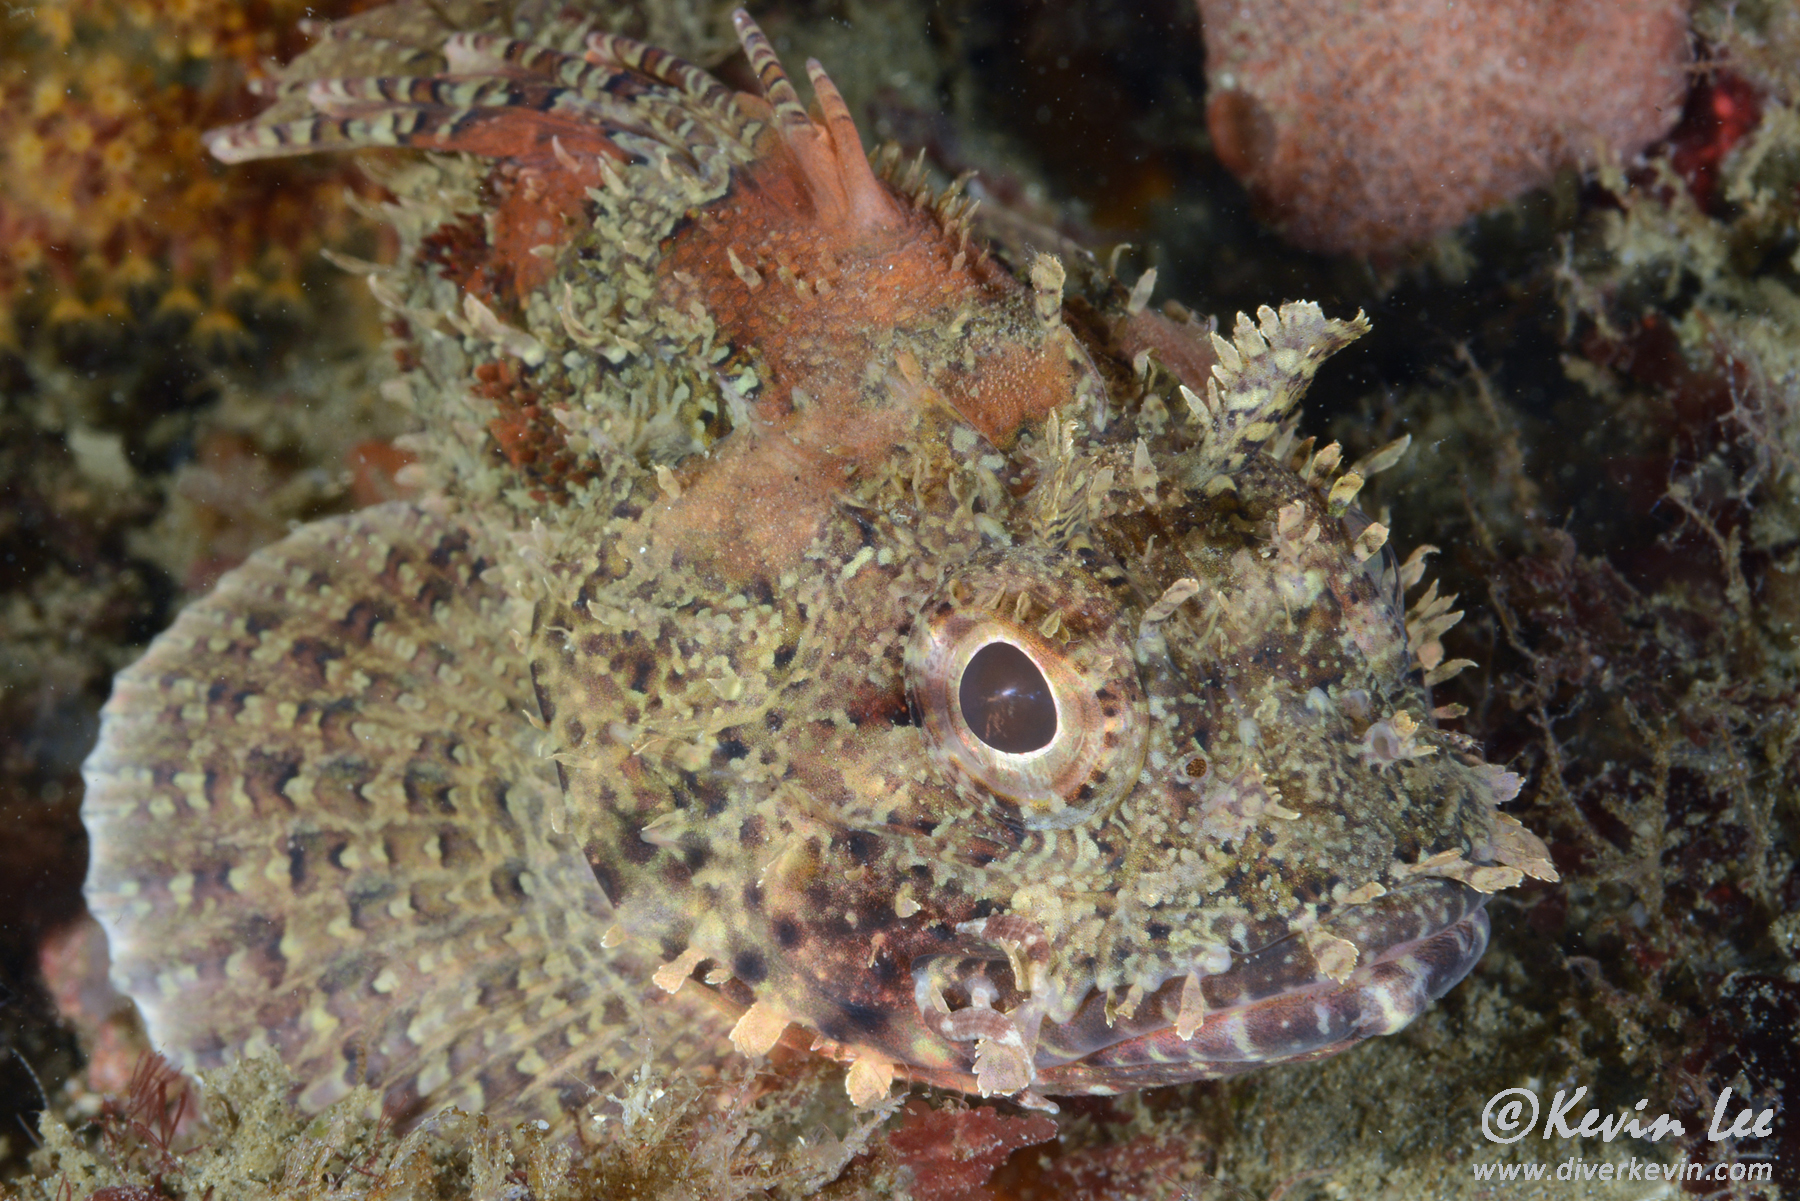
\includegraphics{cover_photo}~\\[1cm]
\pdftooltip{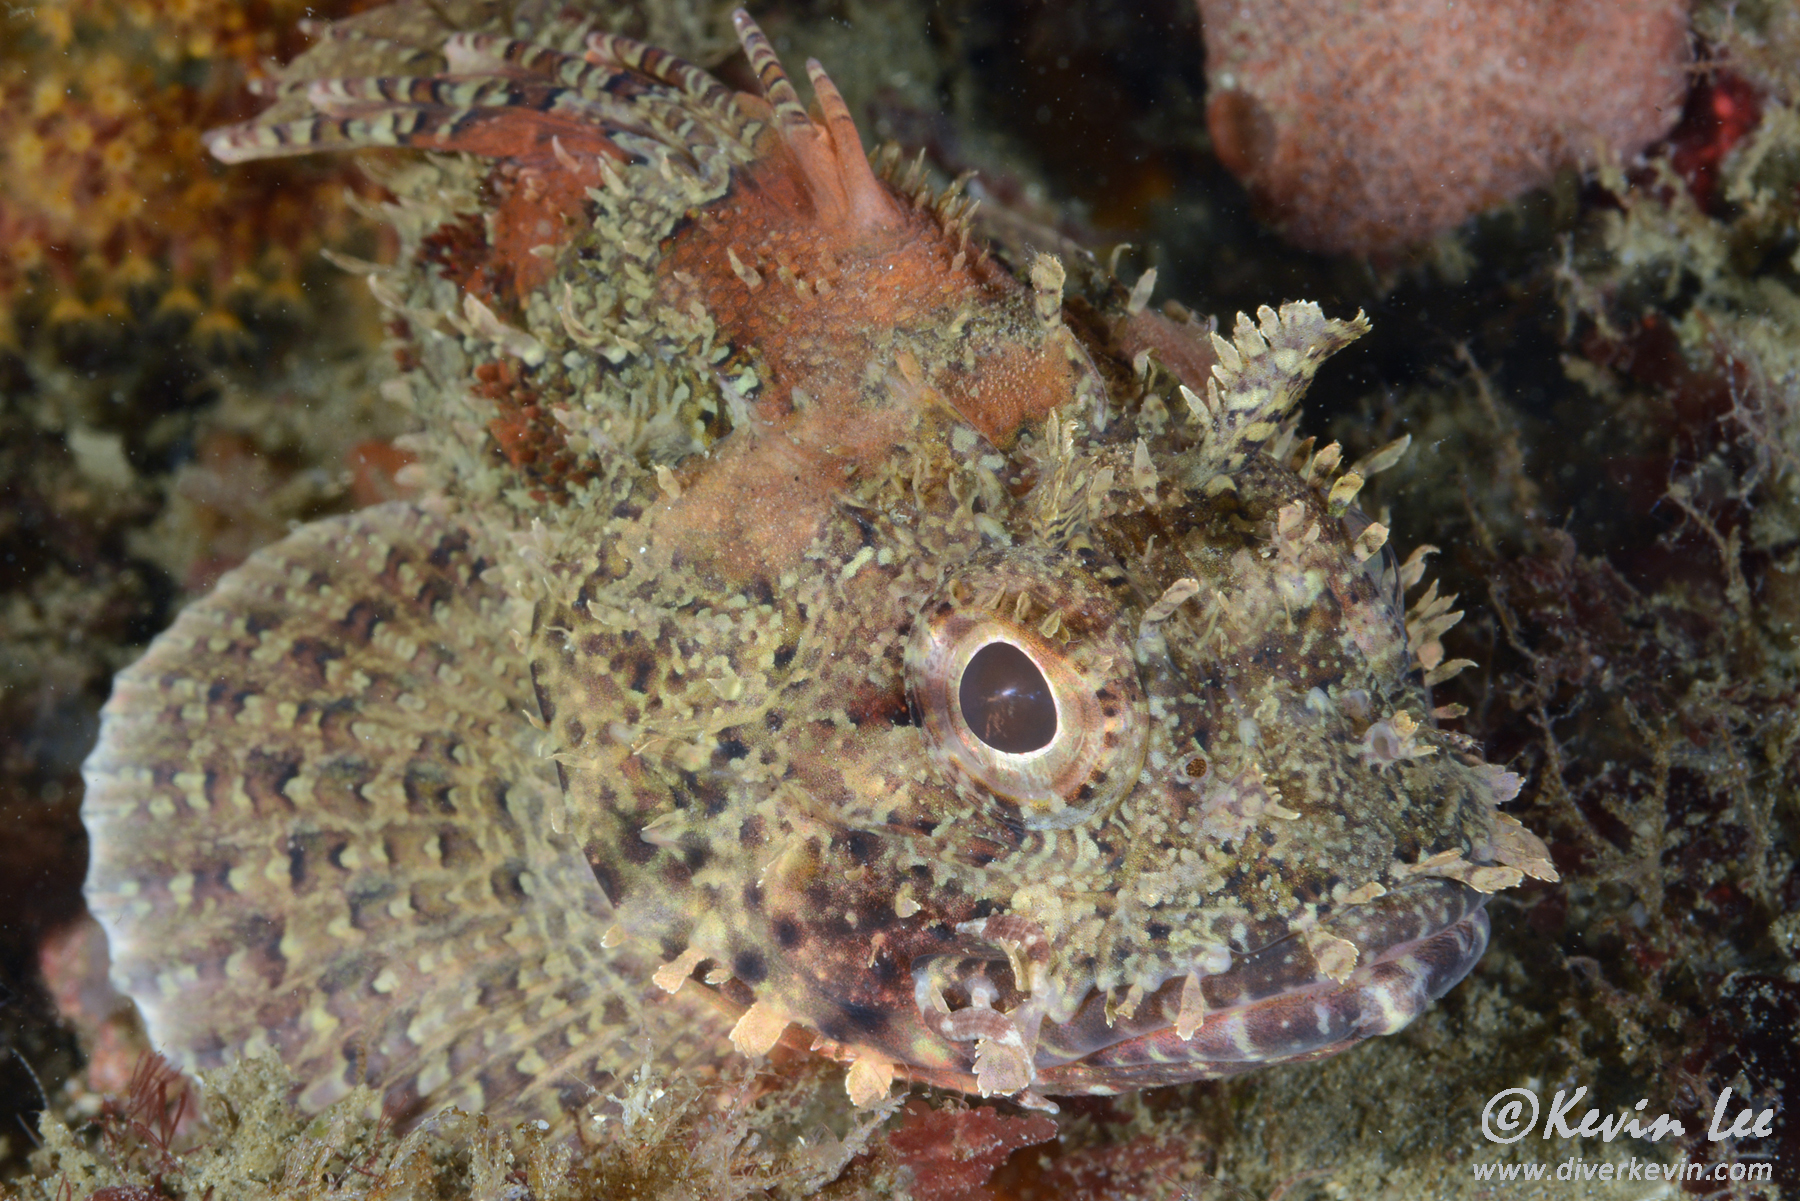
\includegraphics{cover_photo}}{This is a fish.}



Melissa H. Monk\textsuperscript{1}\\
Xi He\textsuperscript{1}\\
John Budrick\textsuperscript{2}\\

\vspace{.5cm}

\small
\textsuperscript{1}Southwest Fisheries Science Center, U.S. Department of Commerce, National Oceanic and Atmospheric Administration, National Marine Fisheries Service, 110 Shaffer Road, Santa Cruz, California 95060\\

\vspace{.3cm}

\textsuperscript{2}California Department of Fish and Wildlife, 350 Harbor Blvd., Belmont, California 94002\\


\vspace{.5cm}

\vfill
DRAFT SAFE\\
Disclaimer: This information is distributed solely for the purpose of pre-dissemination
peer review under applicable information quality guidelines. It has not been formally
disseminated by NOAA Fisheries. It does not represent and should not be construed to
represent any agency determination or policy. 

\vspace{.3cm}
%Bottom of the page
%{\large \today}

\maketitle

\pagenumbering{roman}
\setcounter{page}{1}
\end{center}

{
\setcounter{tocdepth}{4}
\tableofcontents
}
\setlength{\parskip}{5mm plus1mm minus1mm} \pagebreak

\pagenumbering{arabic} \setcounter{page}{1}
\renewcommand{\thefigure}{\alph{figure}}
\renewcommand{\thetable}{\alph{table}}

\section*{Executive Summary}\label{executive-summary}
\addcontentsline{toc}{section}{Executive Summary}

\subsection*{Stock}\label{stock}
\addcontentsline{toc}{subsection}{Stock}

This assessment reports the status of the California scorpionfish
(\emph{Scorpaena guttata}) resource in U.S. waters off the coast of the
California, Oregon, and Washington using data through 2016. Etc\ldots{}

\subsection*{Catches}\label{catches}
\addcontentsline{toc}{subsection}{Catches}

Catch figure(s) with fleets: (Figures
\ref{fig:Exec_catch1}-\ref{fig:Exec_catch3})\\
Catch table: (Table \ref{tab:Exec_catch})

\FloatBarrier

\begin{figure}[htbp]
\centering
\includegraphics{California_scorpionfish_2017_files/figure-latex/unnamed-chunk-13-1.pdf}
\caption{California scorpionfish landings history for the recreational
fleets. \label{fig:Exec_catch1}}
\end{figure}

\begin{figure}[htbp]
\centering
\includegraphics{California_scorpionfish_2017_files/figure-latex/unnamed-chunk-14-1.pdf}
\caption{Stacked line plot of California scorpionfish landings history
for the commercial fleets. \label{fig:Exec_catch2}}
\end{figure}

\begin{figure}[htbp]
\centering
\includegraphics{California_scorpionfish_2017_files/figure-latex/unnamed-chunk-15-1.pdf}
\caption{Stacked line plot of California scorpionfish landings history
by region, north of Pt. Conception, between Pt. Conception and the
U.S.-Mexico border, and Mexican waters. \label{fig:Exec_catch3}}
\end{figure}

\FloatBarrier

\begin{figure}[htbp]
\centering
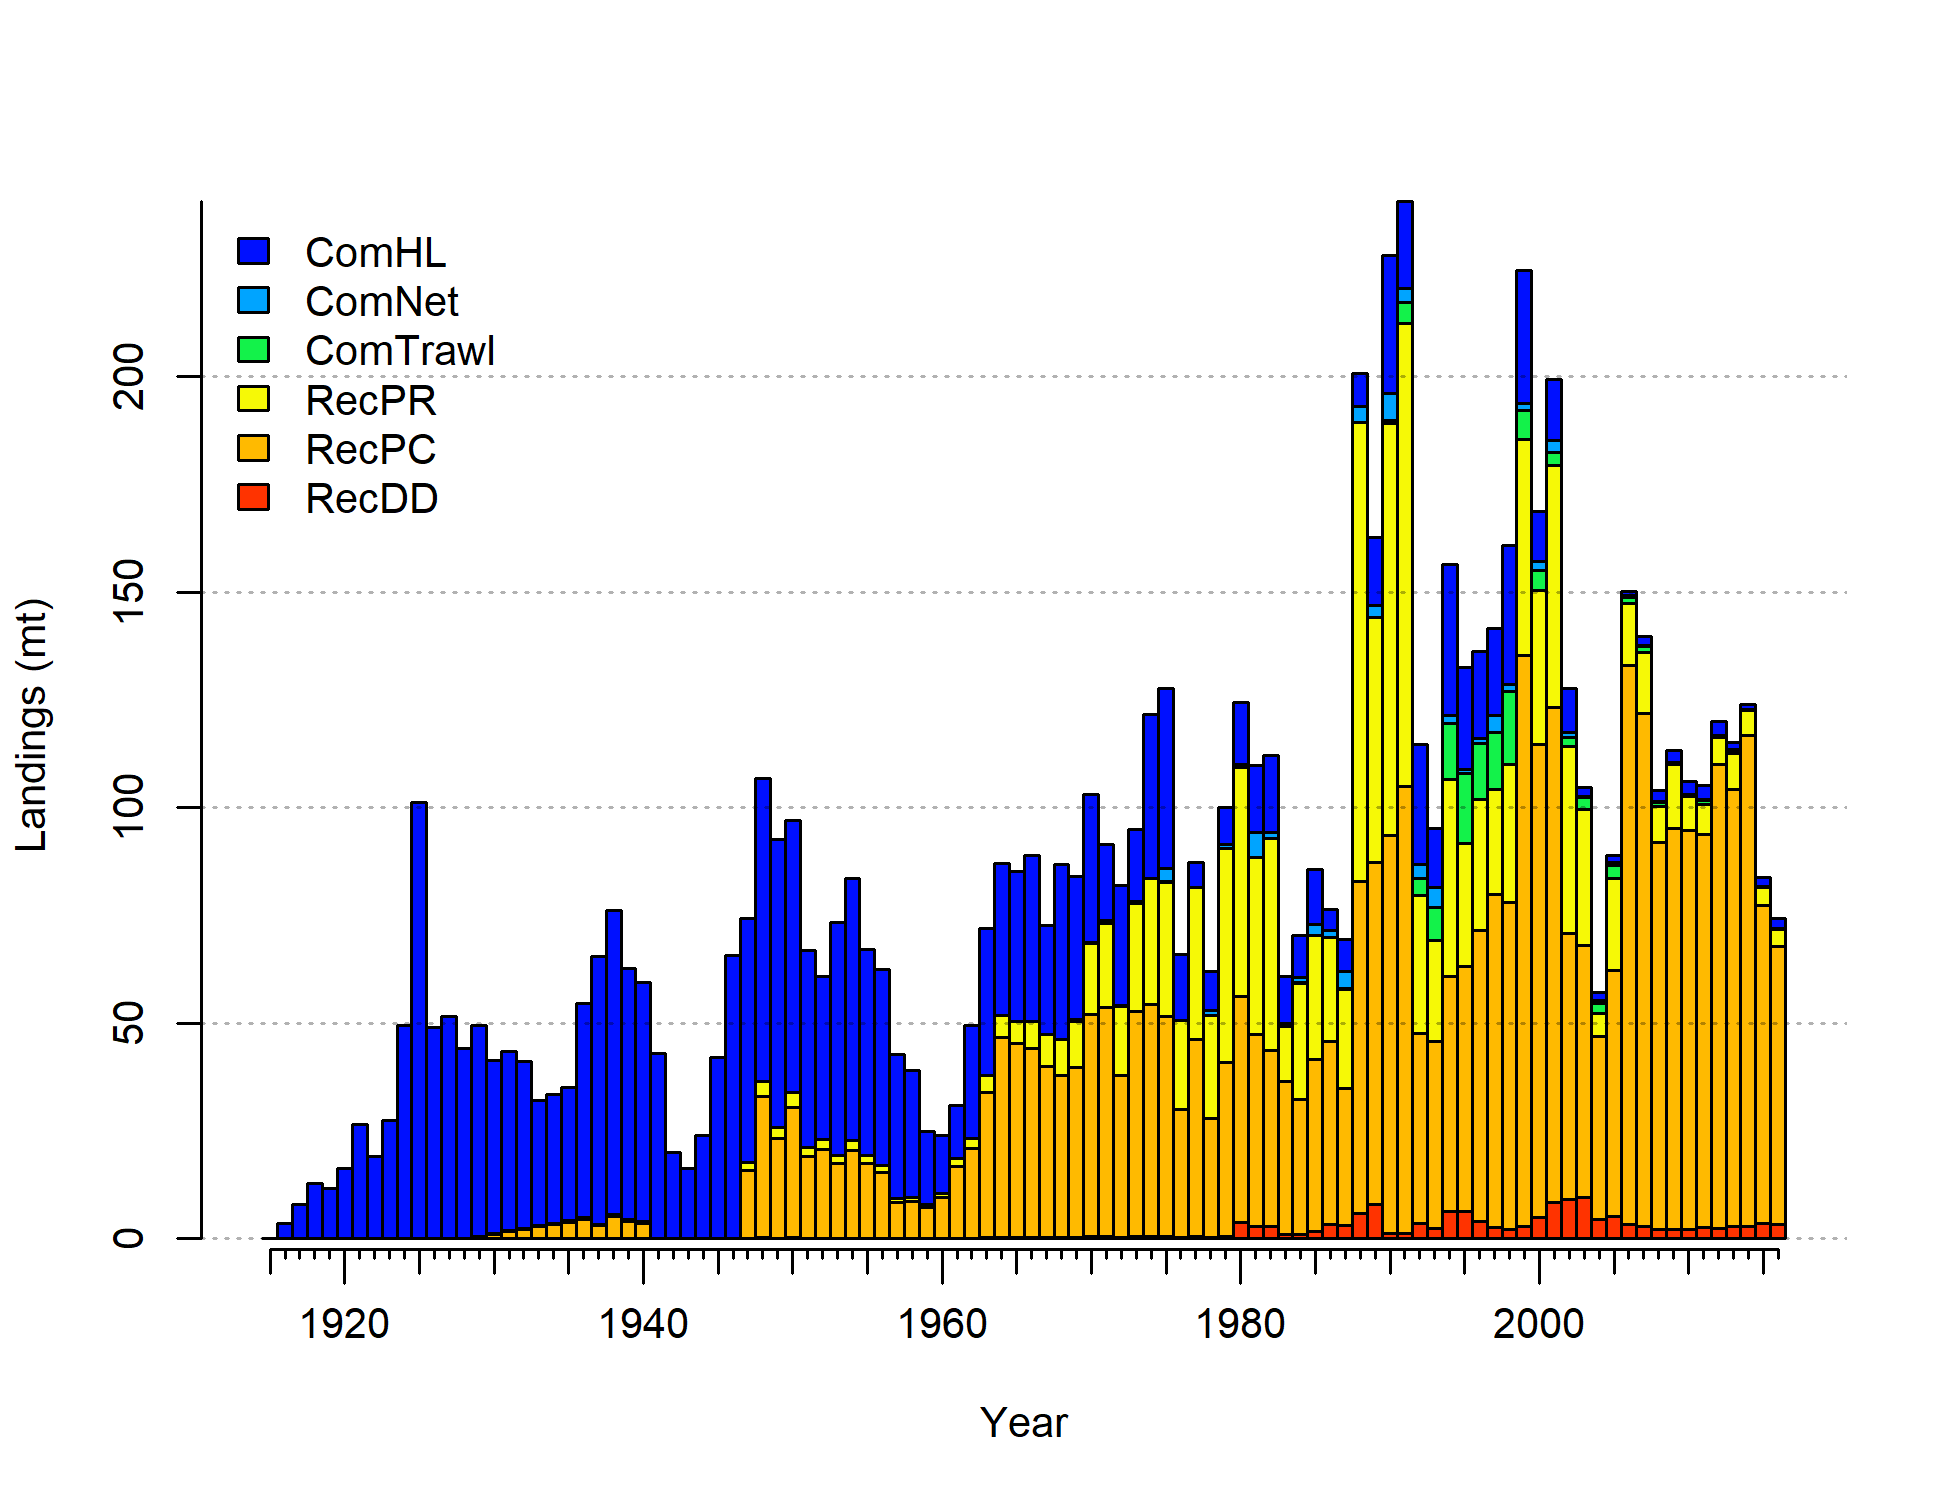
\includegraphics{r4ss/plots_mod1/catch2 landings stacked.png}
\caption{Landings history of California scorpionfish in the base model.
\label{fig:r4ss_catches}}
\end{figure}

\begin{table}[ht]
\centering
\caption{Recent California scorpionfish landings (mt) by 
                                            recreational (Rec.) and commercial (Com.) fleets.} 
\label{tab:Exec_catch}
\begin{tabular}{l>{\centering}p{.6in}>{\centering}p{1.1in}>{\centering}p{.9in}>{\centering}p{1.1in}>{\centering}p{.5in}>{\centering}p{.5in}>{\centering}p{.5in}}
  \hline
Year & Rec. Private & Rec. Party/Charter & Rec. Dead Discards & Com. Hook-and-line & Com. Trawl & Com. Gillnet & Total \\ 
  \hline
2007 & 14.24 & 118.87 & 2.89 & 1.90 & 1.48 & 0.21 & 139.58 \\ 
  2008 & 8.38 & 89.65 & 2.25 & 2.46 & 0.86 & 0.28 & 103.89 \\ 
  2009 & 14.68 & 93.16 & 2.09 & 2.97 & 0.27 & 0.13 & 113.31 \\ 
  2010 & 8.07 & 92.55 & 2.03 & 2.99 & 0.18 & 0.14 & 105.97 \\ 
  2011 & 6.84 & 91.18 & 2.66 & 3.24 & 1.05 & 0.24 & 105.21 \\ 
  2012 & 6.22 & 107.63 & 2.34 & 3.22 & 0.43 & 0.18 & 120.00 \\ 
  2013 & 8.18 & 101.31 & 2.94 & 1.73 & 0.83 & 0.14 & 115.14 \\ 
  2014 & 5.88 & 113.83 & 2.93 & 1.03 & 0.13 & 0.04 & 123.82 \\ 
  2015 & 4.15 & 73.78 & 3.59 & 2.21 & 0.13 & 0.03 & 83.89 \\ 
  2016 & 3.86 & 64.56 & 3.29 & 2.32 & 0.13 & 0.00 & 74.16 \\ 
   \hline
\end{tabular}
\end{table}

\FloatBarrier

\newpage

\subsection*{Data and Assessment}\label{data-and-assessment}
\addcontentsline{toc}{subsection}{Data and Assessment}

California scorpionfish was assessed in 2005 (Maunder et al.
\protect\hyperlink{ref-Maunder2005}{2005}) using Stock Synthesis II
version 1.18. This assessment uses the newest version of Stock Synthesis
(3.30.0.4). The model begins in 1916, and assumes the stock was at an
unfished equilibrium that year.

Map of assessment region: (Figure \ref{fig:assess_region_map}).

\begin{figure}[htbp]
\centering
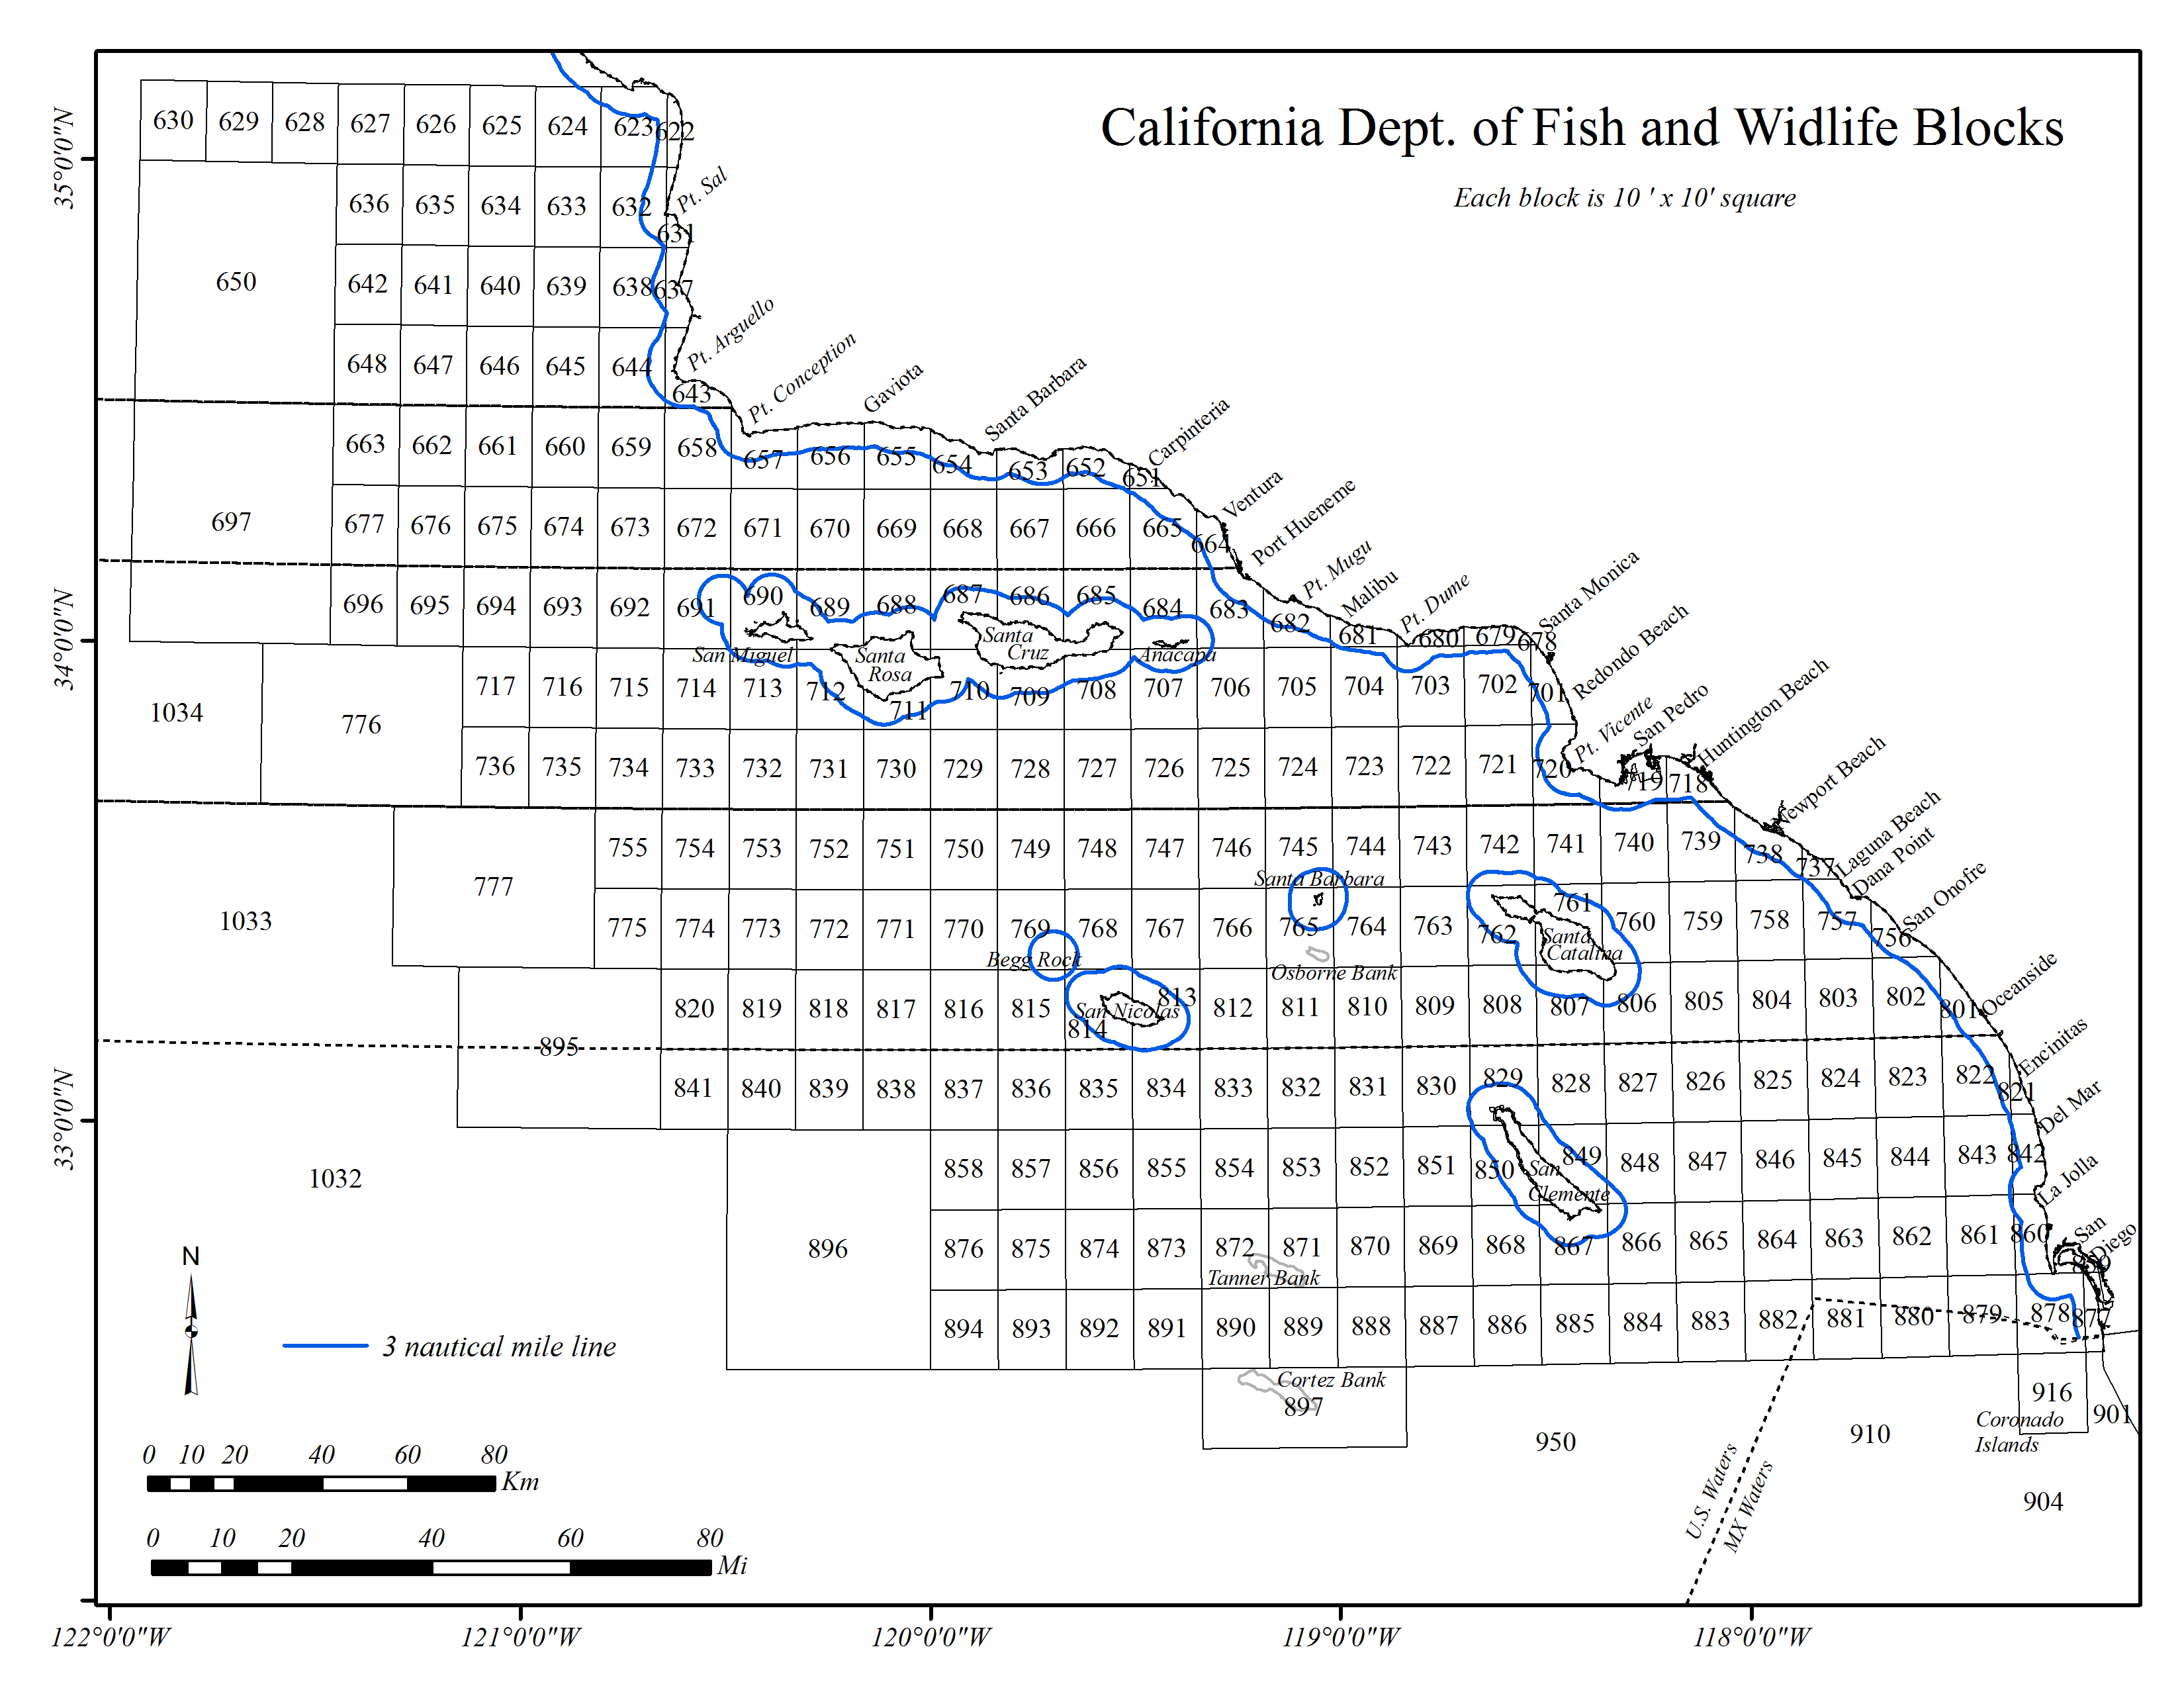
\includegraphics{Figures/assess_region_map.png}
\caption{Map depicting the boundaries for the base-case model.
\label{fig:assess_region_map}}
\end{figure}

\FloatBarrier

\subsection*{Stock Biomass}\label{stock-biomass}
\addcontentsline{toc}{subsection}{Stock Biomass}

Spawning output Figure: Figure \ref{fig:Spawnbio_all}\\
Spawning output Table(s): Table \ref{tab:SpawningDeplete_mod1}\\
Relative depletion Figure: Figure \ref{fig:RelDeplete_all}

The estimated relative depletion level (spawning output relative to
unfished spawning output) of the the base-case model in 2016 is 55.6\%
(\textasciitilde{}95\% asymptotic interval: \(\pm\) 40.5\%-70.7\%)
(Figure \ref{fig:RelDeplete_all}).

\FloatBarrier

\begin{table}[ht]
\centering
\caption{Recent trend in beginning of the 
                                      year spawning output and depletion for
                                      the base model for California scorpionfish.} 
\label{tab:SpawningDeplete_mod1}
\begin{tabular}{l>{\centering}p{1.3in}>{\centering}p{1.2in}>{\centering}p{1in}>{\centering}p{1.2in}}
  \hline
Year & Spawning Output (mt) & \~{} 95\% confidence interval & Estimated depletion & \~{} 95\% confidence interval \\ 
  \hline
2008 & 649.288 & (339.09-959.49) & 0.731 & (0.554-0.908) \\ 
  2009 & 632.086 & (332.7-931.47) & 0.712 & (0.542-0.881) \\ 
  2010 & 599.904 & (317.76-882.05) & 0.676 & (0.518-0.833) \\ 
  2011 & 570.013 & (305.72-834.31) & 0.642 & (0.498-0.786) \\ 
  2012 & 546.582 & (296.38-796.78) & 0.616 & (0.484-0.747) \\ 
  2013 & 511.635 & (276.25-747.02) & 0.576 & (0.454-0.698) \\ 
  2014 & 467.039 & (249.44-684.64) & 0.526 & (0.413-0.639) \\ 
  2015 & 425.087 & (219.81-630.37) & 0.479 & (0.367-0.59) \\ 
  2016 & 431.582 & (218.81-644.35) & 0.486 & (0.366-0.606) \\ 
  2017 & 493.509 & (242.88-744.14) & 0.556 & (0.405-0.707) \\ 
   \hline
\end{tabular}
\end{table}

\FloatBarrier

\begin{figure}[htbp]
\centering
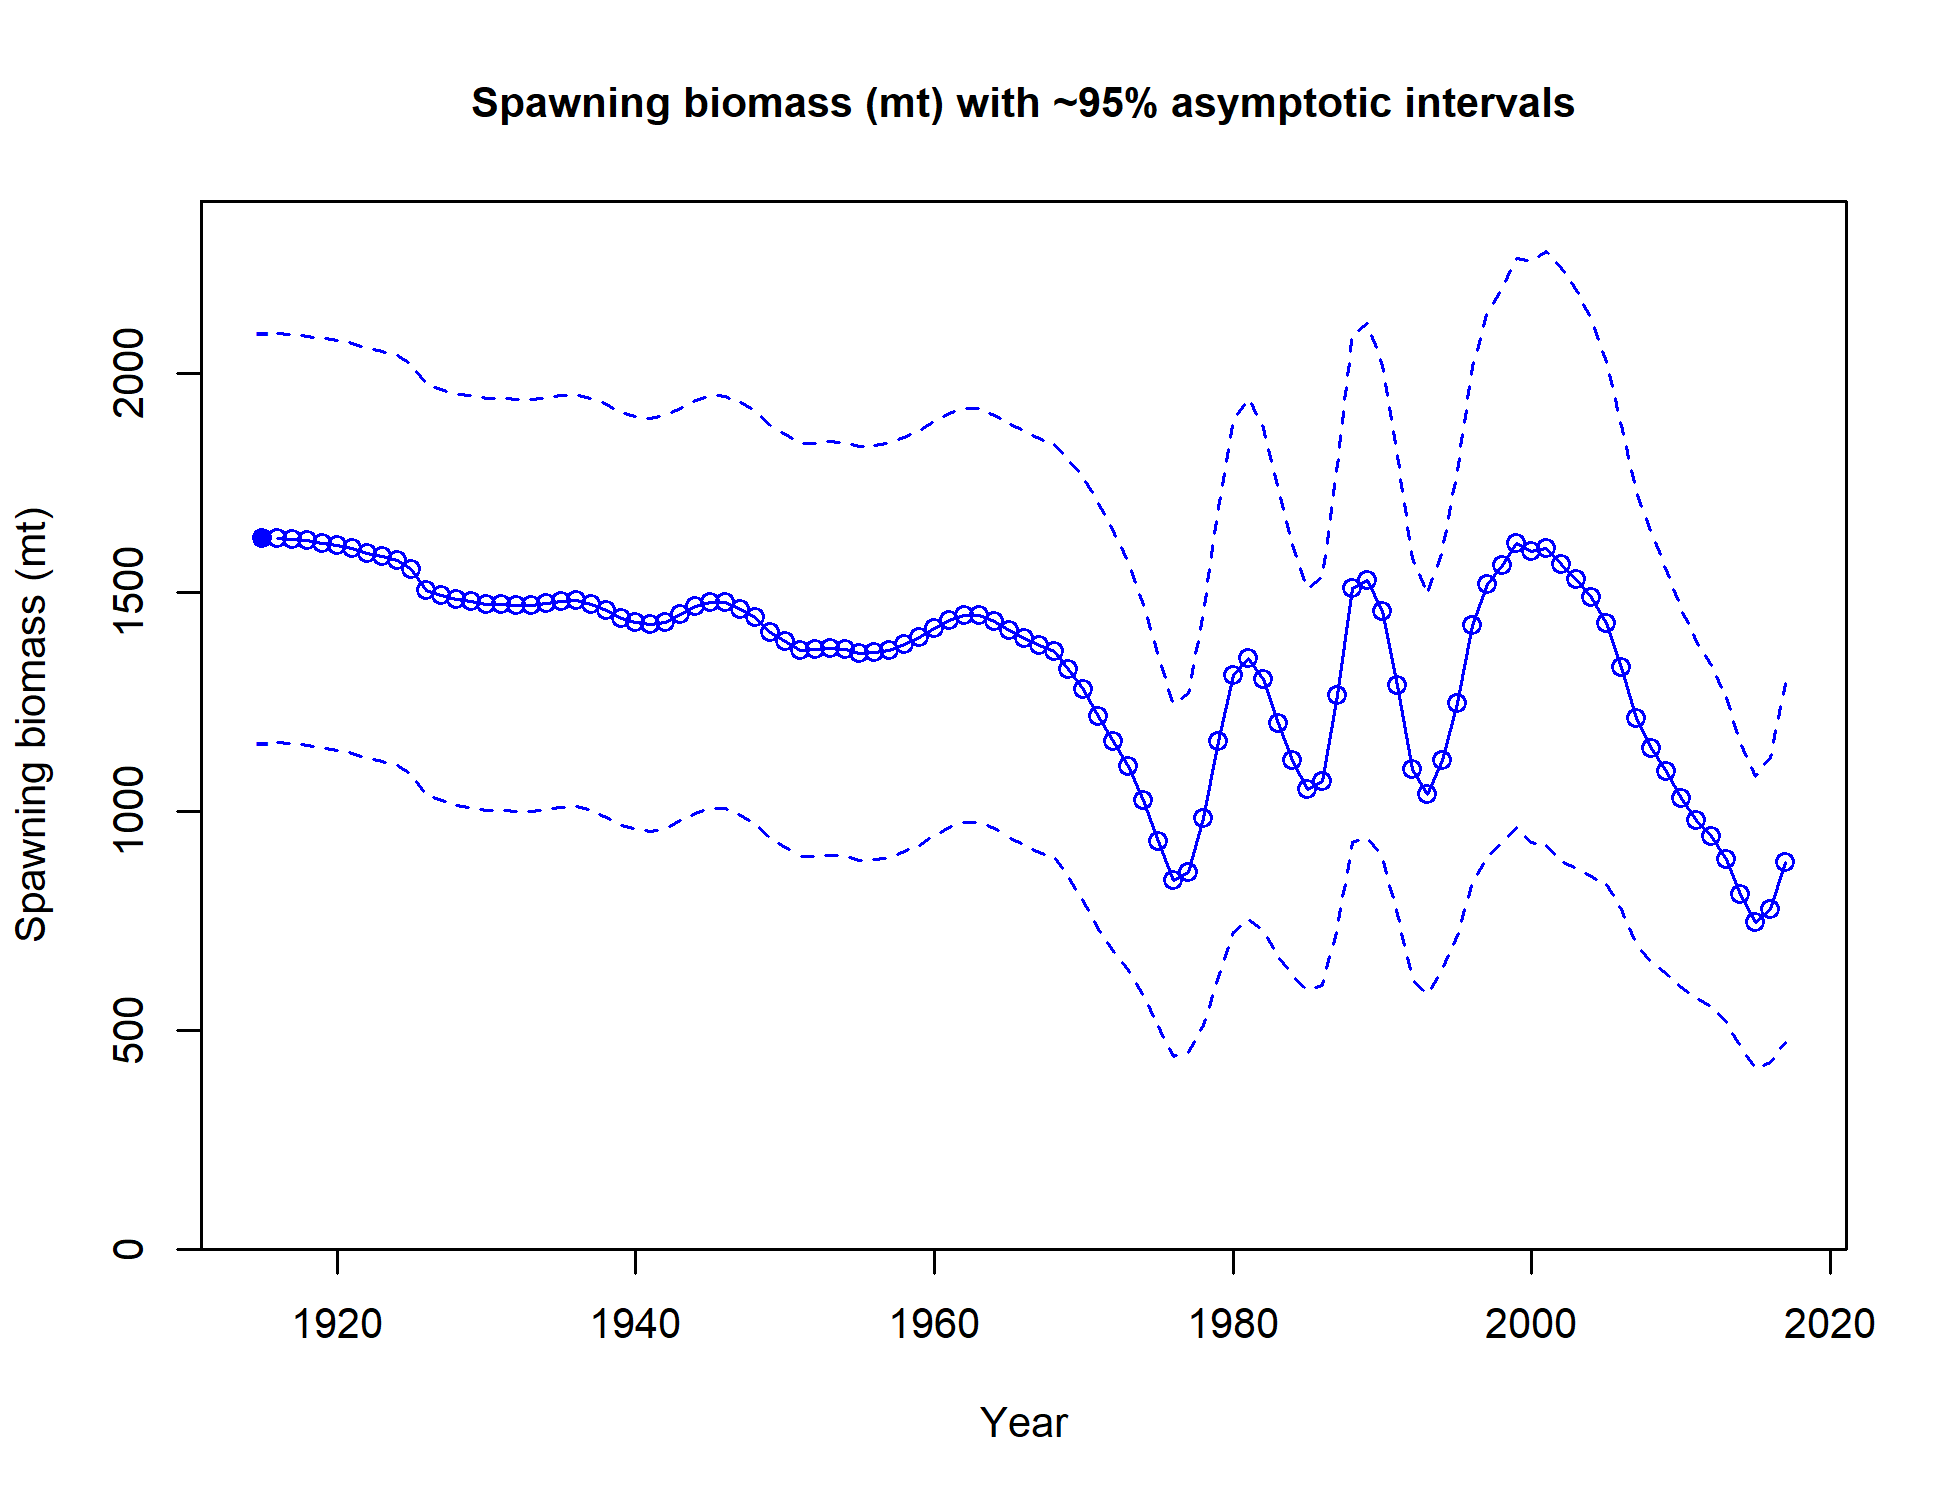
\includegraphics{r4ss/plots_mod1/ts7_Spawning_biomass_(mt)_with_95_asymptotic_intervals_intervals.png}
\caption{Time series of spawning output trajectory (circles and line:
median; light broken lines: 95\% credibility intervals) for the base
case assessment model. \label{fig:Spawnbio_all}}
\end{figure}

\begin{figure}[htbp]
\centering
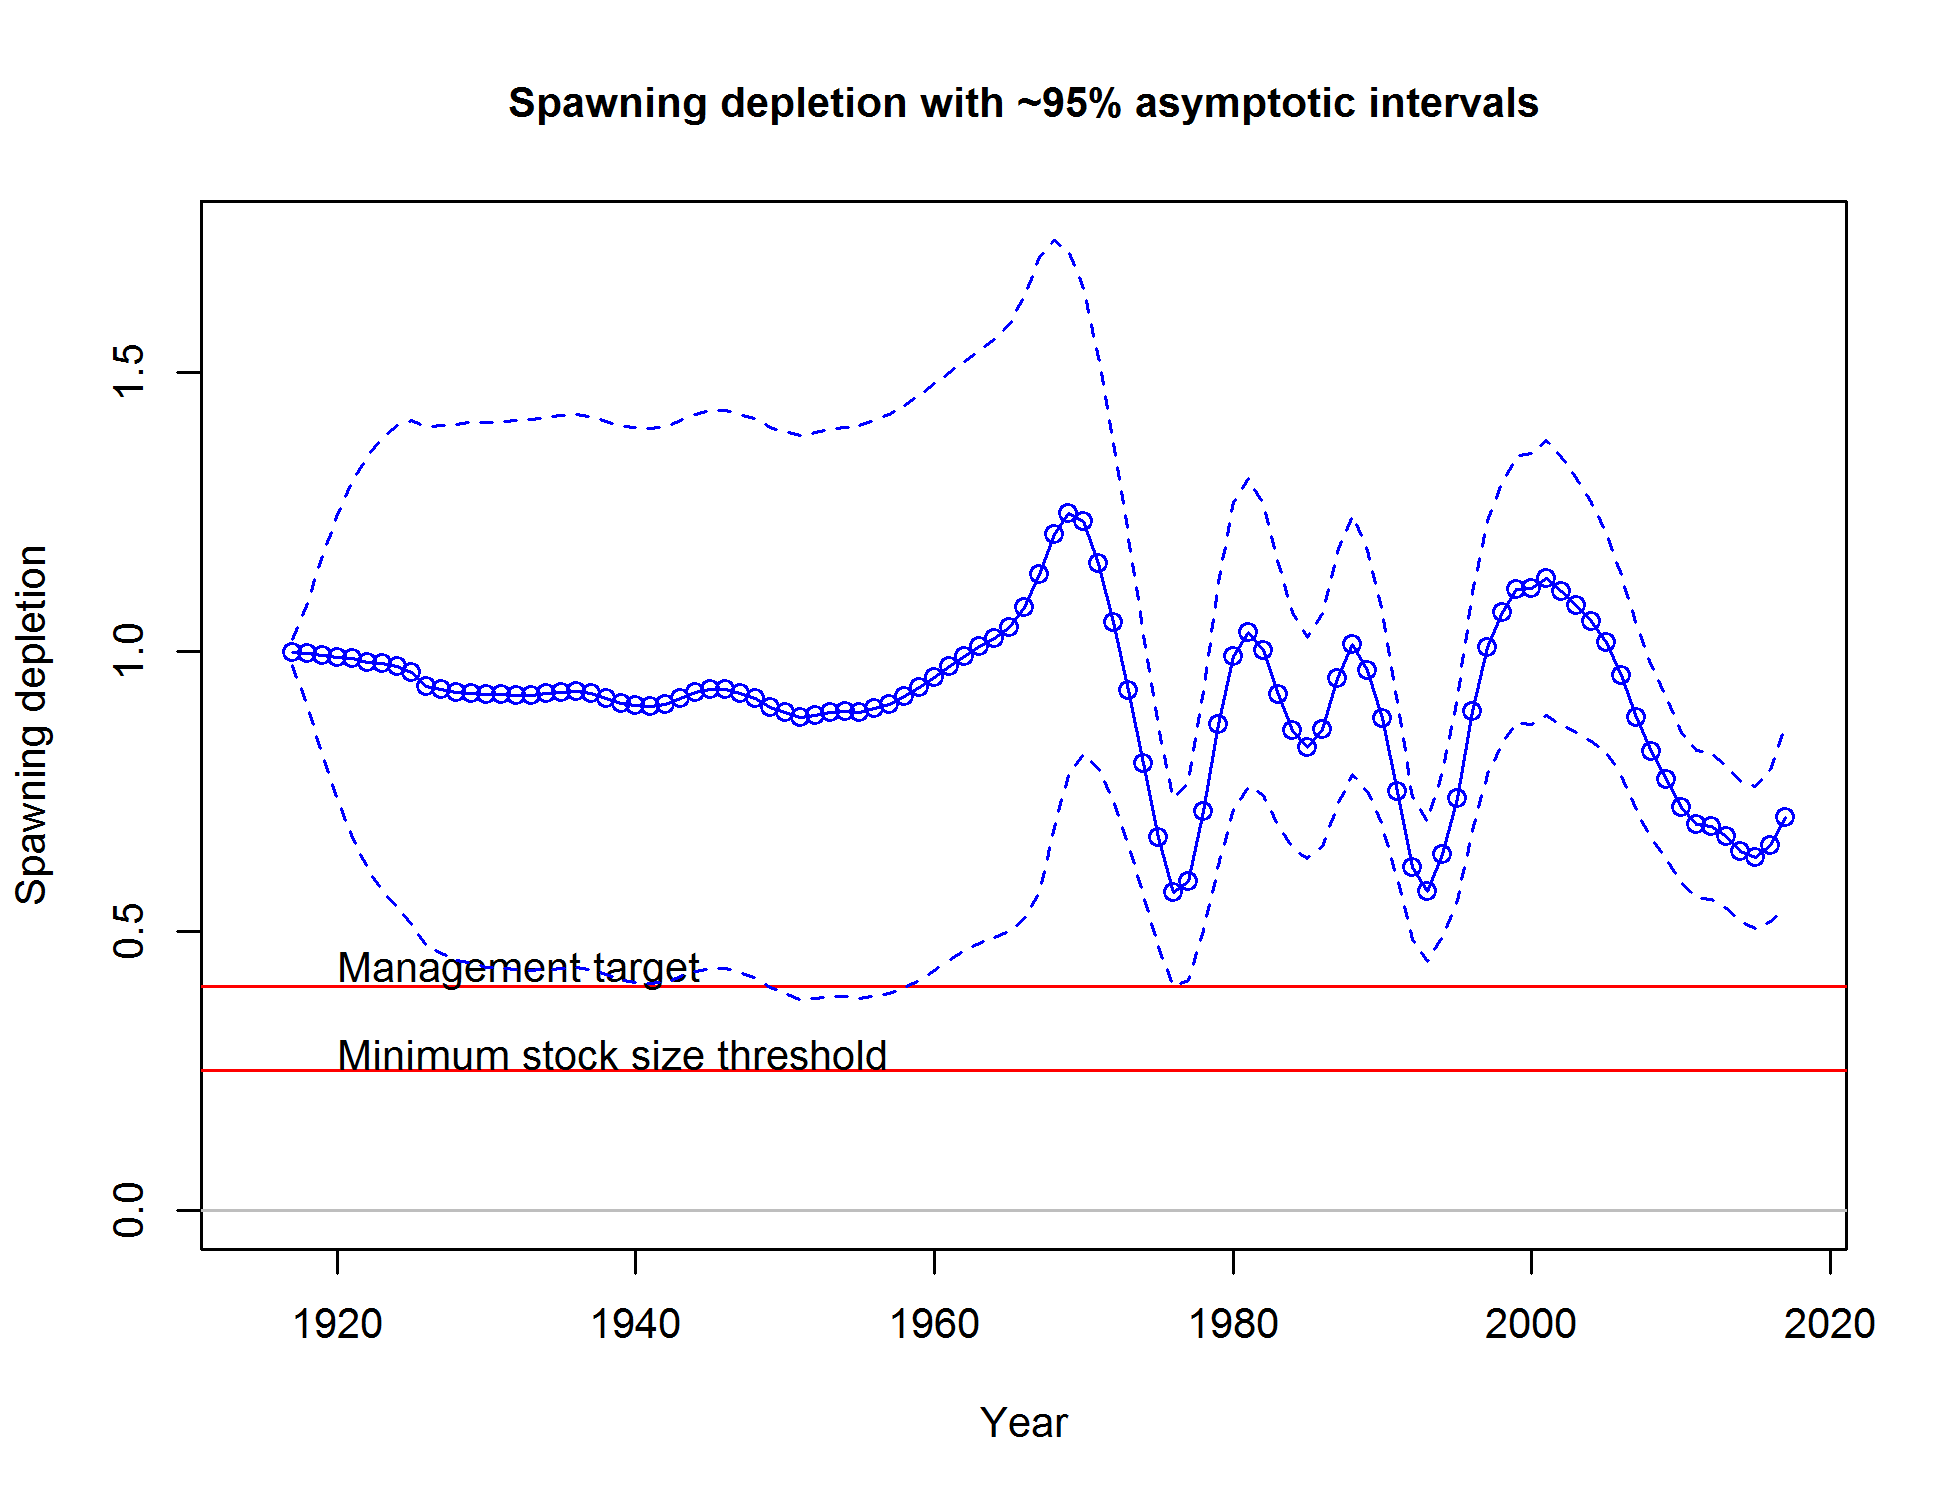
\includegraphics{r4ss/plots_mod1/ts9_Spawning_depletion_with_95_asymptotic_intervals_intervals.png}
\caption{Estimated relative depletion with approximate 95\% asymptotic
confidnce intervals (dashed lines) for the base case assessment model.
\label{fig:RelDeplete_all}}
\end{figure}

\FloatBarrier

\subsection*{Recruitment}\label{recruitment}
\addcontentsline{toc}{subsection}{Recruitment}

Recruitment Figure: (Figure \ref{fig:Recruits_all})\\
Recruitment Tables: (Tables \ref{tab:Recruit_mod1}

\begin{table}[ht]
\centering
\caption{Recent recruitment for the base model.} 
\label{tab:Recruit_mod1}
\begin{tabular}{>{\centering}p{.8in}>{\centering}p{1.6in}>{\centering}p{1.3in}}
  \hline
Year & Estimated Recruitment (1,000s) & \~{} 95\% confidence interval \\ 
  \hline
2008 & 2075.83 & (890.89 - 4836.82) \\ 
  2009 & 3042.65 & (1409.75 - 6566.92) \\ 
  2010 & 2050.82 & (836.7 - 5026.71) \\ 
  2011 & 1178.75 & (455.92 - 3047.56) \\ 
  2012 & 1296.70 & (508.76 - 3304.96) \\ 
  2013 & 3459.48 & (1487.4 - 8046.27) \\ 
  2014 & 3795.50 & (1434.21 - 10044.44) \\ 
  2015 & 7788.63 & (2862.54 - 21191.93) \\ 
  2016 & 2994.58 & (886.82 - 10111.95) \\ 
  2017 & 3064.95 & (907.96 - 10346.18) \\ 
   \hline
\end{tabular}
\end{table}

\FloatBarrier

\begin{figure}[htbp]
\centering
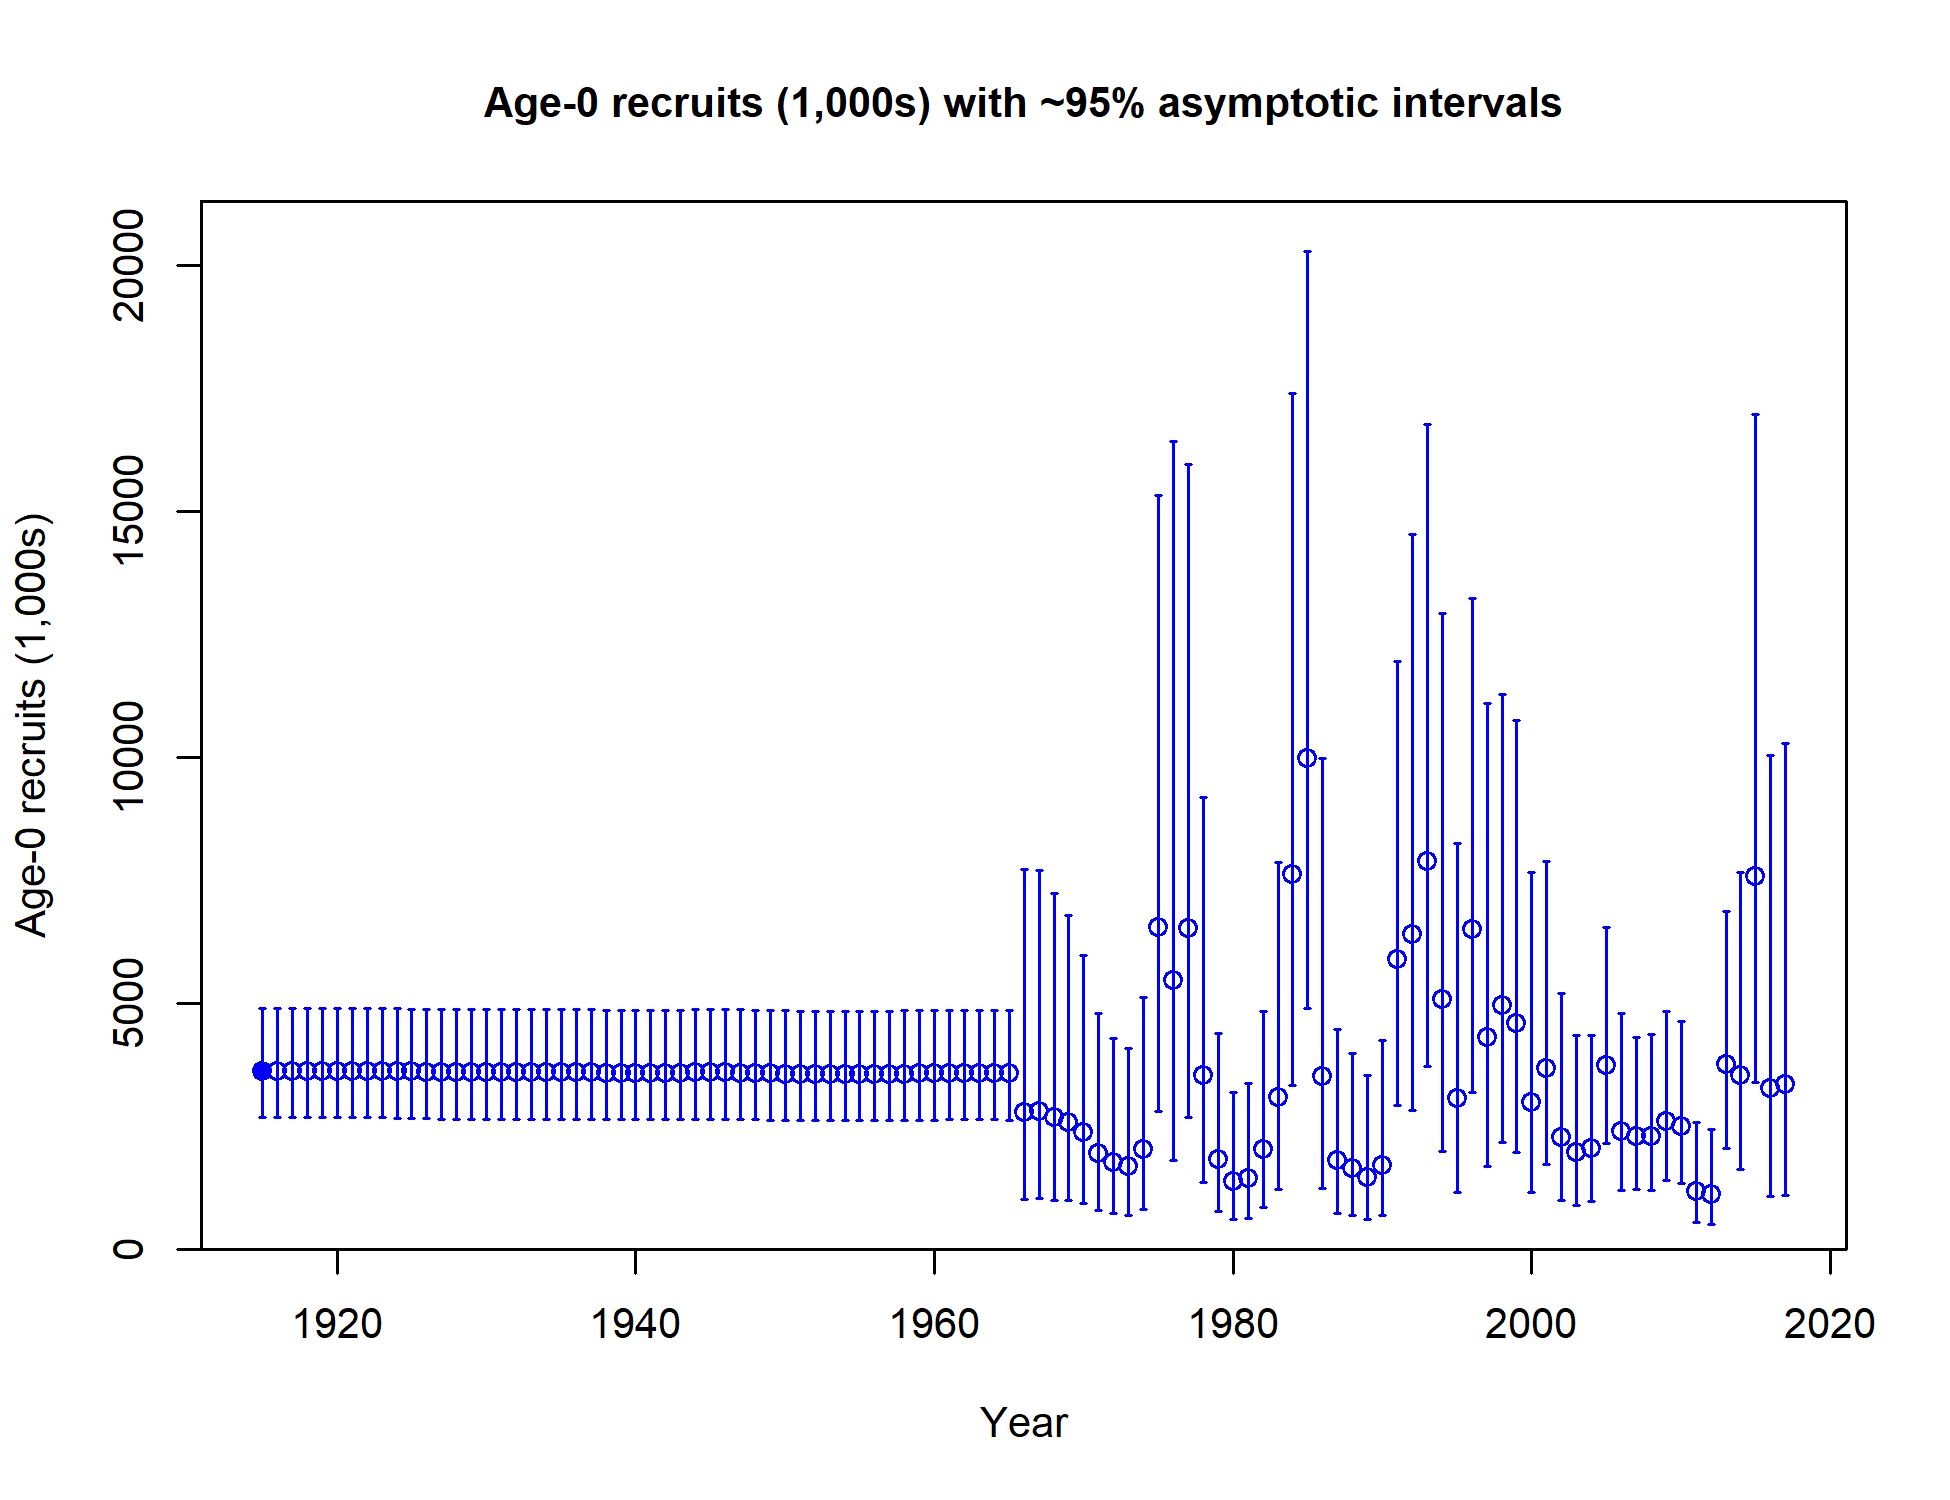
\includegraphics{r4ss/plots_mod1/ts11_Age-0_recruits_(1000s)_with_95_asymptotic_intervals.png}
\caption{Time series of estimated California scorpionfish recruitments
for the base-case model with 95\% confidence or credibility intervals.
\label{fig:Recruits_all}}
\end{figure}

\FloatBarrier

\subsection*{Exploitation status}\label{exploitation-status}
\addcontentsline{toc}{subsection}{Exploitation status}

Exploitation Tables: Table \ref{tab:SPR_Exploit_mod1} Exploitation
Figure: Figure \ref{fig:SPR_all}).

A summary of California scorpionfish exploitation histories for base
model is provided as Figure .

\FloatBarrier

\begin{table}[ht]
\centering
\caption{Recent trend in spawning potential 
                                        ratio and exploitation for California scorpionfish in the base model.  Fishing intensity is (1-SPR) 
                                        divided by 50\% (the SPR target) and exploitation 
                                        is F divided by F\textsubscript{SPR}.} 
\label{tab:SPR_Exploit_mod1}
\begin{tabular}{l>{\centering}p{1in}>{\centering}p{1.2in}>{\centering}p{1in}>{\centering}p{1.2in}}
  \hline
Year & Fishing intensity & \~{} 95\% confidence interval & Exploitation rate & \~{} 95\% confidence interval \\ 
  \hline
2007 & 0.53 & (0.29-0.78) & 0.08 & (0.04-0.11) \\ 
  2008 & 0.46 & (0.23-0.69) & 0.06 & (0.03-0.09) \\ 
  2009 & 0.50 & (0.26-0.75) & 0.07 & (0.04-0.1) \\ 
  2010 & 0.49 & (0.26-0.73) & 0.07 & (0.04-0.1) \\ 
  2011 & 0.51 & (0.27-0.75) & 0.07 & (0.04-0.1) \\ 
  2012 & 0.57 & (0.32-0.83) & 0.08 & (0.05-0.12) \\ 
  2013 & 0.58 & (0.32-0.84) & 0.09 & (0.05-0.13) \\ 
  2014 & 0.64 & (0.37-0.91) & 0.10 & (0.05-0.14) \\ 
  2015 & 0.53 & (0.28-0.78) & 0.07 & (0.03-0.1) \\ 
  2016 & 0.50 & (0.26-0.74) & 0.05 & (0.02-0.08) \\ 
   \hline
\end{tabular}
\end{table}

\FloatBarrier

\begin{figure}[htbp]
\centering
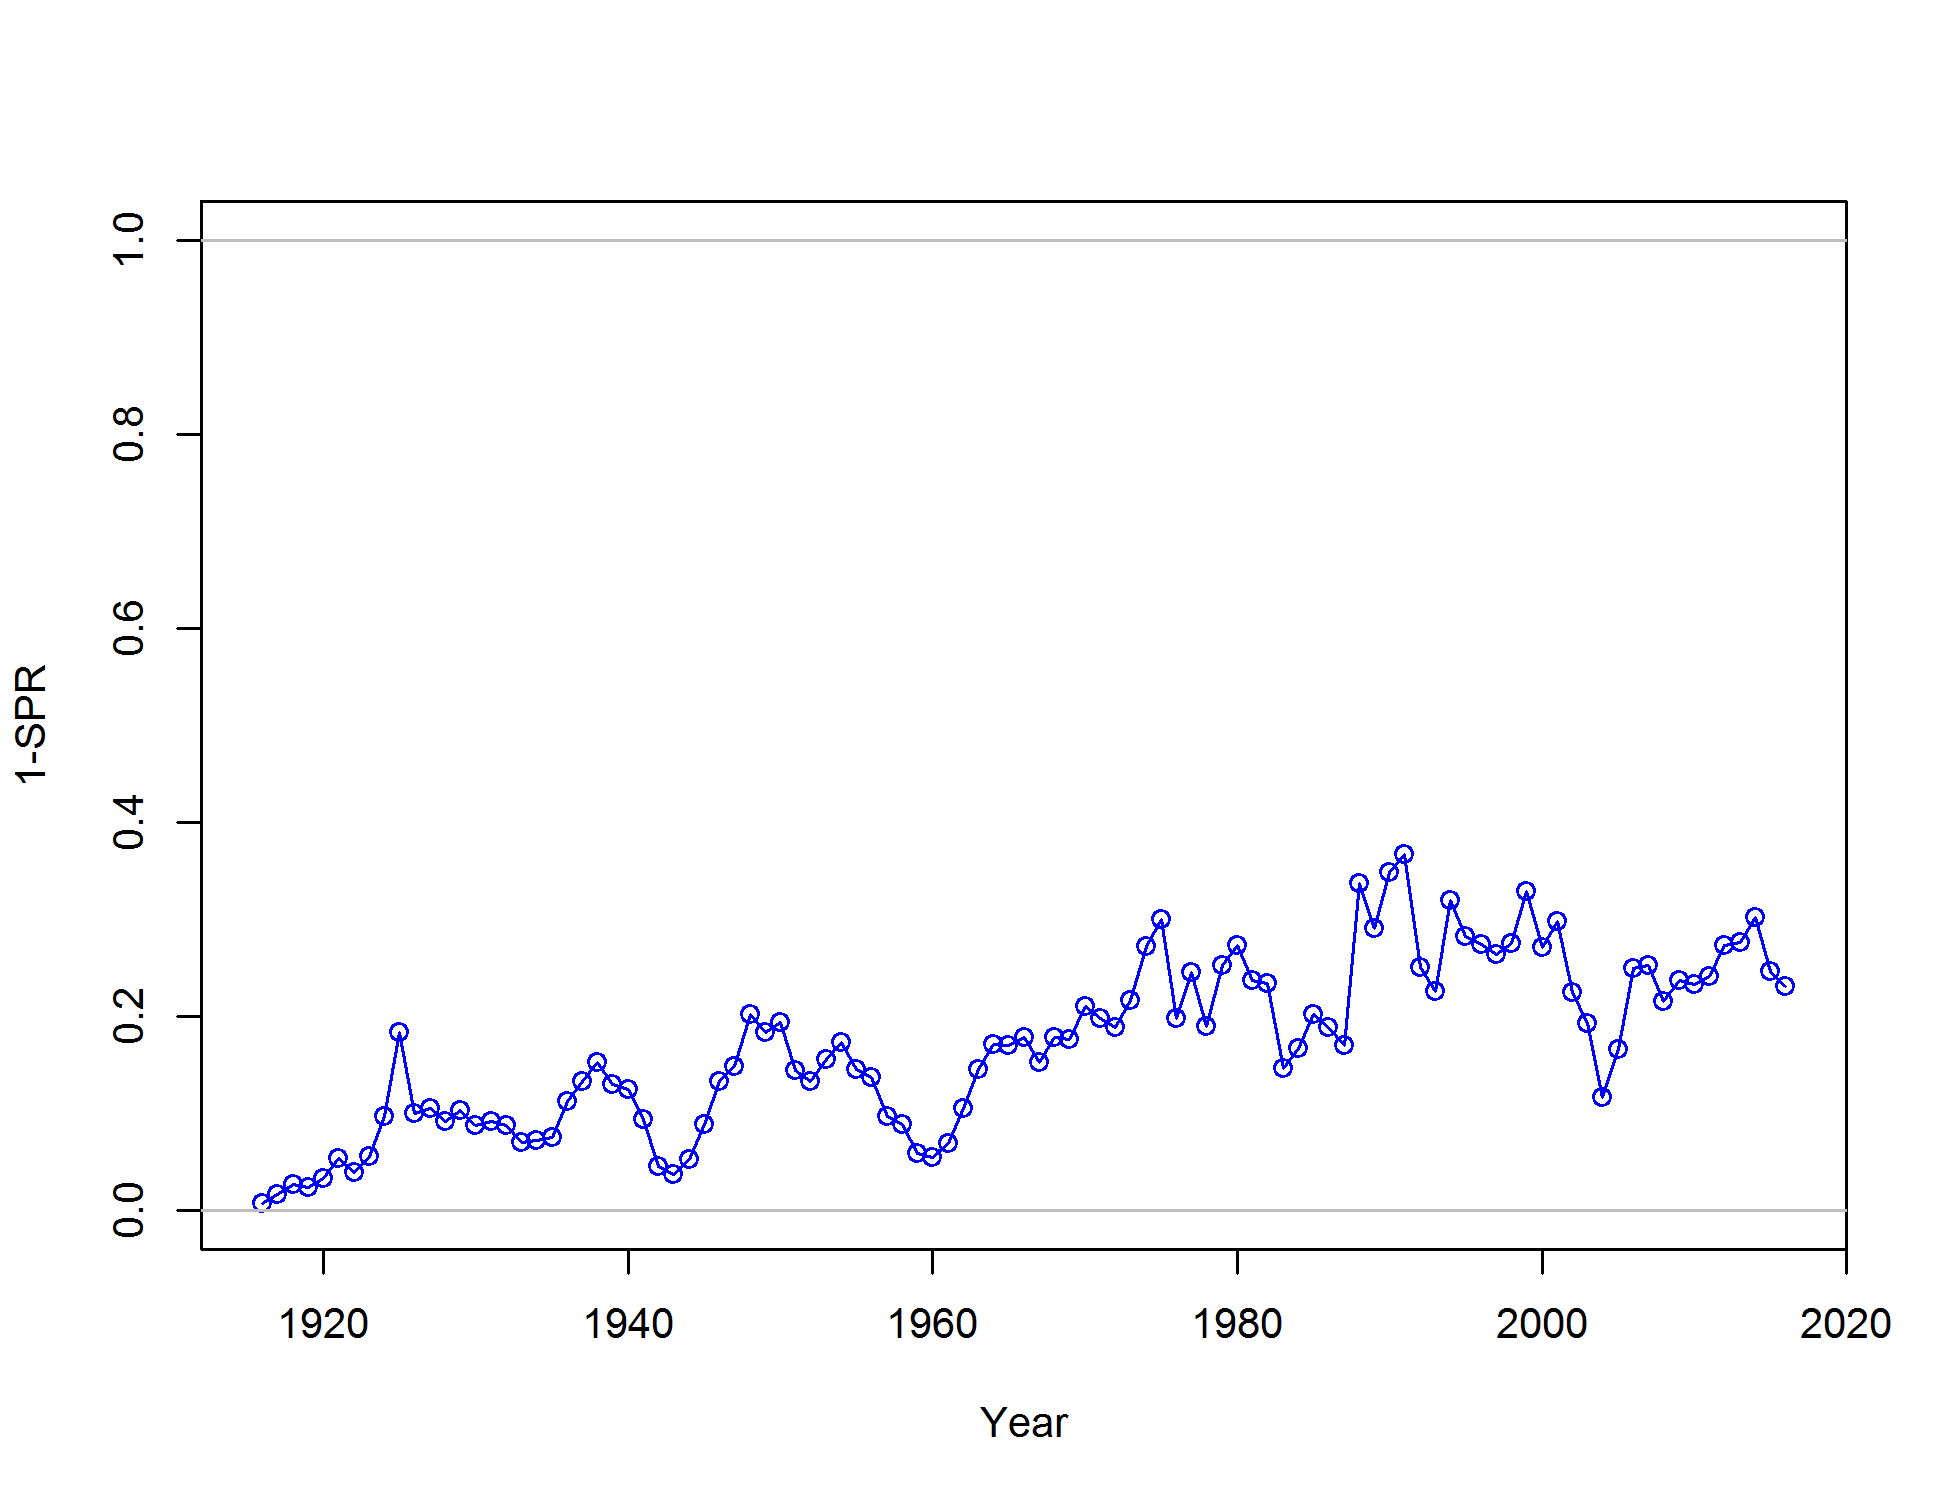
\includegraphics{r4ss/plots_mod1/SPR2_minusSPRseries.png}
\caption{Estimated spawning potential ratio (SPR) for the base-case
model. One minus SPR is plotted so that higher exploitation rates occur
on the upper portion of the y-axis. The management target is plotted as
a red horizontal line and values above this reflect harvests in excess
of the overfishing proxy based on the SPR\textsubscript{50\%} harvest
rate. The last year in the time series is 2016. \label{fig:SPR_all}}
\end{figure}

\FloatBarrier

\subsection*{Ecosystem Considerations}\label{ecosystem-considerations}
\addcontentsline{toc}{subsection}{Ecosystem Considerations}

In this assessment, ecosystem considerations were\ldots{}..

\subsection*{Reference Points}\label{reference-points}
\addcontentsline{toc}{subsection}{Reference Points}

This stock assessment estimates that California scorpionfish in the base
model are above the biomass target, but above the minimum stock size
threshold. \hl{Add sentence about spawning output trend.} The estimated
relative depletion level for \hl{Model 1} in 2016 is 55.6\%
(\textasciitilde{}95\% asymptotic interval: \(\pm\) 40.5\%-70.7\%,
corresponding to an unfished spawning output of 493.509 mt
(\textasciitilde{}95\% asymptotic interval: 242.88-744.14 mt) of
spawning output in the base model (Table \ref{tab:Ref_pts_mod1}).
Unfished age 1+ biomass was estimated to be 2218.6 mt in the base case
model. The target spawning output based on the biomass target
(\(SB_{40\%}\)) is 355.2 mt, which gives a catch of 218.4 mt.
Equilibrium yield at the proxy \(F_{MSY}\) harvest rate corresponding to
\(SPR_{50\%}\) is 205.4 mt.

\FloatBarrier

\begin{table}[ht]
\centering
\caption{Summary of reference 
                                      points and management quantities for the 
                                      base case base model.} 
\label{tab:Ref_pts_mod1}
\begin{tabular}{>{\raggedright}p{4.1in}>{\centering}p{.65in}>{\centering}p{1.4in}}
  \hline
\textbf{Quantity} & \textbf{Estimate} & \textbf{\~95\%  Confidence Interval} \\ 
  \hline
Unfished spawning output (mt) & 888 & (617.9-1158.1) \\ 
  Unfished age 1+ biomass (mt) & 2218.6 & (1480.3-2956.8) \\ 
  Unfished recruitment (R0, thousands) & 3305.4 & (1266.9-5343.9) \\ 
  Spawning output(2016 mt) & 431.6 & (218.8-644.3) \\ 
  Depletion (2016) & 0.486 & (0.3659-0.6062) \\ 
  \textbf{$\text{Reference points based on } \mathbf{SB_{40\%}}$} &  &  \\ 
  Proxy spawning output ($B_{40\%}$) & 355.2 & (247.1-463.3) \\ 
  SPR resulting in $B_{40\%}$ ($SPR_{B40\%}$) & 0.4589 & (0.4589-0.4589) \\ 
  Exploitation rate resulting in $B_{40\%}$ & 0.1933 & (0.1602-0.2264) \\ 
  Yield with $SPR_{B40\%}$ at $B_{40\%}$ (mt) & 218.4 & (116.2-320.6) \\ 
  \textbf{\textit{Reference points based on SPR proxy for MSY}} &  &  \\ 
  Spawning output & 395.7 & (275.3-516) \\ 
  $SPR_{proxy}$ & 0.5 &  \\ 
  Exploitation rate corresponding to $SPR_{proxy}$ & 0.1679 & (0.1391-0.1968) \\ 
  Yield with $SPR_{proxy}$ at $SB_{SPR}$ (mt) & 205.4 & (109.7-301.1) \\ 
  \textbf{\textit{Reference points based on estimated MSY values}} &  &  \\ 
  Spawning output at $MSY$ ($SB_{MSY}$) & 207.2 & (144.7-269.6) \\ 
  $SPR_{MSY}$ & 0.3086 & (0.2944-0.3228) \\ 
  Exploitation rate at $MSY$ & 0.3238 & (0.2645-0.3831) \\ 
  $MSY$ (mt)  & 245.5 & (128.6-362.5) \\ 
   \hline
\end{tabular}
\end{table}

\FloatBarrier

\subsection*{Management Performance}\label{management-performance}
\addcontentsline{toc}{subsection}{Management Performance}

Management performance table: Table \ref{tab:mnmgt_perform}

\begin{table}[ht]
\centering
\caption{Recent trend in total catch and commercial 
                              landings (mt) relative to the management guidelines. 
                              Estimated total catch reflect the commercial landings 
                              plus the model estimated discarded biomass.} 
\label{tab:mnmgt_perform}
\scalebox{0.9}{
\begin{tabular}{>{\raggedleft}p{1in}>{\centering}p{1in}>{\centering}p{1in}>{\centering}p{1in}>{\centering}p{1in}}
  \hline
Year & OFL (mt; ABC prior to 2011) & ABC (mt) & ACL (mt; OY prior to 2011) & Estimated total catch (mt) \\ 
  \hline
\textbf{2007} & - & - & 175 & - \\ 
  \textbf{2008} & - & - & 175 & - \\ 
  \textbf{2009} & - & - & 175 & - \\ 
  \textbf{2010} & - & - & 155 & - \\ 
  \textbf{2011} & - & - & 135 & - \\ 
  \textbf{2012} & - & - & 126 & - \\ 
  \textbf{2013} & - & - & 120 & - \\ 
  \textbf{2014} & - & - & 117 & - \\ 
  \textbf{2015} & 119 & 114 & 114 & - \\ 
  \textbf{2016} & - & - & 111 & - \\ 
  \textbf{2017} & - & - & 150 (110) & - \\ 
  \textbf{2018} & - & - & 150 (110) & - \\ 
   \hline
\end{tabular}
}
\end{table}

\subsection*{Unresolved Problems And Major
Uncertainties}\label{unresolved-problems-and-major-uncertainties}
\addcontentsline{toc}{subsection}{Unresolved Problems And Major
Uncertainties}

TBD after STAR panel

\FloatBarrier

\subsection*{Decision Table}\label{decision-table}
\addcontentsline{toc}{subsection}{Decision Table}

OFL projection table: Table \ref{tab:OFL_projection}

Decision table(s) Table \ref{tab:Decision_table_mod1}

\begin{verbatim}
Yield curve: Figure \ref{fig:Yield_all}
\end{verbatim}

\begin{table}[ht]
\centering
\caption{Projections of potential OFL (mt) for 
                                        each model, using the base model forecast.} 
\label{tab:OFL_projection}
\begin{tabular}{lr}
  \hline
Year & OFL \\ 
  \hline
2017 & 252.19 \\ 
   \hline
\end{tabular}
\end{table}\begin{table}[ht]
\centering
\caption{Summary of 10-year 
                                             projections beginning in 2018 
                                             for alternate states of nature based on 
                                             an axis of uncertainty for the base model.  Columns range over low, mid, and high
                                             states of nature, and rows range over different 
                                             assumptions of catch levels. An entry of "--" 
                                             indicates that the stock is driven to very low 
                                             abundance under the particular scenario.} 
\label{tab:Decision_table_mod1}
\scalebox{0.85}{
\begin{tabular}{l|cc|>{\centering}p{.7in}c|>{\centering}p{.7in}c|>{\centering}p{.7in}c}
   \multicolumn{3}{c}{}  &  \multicolumn{2}{c}{} 
                               & \multicolumn{2}{c}{\textbf{States of nature}} 
                               & \multicolumn{2}{c}{} \\
  \multicolumn{3}{c}{}  &  \multicolumn{2}{c}{Low M 0.05} 
                               & \multicolumn{2}{c}{Base M 0.07} 
                               &  \multicolumn{2}{c}{High M 0.09} \\
 \hline
 & Year & Catch & Spawning Output & Depletion & Spawning Output & Depletion & Spawning Output & Depletion \\ 
  \hline
 & 2019 & - & - & - & - & - & - & - \\ 
   & 2020 & - & - & - & - & - & - & - \\ 
   & 2021 & - & - & - & - & - & - & - \\ 
  40-10 Rule,  & 2022 & - & - & - & - & - & - & - \\ 
  Low M & 2023 & - & - & - & - & - & - & - \\ 
   & 2024 & - & - & - & - & - & - & - \\ 
   & 2025 & - & - & - & - & - & - & - \\ 
   & 2026 & - & - & - & - & - & - & - \\ 
   & 2027 & - & - & - & - & - & - & - \\ 
   & 2028 & - & - & - & - & - & - & - \\ 
   \hline
 & 2019 & - & - & - & - & - & - & - \\ 
   & 2020 & - & - & - & - & - & - & - \\ 
   & 2021 & - & - & - & - & - & - & - \\ 
  40-10 Rule & 2022 & - & - & - & - & - & - & - \\ 
   & 2023 & - & - & - & - & - & - & - \\ 
   & 2024 & - & - & - & - & - & - & - \\ 
   & 2025 & - & - & - & - & - & - & - \\ 
   & 2026 & - & - & - & - & - & - & - \\ 
   & 2027 & - & - & - & - & - & - & - \\ 
   & 2028 & - & - & - & - & - & - & - \\ 
   \hline
 & 2019 & - & - & - & - & - & - & - \\ 
   & 2020 & - & - & - & - & - & - & - \\ 
   & 2021 & - & - & - & - & - & - & - \\ 
  40-10 Rule, & 2022 & - & - & - & - & - & - & - \\ 
  High M & 2023 & - & - & - & - & - & - & - \\ 
   & 2024 & - & - & - & - & - & - & - \\ 
   & 2025 & - & - & - & - & - & - & - \\ 
   & 2026 & - & - & - & - & - & - & - \\ 
   & 2027 & - & - & - & - & - & - & - \\ 
   & 2028 & - & - & - & - & - & - & - \\ 
   \hline
 & 2019 & - & - & - & - & - & - & - \\ 
   & 2020 & - & - & - & - & - & - & - \\ 
   & 2021 & - & - & - & - & - & - & - \\ 
  Average & 2022 & - & - & - & - & - & - & - \\ 
  Catch & 2023 & - & - & - & - & - & - & - \\ 
   & 2024 & - & - & - & - & - & - & - \\ 
   & 2025 & - & - & - & - & - & - & - \\ 
   & 2026 & - & - & - & - & - & - & - \\ 
   & 2027 & - & - & - & - & - & - & - \\ 
   & 2028 & - & - & - & - & - & - & - \\ 
   \hline
\end{tabular}
}
\end{table}

\begin{sidewaystable}[ht]
\centering
\caption{Base case results summary.} 
\label{tab:base_summary}
\scalebox{0.6}{
\begin{tabular}{r>{\centering}p{1.1in}>{\centering}p{1.1in}>{\centering}p{1.1in}>{\centering}p{1.1in}>{\centering}p{1.1in}>{\centering}p{1.1in}>{\centering}p{1.1in}>{\centering}p{1.1in}>{\centering}p{1.1in}>{\centering}p{1.1in}}
  \hline
Quantity & 2008 & 2009 & 2010 & 2011 & 2012 & 2013 & 2014 & 2015 & 2016 & 2017 \\ 
  \hline
Landings (mt) &  &  &  &  &  &  &  &  &  &  \\ 
  Total Est. Catch (mt) &  &  &  &  &  &  &  &  &  &  \\ 
  OFL (mt) &  &  &  &  &  &  &  &  &  &  \\ 
  ACL (mt) &  &  &  &  &  &  &  &  &  &  \\ 
   \hline
(1-$SPR$)(1-$SPR_{50\%}$) & 0.46 & 0.50 & 0.49 & 0.51 & 0.57 & 0.58 & 0.64 & 0.53 & 0.50 &  \\ 
   \hline
Exploitation rate & 0.06 & 0.07 & 0.07 & 0.07 & 0.08 & 0.09 & 0.10 & 0.07 & 0.05 &  \\ 
  Age 1+ biomass (mt) & 1839.96 & 1739.47 & 1660.78 & 1593.86 & 1527.58 & 1438.13 & 1321.18 & 1257.36 & 1245.66 & 1424.08 \\ 
   \hline
Spawning Output & 649.3 & 632.1 & 599.9 & 570.0 & 546.6 & 511.6 & 467.0 & 425.1 & 431.6 & 493.5 \\ 
  ~95\% CI & (339.09-959.49) & (332.7-931.47) & (317.76-882.05) & (305.72-834.31) & (296.38-796.78) & (276.25-747.02) & (249.44-684.64) & (219.81-630.37) & (218.81-644.35) & (242.88-744.14) \\ 
   \hline
Depletion & 0.7 & 0.7 & 0.7 & 0.6 & 0.6 & 0.6 & 0.5 & 0.5 & 0.5 & 0.6 \\ 
  ~95\% CI & (0.554-0.908) & (0.542-0.881) & (0.518-0.833) & (0.498-0.786) & (0.484-0.747) & (0.454-0.698) & (0.413-0.639) & (0.367-0.59) & (0.366-0.606) & (0.405-0.707) \\ 
   \hline
Recruits & 2075.83 & 3042.65 & 2050.82 & 1178.75 & 1296.70 & 3459.48 & 3795.50 & 7788.63 & 2994.58 & 3064.95 \\ 
  ~95\% CI & (890.89 - 4836.82) & (1409.75 - 6566.92) & (836.7 - 5026.71) & (455.92 - 3047.56) & (508.76 - 3304.96) & (1487.4 - 8046.27) & (1434.21 - 10044.44) & (2862.54 - 21191.93) & (886.82 - 10111.95) & (907.96 - 10346.18) \\ 
   \hline
\end{tabular}
}
\end{sidewaystable}

\begin{figure}[htbp]
\centering
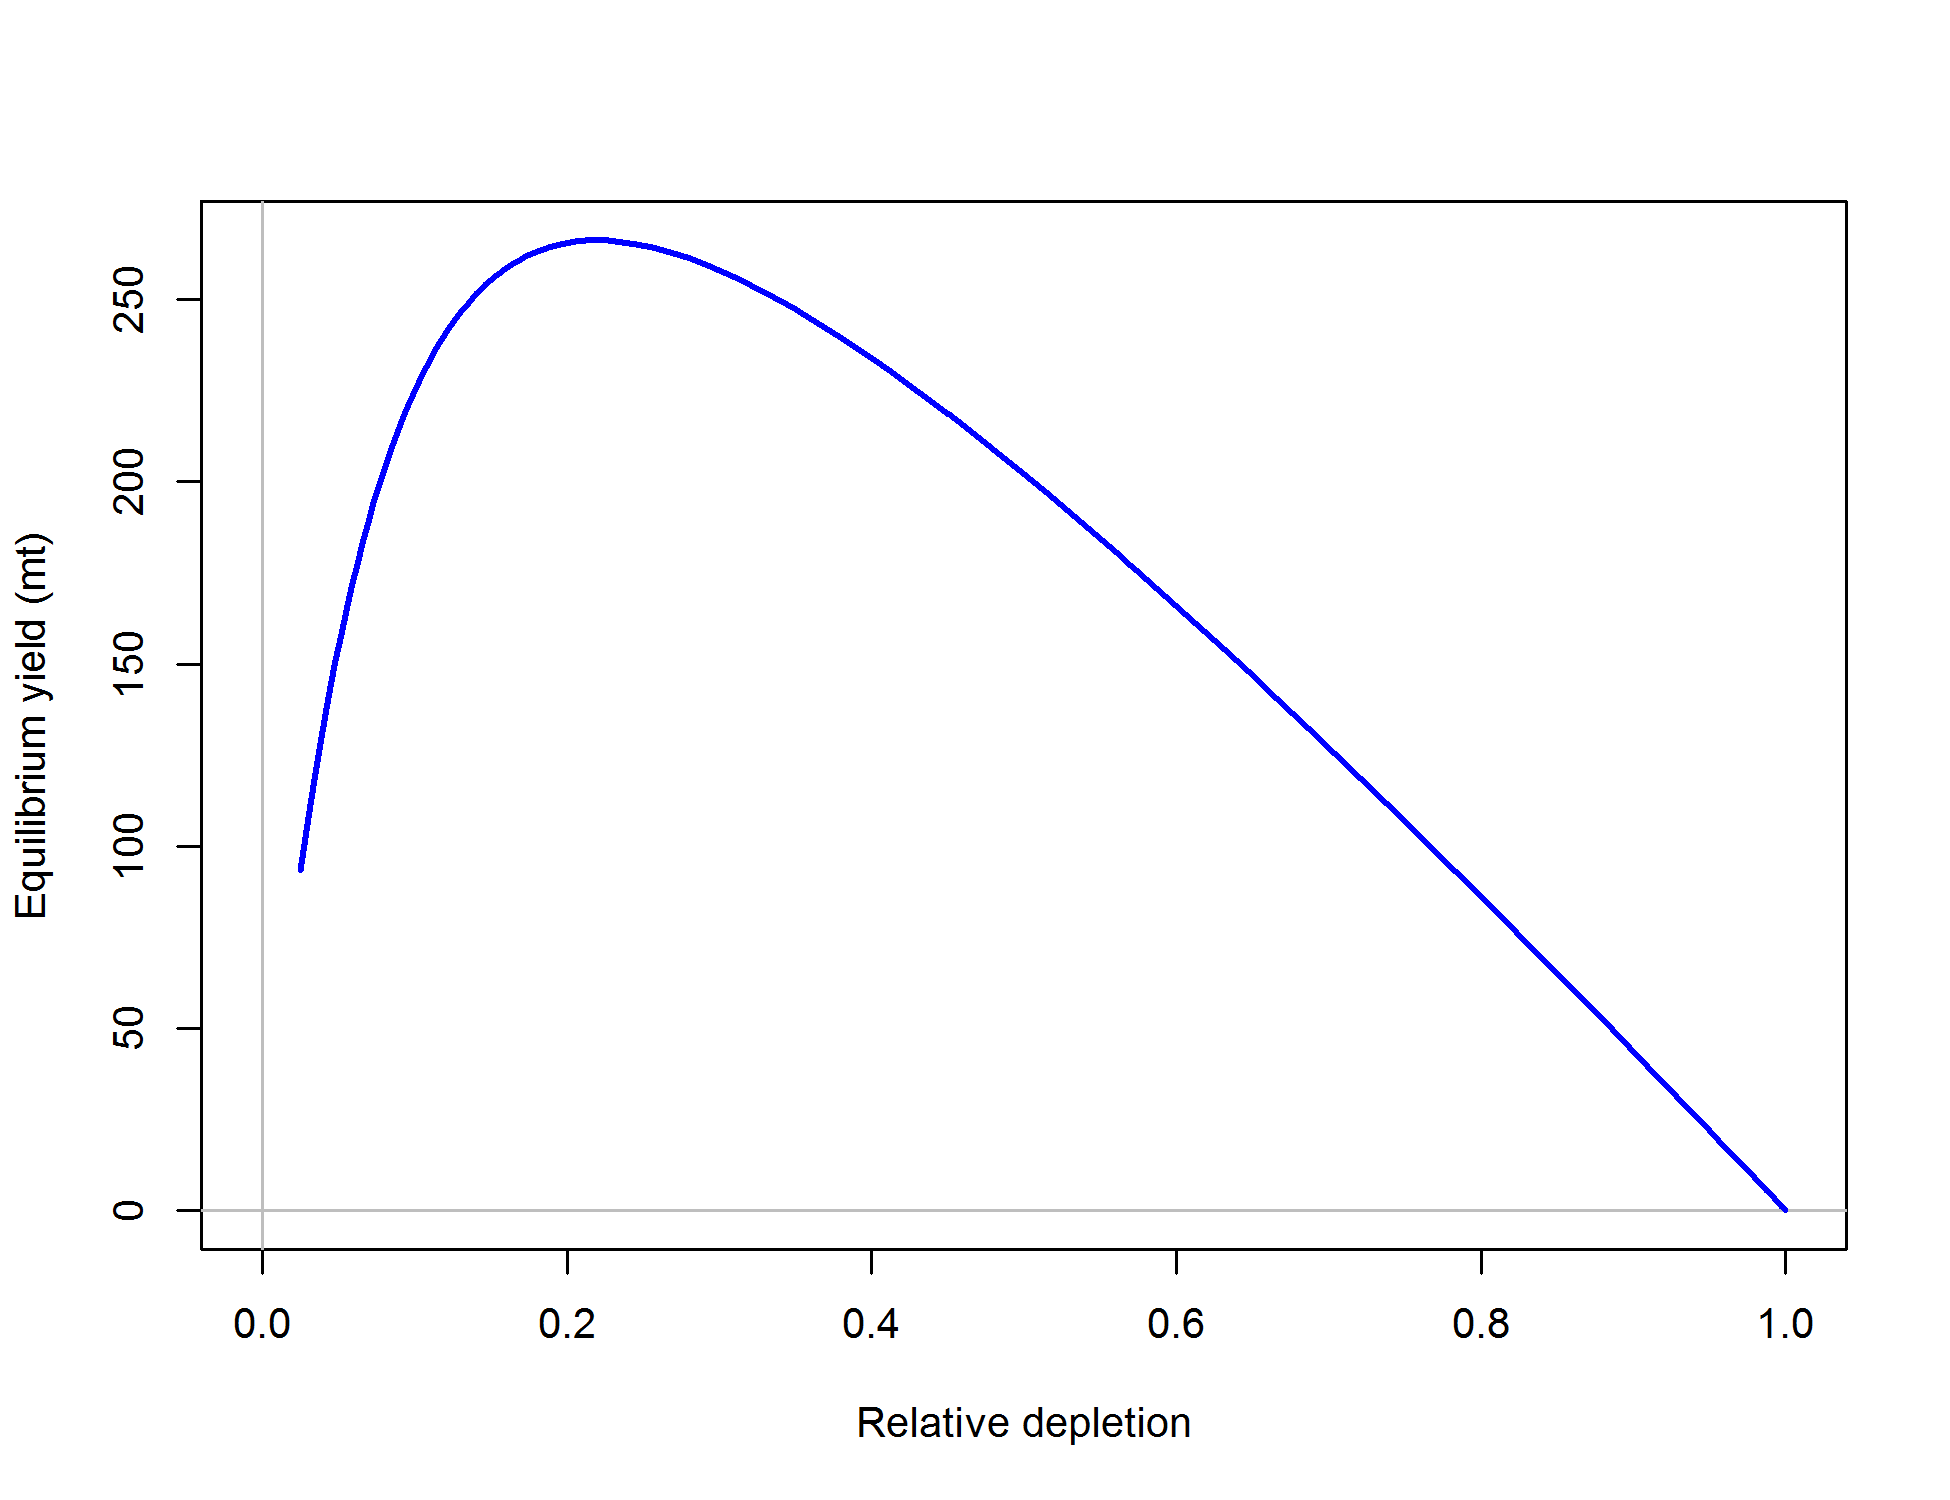
\includegraphics{r4ss/plots_mod1/yield1_yield_curve.png}
\caption{Equilibrium yield curve for the base case model. Values are
based on the 2016 fishery selectivity and with steepness fixed
at\ldots{} \label{fig:Yield_all}}
\end{figure}

\FloatBarrier

\newpage

\subsection*{Research And Data Needs}\label{research-and-data-needs}
\addcontentsline{toc}{subsection}{Research And Data Needs}

We recommend the following research be conducted before the next
assessment:

\begin{enumerate}

\item List item No. 1 in the list

\item List item No. 2 in the list, etc.

\end{enumerate}

\FloatBarrier

\newpage

\renewcommand{\thefigure}{\arabic{figure}}
\renewcommand{\thetable}{\arabic{table}}

\setcounter{figure}{0} \setcounter{table}{0}

\pagenumbering{arabic}

\section{Introduction}\label{introduction}

\subsection{Basic Information and Life
History}\label{basic-information-and-life-history}

California scorpionfish (\emph{Scorpaena guttata}), also known locally
as sculpin or spotted scorpionfish, originates from the Greek word for
scorpionfishes and \emph{guttata} is Latin for speckled. California
scorpionfish is a medium-bodied fish and like other species in the genus
\emph{Scorpaena}, it produces a toxin in its dorsal, anal, and pectoral
fin spines, which produces intense, painful wounds (Love et al.
\protect\hyperlink{ref-Love1987}{1987}). Scorpionfish are very resistant
to hooking mortality and have shown survival under extreme conditions.

Its range extends from central California (Santa Cruz) to the Gulf of
California, although within U.S. waters they are most common in the
Southern California Bight (Eschmeyer et al.
\protect\hyperlink{ref-Eschmeyer1983}{1983}, Love et al.
\protect\hyperlink{ref-Love1987}{1987}). The species generally inhabits
rocky reefs, caves and crevices, but in certain areas and seasons it
aggregates over sandy or muddy substrate (Frey
\protect\hyperlink{ref-Frey1971}{1971}, Love et al.
\protect\hyperlink{ref-Love1987}{1987}). California scorpionfish have
been observed from the intertidal to 600 ft with a preferred depth range
from 20-450 ft. Little is known about the aggregating behaviors of
California scorpionfish. Marine Applied Research and Exploration (MARE)
has observed California scorpionfish aggregations during the spawning
season (June 2014) and also in the late fall (November 2012) from video
transects in southern California. The November spawning aggregation was
observed at a small rocky feature near La Jolla and the June aggregation
was at a sandy area adjacent to the Farnsworth MPAs.

Males and females show different growth rates, with females growing to a
larger size than males, and the sexes exhibit different length-weight
relationships (Love et al. \protect\hyperlink{ref-Love1987}{1987}). Few
California scorpionfish are mature at one year old (14 cm total length).
Fifty-percent of fish mature at 17-18 cm (2 years old) and all by 22 cm
(4 years old) (Love et al. \protect\hyperlink{ref-Love1987}{1987}).

California scorpionfish feed on a wide variety of mobile prey, including
crabs, fishes (e.g., include northern anchovy, spotted cusk-eel),
octopi, isopods and shrimp, (Taylor
\protect\hyperlink{ref-Taylor1963}{1963}, Quast
\protect\hyperlink{ref-Quast1968}{1968}, Turner et al.
\protect\hyperlink{ref-Turner1969}{1969}, Love et al.
\protect\hyperlink{ref-Love1987}{1987}). The species is nocturnal, but
have been observed feeding during the day. Predation on scorpionfish is
believed to be low, but one individual was found in the gut of a leopard
shark (Love pers comm.).

\subsection{Early Life History}\label{early-life-history}

California scorpionfish utilize the ``explosive breeding assemblage''
reproductive mode in which fish migrate to, and aggregate at traditional
spawning sites for brief periods (Love et al.
\protect\hyperlink{ref-Love1987}{1987}). California scorpionfish migrate
to deeper waters (120-360 ft) to spawn during May-August, with peak
spawning occurring July. The species is oviparous, producing floating,
gelatinous egg masses in which the eggs are embedded in a single layer
(Orton \protect\hyperlink{ref-Orton1955}{1955}) and it is believed that
spawning takes place just before, and perhaps after dawn, in the water
column (Love et al. \protect\hyperlink{ref-Love1987}{1987}). The same
study tagged California scorpionfish and suggests individuals return to
the same spawning site, but information is not available on non-spawning
season site fidelity.

Little is known about California scorpionfish larvae. The CalCOFI survey
observed 463 California scorpionfish larvae from 1977-2000, with the
majority at station close to Oxnard (east of the Channel Islands) (Moser
et al. \protect\hyperlink{ref-Moser2002}{2002}). Higher densities of
larvae have been observed in the CalCOFI stations throughout Baja,
peaking south of Punta Eugenia from July to September. The hatching
length is reported as 1.9-2.0 mm (Washington et al.
\protect\hyperlink{ref-Washington1984}{1984}) and transformation length
of greater than 1.3 cm (Washington et al.
\protect\hyperlink{ref-Washington1984}{1984}) less than 2.1 cm (Moser
\protect\hyperlink{ref-Moser1996}{1996}).

\subsection{Map}\label{map}

A map showing the scope of the assessment and depicting boundaries for
fisheries or data collection strata is provided in Figure
\ref{fig:boundary_map}.

\subsection{Ecosystem Considerations}\label{ecosystem-considerations-1}

In this assessment, ecosystem considerations were not explicitly
included in the analysis.\\
This is primarily due to a lack of relevant data and results of analyses
(conducted elsewhere) that could contribute ecosystem-related
quantitative information for the assessment.

\subsection{Fishery Information}\label{fishery-information}

The hook-and-line fishery fishery off California developed in the late
19th century (Love et al. \protect\hyperlink{ref-Love2002}{2002}).\\
The rockfish trawl fishery was established in the early 1940s, when the
United States became involved in World War II and wartime shortage of
red meat created an increased demand for other sources of protein (Harry
and Morgan \protect\hyperlink{ref-Harry1961}{1961}, Alverson et al.
\protect\hyperlink{ref-Alverson1964}{1964}).

California scorpionfish comprise a minor part of the Californian sport
and commercial fisheries (Love et al.
\protect\hyperlink{ref-Love1987}{1987}). Historically, California
scorpionfish were taken commercially by hook and line and, occasionally,
by round haul nets (Daugherty
\protect\hyperlink{ref-Daugherty1949}{1949}). Scorpionfish were commonly
caught around Santa Catalina Island during the late 19th Century with
gillnets (Jordan \protect\hyperlink{ref-Jordan1887}{1887}). The 1937
Bureau of Commercial Fisheries report noted that California scorpionfish
had been a fairly important commercial species for a long time. The
species was targeted by a few fishermen during the summer months, and
was also taken as a bycatch in the rockfish fisheries. By 1949, Bureau
of Marine Fisheries reported\\
``{[}Scorpionfish{]} will even come to the surface to lights at night''
and were also taken in round haul nets. At that time, scorpionfish were
rarely targeted by fishermen except by a few specialists.

More recently, commercial bottom longlines have been used to target
spawning aggregations offshore of Long Beach (Love et al.
\protect\hyperlink{ref-Love1987}{1987}). Since the early 1990s, trawl
catch has been a substantial component of the commercial catch.
Commercial landings have fluctuated substantially over time, which
could, in part, be due to changes in targeting and El Niño events (Love
et al. \protect\hyperlink{ref-Love1987}{1987}). A high proportion of the
catch landed in California during the 1960s and 1970s was taken from
Mexican waters. In recent years, most of the catch has come from around
the Los Angeles region. In general, the majority of the commercial catch
has come from the Los Angeles region, except in the 1960s and 1970s when
the majority of the catch came from the San Diego region and Mexican
waters.

California scorpionfish is not a major target in the recreational
fishery. They are most often taken by boat fishermen, but fairly large
numbers are caught from piers, jettys, and rocky shorelines. The
Commercial Passenger Fishing Vessl (CPFV; also referred to as the
recreational party/charter or PC mode) effort has remained relatively
constant over a long period (1959-1998) (Dotson and Charter
\protect\hyperlink{ref-Dotson2003}{2003}). However, there appears to be
a shift in effort towards less utilized species, such as California
scorpionfish, over the past decade (Dotson and Charter
\protect\hyperlink{ref-Dotson2003}{2003}). Especially as catch limits
for rockfish have become more restricted commercial passenger fishing
vessels (CPFV) operators target California scorpionfish spawning
aggregations during spring and summer (Love et al.
\protect\hyperlink{ref-Love1987}{1987}), and also target California
scorpionfish in the winter when other fisheries are closed.\\
California scorpionfish become a target species for day boats during the
spawning months when spawning aggregations can be located. There are a
small number of boats that specialize in targeting these aggregations.
The spawning aggregations occur in deeper waters, often times outside of
the three nautical mile state jurisdiction. It is also unknown what
fraction of the population aggregates during the spawning season, e.g.,
all mature fish.

Aggregate mortality has been far below the Annual Catch Limits (ACL)
established by the 2005 stock assessment. The ACL projections from the
2005 assessment assumed that the entire ACL was being taken each year
and as a result, the ACL for each subsequent year declined despite
under-attainment in reality.\\
In addition, in 2014, recreational catch was higher than expected. As a
result, in 2014, the combined recreational and commercial catch exceeded
the OFL by 2mt (1\%) resulting from assumption that the ACL had been
attained. Subsequently, action was taken to decrease the recreational
season by four months (September 1 - December 31). A catch only update
of the stock was undertaken in 2015 (Wallace and Budrick
\protect\hyperlink{ref-Wallace2015}{2015}) that imputed the actual catch
values since the last assessment, resulting in significant increase in
the OFL and ACL.\\
Retrospectively, the catch in 2014 was well below the OFL as well as the
ACL that would have been in place had the ACL values from the actual
attainment been in place in 2014. Thus the stock has not been subject to
overfishing since the original assessment or been in an overfished
condition historically and is considered healthy.\\
The season restriction in the recreational fishery remained in place as
a precautionary measure until the full assessment is completed to better
inform the current status of the stock, catch limits and regulations
given the perspective provided.

\subsection{Summary of Management
History}\label{summary-of-management-history}

Prior to the adoption of the Pacific Coast Groundfish Fishery Management
Plan (FMP) in 1982, California scorpionfish (\emph{Scorpaena guttata})
was managed through a regulatory process that included the California
Department of Fish and Wildlife (CDFW) along with either the California
State Legislature or the Fish and Game Commission (FGC) depending on the
sector (recreation or commercial) and fishery. With implementation of
the Pacific Coast Groundfish FMP, California scorpionfish came under the
management authority of the Pacific Fishery Management Council (PFMC),
being incorporated, along with all genera and species of the family
Scorpaenidae, into a federal rockfish classification and managed as part
of ``Remaining Rockfish'' under the larger heading of ``Other Rockfish''
(PFMC (\protect\hyperlink{ref-PFMC2002}{2002},
\protect\hyperlink{ref-PFMC2004}{2004}), Tables 31-39).

The ABCs provided by the PFMC's Groundfish Management Team (GMT) in the
1980's were based on an analysis of commercial landings from the 1960's
and 1970's. For this analysis, most of the rockfishes were lumped into
one large group. This analysis indicated that the landings for rockfish
in the Monterey-Conception area were at or near ABC levels (Pacific
Fishery Management Council \protect\hyperlink{ref-PFMC1993}{1993}). To
keep landings within these adopted harvest targets, the Pacific Coast
Groundfish FMP provided the Council with a variety of management tools
including area closures, season closures, gear restrictions, and, for
the commercial sector, cumulative limits (generally for two-month
periods). With the implementation of a federal groundfish restricted
access program in 1994, allocations of total catch and cumulative limits
began to be specifically set for open access (including most of
California's commercial fisheries that target California scorpionfish in
Southern California) and limited entry fisheries (Pacific Fishery
Management Council \protect\hyperlink{ref-PFMC2002}{2002},
\protect\hyperlink{ref-PFMC2004}{2004}). As a result, in the later
1990'ss as commercial landings decreased and recreational harvest became
a greater proportion of the available harvest.

Beginning in 1997, California scorpionfish was managed as part of the
Sebastes complex-south, Other Rockfish category. (\emph{Sebastes}
complex-south included the Eureka, Monterey, and Conception areas while
Sebastes complex-north included the Vancouver and Columbia areas.) The
PFMC's rockfish management structure changed significantly in 2000 with
the replacement of the \emph{Sebastes} complex -north and -south areas
with Minor Rockfish North (now covering the Vancouver, Columbia, and
Eureka areas) and Minor Rockfish South (now Monterey and Conception
areas only). The OY for these two groups (which continued to be
calculated as 0.50 of the ABC) was further divided (between north and
south of \(40^\circ 10^\prime\) N. latitude) into nearshore, shelf, and
slope rockfish categories with allocations set for Limited Entry and
Open Access fisheries within each of these three categories (January 4,
2000, 65 FR 221; PFMC (\protect\hyperlink{ref-PFMC2002}{2002}), Tables
54-55). Because of its depth range and southern distribution, California
scorpionfish was included within the Minor Rockfish South, Other
Rockfish ABC and managed under the south of \(40^\circ 10^\prime\) N.
latitude nearshore rockfish OY and trip limits (PFMC
(\protect\hyperlink{ref-PFMC2002}{2002}), Table 29).

Along with the above changes, in 2000 the southern area divided into two
separate management areas at Point Lopez, \(36^\circ 00^\prime\) N.
latitude. This was followed in 2001 with the implementation of the
northern rockfish and lingcod management area between
(\(40^\circ 10^\prime\) N. latitude) and Point Conception
(\(34^\circ 27^\prime\) N. latitude); and the southern rockfish and
lingcod management area between Point Conception and the U.S.- Mexico
border. These were later revised starting in 2004 with the northern
rockfish and lingcod management area redefined as ocean waters from the
Oregon-California border (\(42^\circ 00^\prime\) N. latitude) to
\(40^\circ 10^\prime\) N. latitude, the central rockfish and lingcod
management area defined as ocean waters from \(40^\circ 10^\prime\) N.
latitude to Point Conception, and the southern rockfish and management
area continuing to be defined as ocean waters from Point Conception to
the U.S.-Mexico border.

Cowcod Conservation Areas (CCAs) also were established in 2001 to reduce
fishing effort in areas with high encounter rates of cowcod rockfish
(PFMC (\protect\hyperlink{ref-PFMC2002}{2002}), Table 29). These areas
were closed to all recreational and commercial fishing for groundfish
except for minor nearshore rockfish1 (including California scorpionfish)
within waters less than 20 fathoms. The California Rockfish Conservation
Area (CRCA) was defined as those ocean waters south
\(40^\circ 10^\prime\) N. latitude to the U.S.-Mexico border with
different depth zones specified for the areas north and south of Pt.
Reyes (\(37^\circ 59.73^\prime\) N. latitude).

During the late 1990's and early 2000's, major changes also occurred in
the way that California managed its nearshore fishery. The Marine Life
Management Act (MLMA), which was passed in 1998 by the California
Legislature and enacted in 1999, required that the FGC adopt an FMP for
nearshore finfish. It also gave authority to the FGC to regulate
commercial and recreational nearshore fisheries through FMPs and
provided broad authority to adopt regulations for the nearshore fishery
during the time prior to adoption of the nearshore finfish FMP. Within
this legislation, the Legislature also included commercial size limits
for nine nearshore species including California scorpionfish (10-inch
minimum size) and a requirement that commercial fishermen landing these
nine nearshore species possess a nearshore permit.

Following adoption of the Nearshore FMP and accompanying regulations by
the FGC in fall of 2002, the FGC adopted regulations in November 2002
which established a set of marine reserves around the Channel Islands in
Southern California (which became effective April 2003). The FGC also
adopted a nearshore restricted access program in December 2002 (which
included the establishment of a Deeper Nearshore Permit) to be effective
starting in the 2003 fishing year.

Although the Nearshore FMP provided for the management of the nearshore
rockfish and California scorpionfish, management authority for these
species continued to reside with the Council. Even so, for the 2003 and
subsequent fishery seasons, the State provided recommendations to the
Council specific to the nearshore species that followed the directives
set out in the Nearshore FMP. These recommendations, which the Council
incorporated into the 2003 management specifications, included a
recalculated OY for Minor Rockfish South - Nearshore, division of the
Minor Rockfish South - Nearshore into three groups (shallow nearshore
rockfish; deeper nearshore rockfish; and California scorpionfish), and
specific harvest targets and recreational and commercial allocations for
each of these groups.

Also, since the enactment of the MLMA, the Council and State in a
coordinated effort developed and adopted various management
specifications to keep harvest within the harvest targets, including
seasonal and area closures (e.g.~the CCAs; a closure of Cordell Banks to
specific fishing), depth restrictions, minimum size limits, and bag
limits to regulate the recreational fishery and license and permit
regulations, finfish trap permits, gear restrictions, seasonal and area
closures (e.g.~the RCAs and CCAs; a closure of Cordell Banks to specific
fishing), depth restrictions, trip limits, and minimum size imits to
regulate the commercial fishery.

\subsection{Management Performance}\label{management-performance-1}

Management performance table: (Table \ref{tab:mnmgt_perform})\\
A summary of these values as well as other base case summary results can
be found in Table \ref{tab:base_summary}.

\subsection{Fisheries off Mexico}\label{fisheries-off-mexico}

The California scorpionfish's range extends into to Abreojos, Baja
California.\\
The species is also found in the northern Gulf of California and
Guadalupe Island. No formal stock assessments have been conducted for
California scorpionfish in Mexican waters.

\section{Assessment}\label{assessment}

\subsection{Data}\label{data}

Data used in the California scorpionfish assessment are summarized in
Figure \ref{fig:data_plot}.\\
A description of each data source is below.

\subsubsection{Commercial Fishery
Landings}\label{commercial-fishery-landings}

Commercial catches of California scorpionfish (often landed as
``sculpin'') are available back to 1916. Landings from 1916 to 1935 are
presented in CDFG Fish Bulletin No. 49 and Bulletin No. 149 provides
tabulated data from 1916 to 1968. Over 99\% of the commercial catches of
California scorpionfish are from south of Pt. Conception.\\
Whenever possible, catches from north of Pt. Conception and also caught
in Mexico but landed in the U.S. were excluded from the commercial catch
histories.

\href{http://library.ucsd.edu/ceo/fishcatchtables/fish-catch-download.html}{California
Explores the Ocean}(CEO) provides landings data taken from the CDFG Fish
Bulletins in electronic form, as well as electronic copies of all CDFG
Fish Bulletins.

Statewide annual landings are available for California scorpionfish from
1916 to 1925, and are assumed to be taken by hook-and-line. Data by area
and month are given in a series of bulletins, each bulletin usually
providing information for a single year. Data by region and month is
available for 1926 to 1986. The Santa Barbara region includes San Luis
Obispo, Santa Barbara and Ventura counties. Catches from this region
were included in the catch history and comprised less than 10 mt for the
period from 1926-1968 (the period when data at the regional scale are
available).\\
Catches from Mexico can be separated from the total catch starting in
1931, although the CDFG Bulletins do not report catches originating from
Mexican waters available for all years, e.g., 1932-1934. It is assumed
that before 1931 there was no catch taken from Mexican waters landed in
California.

The \href{http://128.114.3.187/}{CALCOM} database was queried (March 7,
2017) for commercial landing estimates of California scorpionfish in
California, 1969-2016. Landings were stratified by year, quarter,
live/dead, market category, gear group, port complex, and source of
species composition data (actual port samples, borrowed samples, or
assumed nominal market category). All CALCOM California scorpionfish
landing data are either actual port samples or the nominal California
scorpionfish market category. However, catches in CALCOM do not separate
out catches originating from Mexican waters and landed at U.S. ports.

The Commercial Fisheries Information System (CFIS; maintained by CDFW)
contains California catch in pounds by gear and port for 1969 to 2016
(Figures). The CFIS data come from landing receipts or ``fish tickets''
filled out by the markets or fish buyers as required by the state for
all commercial landings. The fish tickets include the CDFW block in
which the majority of the landings were caught.\\
Landings with a block solely in Mexican waters (blocks
\textgreater{}900) were removed from the catch history. Landings with
reported blocks 877-882 with area in both U.S. and Mexican waters were
retained in the catch histories. The commercial catch is dominated by
the hook-and-line fishery (89\% of total catches).\\
The catch by reported gear types: hook-and-line, fish pot, trawl, gill
net, and other can be found in Table \ref{tab:CommCatches}. Catch taken
by fish pot and other gears is added to the hook-and-line catch in the
stock assessment (30.6 mt from fish pot and 93.9 mt from other gears).

In the assessment, catch for 1916 to 1968 is taken from the CDFG Fish
Bulletins. Catch by gear for 1969 to 2004 is taken from CFIS.

\subsubsection{Commercial Discards}\label{commercial-discards}

Information on commercial discards from the West Coast Groundfish
Observer Program (WCGOP) are available starting in 2004. The commercial
fishery for California scorpionfish has been minimal since the early
2003 (averaging 3.5 mt per year). The available length composition data
from the observed discards is minimal, with 151 fish measured from
2004-2015, and less than half a metric ton. Given the discard mortality
of only 7\%, and the small total catches in the recent years, discards
from the commercial fleet are not considered in the assessment.

\subsection{Commercial Fishery Length And Age
Data}\label{commercial-fishery-length-and-age-data}

Biological data from commercial fisheries that caught California
scorpionfish were extracted from CALCOM on March 7, 2017. Samples from
the hook and line fishery were available from 1999 (1 trip) and
2013-2015 (1 trip per year), and for 1999 (1 trip) and 2006 (2 trips)
from the trawl fishery. A total of 87 fish were measured and length
compositions were based on expanded catch-weighted landings. The samples
from 1999 for both fisheries were replaced by samples from the market
category study described below.

The CDFW conducted a market study from 1990-2004 in southern California
(Laughlin and Ugoretz \protect\hyperlink{ref-Laughlin1998}{1998}) to
monitor and summarize local commercial catches. The ports sampled
included San Diego, Santa Barbara/Ventura and Long Beach/San Pedro. Very
few of the samples from Santa Barbara and San Diego (4 samples each from
the hook-and-line and trawl fisheries Santa Barbara, and 1 sample from
the hook-and-line fishery in San Diego) reported California
scorpionfish, and are excluded from the length composition data.\\
Length composition for California scorpionfish are available from the
Long Beach samples for the hook-and-line (Table
\ref{tab:ComHL_lengthsample}), gillnet (Table
\ref{tab:ComNet_lengthsample}), and trawl fisheries (Table
\ref{tab:ComTrawl_lengthsample}). Length samples from both groundfish
(otter) trawls and single-rigged shrimp trawls were available from the
market study. The average size of fish from the otter trawls (26.5 cm)
was smaller than from the shrimp trawl samples (28.1 cm). Over 70\% of
California scorpionfish catch from the trawl sector was landed from
single-rigged shrimp trawls, which best represent the length composition
of the trawl fleet (CALCOM).

The input sample sizes were calculated via the Stewart Method (Ian
Stewart, personal communication, IPHC):

\begin{centering}

Input effN = $N_{\text{trips}} + 0.138 * N_{\text{fish}}$ if $N_{\text{fish}}/N_{\text{trips}}$ is $<$ 44

Input effN = $7.06 * N_{\text{trips}}$ if $N_{\text{fish}}/N_{\text{trips}}$ is $\geq$ 44

\end{centering}

\subsubsection{Sport Fishery Removals and
Discards}\label{sport-fishery-removals-and-discards}

Data used in reconstructing the retained catch and discarded mortality
for California scorpionfish in the California recreational fishery are
from the Commercial Passenger Fishing Vessel (CPFV) Logbooks
(1932-2017), the Marine Recreational Fishery Statistical Survey (MRFSS,
1980-2003) and the California Recreational Fishery Survey (CRFS,
2004-2017).\\
Total catch was accounted for including retained catch as well as the
estimate of fish discarded dead assuming a 7\% discard mortality rate
approved for use in management in the regulatory specifications for
2009-2010 (Pacific Fishery Management Council
\protect\hyperlink{ref-PFMC2008}{2008}). The MRFSS and CRFS data provide
estimates of mortality for four fishing ``modes'' including the
Party/Charter Boat, Private/Rental Boat, Man Made (piers and jetties
etc.) and Beach and Bank modes.

While estimates of mortality from the Party/Charter (PC) boat mode is
available from the MRFSS and CRFS surveys for the Party/Charter Boat
mode for 1980-2017, estimates from the CRFS data from 2011-2017 and data
from CPFV Logbook for 1932-2010 were used to represent catch from this
mode. The Party/Charter Phone Survey was used to estimate effort used in
producing effort estimates for CRFS between 2004 and 2010, which was
subject to negative bias due to the low of participation in the survey
south of Point Conception. The Coastal County Household Telephone Survey
was used to estimate fishing effort for the MRFSS survey from 1980-2003
and was subject to potential positive avidity bias in participation by
those contacted by the survey. As a result, the CPFV logbooks provided
the reported number of retained and discarded California scorpionfish
used to estimate mortality from 1932-2010.\\
This is consistent with the catch based update conducted in 2015 as well
as the original assessment, both of which used estimates of catch from
logbooks to represent catch in the PC mode with the exception of the
years after 2011 when effort estimates used in CRFS estimates were
derived from logbooks.

An under-reporting adjustment reflecting an average 20\% of logs not
being submitted was applied to all estimates for the PC mode from
1932-2010. Annual average weights from this mode for retained catch from
the MRFSS or CRFS estimates for 1980-2010 and average weight from
1980-1984 was applied to the preceding years. To estimate discard
mortality for the PC mode, the annual average weight was applied in
respective years from lengths collected sampling onboard CPFVs by the
CRFS survey for 2004-2010 were applied to the number of discards from
the CPFV logbooks and the average weight over this entire period were
applied to the preceding years for 1995-2003. For the period between
1980 and 1994, the MRFSS estimates for discards were used to reflect
discarding due to the paucity of data on the number of discards from PC
logbooks prior to 1995.

For all other modes, the MRFSS (1980-2003) and CRFS (2004-2017) based
estimates of retained catch and discard mortality were used. There was a
lapse in MRFSS sampling from 1990 through 1992, for which retained catch
and discard mortality were estimated using the average of values three
years before and three years after the lapse for all modes other than
the PC mode. For the PC mode, estimates of numbers of fish were
available from logbook data and average weight from the three years
before and after this period were applied to provide estimates for the
PC mode.

Estimates of retained catch and discards were not available from the
non-PC modes prior to 1980, thus the ratio of catch in the PC mode to
the other modes for 1980 through 1985 was used to provide an estimate of
catch in the other modes in the years 1932-1979. In the case of the PR
mode, a linear ramp in the ratio adjustment between PC and PR modes was
applied between 1966 and 1979 from 0.55 in 1980 to 0.10 in 1965,
reflecting the increase in the relative proportion of catch contributed
by the PR mode with time as more individuals anglers purchased vessels,
as recommended in the California Catch Reconstruction (Ralston et al.
\protect\hyperlink{ref-Ralston2010}{2010}), and the ratio of 0.10 was
assumed for all years prior. The ratio of PC estimates to the MM and BB
modes was assumed to constant and the average between 1980 and 1989 was
applied from 1932 to 1979. Catch estimates from CPFV logbooks were not
available during the World War II era from 1941 until 1946 and catch was
assumed to be zero for all modes during this period. Estimates for
retained catch and discarded mortality for 1935 to 1928 were estimated
using a linear ramp from the value for 1928 to zero in 1936 for the PC
mode and ratios PC compared to other modes were used to proxy estimates
for other modes based on the resulting ramped values for the PC mode.
The final time series of landings and discard mortality are in Table
\ref{tab:Rec_removal}.

Biological samples from the recreational fleets are desired in the
sections below.

\subsubsection{Fishery-dependent Data
Sources}\label{fishery-dependent-data-sources}

\textbf{CRFS Private Boat Dockside Intercept Survey}

The CDFW provided the CRFS private boat dockside sampling fisheries data
from 2004 to 2016. The data went through several data quality checks to
identify the best subset of available data that are consistent over the
time series and provide a representative relative index of abundance
once standardized. The dockside sampling of the private mode (PR mode in
RecFIN) consists of samples from a primary series of ports (PR1) where
the majority of fishing effort for this mode originates and a secondary
series of ports with historically low effort (PR2). Only PR1 samples
were used for this index as the sampling forms for the PR2 index have
changed over time and the data could not reliably be collapsed to the
trip level. The dockside data consist of two types of data; Type 2 data
contain records of angler-reported catch, i.e., catch that was not
observed by the sampler and Type 3 data includes sampler-examined
retained catch. Of the Type 2 reported catch for scorpionfish, less than
one percent were reported ``thrown back dead'' and five percent reported
as retained to eat. Given that the reported retained catch is a small
fraction of the catch overall and discard mortality of California
scorpionfish is low, only the Type 3 examined catch are used in the
index.

The survey records the number of contributing anglers (number of anglers
on the vessel for the private mode), but does not contain data on hours
fished. For this index, angler-day was the assumed effort. The data were
filtered to trips fishing with hook-and-line gear in southern
California. Trips with a primary fishing area of Mexico were also
removed. The CRFS dockside private boat records with these broad filters
include 44,128 trips of which 3,802 caught California scorpionfish
(8.6\%).

The Stephens-MacCall approach was used to identify trips with a high
probability of catching California scorpionfish (Stephens and MacCall
\protect\hyperlink{ref-Stephens2004}{2004}). Prior to using the
Stephens-MacCall approach to select relevant trips a number of other
filters were applied to the data to minimize variability in CPUE
estimates. Over the course of the time series only 45 trips from Santa
Barbara county encountered California scorpionfish, ranging from 0-10
trips a year. The Stephens-MacCall approach was applied with and without
trips from Santa Barbara and the same species were identified as
indicators and counter-indicators. For the final model prior to
Stephens-MacCall, trips from Santa Barbara were excluded, leaving 41,235
trips, and 3,747 of those caught California scorpionfish (Table
\ref{tab:Fleet4_RecPR_dockside_filter}).

Coefficients from the Stephens-MacCall analysis (a binomial GLM) are
positive for species which co-occur with California scorpionfish, and
negative for species that are not caught with California scorpionfish
(Figure \ref{fig:Fleet4_RecPR_dockside_SM}). Potentially informative
species for the Stephens-MacCall analysis were limited to species caught
in at least one percent of all trips and caught in at least five years.
Some of these never occurred with California scorpionfish (strong
`counter-indicators') and records with these species were removed from
the data prior to estimation of the index. Strong counter-indicators for
the CRFS private boat index included yellowfin tuna and dolphinfish.

A total of 8,590 trips were retained following the Stephens-MacCall
filter, with 3,056 all positive California scorpionfish trips retained.
The California scorpionfish recreational fishery in the southern
management area was closed for eight months in 2004 and nine months in
2005. The majority of records from 2004 and 2005 are from the period
when the fishery was closed and were removed from the analysis (Figure
\ref{fig:recregs}). Records from months with the fishery was closed from
2006-2016 were also excluded from the index since this index relies on
sampler-examined retained catch.

Catch per unit effort was modeled using a delta-GLM approach, where the
catch occurrence (binomial) component was modeled using a logit link
function and the positive catch component was modeled after
log-transformation of the response variable, according to a normal
distribution with an identity link function. The units for CPUE are fish
landed/anglers. A gamma distribution for the positive catch component
was also explored, but model selection favored the lognormal model. The
raw CPUE of factors considered in the model by year are shown in Figure
\ref{fig:Fleet4_RecPR_dockside_lograwCPUE}.

Model selection procedures selected the covariates \emph{2-month wave}
and \emph{county} as important for both the catch occurrence and
positive catch component models for all data sets, along with the
categorical year factor used for the index of abundance (Table
\ref{tab:Fleet4_RecPR_dockside_aic}).\\
The Q-Q goodness of fit plot for the lognormal portion of the model
shows a moderate fit to the data (Figure
\ref{fig:Fleet4_RecPR_dockside_QQ}). final index indicates a decrease in
relative abundance from 2006 to 2010, at which point the index is
relatively flat (Figure \ref{fig:index5_logcpuefit_RecPR}).

Biological samples from trips retaining California scorpionfish were
collected during the dockside surveys. Lengths of California
scorpionfish from 1980-2016 for the private mode were provided by RecFIN
by Edward Hibsch (PSMFC) on November 29, 2016. Length measurements from
the private mode were provided directly from CDFW for the years
2004-2016 Table \ref{tab:Fleet4_lengthsample}. The number of trips is
the number of unique ID\_CODEs from RecFIN for 1980-2003. Starting in
2004 with the CRFS program, the number of unique trips sampled in the
private boat mode was recorded. The recreational private fleet tends to
select larger fish than the recreational party/charter fleet, which is
one reason the private and party/charter fleets were maintained as two
separate fleets in the base model. No length data for discarded fish
from the recreational private mode fleet are available.

\textbf{CRFS CPFV Logbook Index}

CPFV operators have been required to submit written catch logs with
daily trips records of catches to CDFW since 1935. The logbook data from
1936-1979 are available as monthly summaries, which do not contain the
level of detail needed for an index of abundance. CDFW provided the CPFV
logbook data from 1980-2016 (Charlene Calac, CDFW). Logbook data from
1980-2016 contain records for each trip, including the fishing date,
port of landing, vessel name and number, CDFG block area fished (Figure
\ref{fig:boundary_map}), angler effort, number of fish kept and
discarded by species. As of 1994, operators were required to report the
number of fish discarded and lost to seals. Prior to 1994, it is assumed
that all reported fish were retained. Details and additional information
on the historical logbook database can be found in Hill and Schneider
(\protect\hyperlink{ref-Hill1999}{1999}).

The number of anglers on board the vessel and the hours fished are
included in the database for all years. Only retained fish are included
in the index of abundance the unit of effort is angler hours. A number
of data filters were applied to the data to account for possible
mis-reporting, e.g., trips reporting retained California scorpionfish in
top 1\% of the data (\textgreater{}325 fish). Trips fishing outside of
California scorpionfish habitat (reported as targeting pelagic species)
or trips reporting a block with a minimum depth deeper than 140 m were
also filtered out.

Because California scorpionfish is not a primary target species, boats
with fewer than 10 trips retaining California scorpionfish were removed
from the analysis. Data were also filtered to only include catches
reported from blocks South of Pt. Conception and north of the
U.S.-Mexico border (Figure \ref{fig:boundary_map}), and blocks with at
least 100 trips retaining California scorpionfish and a total of 500
trips. A full description of the data filters is in Table
\ref{tab:Fleet5_RecPC_CPFVlogbook_filter}. A total of 432,868 trips were
retained for the index of abundance, 202,937 of which caught California
scorpionfish.

Two different area factors were considered for the standardization,
block and region.\\
The 60 retained blocks were split into nearshore regions north and south
of San Pedro and the northern and southern islands, for four regions.
Both a delta model and a negative binomial model were considered for
index standardization. However, due to the large number of records, the
traditional jackknife routine to estimate uncertainty was not possible.

California scorpionfish were present in 47\% of all trips, and
standardized with a negative binomial model. Factors considered were
\emph{year}, \emph{month}, and \emph{area} (either block or region). A
model with blocks and was selected over a model with region by 39,180
AIC. The final model includes \emph{year}, \emph{month}, and
\emph{block} with a log link and effort as an offset (Table
\ref{tab:Fleet5_RecPC_CPFVlogbook_aic}).\\
The standardized index shows a cyclic pattern, with period of higher
CPUE (late 1980's to early 1990's and late 1990s) and has shown a
general downward trend since 2008 (Figure
\ref{fig:index5_logcpuefit_RecPC}). An interesting note is the
similarity in standardized CPUE between the CPFV logbook index and the
CPFV dockside index (not used in the stock assessment model) from
1992-1997 (for a Stephens-MacCall threshold of 0.1) (Figure
\ref{fig:Fleet5_RecPC_dockside_index_compare}).

\textbf{MRFSS Party/Charter Boat Dockside Index}

From 1980 to 2003 the MRFSS program sampled landings at dockside (called
an ``intercept'') upon termination of recreational fishing trips. The
program was temporarily suspended from 1990-1992 due to lack of funding.
For purposes of this assessment, the MRFSS time series is truncated at
1998 due to overlap with an alternative index used to represent 1999
onward using onboard sampling data making analysis using the dockside
data redundant (see ``Recreational Onboard Observer Surveys''). Only
trips south of Point Conception were included in the analysis as
California scorpionfish are exceedingly uncommon in the catch to the
north. The California party and charter boat (a.k.a. ``PC mode,''
commercial passenger fishing vessel, or CPFV) samples used in the
present analysis provide catch and effort data aggregated at the trip
level. Each entry in the RecFIN Type 3 database corresponds to a single
fish examined by a sampler at a particular survey site. Since only a
subset of the catch may be sampled, each record also identifies the
total number of that species possessed by the group of anglers being
interviewed. The number of anglers and the hours fished are also
recorded. Unfortunately the Type 3 data do not indicate which records
belong to the same boat trip. Because our aim is to obtain a measure of
catch per unit effort (fish per angler hour), it is necessary to
separate the records into individual trips. For this reason trips must
be inferred from the RecFIN data. This is a lengthy process, and is
outlined in Supplemental Materials (``Identifying Trips in RecFIN'').

Since recreational fishing trips target a wide variety of species,
standardization of the catch rates requires selecting trips that are
likely to have fished in habitats containing California scorpionfish.
The method of Stephens and MacCall
(\protect\hyperlink{ref-Stephens2004}{2004}) was used to identify trips
with a high probability of catching California scorpionfish, based on
the species composition of the catch in a given trip. Prior to applying
the Stephens-MacCall filter, we identified potentially informative
``predictor'' species , i.e., those with sufficient sample sizes and
temporal coverage (at least 30 positive trips total, distributed across
at least 10 years of the index) to inform the binomial model.
Coefficients from the Stephens-MacCall analysis (a binomial GLM) are
positive for species which co-occur with California scorpionfish, and
negative for species that are not caught with California scorpionfish.

Data for dockside sampling of 6,295 commercial passenger fishing vessel
(CPFV) trips south of Point Conception by the Marine Recreational
Fishery Statistical Survey (MRFSS) were filtered using the
Stephens-McCall method to identify trips with catch associated with
California scorpionfish and the resulting trips analyzed in a delta-GLM
including year and county to produce annual indices of abundance for the
period 1980 through 1998 . To eliminate trips targeting species caught
near the surface for all or part of the trip where California
scorpionfish do not occur, prior applying the Stephens-MacCall filter,
trips with catch of bluefin tuna, yellowfin tuna, dorado, Pacific
bonito, skipjack, albacore, chinook salmon, coho salmon and bigeye tuna
were removed. Trips with catch of yellowtail amberjack were also removed
since effort on such trips can often be focused in the surface and
mid-water where California scorpionfish do not occur. In addition, trips
with aggregate effort less below and above 95\% percentile (less than 2
and over 109.5 hours) were removed to exclude trips for which either too
little effort was exerted to be informative or longer trips that may
make an excessive contribution to the effort likely distributed over a
number of targets only some of which may co-occur with California
scorpionfish biasing low the resulting CPUE. Lastly, trips in Santa
Barbara County were removed due the low number of positive samples for
California scorpionfish since it resides in the northern extent of their
range and this is a transition zone between biogeographic provinces in
which the presence of more northerly distributed species could adversely
affect the ability of the Stephens-MacCall filtering method to identify
co-occurring species. Each of these filtering steps and the resulting
number of trips remaining in the sampling frame are provided in Table
\ref{tab:Fleet5_RecPC_dockside_filter}.

Removal of the aforementioned trips resulted in a total of 3,968 trips
to which the Stephens-MacCall filtering method was applied. Species that
composed less than 5\% of the catch were excluded from analysis to
prevent these uncommon species from affecting correlations identified
using the algorithm. Chub mackerel, Pacific mackerel and barracuda were
removed as potential predictor species despite having weak positive
correlations with California scorpionfish since they are predominantly
pelagic and their co-occurrence is not expected to be predictive. As
expected, positive indicators of California scorpionfish trips include
several species of nearshore rockfish, California sheephead, California
halibut, Pacific sanddabs and seabasses and counter-indicators include
several species of deep-water rockfish (Figure
\ref{fig:Fleet5_RecPC_docksideSM}). While the filter is useful in
identifying co-occurring or non-occurring species assuming all effort
was exerted in pursuit of a single target, the targeting of more than
one target species can result in co-occurrence of species in the catch
that do not truly co-occur in terms of habitat associations informative
for an index of abundance, presenting a confounding influence in
selecting trips using the methods employed. Thus the filtering is
intended to remove those trips for which effort was targeted in deeper
water than California scorpionfish commonly occur.

Two levels of filtering were applied using the Stephens-MacCall Filter.
The Stephens-MacCall filtering method identified the probability of
occurrence (in this case 0.27) at which the rate of false positives and
false negatives for the presence of California scorpionfish were equal
as a heuristic for selecting a threshold for trips in appropriate
habitat to be included in analysis. The trips from this criteria for
selection was compared to an alternative method including the false
positive trips as well as all positive trips for California scorpionfish
supported by the assumption that if California scorpionfish were caught
in such trips, they must constitute appropriate habitat justifying their
inclusion. In addition, the false positives from a lower probability of
occurrence (0.10) that was considered to reflect a less stringent
threshold inclusive of more trips including a higher proportion of the
false positive trips combined with the positive trips from the entire
data set was evaluated for comparison.

Catch per angler hour (CPUE; number of fish per angler hour) was
modelled using a delta model (Lo et al.
\protect\hyperlink{ref-Lo1992}{1992}, Stefánsson
\protect\hyperlink{ref-Stefansson1996}{1996}). Model selection using
Akaike Information Criterion (AIC) and Bayesian Information Criteria
(BIC) supported inclusion of year and region effects in both the
binomial and lognormal components of the index for both the model with
false positives from the 0.27 threshold and the 0.10 threshold. The
addition of month effects (to allow for seasonal changes in CPUE) did
not improve model fit in the lognormal model, but the full model
including month, year and county was supported for the binomial model
(Table 2). The difference in AIC values for the full model compared to
the model with only year and county was greater for the binomial model
(201.5) favoring the full modal compared to the small difference for the
lognormal model favoring the model with only year and county (8.3). As a
result, the full model including year, county and month effects was
selected for further analysis.

The resulting index values for 1989 were anomalously high compared to
other years.\\
In addition, the less stringent filter of 0.1 resulted in a higher index
value than 0.27, which was antithetical to the expectation that
including trips with fewer positive trips would decrease the CPUE.
Further examination of the number of California scorpionfish per trip by
year showed a lower number of trips for this year than others and a
lower proportion of low catch trips explaining why exclusion of low
catch trips through application of the 0.27 index reduced the relative
magnitude of the 1989 index value relative to other years. As a result
of this anomalous result and the low sample size, trips from 1989 were
excluded from analysis.

The percentage of trips that caught California scorpionfish was 20.8\%
(828/3,968) prior to filtering with the Stephens-MacCall method, and
71.0\% (828/,1167) with the filter set to 0.27 and 26.7\% (828/3,099)
with the filter set to 0.10, filtered data set. Residual-based model
diagnostics for the positive component of the index suggest the data
generally met the assumptions of the GLM (Figure
\ref{fig:Fleet5_RecPC_docksideQQ}). The resulting index is highly
variable for both thresholds, with consistent peaks in 1984 and 1998
(Figure \ref{fig:Fleet5_RecPC_dockside_index_compare}). Application of
the 0.27 threshold holds the potential of biasing the resulting index
values high by excluding false positive trips while including positive
trips with equivalent probability of encountering California
scorpionfish. The 0.1 threshold removes a high proportion of trips with
shelf rockfish species indicative of effort exerted in deeper depths
than are commonly occupied by California scorpionfish, while retaining
false positive trips with equivalent probabilities of capture to true
positives and thus was retained for further analysis.\\
The resulting jackknifed mean index values, standard error, coefficient
of variation and confidence intervals for the 0.1 threshold model,
excluding 1989, with year, month and county effects are provided in
Table \ref{tab:Fleet5_RecPC_dockside_aic}.

The results of the models with each of the thresholds provided similar
trends seen in Figure Figure
\ref{fig:Fleet5_RecPC_dockside_index_compare} along with the results
from the CPFV logbook index. The trends differ from those resulting from
the CPFV logbook index early in the time series, but both show an
increase in the mid to late 1990s. The PC dockside index was excluded
from further analysis in the model given that the CPFV logbook index
represents the same sector of the fishery and presumably contains data
from the some of the same trips, utilizes data for many thousands more
trips, and provides data from 1989 to 1992 omitted from the MRFSS data
as a result of filtering out 1989 and a lapse of sampling from
1990-1992.

\emph{Party/Charter Dockside Length Measurements}

The retained catch for the recreational party/charter mode has been
measured during the dockside interviews since 1980, and also by two
different onboard observer programs in southern California by Collins
and Crooke (n.d.) a combination of unpublished data and a study by Ally
et al. (\protect\hyperlink{ref-Ally1991}{1991}) from 1984-1989 (Table
\ref{tab:Fleet5_lengthsample}). The length measurements from Collins and
Crooke (n.d.) are assumed to all be from retained fish.

Length measurements for California scorpionfish from 1980-2016 were
provided from RecFIN by Edward Hibsch (PSMFC) on November 29, 2016. The
number of trips from 1980-2003 is the number of trips with observer
catch of California scorpionfish as outlined in the Supplemental
Material (``Identifying Trips in RecFIN''). However, the algorithm used
to determine the number of trips has not been applied to RecFIN data
past 2003. The number of trips for 2004 and 2005, was taken as the ratio
of the number of interviews (ID\_CODE) in RecFIN to the number of known
trips for years with complete data. The number of individual ID\_CODEs
was reduced reduced by 38\% for 2004 and 2005, and gives reasonable
sample sizes. From 2004-2016 the number of trips from which the samples
were taken is known.

From 1985-1987 Ally et al. (\protect\hyperlink{ref-Ally1991}{1991})
conducted an onboard observer program in southern California, and
measured both retained and discarded fish. Additional unpublished years
(1984, 1988-1999) from this onboard observer sampling program were
provided by CDFW (Paulo Serpa). From 1984-1989, the onboard observer
program measured 11,892 retained California scorpionfish compared to the
1,981 measurements in RecFIN. It is almost certain, but cannot be
verified, that some of the lengths from the onboard observer program
were input in RecFIN. Therefore, the onboard observer measurements from
1984-1989 are used instead of those from RecFIN for these years.

\textbf{Onboard Observer Party/Charter Boat}

California implemented a statewide Onboard Observer Sampling Program in
1999, and began measuring discarded fish in 2003 (Monk et al.
\protect\hyperlink{ref-Monk2014}{2014}). The goal of the Onboard
Observer Sampling Program is to collect data including charter boat
fishing locations, catch and discard of observed fish by species, and
lengths of discarded fish. The program samples the commercial passenger
fishing vessel (CPFV), i.e., charter boat or for-hire fleet and collects
drift-specific information at each fishing stop on an observed trip.\\
At each fishing stop recorded information includes start and end times,
start and end location (latitude/longitude), start and end depth, number
of observed anglers (a subset of the total anglers), and the catch
(retained and discarded) by species of the observed anglers.

CDFW implemented a regulation of three hooks in 2000, which was reduced
to (and remains at) two hooks in 2001. CDFW also implemented a 10 inch
size limit for California scorpionfish in 2000. The length composition
of retained in discarded California scorpionfish (both before and after
the minimum size restriction). Prior to 2001, there were no depth
restrictions for the southern California recreational fishery. Given
these regulation changes, the data from 1999 and 2000 are excluded from
the index.

From 2002 to 2005, the California scorpionfish fishery was closed from
four to nine months of the year. During these years, California
scorpionfish were still encountered, but all discarded. The onboard
observer program provides the only available information on discards
because the sampler records both the retained and discarded catch at
each fishing stop. The onboard observer data are used to create two
indices of abundance, one using only the discarded catch and one using
only the retained catch. The index of discarded catch is used as an
index of abundance for the recreational discard fleet, and the index
derived from the retained catch is treated a survey in the assessment
model.

The entire dataset was filtered as one, regardless of retained or
discarded, due to the fact that discarding can occur for a number of
reasons, e.g., angler preference, size limit, bag limit, etc., and
California scorpionfish are often retained and discarded on the same
fishing drift.

Prior to any analyses, drifts with erroneous or missing data were
removed from the data considered for the California scorpionfish index.
The locations of positive encounters (retained + dicarded) were mapped,
using the drift starting locations. Regions of suitable habitat were
defined by creating detailed hulls (similar to an alpha hull) with a
0.01 decimal degree buffer around a location or cluster of locations.\\
Any portion of a region that intersected with land was removed. Drifts
that did not intersect with one of these areas were considered
structural zeroes, i.e., outside of the species habitat, and not used in
analyses.

Five areas were retained based on sample sizes, 1) nearshore area from
the U.S./Mexico border to Oceanside, 2) nearshore Oceanside to Newport
Beach, 3) Newport Beach to Palos Verdes, 4) Palos Verdes to Point Magu,
and 4) drifts from Santa Cruz Island, Santa Barbara and Anacapa Islands,
Santa Catalina Island, and San Clemente Islands were combined. Drifts
encountering California scorpionfish north of Point Magu were rare
(\textless{}5\% positive encounters).

Drift locations within the Cowcod Conservation Area (CCA) or in Mexican
waters were also filtered out of the dataset. The years 1999 and 2000
were removed from the index due to changes in hook and gear regulations
during those years. California adopted a 3-hook and 1-line regulation in
2000, which changed to 2-hooks and 1-line in 2001. California
scorpionfish is not a common target species for the CPFV fleet, but if
often a fallback species, for trips targeting seabass or rockfish.
California scorpionfish are targeted more often in January and February
when the rockfish/cabezon/greenling complex is closed. Boat identifiers
were available for all trips in the onboard observer database.
Approximately 1,000 drifts were filtered out after accounting for boats
that were identified as not encountering scorpionfish (Table
\ref{tab:Fleet6_RecDD_onboard_filter}. A total of 26,733 drifts for the
analysis were retained. Of these, 5,507 encountered scorpionfish, with
3,249 discarding California scorpionfish and 3,867 retaining California
scorpionfish.

The drift-level effort cannot be parsed out between the retained and
discarded catch.\\
The effort represents the total angler hours fished by the subset of
observed anglers for a particular drift, and is the same for both the
discard-only and retained-only indices. Both of the indices derived from
this dataset were standardized using a delta modeling approach (Lo et
al. \protect\hyperlink{ref-Lo1992}{1992}).

\emph{Onboard Obsever Discarded Catch Index}

Covariates considered in the full model included \emph{year},
\emph{area} (5 levels), \emph{month} (12 levels), and \emph{20 m depth
bins} (5 levels). All covariates were specified as categorical
variables. A lognormal model for the positives was selected by AIC over
a gamma model (delta-AIC of 482.28). Model selection for both the
lognormal and binomial models retained all covariates (Table
\ref{tab:Fleet6_RecDD_onboard_aic}). The Q-Q plot for the positive catch
lognormal model looks reasonable (Figure \ref{fig:Fleet6_RecDD_QQ}). The
final index shows a lower CPUE of the discards in 2001 and an increase
from 2002-2005 when the California scorpionfish recreational fishery was
restricted by depth or closed (Table
\ref{tab:Fleet6_RecDD_onboard_index} and Figure
\ref{fig:Fleet6_index5_logcpuefit_RecDD}). The relative CPUE of the
discards decreases from 2006 to 2015.

\emph{Discarded Catch Length Composition}

As of 2003, Onboard Observer program has taken length measurements for
discarded fish.\\
The retained catch is measured during the dockside (angler intercept)
surveys, and cannot necessarily be matched to a trip with the discard
lengths prior to 2012. Additional discarded length measurements were
available from both CDFW unpublished data (1984, 1988-1989) and the Ally
et al. (\protect\hyperlink{ref-Ally1991}{1991}) onboard observer program
from 1985-1987. The sample sizes of measured discarded fish in the 1980s
is small. The mean length of discarded fish is smaller than for years
when the length restriction was in place (Table
\ref{tab:Fleet6_lengthsample}).

The discard length composition reflects the California scorpionfish
seasonal closures from 2002-2005. Anglers encountered and discarded fish
greater than the size limit of 10 inches during these years. When the
fishery is open, anglers are most often only discarded California
scorpionfish that are smaller than the legal size. This also holds true
for the length composition of discarded California scorpionfish in the
1980s before there was a size limit.

\emph{Onboard Obsever Retained Catch Index}

The index of relative abundance using the retained-only catch from the
onboard observer program is a separate survey fleet in the base model
and has no lengths associated with it. Covariates considered in the full
model included \emph{year}, \emph{area} (5 levels), \emph{month} (12
levels), and \emph{20 m depth bins} (5 levels). All covariates were
specified as categorical variables. The final model includes A lognormal
model was selected by AIC over a gamma model for the positives
(delta-AIC of 534.9).Model selection for both the lognormal and binomial
models retained all covariates (Table
\ref{tab:Fleet12_RecPC_onboard_aic}). The Q-Q plot for the positive
catch lognormal model looks reasonable (Figure
\ref{fig:Fleet12_RecPCOBR_QQ}). The final index shows a lower CPUE of
the retained catch from 2002 and 2003 (Table
\ref{tab:Fleet12_RecPC_onboard_index} and Figure
\ref{fig:Fleet12_index5_logcpuefit_RecPCOBR}). The relative CPUE of the
retained catch shows a decline from 2007-2015, and an increase in 2016.

\subsubsection{Fishery-Independent Data
Sources}\label{fishery-independent-data-sources}

\textbf{Sanitation Districts Trawl Survey}

Sanitation districts that discharge into coastal waters are required to
conduct trawls to monitor the demersal fish community in the vicinity of
the discharge sites part of their National Pollutant Discharge
Elimination System (NPEDES) permits, issued by the Environmental
Protection Agency. All sanitation districts holding NPEDES permits in
southern California were contacted for trawl data. The two northernmost
districts, Goleta and the City of Oxnard, provided data (via Aquatic
Bioassay \& Consulting Laboratories, Inc.), but California scorpionfish
have not been encountered in either district's trawl surveys. The four
other sanitation districts, Orange County, City of Los Angeles, Los
Angeles County, and the City of San Diego all encounter California
scorpionfish and provided trawl data.

A description of the data provided by each sanitation district is
provided. In contrast to the inverse variance weighted index from the
2005 assessment, trawls from all sanitation districts were combined to
develop a single index of abundance.

\emph{Orange County} The Orange County Sanitation District provided
trawl data from 1970-2015 (Jeff Armstrong, Orange County Sanitation
District). The trawl net is a 7.6 m wide Marinovich, semi-balloon otter
trawl (2.54 cm mesh) with a 0.64 cm mesh cod-end liner. Fixed stations
are sampled either annually (summer) or semi-annually in the winter and
summer, Quarters 1 and 3 (Jan-March and July-September). From 1970-1985
Quarter 2, trawl effort was based on a 10 minute tow time. As of 1985
Quarter 3, trawls were towed a distance of 450 m. Tow time was no
available for approximately half of the tows from 1985 Quarter 3 to
2016, and was imputed based on the mean tow time of the sampling
station.

Eleven stations (T0-T6,T10-T13) sampled in at least 11 year and with
California scorpionfish present in at least 5\% of trawls were retained
for the analysis (1,490 trawls). For hauls with fewer than 30 California
scorpionfish, each fish was measured to the nearest mm (standard
length). In hauls with more than 30 California scorpionfish, they were
tallied by size class (nearest cm). Six hauls, all from station T3,
caught more than 30 California scorpionfish.

\emph{City of Los Angeles} The City of Los Angeles Sanitation District
provided trawl data from 1986-2016 (Craig Campbell, Lost Angeles City).
The City of Los Angeles follows the same sampling protocols as the
Southern California Bight Regional Monitoring Program trawl survey.
Stations within Los Angeles Harbor were excluded from the dataset. Years
with fewer than ten total hauls were removed from the analysis (1986,
1987, and 1992), as were station sampled in fewer than 10 years. Ten
stations (A1, A3, C1, C3, C6, C9A, D1T, Z2, Z3, Z4), total 921 hauls,
were retained for the index of abundance.

Tow times were recorded starting in 1999, and assumed to be 10 minutes
prior to 1999. Haul depth was missing for approximately half of the
hauls, and was imputed as the mean depth of other hauls at that station.
All California scorpionfish encountered were measured to the nearest cm
(standard length).

\emph{Los Angeles County} The Sanitation Districts of Los Angeles County
provided quarterly trawl data from 1972-2016 (Shelly Walther, Sanitation
Districts of Los Angeles County) and follow the same sampling protocols
as the Southern California Bight Regional Monitoring Program trawl
survey Stations sampled in fewer than 10 years or at 305 m where
California scorpionfish were never observed were removed from the
analysis. Non-standard and special study trawls were also removed, e.g.,
night trawl study in 1987. Hauls were based on a 10 minute tow time and
that is assumed as the effort for all hauls. Twelve stations (stations
at 23m, 61m, and 137m for T0, T1, T4, T5), totaling 1,848 hauls were
retained after initial filtering. All California scorpionfish
encountered were measured to the nearest cm (standard length).

\emph{City of San Diego} The City of San Diego Sanitation District
conducts trawls for two permits (Point Loma Ocean Outfall and South Bay
Ocean Outfall) and provided data from 1985-2015 (Ami Latker and Robin
Gartman, City of San Diego Public Utilities Department).\\
Stations sampled in fewer than 15 years were filtered from the dataset.
Fourteen stations from the Point Loma Ocean Outfall (SD1-SD14) and five
stations from the South Bay Ocean Outfall were retained (SD17-21),
totaling 1,180 hauls. A tow time of 10 minutes is assumed for all
trawls. All California scorpionfish encountered were measured to the
nearest cm (standard length).

\emph{Sanitation Districts Index Standardization}

Trawls from all sanitation districts were combined to standardize the
index of relative abundance. This is in contract to the 2005 assessment
that standardized each of the sanitation district indices independently
and combined them using an inverse variance weighting approach (Maunder
et al. \protect\hyperlink{ref-Maunder2005}{2005}). One reason for this
was that the 2005 base model going into the STAR panel was five
sub-models for the southern California Bight. Taking into consideration
that the 2017 base model is a one-area model, all of the sanitation
districts follow the same sampling protocols and the sampling design is
a fixed station approach, the decision was made to develop a single
index. The index was standardized using a delta-GLM approach.

The data were filtered for each sanitation district independently. The
filters applied are described in the sections above and summarized in
Table \ref{tab:Fleet7_Sanitation_filter}. The covariates considered for
the lognormal and binomial models were \emph{year} (47 levels),
\emph{quarter} (4 levels), and \emph{station} (52 levels). A lognormal
model for the positives was select over a gamma model by a delta AIC of
619. AIC model select was used for both the lognormal and binomial
models and all three covariates were selected for both (Table
\ref{Table:tab:Fleet7_Sanitation_aic}). The standardized index shows a
large spike in relative CPUE in 1981, bounces around within a range of
0.1 to 0.25 from 1989 to 2009, and then declines until 2013 (Figure
\ref{fig:index5_logcpuefit_Sanitation}). The last three years of the
index show an increase in relative abundance. The final standardized
index and log-standard error can be found in Table
\ref{tab:Fleet7_Sanitation_index}. We did explore standardizing the
indices independently. However, this results in a loss of data, as some
sanitation district had low sample sizes in some years. The general
trend in relative CPUE is similar across sanitation districts.

\emph{Sanitation Districts Length Composition}

Each district measures every fish encountered in their survey. Orange
County Sanitation District was the only program sampling in 1970 and
1971 and encountered a small number of California scorpionfish in those
years (Figure \ref{fig:Fleet7_Sanitation_lengthbydistrict}). Los Angeles
County has has encountered pulses of large numbers of California
scorpionfish in 2002, 2004 and 2005. Figure
\ref{fig:Fleet7_Sanitation_lengthboxplots} shows the distribution of
lengths for California scorpionfish by 25 m depth bins and Sanitation
District. The median length of fish from the City of Los Angeles trawls
is smaller than the other two districts. However, there are only 120 in
that depth bin, compared to 1,372 fish in the 50-74 m depth bin for the
City of Los Angeles (Table \ref{tab:Fleet7_lengthdepth}).

The length composition indicates a fairly consistent size range of fish
encountered in the trawl surveys, with a handful of smaller fish in 2016
(Figure \ref{fig:Fleet7_comp_lendat_bubflt10mkt2}). Length measurements
from all 5,525 hauls of the sanitation districts were combined across
sanitation districts. The number of California scorpionfish was slowest
during the first few years of the time series, and also declines
starting in 2012 (Table \ref{tab:Fleet7_lengthsample}).

\textbf{NWFSC Trawl Survey Index}

The Northwest Fishery Science Center has conducted combined shelf and
slope trawl surveys (hereafter referred as NWFSC trawl survey) since
2003, based on a random-grid design from depths of 55 to 1280 meters.
Additional details on this survey and design are available in the
abundance and distribution reports by Keller et al.
(\protect\hyperlink{ref-Keller2008}{2008}). Spatial locations of raw
catch rates (in log scale) are shown in Figure
\ref{fig:Fleet8_NWFSCtrawl_posdepth}.

The proportions of positive catch haul and the raw catch rates of
positive hauls by depth and latitude are shown in Figure
\ref{fig:Fleet8_NWFSCtrawl_posdepth} and Figure
\ref{fig:Fleet8_NWFSCtrawl_poslat}, respectively. These figures show
that more scorpionfish were caught at shallow depth zones and in the
southern latitude zones. Box plots of length summary data by depth and
sex (Figure \ref{fig:Fleet8_NWFSCtrawl_lengthlat}) and by latitude and
sex (Figure \ref{fig:Fleet8_NWFSCtrawl_lengthlat}) show no evidences of
different spatial distributions (by depth and latitude) by length or by
sex.\\
The numbers of total hauls and percentages of positive catch hauls by
depth and latitude zones are presented in Tables
\ref{tab:Fleet8_NWFSCTrawl_catchdepth} and
\ref{tab:Fleet8_NWFSCTrawl_catchlat}, respectively. Summaries of raw
catch data by year are listed in Table
\ref{tab:Fleet8_NWFSCTrawl_summary}. Overall, catches of scorpionfish by
the survey were very low with less than 1mt fish caught during the
entire 14 years of the survey. Bubble plots of length frequency
distribution by year and sex are presented in Figure
\ref{fig:Fleet8_comp_lendat_bubflt8mkt0}.

Summaries of age data by year and sex are presented in Table
\ref{tab:Fleet8_NWFSCTrawl_agesummary}. There were more males (n = 529)
being aged than females (n = 340), presumably indicating that there are
more males than females in the populations. The table also shows that
mean ages and mean lengths for both sexes decreased in recent years.
Table \ref{tab:Fleet8_NWFSCTrawl_agepercents} show five percentiles of
fish aged by sex, indicating more older males in the population. All
aged data from the survey were used as conditional age-at-length matrix
in the assessment model. The mean age-at-length indicates males and
females to have similar growth patterns until around age three, at which
time, females are larger than males (Table
\ref{tab:Fleet8_NWFSCTrawl_meanAatL}).

Total biomass estimates from the survey were analyzed using the VAST
program (Thorson and Barnett \protect\hyperlink{ref-Thorson2017}{2017}).
The Q-Q goodness of fit plot and time series of total biomass estimates
are shown in Figures \ref{fig:Fleet8_NWFSCtrawl_QQ} and
\ref{fig:index5_logcpuefit_NWFSCtrawl}, respectively. The Q-Q plots
shows generally good fits and the time series of biomass estimates
indicates no significant trend with relatively large uncertainties from
the survey. The final survey index and log standard error used in the
assessment model are in Table \ref{tab:Fleet8_NWFSCTrawl_index}.

\textbf{CSUN/VRG Gillnet Survey Index}

California State University Northridge with Vantuna Research Group
(CSUN/VRG) conducted a gillnet survey from 1995-2008 (Daniel Pondela,
VRG). Sites along the coast from Santa Barbara to Newport were
consistently sampled for the time series, as well as Catalina Island.
Gillnet sets from within Marina Del Rey and Catalina Harbor were removed
from the analysis.

All gillnets were the same length with six-25' panels (150' in
length).\\
The standard sampling gillnet had 1``, 1.5'', 2 square mesh, with each
mesh on two panels. Samples were excluded if they were collected using a
net other than the standard sampling gear. Other data filters included
remove months that were not consisently sampled (Table
\ref{tab:Fleet9_GillnetSurvey_filter}).

Five covariates were considered in the model standardization,
\emph{year} (14 levels), \emph{month} (8 levels), \emph{site} (8 levels
indicating the sampling site location), \emph{float} (2 levels indicate
if floats were used on the gillnet), and \emph{perp/para} (2 levels
indicate if the net was set perpendicular or parallel to shore). A
lognormal was select over a gamma model for the positive encounters by a
delta AIC of 108.29. Covariates selected via AIC for both the lognormal
binomial models included \emph{year}, \emph{site}, and \emph{perp/para}
(Table \ref{tab:Fleet9_GillnetSurvey_aic}, Figure
\ref{fig:Fleet9_GillnetSurvey_QQ}). The standardized index decreases
from 1995-1998 and remains flat until through the early 2000's with
three high years at the end of the time series (Figure
\ref{fig:index5_logcpuefit_GillnetSurvey}).

The survey measured (standard length) every California scorpionfish
encountered, totalling 1,130 fish. The majority of fish encountered were
between 14 and 33 cm total length, with no strong trends or paterns in
age classes during the time period (Figure
\ref{fig:fig:Fleet9_GillnetSurvey_lendat_bubflt10mkt2})

\textbf{Southern California Bight Regional Monitoring Project Trawl
Survey}

The southern Calfironia Coast Water Research Project
\href{http://www.sccwrp.org/Homepage.aspx}{SCCWRP} consists of over 60
agencies in southern California that conduct monitoring of aquatic
environments. One of the monitoring programs in the Southern California
Bight (SCB) is a trawl survey conducted every five years. The pilot year
of the survey was 1994. Data from each of the survey years (1994, 1998,
2003, 2008, and 2013) were provided by the SCCWRP (Shelly Moore).

In each of the five years of the study, sampling stations were chosen
via a stratified random sampling design (Bight '98 Steering Committee
\protect\hyperlink{ref-Bight1998}{1998}). All participating agencies
follow the same protocols (net is towed 10 minutes at a speed of 1.0
m/sec) and use the same net (semiballoon otter trawl). All fish and
invertebrates are identified, counted, batch-weighed, and measured
(standard length to the nearest cm).

A series of data fiters were applied to the the dataset (Table
\ref{tab:tab:Fleet11_SCBSurvey_filter}). Only two scorpionfish were
encountered in hauls deeper than 450 m. Ninety-five percent of the data
were retained for hauls in shallower than 97 m, which was set as a
filter. Stations in harbors (2/114 positive hauls), north of Ventura
(6/190 positive hauls) and the islands (16/117 positive hausl) were
excluded due to low encounters of California scorpionfish. The final
dataset included 398 hauls, 129 of which encountered California
scorpionfish. The unit of effort for this survey is in kg per tow time
(minutes).

Covariates considered for the delta-GLM model were \emph{year} (5
levels), \emph{area} (4 regions), and \emph{month} (3 levels;
July-September). Sampling stations were assigned to one of four regions,
1) Ventura to Long Beach, 2) Long Beach to Dana Point, 3) Dana Point to
San Diego, and 4) San Diego to the U.S./Mexico Border. A lognormal model
was selected over a gamma model for the positives by a delta AIC of 30.
Depth (20-m depth bins) were considered, but none of the levels were
significant in a full lognorml or binomial model and was not considered
further. AIC selection for both the lognormal and binomial models
selected all covariates for the final model (Table
\ref{tab:Fleet11_SCBSurvey_aic}). The Q-Q plot used to evaluate the
goodness-of-fit of the lognormal portion of the model is in Figures
\ref{fig:Fleet11_SCBsurvey_QQ}.

The standardized index of abundance indicates higher relative CPUE in
1994 and 2003, with the other three years lower (Figure
\ref{fig:index5_logcpuefit_SCBSurvey}). The fact that the survey is
conducted every five years (4 years between the pilot and the 1998
survey), may preclude drawing any firm conclusions on trends in
abundance from this data.

The survey measured a total of 427 fish, with the last two years of the
survey (2008 and 2013) only encountering 25 and 53 California
scorpionfish, respectively.\\
However, the smallest fish observed in this survey were in 2013 (Figure
\ref{fig:Fleet11_SCBsurvey_lendat_bubflt11mkt2}).

\emph{Generating Station Impingement Surveys}

Data from the southern California generating station surveys were
provided by Eric Miller (MBC Applied Environmental Sciences). The
generating stations all draw in seawater through an intake system for
once-through cooling water. There are five generating stations that
conduct normal operation and heat treatment surveys with observations of
California scorpionfish: Scattergood Generating Station (SGS), El
Segundo Generating Station (ESGS), Redondo Beach Generating Station
(RBGS), Huntington Beach Generating Station (HBGS), and San Onofre
Generation Station (SONGS). Each generating station draws in water from
different depths and distances from shore: SGS draws from 500 m offshore
at 6 m depth, ESBS draws from 700 m offshore at 9.8 m depth, RBGS draws
from 289 m offshore at 13.7 m depth, HBGS draws from 500 m offshore at 5
m depth, and SONGS has two intake systems 960 m and 900 m offshore and
at 9 m and 8 m depth, respectively (Miller et al.
\protect\hyperlink{ref-Miller2009}{2009}).

The two surveys conducted are normal operations surveys and heat
treatment surveys. For normal operations surveys, the intake screens are
rotated and cleaned to start the survey. All of the impinged fish are
washed off the screen at this time and discarded. when the intake
screens stop running, the survey begins. The generating station then
operates as normal for 24 hours, which includes operating and washing
the screens as usual (typically every eight hours). The screens are then
operated and washed again after a second 24 hours has elapsed. Any
specimens washed off the screens during the 48 hour study period are
retained. The total sample is processed to identify, count, weigh,
measure the fish and macroinvertebrates. There is often no information
on the water flow collected during the 48 hour period of the normal
operations survey. Most fish enter the the generating station and swim
in the sedimentation basin until either getting exhausted or impinged.
The SONGS generating station also has a fish elevator that releases a
fraction of the fish back to the ocean.

At each generating station, cooling water, i.e., seawater, is pumped
into the generating station where it reaches a sedimentation basin.
Water flow is uni-directional, and fish can reside in this area, but not
escape. During a heat treatment, water in the sedimentation basin is
heated to over 38 degrees Celsius, killing all fish and invertebrates,
and impinging them on the travelling screens.

The screens are operated and washed off per normal operating procedures
right up until the heat treatment takes place. Therefore, only the fish
remaining in the sedimentation basin and those impinged since the last
screen rotation are counted in the heat treatment survey. The total flow
between heat treatments has previously been used to standardize indices
in previous reports. However, this is not representative of the flow
relating to fish impinged during the heat treatment. The water flows
vary widely among heat treatments, time of year (higher in summer when
energy demands increase), and generating stations. Therefore, the
generating station impingement surveys were not used to develop indices
of abundance. However, length composition data from the impingement
surveys were used.

The length composition data from the impingement show a higher
proportion of smaller (\textless{}10 cm) fish since 2012 (Figure
\ref{fig:Fleet10_comp_lendat_bubflt10mkt2})

\emph{California Cooperative Oceanic Fisheries Investigations (CalCOFI)
Survey} UCSD Scripps Institution of Oceanography, CDFG, and the National
Marine Fisheries Service have carried out a plankton survey on a regular
basis since 1951 (Moser et al. n.d.). Prior to 1965, \emph{Scorpaena}
samples were not speciated.

California scorpionfish larvae encounters from CalCOFI surveys were
provided by Noelle Bowlin (NMFS SWFSC). Only 16 positive bongo tows in
the core area (lines 77-93) encountered California scorpionfish. The
majority of the 335 positive bongo tows occurred in Mexico, south of
Punta Eugenia Baja California and are likely a combination of California
scorpionfish and other \emph{Scorpaena} species. The California
scorpionfish egg masses are encountered in the CalCOFI surveys, but
because California scorpionfish is not a target species they are entered
in the database as ``unidentified eggs'' (William Watson, NMFS SWFSC).
An index of abundance was not developed for the CalCOFI data due to the
small sample sizes.

\subsubsection{Biological Parameters and
Data}\label{biological-parameters-and-data}

Conversion factors California scorpionfish do not have a forked tail,
therefore total length and fork length are equal. Love et al.
(\protect\hyperlink{ref-Love1987}{1987}) provide conversion factors
between standard length (SL) and total length (TL).
\(TL = 1.21SL + 1.02\) and \(SL = 0.82TL - 0.69\).

Standard and total lengths of 163 California scorpionfish were available
from a halibut trawl survey in southern California (Steve Wertz, CDFW).
The conversion from SL to TL from these data was estimated at
\(TL = 1.2225SL + 0.7773\).\\
The conversion originating from the halibut trawl data was used in this
assessment due to the fact that the original data from Love et al.
(\protect\hyperlink{ref-Love1987}{1987}) are not available.

The majority of available length composition data were measured to total
length, except for three of the sanitation district trawl surveys, the
Southern California Bight Regional Monitoring Program trawl survey, and
the CSUN/VRG gillnet survey (gillnet survey). Maunder et al.
(\protect\hyperlink{ref-Maunder2005}{2005}) converted all data to
standard length due to clumping of data when length data are only
available to the nearest centimeter. However, the same is true for the
conversion from TL to SL when data a re available to the nearest
centimeter. All length data for this assessment are in TL. The
Sanitation District of Orange county and the VRG gillnet study measured
SL to the nearest mm.

To avoid missing length bins (specifically 18, 23, 29 cm) in the
conversion from SL to TL, 0.5 was first subtracted from each SL and a
random uniform number (U{[}0, 1{]}) was added to the SL measurement. All
TL measurements were rounded to the nearest length centimeter length
bin. A comparison of the length distributions

\textbf{Length And Age Compositions}

Include: Sample size information for length and age composition data by
area, year, gear, market category, etc., including both the number of
trips and fish sampled.

Length compositions were provided from the following sources:

\begin{itemize}[noitemsep,nolistsep,topsep=0pt]
  \item CDFW market category study (\emph{commercial dead fish}, 1996-2003)    
  \item CALCOM (\emph{commercial dead fish}, 2013-2016)    
  \item CDFW onboard observer (\emph{recreational charter discards}, 2003-2016)    
  \item Ally onboard observer study (\emph{recreational charter discards}, 1984-1989)  
  \item California recreational sources combined (\emph{recreational charter retained catch})     
    \begin{itemize}[noitemsep,nolistsep]
      \item CDFW and Ally onboard observer surveys (1984-1989)     
      \item Collins and Crooke onboard observer surveys (1975-1978)     
      \item MRFSS (1980-2003)     
      \item CRFS (2004-2014)
    \end{itemize}
 \item California recreational sources combined (\emph{private mode retained catch})      
    \begin{itemize}[noitemsep,nolistsep]   
      \item MRFSS (1980-2003)      
      \item CRFS (2004-2016)  
    \end{itemize}
 \item Sanitation district trawl surveys (\emph{research}, 1970-2016)      
 \item CSUN/VRG gillnet survey (\emph{research}, 1995-2008)        
 \item Power plant impingement surveys (\emph{research}, 1974-2016)  
 \item Southern California Bight trawl survey (\emph{research}, 1994, 1998, 2003, 2008, 2013) 
\end{itemize}

The length composition of all fisheries aggregated across time by fleet
is in Figure \ref{fig:comp_lendat_aggregated_across_time}. Descriptions
and details of the length composition data are in the above section for
each fleet or survey.

\emph{Recreational: California MRFSS And CRFS Length Composition Data}
Individual fish lengths recorded by MRFSS (1980-2003) and CRFS
(2004-2011) samplers were downloaded from the RecFIN website
(www.recfin.org). CRFS data from 2012-2014 were obtained directly from
CDFW.

\emph{Commercial: PacFIN}

\vspace{.5cm}

\textbf{Age Structures} Age data were provided from the NWFSC trawl
survey from 2005-2016, and all of the otoliths collected from the survey
were aged. Figures \ref{fig:otolith1} and \ref{fig:otolith2} provide
examples of California scorpionfish otoliths from \ldots{} and \ldots{}
The otoliths were read (including double-reads) by the Cooperative
Ageing Project (CAP) in Newport, Oregon.\\
A total of 879 otoliths were read, and ranged from 0-29 years of age.
Fewer thana 1\% (8 fish) were aged 22 years or older, and only one age-0
fish was in the sample (Figure \ref{fig:Agelength}).

Sex-specific length-at-age was initially estimated external to the
population dynamics models using the von Bertalanffy growth curve
(Bertalanffy \protect\hyperlink{ref-vonB1938}{1938}),
\(L_i = L_{\infty}e^{(-k[t-t_0])}\), where \(L_i\) is the length (cm) at
age \(i\), \(t\) is age in years, \(k\) is rate of increase in growth,
\(t_0\) is the intercept, and \(L_{\infty}\) is the asymptotic length.\\
The external parameter estimates for females were
\(L{\infty}=31.613, k = 0.250, t_0 = -2.280\), and for males
\(L{\infty}=27.374, k = 0.233, t_0 = -2.092\) (Figure
\ref{fig:vonB_compare}).

\vspace{.5cm}

\textbf{Aging Precision And Bias} Uncertainty in ageing error was
estimated using a collection of 200 California scorpionfish otoliths
with two age reads (\ref{fig:Fleet8_NWFSCTrawl_ageerror}).\\
Age-composition data used in the model were all from the NWFSC trawl
survey and were from otoliths reads aged by the Cooperative Ageing
Project (CAP) in Newport, Oregon. All of the otolith reads were from Age
Reader A, and double reads were read by Age Reader B. Ageing error was
estimated using publicly available software (Thorson et al.
\protect\hyperlink{ref-Thorson2012}{2012}).\\
The software setting for bias and standard deviation were the same for
both readers, unbiased and curvilinear increase in standard deviation
with age, respectively (Figure \ref{fig:Fleet8_NWFSCTrawl_ageerror2}).
Two fish with estimated age greater than 21 (plus group age) were
exluded from the ageing error estimation. The resulting estimate
indicated a standard deviation in age readings increasing from 0.001
years to a standard deviation of 1.79 years at age 22.

\vspace{.5cm}

\textbf{Weight-Length}

The weight-length relationship is based on the standard power function:
\(W = \alpha(L^\beta)\) where \(W\) is individual weight (kg), \(L\) is
length (cm), and \(\alpha\) and \(\beta\) are coefficients used as
constants.

Sex-specific weight-length relationships were estimated from the NWFSC
trawl survey data. Length and weight data were available for 340 females
and 530 males. The estimated parameters for females are
\(\alpha = 1.553983e^{-05}\) and \(\beta = 3.057654\), and for males
\(\alpha = 1.9104e^{-05}\) and \(\beta = 2.980548\). Love et al.
(\protect\hyperlink{ref-Love1987}{1987}) found males to be heavier at a
given length than females, whereas the NWFSC data suggestes the opposite
(Figure \ref{fig:Length_weight}).

The original data from Love et al.
(\protect\hyperlink{ref-Love1987}{1987}) are no longer available (Milton
Love, personal communication, UC Santa Barbara) to re-examine the
trends. The weight-length relationships estimated from the NWFSC survey
are consistent with the sex-specific growth rates and are used in the
assessment model.

\vspace{.5cm}

\textbf{Maturity And Fecundity}

No new information on maturity and fecundity forCalifornia scorpionfish
are available since the plucation of the 2005 stock assessment. Few
California scorpionfish are mature at age 1, but over 50\% are mature at
age 2 and most are mature at age 3 (Love et al.
\protect\hyperlink{ref-Love1987}{1987}).

Biological data from California scorpionfish collected from a bi-monthly
California halibut cross-shelf survey were provided by Steve Wertz at
CDFW. The data includes length, sex,\\
body weight, and gonad weight from 156 fish, 23 of which were immature.

The proportion mature at length from the survey does not give a good
indication of the size at maturity (Table \ref{tab:Maturity}). The gear
used in the survey\ldots{}

The assessment model assums

\vspace{.5cm}

\textbf{Natural Mortality} Hamel
(\protect\hyperlink{ref-Hamel2015}{2015}) developed a method for
combining meta-analytic approaches to relating the natural mortality
rate \(M\) to other life-history parameters such as longevity, size,
growth rate and reproductive effort, to provide a prior on M. In that
same issue of ICESJMS, Then et al.
(\protect\hyperlink{ref-Then2015}{2015}), provided an updated data set
of estimates of \(M\) and related life history parameters across a large
number of fish species, from which to develop an \(M\) estimator for
fish species in general. They concluded by recommending \(M\) estimates
be based on maximum age alone, based on an updated Hoenig non-linear
least squares (nls) estimator \(M= 4.899*{A_{max}}^{-.916}\). The
approach of basing \(M\) priors on maximum age alone was one that was
already being used for west coast rockfish assessments. However, in
fitting the alternative model forms relating \(-.916M\) to \(A_{max}\),
Then et al. (\protect\hyperlink{ref-Then2015}{2015}) did not
consistently apply their transformation. In particular, in real space,
one would expect substantial heteroscedasticity in both the observation
and process error associated with the observed relationship of \(M\) to
\(A_{max}\). Therefore, it would be reasonable to fit all models under a
log transformation. This was not done. Revaluating the data used in Then
et al. (\protect\hyperlink{ref-Then2015}{2015}) by fitting the
one-parameter \(A_{max}\) model under a log-log transformation (such
that the slope is forced to be -1 in the transformed space (as in Hamel
(\protect\hyperlink{ref-Hamel2015}{2015})), the point estimate for \(M\)
is:

\begin{equation}
M = \frac{5.4}{A_{max}}
\end{equation}

The above is also the median of the prior. The prior is defined as a
lognormal with mean \(ln\frac{5.4}{A_{max}}\) and SE = 0.4384343. Using
a maximum age of 21 the point estimate and median of the prior is
0.2545, which is used as a prior for females in the assessment model.

\vspace{.5cm}

\textbf{Sex ratios}

The sex ratio from the aged California scorpionfish for this assessment
were approximately 60\% males and 40\% females. These fish all came from
the NWFSC trawl survey from 2005-2016.

\subsubsection{Environmental Or Ecosystem Data Included In The
Assessment}\label{environmental-or-ecosystem-data-included-in-the-assessment}

\subsection{History Of Modeling Approaches Used For This
Stock}\label{history-of-modeling-approaches-used-for-this-stock}

\subsubsection{Previous Assessments}\label{previous-assessments}

\subsubsection{2005 Assessment
Recommendations}\label{assessment-recommendations}

Include: Response to STAR panel recommendations from the most recent
previous assessment.

\begin{description}[style=unboxed]

  \item[Recommendation 1: The sanitation surveys conducted to track the impact 
  of sewage outfall provided a fishery independent index of abundance for 
  scorpionfish. This data source should be more fully explored for other 
  near-shore species of recreational or commercial interest. Methods should 
  be developed to produce a more statistically rigorous index from the 
  separate surveys.] \hfill \\

   STAT response: Data from all sanitation districts in southern California 
   were obtained for this assessment.  All of the data were pooled across
   surveys to develop one index of abundance using the delta-GLM method

\item[Recommendation 2: An age, growth and maturity study for scorpionfish is 
needed.  Although there has been previous research on scorpionfish age and growth, 
the available information is not appropriate for stock assessment modeling.] \hfill \\

  STAT response: Age data are available from the NWFSC trawl survey from 2005-2016.
  There have been no additional studies on growth or maturity for California 
  scorpionfish since the 2005 assessment.

\item[Recommendation 3: Location information for the historic groundfish data 
of all species is currently available, in hard copy form only, from the 
California Department of Fish and Game. Putting this information into electronic 
format would greatly improve the ability to assign catches of all species to 
specific stocks on a trip-by-trip basis.] \hfill \\

  STAT response: The location-specific catches referred to above have been
  key-punched and are available in electronic form from the SWFSC, Santa Cruz.

\item[Recommendation 4: The SS2 model should be modified to allow for projections 
of user-specified recruitment at user defined values. It would be most helpful if 
the default harvest policies were then recalculated automatically for these 
user-specified recruitments.] \hfill \\

  STAT response: The status of this within Stock Synthesis is unknown.
  
\end{description}

\subsection{Model Description}\label{model-description}

\subsubsection{Transition To The Current Stock
Assessment}\label{transition-to-the-current-stock-assessment}

Include: Complete description of any new modeling approaches

Below, we describe the most important changes made since the last full
assessment and explain rationale for each change.:

\begin{enumerate}
\def\labelenumi{\arabic{enumi}.}
\item
  Change No. 1. \emph{Rationale}: blah blah blah.
\item
  Change No. 2. \emph{Rationale}: blah blah blah.
\item
  Change No. 3. \emph{Rationale}: Continue list as needed.
\end{enumerate}

\subsubsection{Definition of Fleets and
Areas}\label{definition-of-fleets-and-areas}

We generated data sources for each of the models. Fleets by model
include:

\textbf{Model Region 1 or remove this line if only one model}

\emph{Commercial}: The commercial fleets include\ldots{}

\emph{Recreational}: The recreational fleets include\ldots{}

\emph{Research}: Research derived-data include\ldots{}

\subsubsection{Summary of Data for Fleets and
Areas}\label{summary-of-data-for-fleets-and-areas}

\subsubsection{Modeling Software}\label{modeling-software}

The STAT team used Stock Synthesis 3 version 3.30.0.4 by Dr.~Richard
Methot at the NWFSC. This most recent version was used, since it
included improvements and corrections to older versions. The r4SS
package (GitHub release number v1.27.0) was used to post-processing
output data from Stock Synthesis.

\subsubsection{Data Weighting}\label{data-weighting}

Citation for Francis method (Francis
\protect\hyperlink{ref-Francis2011}{2011})\\
Citation for Ianelli-McAllister harmonic mean method (McAllister and
Ianelli \protect\hyperlink{ref-McAllister1997}{1997})

\subsubsection{Priors}\label{priors}

Citation for Hamel prior on natural mortality (Hamel
\protect\hyperlink{ref-Hamel2015}{2015})

\subsubsection{General Model
Specifications}\label{general-model-specifications}

Model data, control, starter, and forecast files can be found in
Appendices A-D.

\subsubsection{Estimated And Fixed
Parameters}\label{estimated-and-fixed-parameters}

A full list of all estimated and fixed parameters is provided in
Tables\ldots{}. Estimated and fixed parameters tables currently read in
from .csv file, EXAMPLE: Table \ref{tab:Model1_params}

\subsection{Model Selection and
Evaluation}\label{model-selection-and-evaluation}

\subsubsection{Key Assumptions and Structural
Choices}\label{key-assumptions-and-structural-choices}

Include: Evidence of search for balance between model realism and
parsimony.\\
Comparison of key model assumptions, include comparisons based on nested
models (e.g., asymptotic vs.~domed selectivities, constant
vs.~time-varying selectivities).

\subsubsection{Alternate Models
Considered}\label{alternate-models-considered}

Include: Summary of alternate model configurations that were tried but
rejected.

\subsubsection{Convergence}\label{convergence}

Include: Randomization run results or other evidence of search for
global best estimates.

Convergence testing through use of dispersed starting values often
requires extreme values to actually explore new areas of the
multivariate likelihood surface. Jitter is a SS option that generates
random starting values from a normal distribution logistically
transformed into each parameter's range (Methot
\protect\hyperlink{ref-Methot2015}{2015}). Table \ref{tab:jitter} shows
the results of running 100 jitters for each pre-STAR base model\ldots{}.

\subsection{Response To The Current STAR Panel
Requests}\label{response-to-the-current-star-panel-requests}

\begin{description}[style=unboxed]

\item[Request No. 1: Add after STAR panel.] \hfill \\

    \textbf{Rationale:} Add after STAR panel.  

    \textbf{STAT Response:} Add after STAR panel.

\item[Request No. 2: Add after STAR panel.] \hfill \\

    \textbf{Rationale:} Add after STAR panel.

    \textbf{STAT Response:} Add after STAR panel.

\item[Request No. 3: Add after STAR panel.] \hfill \\

    \textbf{Rationale:} Add after STAR panel.
  
    \textbf{STAT Response:} Add after STAR panel.

\item[Request No. 4: Example of a request that may have a list:] \hfill \\
\begin{itemize}
\item \textbf{Item No. 1}
\item \textbf{Item No. 2}
\item \textbf{Item No. 3, etc.}
\end{itemize}

    \textbf{Rationale:} Add after STAR panel.

    \textbf{STAT Response:} Continue requests as needed.


\end{description}

\subsection{Model 1}\label{model-1}

\subsubsection{Model 1 Base Case
Results}\label{model-1-base-case-results}

Table \ref{tab:Model1_params}

\subsubsection{Model 1 Uncertainty and Sensitivity
Analyses}\label{model-1-uncertainty-and-sensitivity-analyses}

Table \ref{tab:Sensitivity_model1}

\subsubsection{Model 1 Retrospective
Analysis}\label{model-1-retrospective-analysis}

\subsubsection{Model 1 Likelihood
Profiles}\label{model-1-likelihood-profiles}

\subsubsection{Model 1 Harvest Control Rules (CPS
only)}\label{model-1-harvest-control-rules-cps-only}

\subsubsection{Model 1 Reference Points (groundfish
only)}\label{model-1-reference-points-groundfish-only}

Intro sentence or two\ldots{}.(Table \ref{tab:Timeseries_mod1}).

Equilibrium yield at the proxy \(F_{MSY}\) harvest rate corresponding to
shows the full suite of estimated reference points for the northern area
model and Figure \ref{fig:Yield_all} shows the equilibrium yield curve.

\section{Harvest Projections and Decision
Tables}\label{harvest-projections-and-decision-tables}

Table \ref{tab:mnmgt_perform}

\textbf{Model 1 Projections and Decision Table (groundfish only)} (Table
\ref{tab:Forecast_mod1}

Table \ref{tab:Decision_table_mod1}

\textbf{Model 2 Projections and Decision Table (groundfish only)}

\textbf{Model 3 Projections and Decision Table (groundfish only)}

\section{Regional Management
Considerations}\label{regional-management-considerations}

\begin{enumerate}
\def\labelenumi{\arabic{enumi}.}
\tightlist
\item
  For stocks where current practice is to allocate harvests by
  management area, a recommended method of allocating harvests based on
  the distribution of biomass should be provided. The MT advisor should
  be consulted on the appropriate management areas for each stock.
\item
  Discuss whether a regional management approach makes sense for the
  species from a biological perspective.
\item
  If there are insufficient data to analyze a regional management
  approach, what are the research and data needs to answer this
  question?
\end{enumerate}

\section{Research Needs}\label{research-needs}

\begin{enumerate}

\item Research need No. 1

\item Research need No. 2

\item Research need No. 3

\item etc.

\end{enumerate}

\section{Acknowledgments}\label{acknowledgments}

Include: STAR panel members and affiliations as well as names and
affiliations of persons who contributed data, advice or information but
were not part of the assessment team. Not required in draft assessment
undergoing review. We thank Kevin Lee for the use of the cover photo for
this document.

\newpage

\FloatBarrier

\section{Tables}\label{tables}

\begin{longtable}{c>{\centering}p{1in}>{\centering}p{.6in}>{\centering}p{.6in}>{\centering}p{.6in}>{\centering}p{1in}l}
\caption{Commercial removals (mt) from the commercial 
                                fisheries. Data sources are the the CDFG Fishery
                                Bulletins (availabl from California Explores the Ocean)
                                and the California Fisheries Information System (CFIS)} \\ 
  \hline
Year & Hook-and-line & Trawl & Gillnet & Mexico & Total U.S. Removals & Source \\ 
  \hline \endhead  \hline
1916 & 3.64 & 0.00 & 0.00 & 0.00 & 3.64 & CDFG Bulletins \\ 
  1917 & 7.90 & 0.00 & 0.00 & 0.00 & 7.90 & CDFG Bulletins \\ 
  1918 & 12.81 & 0.00 & 0.00 & 0.00 & 12.81 & CDFG Bulletins \\ 
  1919 & 11.54 & 0.00 & 0.00 & 0.00 & 11.54 & CDFG Bulletins \\ 
  1920 & 16.18 & 0.00 & 0.00 & 0.00 & 16.18 & CDFG Bulletins \\ 
  1921 & 26.48 & 0.00 & 0.00 & 0.00 & 26.48 & CDFG Bulletins \\ 
  1922 & 19.11 & 0.00 & 0.00 & 0.00 & 19.11 & CDFG Bulletins \\ 
  1923 & 27.43 & 0.00 & 0.00 & 0.00 & 27.43 & CDFG Bulletins \\ 
  1924 & 49.47 & 0.00 & 0.00 & 0.00 & 49.47 & CDFG Bulletins \\ 
  1925 & 101.20 & 0.00 & 0.00 & 0.00 & 101.20 & CDFG Bulletins \\ 
  1926 & 49.02 & 0.00 & 0.00 & 0.00 & 49.02 & CDFG Bulletins \\ 
  1927 & 51.46 & 0.00 & 0.00 & 0.00 & 51.46 & CDFG Bulletins \\ 
  1928 & 44.04 & 0.00 & 0.00 & 0.00 & 44.04 & CDFG Bulletins \\ 
  1929 & 48.90 & 0.00 & 0.00 & 0.00 & 48.90 & CDFG Bulletins \\ 
  1930 & 40.19 & 0.00 & 0.00 & 0.00 & 40.19 & CDFG Bulletins \\ 
  1931 & 41.54 & 0.00 & 0.00 & 0.05 & 41.54 & CDFG Bulletins \\ 
  1932 & 38.78 & 0.00 & 0.00 & 0.00 & 38.78 & CDFG Bulletins \\ 
  1933 & 29.10 & 0.00 & 0.00 & 0.00 & 29.10 & CDFG Bulletins \\ 
  1934 & 29.91 & 0.00 & 0.00 & 0.00 & 29.91 & CDFG Bulletins \\ 
  1935 & 30.76 & 0.00 & 0.00 & 0.79 & 30.76 & CDFG Bulletins \\ 
  1936 & 49.75 & 0.00 & 0.00 & 0.34 & 49.75 & CDFG Bulletins \\ 
  1937 & 62.19 & 0.00 & 0.00 & 0.09 & 62.19 & CDFG Bulletins \\ 
  1938 & 70.44 & 0.00 & 0.00 & 0.05 & 70.44 & CDFG Bulletins \\ 
  1939 & 58.29 & 0.00 & 0.00 & 0.06 & 58.29 & CDFG Bulletins \\ 
  1940 & 55.37 & 0.00 & 0.00 & 0.03 & 55.37 & CDFG Bulletins \\ 
  1941 & 43.07 & 0.00 & 0.00 & 0.14 & 43.07 & CDFG Bulletins \\ 
  1942 & 20.00 & 0.00 & 0.00 & 0.11 & 20.00 & CDFG Bulletins \\ 
  1943 & 16.32 & 0.00 & 0.00 & 2.98 & 16.32 & CDFG Bulletins \\ 
  1944 & 24.03 & 0.00 & 0.00 & 1.95 & 24.03 & CDFG Bulletins \\ 
  1945 & 42.13 & 0.00 & 0.00 & 0.81 & 42.13 & CDFG Bulletins \\ 
  1946 & 65.63 & 0.00 & 0.00 & 0.16 & 65.63 & CDFG Bulletins \\ 
  1947 & 56.79 & 0.00 & 0.00 & 0.84 & 56.79 & CDFG Bulletins \\ 
  1948 & 70.17 & 0.00 & 0.00 & 0.18 & 70.17 & CDFG Bulletins \\ 
  1949 & 66.72 & 0.00 & 0.00 & 0.58 & 66.72 & CDFG Bulletins \\ 
  1950 & 63.16 & 0.00 & 0.00 & 0.12 & 63.16 & CDFG Bulletins \\ 
  1951 & 45.85 & 0.00 & 0.00 & 0.16 & 45.85 & CDFG Bulletins \\ 
  1952 & 37.93 & 0.00 & 0.00 & 0.00 & 37.93 & CDFG Bulletins \\ 
  1953 & 54.17 & 0.00 & 0.00 & 0.05 & 54.17 & CDFG Bulletins \\ 
  1954 & 60.92 & 0.00 & 0.00 & 0.00 & 60.92 & CDFG Bulletins \\ 
  1955 & 47.71 & 0.00 & 0.00 & 1.29 & 47.71 & CDFG Bulletins \\ 
  1956 & 45.47 & 0.00 & 0.00 & 0.00 & 45.47 & CDFG Bulletins \\ 
  1957 & 33.23 & 0.00 & 0.00 & 0.00 & 33.23 & CDFG Bulletins \\ 
  1958 & 29.43 & 0.00 & 0.00 & 0.00 & 29.43 & CDFG Bulletins \\ 
  1959 & 16.94 & 0.00 & 0.00 & 0.00 & 16.94 & CDFG Bulletins \\ 
  1960 & 13.25 & 0.00 & 0.00 & 0.00 & 13.25 & CDFG Bulletins \\ 
  1961 & 12.12 & 0.00 & 0.00 & 0.00 & 12.12 & CDFG Bulletins \\ 
  1962 & 26.18 & 0.00 & 0.00 & 0.11 & 26.18 & CDFG Bulletins \\ 
  1963 & 34.11 & 0.00 & 0.00 & 0.14 & 34.11 & CDFG Bulletins \\ 
  1964 & 35.19 & 0.00 & 0.00 & 7.55 & 35.19 & CDFG Bulletins \\ 
  1965 & 34.78 & 0.00 & 0.00 & 2.75 & 34.78 & CDFG Bulletins \\ 
  1966 & 38.31 & 0.00 & 0.00 & 10.90 & 38.31 & CDFG Bulletins \\ 
  1967 & 25.42 & 0.00 & 0.00 & 12.07 & 25.42 & CDFG Bulletins \\ 
  1968 & 40.60 & 0.00 & 0.00 & 16.18 & 40.60 & CDFG Bulletins \\ 
  1969 & 33.28 & 0.28 & 0.10 & 18.72 & 33.66 & CFIS \\ 
  1970 & 34.45 & 0.00 & 0.16 & 35.67 & 34.62 & CFIS \\ 
  1971 & 17.76 & 0.00 & 0.63 & 40.41 & 18.38 & CFIS \\ 
  1972 & 27.84 & 0.11 & 0.13 & 31.81 & 28.08 & CFIS \\ 
  1973 & 16.80 & 0.17 & 0.24 & 54.85 & 17.21 & CFIS \\ 
  1974 & 37.94 & 0.00 & 0.06 & 33.59 & 38.00 & CFIS \\ 
  1975 & 41.95 & 0.02 & 3.03 & 33.64 & 45.01 & CFIS \\ 
  1976 & 15.41 & 0.06 & 0.01 & 63.29 & 15.49 & CFIS \\ 
  1977 & 5.75 & 0.00 & 0.13 & 47.07 & 5.88 & CFIS \\ 
  1978 & 8.99 & 0.00 & 1.26 & 21.62 & 10.25 & CFIS \\ 
  1979 & 8.40 & 0.00 & 0.97 & 5.43 & 9.37 & CFIS \\ 
  1980 & 14.47 & 0.00 & 0.56 & 11.72 & 15.03 & CFIS \\ 
  1981 & 15.48 & 0.01 & 5.93 & 4.09 & 21.41 & CFIS \\ 
  1982 & 17.95 & 0.00 & 1.34 & 8.46 & 19.29 & CFIS \\ 
  1983 & 10.91 & 0.00 & 0.83 & 2.31 & 11.74 & CFIS \\ 
  1984 & 9.89 & 0.15 & 1.07 & 0.08 & 11.11 & CFIS \\ 
  1985 & 12.73 & 0.02 & 2.48 & 0.00 & 15.24 & CFIS \\ 
  1986 & 4.76 & 0.02 & 1.76 & 0.11 & 6.54 & CFIS \\ 
  1987 & 7.46 & 0.11 & 3.99 & 0.00 & 11.56 & CFIS \\ 
  1988 & 7.77 & 0.00 & 3.65 & 0.00 & 11.42 & CFIS \\ 
  1989 & 15.87 & 0.02 & 2.80 & 0.00 & 18.69 & CFIS \\ 
  1990 & 32.07 & 0.78 & 6.17 & 0.00 & 39.01 & CFIS \\ 
  1991 & 20.12 & 4.80 & 3.29 & 0.00 & 28.20 & CFIS \\ 
  1992 & 27.71 & 3.94 & 3.33 & 0.00 & 34.98 & CFIS \\ 
  1993 & 13.72 & 7.76 & 4.66 & 0.22 & 26.14 & CFIS \\ 
  1994 & 34.85 & 13.08 & 1.92 & 0.00 & 49.86 & CFIS \\ 
  1995 & 23.69 & 16.20 & 0.98 & 0.13 & 40.87 & CFIS \\ 
  1996 & 20.17 & 12.97 & 1.19 & 0.00 & 34.33 & CFIS \\ 
  1997 & 20.22 & 13.28 & 3.82 & 0.00 & 37.31 & CFIS \\ 
  1998 & 32.34 & 16.80 & 1.59 & 0.00 & 50.72 & CFIS \\ 
  1999 & 30.88 & 6.56 & 1.78 & 0.00 & 39.22 & CFIS \\ 
  2000 & 11.74 & 4.57 & 2.00 & 0.00 & 18.30 & CFIS \\ 
  2001 & 14.18 & 2.98 & 2.64 & 0.00 & 19.80 & CFIS \\ 
  2002 & 10.09 & 2.16 & 1.18 & 0.00 & 13.43 & CFIS \\ 
  2003 & 2.13 & 2.75 & 0.35 & 0.00 & 5.24 & CFIS \\ 
  2004 & 2.00 & 2.36 & 0.62 & 0.00 & 4.98 & CFIS \\ 
  2005 & 1.47 & 3.12 & 0.70 & 0.00 & 5.29 & CFIS \\ 
  2006 & 0.86 & 1.38 & 0.44 & 0.00 & 2.68 & CFIS \\ 
  2007 & 1.90 & 1.48 & 0.21 & 0.00 & 3.59 & CFIS \\ 
  2008 & 2.46 & 0.86 & 0.28 & 0.00 & 3.61 & CFIS \\ 
  2009 & 2.97 & 0.27 & 0.13 & 0.00 & 3.38 & CFIS \\ 
  2010 & 2.99 & 0.18 & 0.14 & 0.00 & 3.32 & CFIS \\ 
  2011 & 3.24 & 1.05 & 0.24 & 0.00 & 4.54 & CFIS \\ 
  2012 & 3.22 & 0.43 & 0.18 & 0.00 & 3.82 & CFIS \\ 
  2013 & 1.73 & 0.83 & 0.14 & 0.00 & 2.70 & CFIS \\ 
  2014 & 1.03 & 0.13 & 0.04 & 0.00 & 1.19 & CFIS \\ 
  2015 & 2.21 & 0.13 & 0.03 & 0.00 & 2.37 & CFIS \\ 
  2016 & 2.32 & 0.13 & 0.00 & 0.00 & 2.45 & CFIS \\ 
   \hline
\hline
\label{tab:CommCatches}
\end{longtable}

\begin{table}[ht]
\centering
\caption{The annual number of California scorpionfish 
                                              sampled from the the commercial hook-and-line 
                                            fleet for lengths.} 
\label{tab:ComHL_lengthsample}
\begin{tabular}{rrrrr}
  \hline
Year & Fish & Trips & Sample size & Mean length (cm) \\ 
  \hline
1996 &  25 &   1 & 4.45 & 22.06 \\ 
  1997 & 115 &   6 & 21.87 & 26.88 \\ 
  1998 & 197 &  16 & 43.19 & 25.79 \\ 
  1999 & 224 &  15 & 45.91 & 28.43 \\ 
  2000 &  24 &   2 & 5.31 & 27.80 \\ 
  2001 & 139 &  10 & 29.18 & 29.98 \\ 
  2002 &  71 &   7 & 16.80 & 28.49 \\ 
  2003 &   6 &   1 & 1.83 & 32.03 \\ 
  2013 & 244 &   1 & 7.06 & 29.00 \\ 
  2014 &  46 &   1 & 7.06 & 29.60 \\ 
  2015 & 163 &   1 & 7.06 & 29.38 \\ 
   \hline
\end{tabular}
\end{table}\begin{table}[ht]
\centering
\caption{The annual number of California scorpionfish 
                                              sampled from the the commercial gillnet 
                                            fleet for lengths.} 
\label{tab:ComNet_lengthsample}
\begin{tabular}{rrrrr}
  \hline
Year & Fish & Trips & Sample size & Mean length (cm) \\ 
  \hline
1996 &  37 &   4 & 9.11 & 27.68 \\ 
  1997 & 310 &  54 & 96.78 & 27.26 \\ 
  1998 &  13 &   4 & 5.79 & 31.55 \\ 
  1999 &  21 &  11 & 13.90 & 33.01 \\ 
  2000 &  15 &   5 & 7.07 & 29.91 \\ 
  2001 & 209 &  27 & 55.84 & 30.15 \\ 
  2002 &  59 &  19 & 27.14 & 33.51 \\ 
  2003 &  51 &  12 & 19.04 & 35.08 \\ 
  2004 &  33 &   6 & 10.55 & 34.07 \\ 
   \hline
\end{tabular}
\end{table}\begin{table}[ht]
\centering
\caption{The annual number of California scorpionfish 
                                              sampled from the the commercial trawl 
                                            fleet for lengths.} 
\label{tab:ComTrawl_lengthsample}
\begin{tabular}{rrrrr}
  \hline
Year & Fish & Trips & Sample size & Mean length (cm) \\ 
  \hline
1996 &  69 &   9 & 18.52 & 26.31 \\ 
  1997 &  42 &   6 & 11.80 & 26.06 \\ 
  1998 & 111 &  12 & 27.32 & 26.86 \\ 
  1999 & 399 &  49 & 104.06 & 28.85 \\ 
  2000 &  82 &   6 & 17.32 & 27.65 \\ 
  2001 & 208 &  21 & 49.70 & 28.44 \\ 
  2003 &  84 &  14 & 25.59 & 29.63 \\ 
  2004 &  22 &   1 & 4.04 & 28.35 \\ 
  2006 &  33 &   2 & 6.55 & 28.00 \\ 
   \hline
\end{tabular}
\end{table}

\FloatBarrier
\newpage

\begin{longtable}{ccccc}
\caption{Recreational removals (mt) from the party/charter 
                                        and private vessels. Removals from man-made and 
                                        beach/bank modes were included in the private mode
                                        removals. Dead discards include all modes. CDFW provided 
                                        all data. Note: A discard mortality rate of 7% was applied 
                                        to the dead discard removals.} \\ 
  \hline
Year & Private & Party/charter & Dead Discard (all modes) & Total Removals \\ 
  \hline \endhead  \hline
1929 & 0.06 & 0.54 & 0.00 & 0.61 \\ 
  1930 & 0.12 & 1.08 & 0.01 & 1.21 \\ 
  1931 & 0.18 & 1.62 & 0.01 & 1.81 \\ 
  1932 & 0.24 & 2.16 & 0.01 & 2.42 \\ 
  1933 & 0.30 & 2.70 & 0.02 & 3.02 \\ 
  1934 & 0.36 & 3.24 & 0.02 & 3.63 \\ 
  1935 & 0.42 & 3.78 & 0.03 & 4.23 \\ 
  1936 & 0.48 & 4.33 & 0.03 & 4.84 \\ 
  1937 & 0.34 & 3.01 & 0.02 & 3.37 \\ 
  1938 & 0.56 & 5.06 & 0.04 & 5.66 \\ 
  1939 & 0.44 & 3.90 & 0.03 & 4.36 \\ 
  1940 & 0.40 & 3.61 & 0.02 & 4.04 \\ 
  1941 & 0.00 & 0.00 & 0.00 & 0.00 \\ 
  1942 & 0.00 & 0.00 & 0.00 & 0.00 \\ 
  1943 & 0.00 & 0.00 & 0.00 & 0.00 \\ 
  1944 & 0.00 & 0.00 & 0.00 & 0.00 \\ 
  1945 & 0.00 & 0.00 & 0.00 & 0.00 \\ 
  1946 & 0.00 & 0.00 & 0.00 & 0.00 \\ 
  1947 & 1.76 & 15.73 & 0.11 & 17.60 \\ 
  1948 & 3.65 & 32.67 & 0.23 & 36.55 \\ 
  1949 & 2.58 & 23.12 & 0.16 & 25.86 \\ 
  1950 & 3.38 & 30.29 & 0.21 & 33.89 \\ 
  1951 & 2.11 & 18.84 & 0.13 & 21.08 \\ 
  1952 & 2.29 & 20.48 & 0.14 & 22.91 \\ 
  1953 & 1.93 & 17.24 & 0.12 & 19.28 \\ 
  1954 & 2.26 & 20.27 & 0.14 & 22.67 \\ 
  1955 & 1.93 & 17.33 & 0.12 & 19.38 \\ 
  1956 & 1.70 & 15.26 & 0.11 & 17.07 \\ 
  1957 & 0.94 & 8.44 & 0.06 & 9.44 \\ 
  1958 & 0.96 & 8.60 & 0.06 & 9.62 \\ 
  1959 & 0.80 & 7.19 & 0.05 & 8.04 \\ 
  1960 & 1.06 & 9.47 & 0.07 & 10.59 \\ 
  1961 & 1.86 & 16.71 & 0.12 & 18.69 \\ 
  1962 & 2.33 & 20.87 & 0.14 & 23.34 \\ 
  1963 & 3.77 & 33.75 & 0.23 & 37.75 \\ 
  1964 & 5.16 & 46.25 & 0.32 & 51.73 \\ 
  1965 & 5.02 & 45.03 & 0.31 & 50.36 \\ 
  1966 & 6.44 & 43.74 & 0.31 & 50.48 \\ 
  1967 & 7.34 & 39.64 & 0.29 & 47.27 \\ 
  1968 & 8.46 & 37.50 & 0.29 & 46.25 \\ 
  1969 & 10.62 & 39.47 & 0.32 & 50.41 \\ 
  1970 & 16.32 & 51.69 & 0.43 & 68.44 \\ 
  1971 & 19.46 & 53.19 & 0.46 & 73.10 \\ 
  1972 & 15.80 & 37.62 & 0.34 & 53.76 \\ 
  1973 & 25.01 & 52.28 & 0.49 & 77.78 \\ 
  1974 & 29.18 & 53.84 & 0.52 & 83.55 \\ 
  1975 & 31.19 & 51.01 & 0.52 & 82.72 \\ 
  1976 & 20.44 & 29.75 & 0.32 & 50.50 \\ 
  1977 & 35.19 & 45.69 & 0.51 & 81.39 \\ 
  1978 & 23.82 & 27.63 & 0.33 & 51.77 \\ 
  1979 & 49.76 & 40.23 & 0.58 & 90.57 \\ 
  1980 & 53.27 & 52.35 & 3.72 & 109.35 \\ 
  1981 & 41.08 & 44.42 & 2.85 & 88.36 \\ 
  1982 & 49.04 & 40.92 & 2.81 & 92.77 \\ 
  1983 & 12.65 & 35.56 & 0.93 & 49.14 \\ 
  1984 & 27.06 & 31.25 & 0.96 & 59.27 \\ 
  1985 & 28.77 & 39.93 & 1.71 & 70.41 \\ 
  1986 & 24.07 & 42.53 & 3.19 & 69.79 \\ 
  1987 & 23.05 & 31.78 & 3.02 & 57.85 \\ 
  1988 & 106.56 & 76.88 & 5.89 & 189.34 \\ 
  1989 & 56.79 & 79.32 & 7.90 & 144.00 \\ 
  1990 & 95.63 & 92.27 & 1.16 & 189.06 \\ 
  1991 & 107.40 & 103.63 & 1.30 & 212.34 \\ 
  1992 & 31.91 & 44.10 & 3.60 & 79.60 \\ 
  1993 & 23.31 & 43.49 & 2.26 & 69.07 \\ 
  1994 & 45.62 & 54.40 & 6.42 & 106.45 \\ 
  1995 & 28.44 & 57.03 & 6.21 & 91.68 \\ 
  1996 & 30.46 & 67.48 & 4.00 & 101.93 \\ 
  1997 & 24.39 & 77.23 & 2.62 & 104.24 \\ 
  1998 & 32.12 & 75.91 & 2.08 & 110.11 \\ 
  1999 & 50.11 & 132.50 & 2.83 & 185.43 \\ 
  2000 & 35.86 & 109.64 & 4.97 & 150.47 \\ 
  2001 & 56.20 & 114.90 & 8.33 & 179.43 \\ 
  2002 & 43.39 & 61.57 & 9.20 & 114.15 \\ 
  2003 & 31.49 & 58.46 & 9.56 & 99.52 \\ 
  2004 & 5.29 & 42.42 & 4.53 & 52.24 \\ 
  2005 & 21.34 & 57.15 & 5.04 & 83.53 \\ 
  2006 & 14.44 & 129.58 & 3.31 & 147.33 \\ 
  2007 & 14.24 & 118.87 & 2.89 & 135.99 \\ 
  2008 & 8.38 & 89.65 & 2.25 & 100.28 \\ 
  2009 & 14.68 & 93.16 & 2.09 & 109.93 \\ 
  2010 & 8.07 & 92.55 & 2.03 & 102.65 \\ 
  2011 & 6.84 & 91.18 & 2.66 & 100.68 \\ 
  2012 & 6.22 & 107.63 & 2.34 & 116.18 \\ 
  2013 & 8.18 & 101.31 & 2.94 & 112.44 \\ 
  2014 & 5.88 & 113.83 & 2.93 & 122.63 \\ 
  2015 & 4.15 & 73.78 & 3.59 & 81.52 \\ 
  2016 & 3.86 & 64.56 & 3.29 & 71.71 \\ 
   \hline
\hline
\label{tab:Rec_removal}
\end{longtable}

\FloatBarrier

\begin{table}[ht]
\centering
\caption{Recreational private mode dockside data sample 
                                          sizes at each data filtering step.  
                                          The bold value indicates the final sample size 
                                          used for delta-GLM analysis.} 
\label{tab:Fleet4_RecPR_dockside_filter}
\begin{tabular}{>{\raggedright}p{1.5in}>{\raggedright}p{2.6in}>{\raggedright}p{1in}>{\raggedright}p{1in}}
  \hline
Filter & Criteria & Sample size (no. positive trips) & Sample size (no. of trips) \\ 
  \hline
Entire dataset &  &  & 108,171 \\ 
  General data filters & CRFS-PR1 survey only, Southern California only (sub\_reg = 1), Hook and line gear only (geara = 'H'), Ocean only (Area\_X = 1 or 2) & 3,802 & 43,956 \\ 
  Region & Remove trips from Santa Barbara & 3,757 & 42,956 \\ 
  Year & Remove 2004-2005; fishery closed majority of year & 3,094 & 33,770 \\ 
  Closed fishery & Remove remaining trips when fishery closed & 3,056 & 32,236 \\ 
  Rare and co-occurring species & Remove trips with yellowfin tuna and dolphinfish and species present in <1\% of all trips and in at least 5 years of data & 3,056 & 30,033 \\ 
  Stephens-MacCall & Retain all positive trips, plus "False Positives" (trips predicted to be in California scorpionfish habitat, but with no California scorpionfish retained) & 3,056 & \textbf{8,590} \\ 
   \hline
\end{tabular}
\end{table}\begin{table}[ht]
\centering
\caption{AIC values for each model in the
                                          recreational private mode dockside sample 
                                          index.} 
\label{tab:Fleet4_RecPR_dockside_aic}
\begin{tabular}{lll}
  \hline
Model & Binomial & Lognormal \\ 
  \hline
~Year & 6182.366 & 8103.204 \\ 
  ~Year + County & 5862.9 & 8003.9 \\ 
  ~Year + Wave & 6091 & 8092.2 \\ 
  ~Year + County + Wave & \textbf{5792.29} & \textbf{8000.45} \\ 
   \hline
\end{tabular}
\end{table}\begin{table}[ht]
\centering
\caption{The recreational private mode 
                                            dockside sample index.} 
\label{tab:Fleet4_RecPR_dockside_index}
\begin{tabular}{rrr}
  \hline
Year & Index & Log-scale SE \\ 
  \hline
 2006 & 1.1154 & 0.0533 \\ 
   2007 & 0.9353 & 0.0500 \\ 
   2008 & 0.8052 & 0.0481 \\ 
   2009 & 0.7645 & 0.0516 \\ 
   2010 & 0.6716 & 0.0657 \\ 
   2011 & 0.7660 & 0.0734 \\ 
   2012 & 0.6651 & 0.0807 \\ 
   2013 & 0.6143 & 0.0708 \\ 
   2014 & 0.6076 & 0.0826 \\ 
   2015 & 0.6465 & 0.0901 \\ 
   2016 & 0.6530 & 0.1275 \\ 
   \hline
\end{tabular}
\end{table}\begin{table}[ht]
\centering
\caption{The annual number of California scorpionfish 
                                              sampled from the the recreational private 
                                              mode fleet for lengths. Data from 1980-2003
                                            were downloaded from RecFIN and from CDFW for
                                            2004-2016. The number of trips is the number
                                            of unique ID Codes from 1980-2003 and the 
                                            number of trips from 2004-2016.} 
\label{tab:Fleet4_lengthsample}
\begin{tabular}{rrrr}
  \hline
Year & N.measured & N.trips & Mean.length \\ 
  \hline
1980 & 132 &  68 & 26.57 \\ 
  1981 & 191 &  76 & 25.84 \\ 
  1982 & 199 &  90 & 27.43 \\ 
  1983 &  63 &  37 & 28.21 \\ 
  1984 &  81 &  44 & 28.21 \\ 
  1985 &  76 &  40 & 27.78 \\ 
  1986 &  34 &  22 & 27.03 \\ 
  1987 &  42 &  28 & 27.45 \\ 
  1988 & 177 &  65 & 25.63 \\ 
  1989 & 136 &  55 & 25.35 \\ 
  1993 & 112 &  62 & 28.05 \\ 
  1994 & 136 &  67 & 26.96 \\ 
  1995 & 102 &  55 & 25.79 \\ 
  1996 & 101 &  70 & 26.44 \\ 
  1997 &  90 &  55 & 26.93 \\ 
  1998 & 116 &  62 & 26.80 \\ 
  1999 & 312 & 138 & 27.32 \\ 
  2000 & 142 &  70 & 27.77 \\ 
  2001 &  96 &  52 & 27.70 \\ 
  2002 & 178 &  94 & 28.98 \\ 
  2003 & 148 &  82 & 27.82 \\ 
  2004 & 286 & 165 & 30.58 \\ 
  2005 & 297 & 171 & 31.13 \\ 
  2006 & 663 & 314 & 30.85 \\ 
  2007 & 412 & 253 & 31.47 \\ 
  2008 & 356 & 237 & 30.91 \\ 
  2009 & 471 & 280 & 30.84 \\ 
  2010 & 241 & 150 & 30.39 \\ 
  2011 & 244 & 131 & 30.55 \\ 
  2012 & 158 &  95 & 30.65 \\ 
  2013 & 226 & 144 & 30.72 \\ 
  2014 & 153 &  92 & 30.52 \\ 
  2015 & 106 &  68 & 31.27 \\ 
  2016 &  89 &  53 & 30.51 \\ 
   \hline
\end{tabular}
\end{table}

\FloatBarrier

\begin{table}[ht]
\centering
\caption{Recreational CPFV logbook sample 
                                          sizes at each data filtering step.  
                                          The bold value indicates the final sample size 
                                          used for delta-GLM analysis.} 
\label{tab:Fleet5_RecPC_CPFVlogbook_filter}
\begin{tabular}{>{\raggedright}p{1.5in}>{\raggedright}p{3in}>{\raggedright}p{1in}}
  \hline
Filter & Criteria & Sample size (no. of trips) \\ 
  \hline
All CA data & No filter & 1,164,662 \\ 
  Gear & Remove trips reported as diving, mooching or trolling & 959,740 \\ 
  Effort or missing data & Remove trips with missing effort or species information & 930,233 \\ 
  Year & Remove 2017, remaining years 1980-2016 & 929,781 \\ 
  Region & Remove trips north of Pt. Conception and in Mexico & 568,222 \\ 
  Fish encountered & Remove trips reporting number of retained fish greater than in the 99\% quantile ($>$325 fish) & 564,433 \\ 
  Target species & Remove trips targeting sharkes, striped bass, sturgeon, tun, misc. bay, and potluck & 558,872 \\ 
  Single-species trips & Filter trips reporting catches of only species and that one species in $<$100 trips & 558,833 \\ 
  Offshore trips & Remove trips catching yellowtail, tunas, and dolphinfish that were not designated as offshore trips & 475,492 \\ 
  Vessel & Remove trips by vessels that had fewer than 10 trips catching scorpionfish & 466,023 \\ 
  Anglers & Remove trips with number of anglers $<$ the 1\% and $>$ the 99\% quantile (retain 5-75 anglers) & 452,938 \\ 
  Depth & Remove trips in blocks with a minimum depth of $>$140m & 443,929 \\ 
  Scorpionfish targets & Blocks with at least 100 scorpionfish trips & 433,248 \\ 
  Sample size & Blocks with at least 500 trips & \textbf{432,868} \\ 
   \hline
\end{tabular}
\end{table}\begin{table}[ht]
\centering
\caption{AIC values for each model in the
                                          recreational CPFV logbook sample 
                                          index.} 
\label{tab:Fleet5_RecPC_CPFVlogbook_aic}
\begin{tabular}{ll}
  \hline
Model & Negative Binomial \\ 
  \hline
Year & 1918470 \\ 
  Year+ Month & 1901592 \\ 
  Year + Block & 1872224 \\ 
  Year+ Month + Block & \textbf{1854652} \\ 
   \hline
\end{tabular}
\end{table}\begin{table}[ht]
\centering
\caption{The recreational CPFV  
                                            logbook sample index.} 
\label{tab:Fleet5_RecPC_CPFVlogbook_index}
\scalebox{0.9}{
\begin{tabular}{rrrll}
  \hline
Year & Index & Log-scale SE & NA & NA \\ 
  \hline
 1980 & 0.0159 & 0.0579 &  &  \\ 
   1981 & 0.0128 & 0.0580 &  &  \\ 
   1982 & 0.0143 & 0.0583 &  &  \\ 
   1983 & 0.0134 & 0.0610 &  &  \\ 
   1984 & 0.0111 & 0.0605 &  &  \\ 
   1985 & 0.0188 & 0.0588 &  &  \\ 
   1986 & 0.0165 & 0.0579 &  &  \\ 
   1987 & 0.0168 & 0.0593 &  &  \\ 
   1988 & 0.0291 & 0.0584 &  &  \\ 
   1989 & 0.0296 & 0.0581 &  &  \\ 
   1990 & 0.0293 & 0.0585 &  &  \\ 
   1991 & 0.0348 & 0.0579 &  &  \\ 
   1992 & 0.0172 & 0.0587 &  &  \\ 
   1993 & 0.0166 & 0.0590 &  &  \\ 
   1994 & 0.0226 & 0.0588 &  &  \\ 
   1995 & 0.0291 & 0.0587 &  &  \\ 
   1996 & 0.0316 & 0.0583 &  &  \\ 
   1997 & 0.0498 & 0.0592 &  &  \\ 
   1998 & 0.0289 & 0.0595 &  &  \\ 
   1999 & 0.0482 & 0.0583 &  &  \\ 
   2000 & 0.0338 & 0.0587 &  &  \\ 
   2001 & 0.0345 & 0.0586 &  &  \\ 
   2002 & 0.0203 & 0.0588 &  &  \\ 
   2003 & 0.0193 & 0.0593 &  &  \\ 
   2004 & 0.0168 & 0.0595 &  &  \\ 
   2005 & 0.0146 & 0.0592 &  &  \\ 
   2006 & 0.0457 & 0.0592 &  &  \\ 
   2007 & 0.0489 & 0.0589 &  &  \\ 
   2008 & 0.0355 & 0.0593 &  &  \\ 
   2009 & 0.0399 & 0.0595 &  &  \\ 
   2010 & 0.0400 & 0.0597 &  &  \\ 
   2011 & 0.0304 & 0.0593 &  &  \\ 
   2012 & 0.0296 & 0.0591 &  &  \\ 
   2013 & 0.0330 & 0.0592 &  &  \\ 
   2014 & 0.0311 & 0.0602 &  &  \\ 
   2015 & 0.0252 & 0.0622 &  &  \\ 
   2016 & 0.0253 & 0.0615 &  &  \\ 
   \hline
\end{tabular}
}
\end{table}

\FloatBarrier

\begin{table}[ht]
\centering
\caption{Recreational CPFV dockside sample 
                                          sizes at each data filtering step.  
                                          The bold value indicates the final sample size 
                                          used for delta-GLM analysis.} 
\label{tab:Fleet5_RecPC_dockside_filter}
\begin{tabular}{>{\raggedright}p{1.5in}>{\raggedright}p{3in}>{\raggedright}p{1in}}
  \hline
Filter & Criteria & Sample size (no. of trips) \\ 
  \hline
All southern CA data & No filter & 6295 \\ 
  Offshore trips & Remove trips with catch of yellowfin tuna, bluefin tuna, albacore, chinook salmon, coho salmon, bigeye tuna and skipjack & 6180 \\ 
  Species &  Remove trips with  catch of Pacific bonito & 4718 \\ 
  County &  Remove trips from Santa Barbara County & 4338 \\ 
  Effort & Remove trips with lower and upper 2.5\% of angler hours (< 2 or   >109.5). & 4117 \\ 
  Second species filter & Remove trips with catch of yellowtail (\emph{Seriola lalandi}); remove chub/Pacific mackerel and barracuda as predictors & 3968 \\ 
  Stephens-MacCall & Retained all trips with California scorpionfish as well as trips identified as false negatives and probability of encounter of 0.10 & 3176 \\ 
  Year & Removed trips from 1989 due to anomalous results and low sample size  & \textbf{3,099} \\ 
   \hline
\end{tabular}
\end{table}\begin{table}[ht]
\centering
\caption{AIC values for each model in the
                                          recreational CPFV logbook sample 
                                          index, including all positive trips 
                                          and false positive trips selected 
                                          with a Stephens-MacCall filter 
                                          threshold encounter probability of 0.1.} 
\label{tab:Fleet5_RecPC_dockside_aic}
\begin{tabular}{lll}
  \hline
Model & Binomial & Lognormal \\ 
  \hline
Year & 3516.2 & 2479.6 \\ 
  Year + Month & 3123.2 & 2488.7 \\ 
  Year + County & 3293.3 & \textbf{2436.3} \\ 
  Year + Month + County & \textbf{3091.8} & 2444.6 \\ 
   \hline
\end{tabular}
\end{table}\begin{table}[ht]
\centering
\caption{The annual number of retained California scorpionfish 
                                              sampled from the the recreational party/charter 
                                              mode fleet for lengths. Length measurements
                                            from 1980-1983 and 1993-2016 were downloaded from RecFIN.  
                                            Length measurements from 1984-1989 were from an onboard
                                            observer program that measured both retained and discarded
                                            fish.} 
\label{tab:Fleet5_lengthsample}
\begin{tabular}{rrrrl}
  \hline
Year & Fish & Trips & Mean length (cm) & Source \\ 
  \hline
1975 & 935 & 150 & 26.84 & Collins and Crooke (unpublished) \\ 
  1976 & 941 & 174 & 27.61 & Collins and Crooke (unpublished) \\ 
  1977 & 1373 & 194 & 26.04 & Collins and Crooke (unpublished) \\ 
  1978 & 1729 & 242 & 26.12 & Collins and Crooke (unpublished) \\ 
  1980 & 212 &  45 & 26.79 & MRFSS \\ 
  1981 & 187 &  59 & 28.36 & MRFSS \\ 
  1982 & 277 &  91 & 27.10 & MRFSS \\ 
  1983 & 318 & 113 & 28.30 & MRFSS \\ 
  1984 & 472 &  99 & 29.18 & CDFW (unpublished) \\ 
  1985 & 1089 & 285 & 28.45 & Ally et al. (1991) \\ 
  1986 & 955 & 266 & 28.02 & Ally et al. (1991) \\ 
  1987 & 1500 & 241 & 26.89 & Ally et al. (1991) \\ 
  1988 & 3358 & 289 & 26.81 & CDFW (unpublished) \\ 
  1989 & 4518 & 326 & 26.30 & CDFW (unpublished) \\ 
  1993 & 233 &  62 & 28.63 & MRFSS \\ 
  1994 & 201 &  74 & 27.82 & MRFSS \\ 
  1995 & 196 &  50 & 27.72 & MRFSS \\ 
  1996 & 698 &  82 & 25.54 & MRFSS \\ 
  1997 & 373 &  49 & 25.09 & MRFSS \\ 
  1998 & 656 &  89 & 28.38 & MRFSS \\ 
  1999 & 2057 & 136 & 27.10 & MRFSS \\ 
  2000 & 875 &  87 & 28.73 & MRFSS \\ 
  2001 & 479 &  79 & 29.82 & MRFSS \\ 
  2002 & 816 & 102 & 29.12 & MRFSS \\ 
  2003 & 1026 &  99 & 28.79 & MRFSS \\ 
  2004 & 1497 & 174 & 28.45 & CRFS \\ 
  2005 & 1493 & 163 & 28.31 & CRFS \\ 
  2006 & 3054 & 193 & 28.58 & CRFS \\ 
  2007 & 4143 & 255 & 28.22 & CRFS \\ 
  2008 & 4971 & 328 & 28.08 & CRFS \\ 
  2009 & 4118 & 303 & 28.36 & CRFS \\ 
  2010 & 4773 & 291 & 28.10 & CRFS \\ 
  2011 & 2763 & 265 & 28.63 & CRFS \\ 
  2012 & 3440 &  75 & 28.47 & CRFS \\ 
  2013 & 3299 & 119 & 28.42 & CRFS \\ 
  2014 & 2564 &  82 & 28.12 & CRFS \\ 
  2015 & 1734 & 168 & 28.33 & CRFS \\ 
  2016 & 1922 & 151 & 28.50 & CRFS \\ 
   \hline
\end{tabular}
\end{table}

\FloatBarrier

\begin{table}[ht]
\centering
\caption{Recreational onboard observer data sample 
                                          sizes at each data filtering step.  
                                          The bold value indicates the final sample size 
                                          used for delta-GLM analysis.
                                          The same sample data were used for the discard-only
                                          index and the retained-only catch indices} 
\label{tab:Fleet6_RecDD_onboard_filter}
\begin{tabular}{>{\raggedright}p{1.5in}>{\raggedright}p{2.6in}>{\raggedright}p{1in}>{\raggedright}p{1in}}
  \hline
Filter & Criteria & Sample size (no. positive drifts) & Sample size (no. of drifts) \\ 
  \hline
Initial SQL filtering &  & 6,475 & 59,192 \\ 
  Habitat filter & Remove drifts $>$1000 m of alpha hull buffer, remove "reefs" with $<$0 drifts or 5\% positives, or in CCA & 6,365 & 30,987 \\ 
  Exclude 1999 and 2000 & Management changes (depth and gear restrictions) & 5,986 & 29,577 \\ 
  Depth & Remove upper and lower 1\% of data (retain 26-330ft) & 5,921 & 29,002 \\ 
  Minutes Fished & Remove upper and lower 1\% of data (retain 4 - 155 minutes) & 5,780 & 28,460 \\ 
  Observed Anglers & Remove upper and lower 1\% of data (retain 4 - 15 anglers) & 5,679 & 27,946 \\ 
  Boats  & Include boats encountering scorpionfish in at least 3 years; at least 30 drifts and 10 with scorpionfish & 5,509 & 26,805 \\ 
  Second depth filter & Remove anything $>$100 m after looking at 20 m depth bins & 5,507 & \textbf{26,733} \\ 
   \hline
\end{tabular}
\end{table}\begin{table}[ht]
\centering
\caption{AIC values for each model in the
                                          The recreational CPFV onboard 
                                          observer discard-only catch 
                                          index.} 
\label{tab:Fleet6_RecDD_onboard_aic}
\begin{tabular}{lll}
  \hline
Model & Binomial & Lognormal \\ 
  \hline
~Year & 19619.56 & 9177.115 \\ 
  ~Year + Reef & 18677.11 & 9177.115 \\ 
  ~ Year + Depth & 19374.02 & 8860.893 \\ 
  ~Year + Depth + Reef & 18392.13 & 8778.47 \\ 
  ~Year + Month + Reef + Depth & \textbf{18318.92} & \textbf{8769.844} \\ 
   \hline
\end{tabular}
\end{table}\begin{table}[ht]
\centering
\caption{The recreational CPFV
                                            onboard observer discard-only
                                            catch sample index.} 
\label{tab:Fleet6_RecDD_onboard_index}
\begin{tabular}{rrr}
  \hline
Year & Index & Log-scale SE \\ 
  \hline
 2001 & 0.0373 & 0.0373 \\ 
   2002 & 0.0836 & 0.0834 \\ 
   2003 & 0.0670 & 0.0670 \\ 
   2004 & 0.0736 & 0.0735 \\ 
   2005 & 0.0842 & 0.0840 \\ 
   2006 & 0.0766 & 0.0765 \\ 
   2007 & 0.0691 & 0.0690 \\ 
   2008 & 0.0611 & 0.0610 \\ 
   2009 & 0.0596 & 0.0596 \\ 
   2010 & 0.0640 & 0.0640 \\ 
   2011 & 0.0506 & 0.0506 \\ 
   2012 & 0.0400 & 0.0400 \\ 
   2013 & 0.0392 & 0.0392 \\ 
   2014 & 0.0387 & 0.0386 \\ 
   2015 & 0.0349 & 0.0349 \\ 
   2016 & 0.0535 & 0.0535 \\ 
   \hline
\end{tabular}
\end{table}\begin{table}[ht]
\centering
\caption{The annual number of discarded California scorpionfish 
                                              sampled from the the recreational party/charter 
                                              mode fleet for lengths. Length measurements
                                            from 2003-2016 were provided by CDFW.  
                                            Length measurements from 1984-1989 were from an onboard
                                            observer program that measured both retained and discarded
                                            fish.} 
\label{tab:Fleet6_lengthsample}
\begin{tabular}{rrrrl}
  \hline
Year & N.measured & N.trips & Mean.length & Source \\ 
  \hline
1984 &   6 &   5 & 20.50 & CDFW unpublished \\ 
  1985 &  55 &  34 & 18.87 & Ally et al. (1991) \\ 
  1986 &  88 &  30 & 18.26 & Ally et al. (1991) \\ 
  1987 &  72 &  34 & 19.07 & Ally et al. (1991) \\ 
  1988 &  70 &  32 & 20.03 & CDFW unpublished \\ 
  1989 &  11 &  11 & 22.55 & CDFW unpublished \\ 
  2003 & 121 &  41 & 23.90 & Onboard Observer \\ 
  2004 &  40 &  13 & 25.53 & Onboard Observer \\ 
  2005 & 161 &  31 & 25.12 & Onboard Observer \\ 
  2006 & 222 &  58 & 24.25 & Onboard Observer \\ 
  2007 & 207 &  32 & 22.95 & Onboard Observer \\ 
  2008 & 455 &  58 & 22.95 & Onboard Observer \\ 
  2009 & 396 &  75 & 22.48 & Onboard Observer \\ 
  2010 & 873 & 111 & 22.83 & Onboard Observer \\ 
  2011 & 103 &  32 & 18.82 & Onboard Observer \\ 
  2012 &  62 &  18 & 19.19 & Onboard Observer \\ 
  2013 & 124 &  31 & 22.44 & Onboard Observer \\ 
  2014 &  73 &  22 & 23.42 & Onboard Observer \\ 
  2015 &  19 &  10 & 24.63 & Onboard Observer \\ 
  2016 &  37 &   8 & 23.70 & Onboard Observer \\ 
   \hline
\end{tabular}
\end{table}\begin{table}[ht]
\centering
\caption{AIC values for each model in the
                                          The recreational CPFV onboard 
                                          observer retained-only catch 
                                          index.} 
\label{tab:Fleet12_RecPC_onboard_aic}
\begin{tabular}{lll}
  \hline
Model & Binomial & Lognormal \\ 
  \hline
~Year & 21826.47 & 11507.73 \\ 
  ~Year + Reef & 21192.97 & 11325.43 \\ 
  ~ Year + Depth & 21265.79 & 10704.15 \\ 
  ~Year + Depth + Reef & 20691.44 & 10619.25 \\ 
  ~Year + Month + Reef + Depth & \textbf{20453.43} & \textbf{10599.42} \\ 
   \hline
\end{tabular}
\end{table}\begin{table}[ht]
\centering
\caption{The recreational CPFV
                                            onboard observer retained-only
                                            catch sample index.} 
\label{tab:Fleet12_RecPC_onboard_index}
\begin{tabular}{rrr}
  \hline
Year & Index & Log-scale SE \\ 
  \hline
 2001 & 0.1134 & 0.1611 \\ 
   2002 & 0.0759 & 0.1566 \\ 
   2003 & 0.0374 & 0.1600 \\ 
   2004 & 0.0880 & 0.1410 \\ 
   2005 & 0.0615 & 0.1444 \\ 
   2006 & 0.0898 & 0.1025 \\ 
   2007 & 0.1360 & 0.0760 \\ 
   2008 & 0.1048 & 0.0722 \\ 
   2009 & 0.1027 & 0.0723 \\ 
   2010 & 0.1121 & 0.0701 \\ 
   2011 & 0.0905 & 0.0775 \\ 
   2012 & 0.0807 & 0.0736 \\ 
   2013 & 0.0654 & 0.0763 \\ 
   2014 & 0.0663 & 0.0895 \\ 
   2015 & 0.0403 & 0.1088 \\ 
   2016 & 0.0720 & 0.1026 \\ 
   \hline
\end{tabular}
\end{table}

\FloatBarrier

\begin{table}[ht]
\centering
\caption{The trawl sample sizes for each
                                          sanitation district at each data filtering step.  
                                          The bold value indicates the final sample size 
                                          used for delta-GLM analysis.} 
\label{tab:Fleet7_Sanitation_filter}
\begin{tabular}{>{\raggedright}p{.8in}>{\raggedright}p{2in}>{\raggedright}p{.6in}>{\raggedright}p{.6in}>{\raggedright}p{.6in}>{\raggedright}p{.8in}>{\raggedright}p{.6in}}
  \hline
Filter & Criteria & City of LA & LA County & Orange County & City of San Diego & Total trawls \\ 
  \hline
General & Erroneous and missing data, harbors or Mexican waters & 1,496 & 2,321 & 1,671 & 1,180 & 6,668 \\ 
  District-specific filters & Stations sampled $>$29 years or $<$305 ft &  & 1,848 &  &  &  \\ 
   & Stations sampled $>$9 years & 930 &  &  & 998 &  \\ 
   & Stations sampled $>$13 years &  &  & 1,558 &  &  \\ 
   & Stations sampled $>$11 years &  &  &  &  &  \\ 
  Station & Stations encountering scorpionfish $>$4\% of trawls & 930 & 1,848 & 1,500 & 998 &  \\ 
  Tow time and depth & Stations with tow times $>$4 minutes and $<$24 ft & 921 &  &  &  &  \\ 
   & Tow distance 100-599 m (target tow distance 400 m) &  &  & 1,490 &  &  \\ 
  Final data &  & 921 & 1,848 & 1,490 & 998 & \textbf{5,257} \\ 
   \hline
\end{tabular}
\end{table}\begin{table}[ht]
\centering
\caption{AIC values for each model in the
                                         sanitation districts trawl sample 
                                          index.} 
\label{tab:Fleet7_Sanitation_aic}
\begin{tabular}{lll}
  \hline
Model & Binomial & Lognormal \\ 
  \hline
~Year & 7330.73 & 6748.7 \\ 
  ~Year + Quarter & 7179.5 & 6642.7 \\ 
  ~Year + Station & 6321.6 & 6372.8 \\ 
  ~Year + Station + Quarter & \textbf{6130.94} & \textbf{6252.71} \\ 
   \hline
\end{tabular}
\end{table}\begin{table}[ht]
\centering
\caption{The sanitation districts 
                                           trawl sample index.} 
\label{tab:Fleet7_Sanitation_index}
\scalebox{0.9}{
\begin{tabular}{rrr}
  \hline
Year & Index & Log-scale SE \\ 
  \hline
 1970 & 0.0548 & 0.5975 \\ 
   1971 & 0.0703 & 0.4554 \\ 
   1972 & 0.1261 & 0.3709 \\ 
   1973 & 0.1047 & 0.3344 \\ 
   1974 & 0.0841 & 0.2973 \\ 
   1975 & 0.0719 & 0.3571 \\ 
   1976 & 0.0737 & 0.2780 \\ 
   1977 & 0.1408 & 0.2035 \\ 
   1978 & 0.1426 & 0.2135 \\ 
   1979 & 0.3617 & 0.1598 \\ 
   1980 & 0.4085 & 0.1645 \\ 
   1981 & 0.4360 & 0.1543 \\ 
   1982 & 0.3841 & 0.2056 \\ 
   1983 & 0.1343 & 0.2110 \\ 
   1984 & 0.0627 & 0.2817 \\ 
   1985 & 0.1087 & 0.1745 \\ 
   1986 & 0.1624 & 0.2172 \\ 
   1987 & 0.2377 & 0.1644 \\ 
   1988 & 0.2382 & 0.1471 \\ 
   1989 & 0.1605 & 0.1513 \\ 
   1990 & 0.1691 & 0.1551 \\ 
   1991 & 0.1037 & 0.1801 \\ 
   1992 & 0.1126 & 0.1595 \\ 
   1993 & 0.1147 & 0.1055 \\ 
   1994 & 0.1120 & 0.1267 \\ 
   1995 & 0.1970 & 0.1083 \\ 
   1996 & 0.2276 & 0.1006 \\ 
   1997 & 0.2407 & 0.1036 \\ 
   1998 & 0.1795 & 0.1148 \\ 
   1999 & 0.2343 & 0.1001 \\ 
   2000 & 0.1281 & 0.1439 \\ 
   2001 & 0.2433 & 0.0947 \\ 
   2002 & 0.1329 & 0.1411 \\ 
   2003 & 0.1632 & 0.1688 \\ 
   2004 & 0.1873 & 0.1320 \\ 
   2005 & 0.2435 & 0.1673 \\ 
   2006 & 0.2497 & 0.1368 \\ 
   2007 & 0.1347 & 0.1615 \\ 
   2008 & 0.1126 & 0.1643 \\ 
   2009 & 0.1246 & 0.1717 \\ 
   2010 & 0.0791 & 0.1772 \\ 
   2011 & 0.1081 & 0.1851 \\ 
   2012 & 0.0462 & 0.2760 \\ 
   2013 & 0.0190 & 0.4105 \\ 
   2014 & 0.0674 & 0.2917 \\ 
   2015 & 0.1290 & 0.2641 \\ 
   2016 & 0.1167 & 0.2660 \\ 
   \hline
\end{tabular}
}
\end{table}\begin{table}[ht]
\centering
\caption{sdfdsf} 
\label{tab:Fleet7_lengthdepth}
\begin{tabular}{lrrrrr}
  \hline
Year & Fish & Trips & Mean length (cm) & NA & NA \\ 
  \hline
City of Los Angeles & 120 &   0 & 1372 &   0 & 1492 \\ 
  Los Angeles County & 687 &   0 & 5879 & 450 & 7016 \\ 
  Orange County & 161 & 669 & 2157 &  48 & 3035 \\ 
  City of San Diego &   0 & 404 & 333 & 829 & 1566 \\ 
   \hline
\end{tabular}
\end{table}\begin{table}[ht]
\centering
\caption{sdf} 
\label{tab:Fleet7_lengthsample}
\begin{tabular}{rrrrllll}
  \hline
Program & 0-24 m & 25-49 m & 50-74m & 100+ m & Total & NA & NA \\ 
  \hline
1970 &  36 &   5 & 23.80 &  &  &  &  \\ 
  1971 &  23 &   8 & 23.42 &  &  &  &  \\ 
  1972 &  77 &  28 & 24.52 &  &  &  &  \\ 
  1973 & 108 &  30 & 25.31 &  &  &  &  \\ 
  1974 &  57 &  31 & 29.05 &  &  &  &  \\ 
  1975 &  54 &  25 & 28.76 &  &  &  &  \\ 
  1976 &  61 &  37 & 26.88 &  &  &  &  \\ 
  1977 &  93 &  53 & 24.70 &  &  &  &  \\ 
  1978 &  83 &  32 & 24.48 &  &  &  &  \\ 
  1979 & 340 & 100 & 23.15 &  &  &  &  \\ 
  1980 & 352 & 107 & 23.23 &  &  &  &  \\ 
  1981 & 388 &  97 & 24.31 &  &  &  &  \\ 
  1982 & 631 & 103 & 25.43 &  &  &  &  \\ 
  1983 & 118 &  64 & 26.67 &  &  &  &  \\ 
  1984 &  72 &  41 & 26.17 &  &  &  &  \\ 
  1985 & 109 &  67 & 26.46 &  &  &  &  \\ 
  1986 & 171 & 105 & 24.73 &  &  &  &  \\ 
  1987 & 276 & 143 & 24.80 &  &  &  &  \\ 
  1988 & 278 & 174 & 23.94 &  &  &  &  \\ 
  1989 & 203 & 138 & 25.38 &  &  &  &  \\ 
  1990 & 230 & 120 & 25.82 &  &  &  &  \\ 
  1991 & 162 &  95 & 26.03 &  &  &  &  \\ 
  1992 & 204 & 121 & 26.41 &  &  &  &  \\ 
  1993 & 275 & 155 & 24.06 &  &  &  &  \\ 
  1994 & 299 & 177 & 24.01 &  &  &  &  \\ 
  1995 & 371 & 207 & 23.29 &  &  &  &  \\ 
  1996 & 489 & 215 & 23.36 &  &  &  &  \\ 
  1997 & 458 & 229 & 23.94 &  &  &  &  \\ 
  1998 & 358 & 178 & 23.89 &  &  &  &  \\ 
  1999 & 461 & 240 & 24.10 &  &  &  &  \\ 
  2000 & 319 & 209 & 23.84 &  &  &  &  \\ 
  2001 & 510 & 266 & 24.27 &  &  &  &  \\ 
  2002 & 1552 & 203 & 23.81 &  &  &  &  \\ 
  2003 & 376 & 206 & 24.80 &  &  &  &  \\ 
  2004 & 801 & 199 & 25.25 &  &  &  &  \\ 
  2005 & 1292 & 253 & 24.92 &  &  &  &  \\ 
  2006 & 844 & 271 & 24.72 &  &  &  &  \\ 
  2007 & 242 & 152 & 25.01 &  &  &  &  \\ 
  2008 & 212 & 145 & 24.43 &  &  &  &  \\ 
  2009 & 211 & 140 & 23.61 &  &  &  &  \\ 
  2010 & 125 &  89 & 24.76 &  &  &  &  \\ 
  2011 & 131 & 107 & 23.87 &  &  &  &  \\ 
  2012 &  53 &  40 & 25.68 &  &  &  &  \\ 
  2013 &  11 &  11 & 23.71 &  &  &  &  \\ 
  2014 &  40 &  36 & 25.84 &  &  &  &  \\ 
  2015 &  59 &  46 & 22.92 &  &  &  &  \\ 
  2016 &  31 &  28 & 19.53 &  &  &  &  \\ 
   &  &  &  &  &  &  &  \\ 
   &  &  &  &  &  &  &  \\ 
   &  &  &  &  &  &  &  \\ 
   \hline
\end{tabular}
\end{table}

\FloatBarrier

\begin{table}[ht]
\centering
\caption{Summaries of catch statistics of 
                                          Califronia scorpionfish by depth zones 
                                          from NWFSC trawl survey between 2003 and 2016.} 
\label{tab:Fleet8_NWFSCTrawl_catchdepth}
\begin{tabular}{rrr}
  \hline
Depth zone (m) & Total catch (kg) & Raw CPUE (kg/ha) \\ 
  \hline
62.50 & 304.80 & 1.71 \\ 
  87.50 & 568.20 & 1.98 \\ 
  112.50 & 34.10 & 0.22 \\ 
  137.50 & 3.80 & 0.04 \\ 
  162.50 & 46.90 & 0.41 \\ 
  187.50 & 1.10 & 0.01 \\ 
  212.50 & 0.40 & 0.00 \\ 
   \hline
\end{tabular}
\end{table}\begin{table}[ht]
\centering
\caption{Summaries of catch statistics of 
                                          Calfironia scorpionfish by latitude zones 
                                          from NWFSC trawl survey between 2003 and 2016.} 
\label{tab:Fleet8_NWFSCTrawl_catchlat}
\begin{tabular}{rrr}
  \hline
Latitude zone & Total catch (kg) & Raw CPUE (kg/ha) \\ 
  \hline
32.50 & 156.30 & 1.59 \\ 
  33.00 & 274.90 & 2.60 \\ 
  33.50 & 257.70 & 0.93 \\ 
  34.00 & 270.10 & 0.73 \\ 
  34.50 & 0.10 & 0.00 \\ 
   \hline
\end{tabular}
\end{table}

\begin{table}[ht]
\centering
\caption{Summaries of haul statistics of 
                                          California scorpionfish from NWFSC 
                                          trawl survey between 2003 and 2016.} 
\label{tab:Fleet8_NWFSCTrawl_summary}
\begin{tabular}{l>{\centering}p{.7in}>{\centering}p{.7in}>{\centering}p{.7in}>{\centering}p{.7in}>{\centering}p{.7in}}
  \hline
Year & No. hauls & No. positive hauls & Percent positive hauls & Total catch (kg) & Raw CPUE (kg/ha) \\ 
  \hline
2003 &  33 &   9 & 27.30 & 28.20 & 0.51 \\ 
  2004 &  37 &  12 & 32.40 & 73.20 & 1.02 \\ 
  2005 &  37 &   8 & 21.60 & 58.50 & 0.90 \\ 
  2006 &  42 &  11 & 26.20 & 15.10 & 0.23 \\ 
  2007 &  50 &  12 & 24.00 & 81.30 & 1.03 \\ 
  2008 &  51 &  12 & 23.50 & 16.20 & 0.22 \\ 
  2009 &  58 &  10 & 17.20 & 217.50 & 2.60 \\ 
  2010 &  53 &  10 & 18.90 & 20.00 & 0.23 \\ 
  2011 &  51 &  16 & 31.40 & 64.00 & 0.93 \\ 
  2012 &  61 &   9 & 14.80 & 102.40 & 1.07 \\ 
  2013 &  25 &   8 & 32.00 & 182.70 & 4.85 \\ 
  2014 &  49 &   6 & 12.20 & 23.00 & 0.32 \\ 
  2015 &  50 &  14 & 28.00 & 52.50 & 0.59 \\ 
  2016 &  58 &  12 & 20.70 & 24.70 & 0.28 \\ 
   \hline
\end{tabular}
\end{table}\begin{table}[ht]
\centering
\caption{Summary statistics of age data by
                                          year and sex from NWFSC trawl survey 
                                          between 2005 and 2016.  The last raw
                                          shows total numbers of fish aged by sex.} 
\label{tab:Fleet8_NWFSCTrawl_agesummary}
\begin{tabular}{l>{\centering}p{.7in}>{\centering}p{.7in}>{\centering}p{.7in}>{\centering}p{.7in}>{\centering}p{.7in}>{\centering}p{.7in}}
  &  \multicolumn{3}{c}{Female} 
                                   &  \multicolumn{3}{c}{Male} \\
 \hline
Year & No. aged & Mean age (year) & Mean length (cm) & No. aged & Mean age (year) & Mean length (cm) \\ 
  \hline
2005 & 38 & 7.70 & 28.30 & 37 & 9.20 & 26.00 \\ 
  2006 & 12 & 5.50 & 25.60 & 33 & 8.60 & 24.40 \\ 
  2007 & 19 & 6.60 & 26.50 & 49 & 7.10 & 24.60 \\ 
  2008 & 19 & 5.70 & 25.80 & 30 & 8.00 & 24.50 \\ 
  2009 & 33 & 4.30 & 24.10 & 97 & 7.10 & 23.20 \\ 
  2010 & 20 & 8.50 & 27.60 & 22 & 8.90 & 24.80 \\ 
  2011 & 42 & 4.80 & 24.40 & 74 & 7.60 & 23.60 \\ 
  2012 & 30 & 9.60 & 28.60 & 36 & 9.30 & 25.00 \\ 
  2013 & 28 & 6.30 & 27.00 & 39 & 3.70 & 22.40 \\ 
  2014 & 32 & 5.70 & 24.40 & 41 & 6.00 & 22.20 \\ 
  2015 & 20 & 3.20 & 20.40 & 34 & 5.20 & 21.30 \\ 
  2016 & 47 & 2.70 & 21.10 & 37 & 4.90 & 20.60 \\ 
  \textbf{Sum} & \textbf{340} &  &  & \textbf{529} &  &  \\ 
   \hline
\end{tabular}
\end{table}

\begin{table}[ht]
\centering
\caption{Ages at five percentiles by sex from 
                                          NWFSC trawl survey between 2005 and 2016, 
                                          indicating more older males in the population.} 
\label{tab:Fleet8_NWFSCTrawl_agepercents}
\begin{tabular}{rrr}
  \hline
Percentile & Female age at percentile & Male age at percentile \\ 
  \hline
50.00 & 4.00 & 6.00 \\ 
  90.00 & 12.00 & 14.20 \\ 
  95.00 & 15.10 & 16.60 \\ 
  97.50 & 19.00 & 19.00 \\ 
  99.00 & 20.20 & 21.70 \\ 
   &  &  \\ 
   &  &  \\ 
   \hline
\end{tabular}
\end{table}\begin{table}[ht]
\centering
\caption{Mean age at length (cm) and number of 
                                                    fish aged by sex for 
                                                    California scorpionfish from the NWFSC
                                                      trawl survey.} 
\label{tab:Fleet8_NWFSCTrawl_meanAatL}
\begin{tabular}{rrrrr}
  &  \multicolumn{2}{c}{Female} 
                                   &  \multicolumn{2}{c}{Male} \\
 \hline
Age & Mean  length & Fish & Mean length & Fish \\ 
  \hline
  1 & 17.21 &  29 & 16.80 &  46 \\ 
    2 & 20.47 &  72 & 20.25 &  87 \\ 
    3 & 24.40 &  45 & 22.06 &  54 \\ 
    4 & 25.42 &  33 & 22.75 &  44 \\ 
    5 & 26.32 &  38 & 23.72 &  32 \\ 
    6 & 27.33 &  18 & 23.00 &  23 \\ 
    7 & 27.17 &  12 & 24.92 &  26 \\ 
    8 & 28.53 &  17 & 24.93 &  27 \\ 
    9 & 29.46 &  13 & 25.48 &  31 \\ 
   10 & 29.10 &  10 & 25.74 &  23 \\ 
   11 & 29.21 &  14 & 26.32 &  25 \\ 
   12 & 32.00 &   4 & 26.29 &  24 \\ 
   13 & 30.44 &   9 & 26.06 &  17 \\ 
   14 & 31.25 &   4 & 26.88 &  16 \\ 
   15 & 29.33 &   3 & 28.07 &  14 \\ 
   16 &  &  & 28.09 &  11 \\ 
   17 & 32.75 &   4 & 29.13 &   8 \\ 
   18 & 36.00 &   3 & 28.25 &   4 \\ 
   19 & 32.33 &   6 & 28.86 &   7 \\ 
   20 &  &  & 22.00 &   1 \\ 
   21 & 37.50 &   2 & 25.00 &   1 \\ 
   \hline
\end{tabular}
\end{table}\begin{table}[ht]
\centering
\caption{The NWFSC trawl survey
                                            index.} 
\label{tab:Fleet8_NWFSCTrawl_index}
\begin{tabular}{rrr}
  \hline
Year & Index & Log-scale SE \\ 
  \hline
 2003 & 615.6453 & 0.5708 \\ 
   2004 & 1000.1240 & 0.4503 \\ 
   2005 & 936.2185 & 0.5943 \\ 
   2006 & 245.5559 & 0.5092 \\ 
   2007 & 1001.1330 & 0.5099 \\ 
   2008 & 195.6025 & 0.4484 \\ 
   2009 & 1940.3440 & 0.5137 \\ 
   2010 & 277.3953 & 0.5338 \\ 
   2011 & 710.0569 & 0.3744 \\ 
   2012 & 561.1833 & 0.5361 \\ 
   2013 & 3243.2760 & 0.5728 \\ 
   2014 & 370.3868 & 0.7000 \\ 
   2015 & 409.8495 & 0.4045 \\ 
   2016 & 366.7447 & 0.4809 \\ 
   \hline
\end{tabular}
\end{table}

\FloatBarrier

\begin{table}[ht]
\centering
\caption{Recreational private mode dockside data sample 
                                          sizes at each data filtering step.  
                                          The bold value indicates the final sample size 
                                          used for delta-GLM analysis.} 
\label{tab:Fleet9_GillnetSurvey_filter}
\begin{tabular}{>{\raggedright}p{1.5in}>{\raggedright}p{2.6in}>{\raggedright}p{1in}>{\raggedright}p{1in}}
  \hline
Filter & Criteria & Sample size (no. positive trips) & Sample size (no. of trips) \\ 
  \hline
Entire dataset &  & 325 & 3,558 \\ 
  General data filters & Samples with  no net failures & 269 & 3,515 \\ 
  Net type & Samples using a net type 1", 1.5" and 2" mesh & 269 & 2,815 \\ 
  Sites & Sites frequently sampled & 266 & 2,170 \\ 
  Month & Months sampled consistently (April, June, August, October) & 259 & 2,019 \\ 
   \hline
\end{tabular}
\end{table}\begin{table}[ht]
\centering
\caption{AIC values for each model in the
                                          recreational private mode dockside sample 
                                          index.} 
\label{tab:Fleet9_GillnetSurvey_aic}
\begin{tabular}{lll}
  \hline
Model & Binomial & Lognormal \\ 
  \hline
~Year + month + site + perp\_para + floats & 1983.12 & 1008.62 \\ 
  ~Year + site + perp\_para  + floats & 2000.281 & 1004.4 \\ 
   Year + month  + perp\_para + floats & 2349.989 & 1264.8 \\ 
  ~Year  + site +  perp\_para & \textbf{2010.078} & \textbf{1004.1} \\ 
   \hline
\end{tabular}
\end{table}\begin{table}[ht]
\centering
\caption{The recreational private mode 
                                            dockside sample index.} 
\label{tab:Fleet9_GillnetSurvey_index}
\begin{tabular}{rrr}
  \hline
Year & Index & Log-scale SE \\ 
  \hline
 1995 & 0.0537 & 0.0536 \\ 
   1996 & 0.0401 & 0.0401 \\ 
   1997 & 0.0478 & 0.0477 \\ 
   1998 & 0.0275 & 0.0275 \\ 
   1999 & 0.0360 & 0.0360 \\ 
   2000 & 0.0299 & 0.0299 \\ 
   2001 & 0.0331 & 0.0331 \\ 
   2002 & 0.0348 & 0.0348 \\ 
   2003 & 0.0304 & 0.0304 \\ 
   2004 & 0.0541 & 0.0541 \\ 
   2005 & 0.0324 & 0.0324 \\ 
   2006 & 0.0572 & 0.0572 \\ 
   2007 & 0.0508 & 0.0508 \\ 
   2008 & 0.0618 & 0.0618 \\ 
   \hline
\end{tabular}
\end{table}

\FloatBarrier

\begin{table}[ht]
\centering
\caption{Recreational private mode dockside data sample 
                                          sizes at each data filtering step.  
                                          The bold value indicates the final sample size 
                                          used for delta-GLM analysis.} 
\label{tab:Fleet11_SCBSurvey_filter}
\begin{tabular}{>{\raggedright}p{1.5in}>{\raggedright}p{2.6in}>{\raggedright}p{1in}>{\raggedright}p{1in}}
  \hline
Filter & Criteria & Sample size (no. positive trips) & Sample size (no. of trips) \\ 
  \hline
All trawls & No filter & 158 & 944 \\ 
  Depth & Trawls $<$ 98 m (retains 95\% of all data) & 149 & 662 \\ 
  Region & Exclude trawls in harbors, north of Ventura and islands (few scorpionfish) & 129 & \textbf{398} \\ 
   \hline
\end{tabular}
\end{table}\begin{table}[ht]
\centering
\caption{AIC values for each model in the
                                          recreational private mode dockside sample 
                                          index.} 
\label{tab:Fleet11_SCBSurvey_aic}
\begin{tabular}{lll}
  \hline
Model & Binomial & Lognormal \\ 
  \hline
~Year & 494.73 & 339.56 \\ 
  ~Year + Region & 490.24 & 343.16 \\ 
  ~ Year + Month & 493.02 & 336.68 \\ 
  ~ Year + Month + Region & \textbf{486.55} & \textbf{337.87} \\ 
   \hline
\end{tabular}
\end{table}\begin{table}[ht]
\centering
\caption{The recreational private mode 
                                            dockside sample index.} 
\label{tab:Fleet11_SCBSurvey_index}
\begin{tabular}{rrrll}
  \hline
Year & Index & Log-scale SE & NA & NA \\ 
  \hline
 1994 & 0.0475 & 0.3042 &  &  \\ 
   1998 & 0.0223 & 0.2499 &  &  \\ 
   2003 & 0.0514 & 0.2356 &  &  \\ 
   2008 & 0.0156 & 0.3187 &  &  \\ 
   2013 & 0.0214 & 0.3021 &  &  \\ 
   \hline
\end{tabular}
\end{table}

\FloatBarrier

\FloatBarrier

\begin{table}[ht]
\centering
\caption{Sample size of mature and immature fish 
                                          from bimonthly California hablibut cross-shelf 
                                          trawls from July 1994 to may 1995.} 
\label{tab:Maturity}
\begin{tabular}{rrrr}
  \hline
Length (cm) & Mature females & Mature males & Immature \\ 
  \hline
 15 &   1 &   1 &   2 \\ 
   16 &   1 &   1 &   1 \\ 
   17 &   1 &  &   2 \\ 
   18 &  &  &   4 \\ 
   19 &  &   1 &  \\ 
   20 &  &  &   2 \\ 
   21 &   3 &   3 &   2 \\ 
   22 &   2 &   3 &   2 \\ 
   23 &   7 &   8 &   3 \\ 
   24 &   1 &   5 &   1 \\ 
   25 &   9 &   2 &   1 \\ 
   26 &   9 &   4 &  \\ 
   27 &   5 &   2 &   1 \\ 
   28 &   4 &   4 &   1 \\ 
   29 &   2 &   2 &  \\ 
   30 &   3 &   4 &   1 \\ 
   31 &   4 &   4 &  \\ 
   32 &  10 &   5 &  \\ 
   33 &   2 &   2 &  \\ 
   34 &  10 &   1 &  \\ 
   35 &   5 &  &  \\ 
   36 &   1 &  &  \\ 
   \hline
\end{tabular}
\end{table}

\FloatBarrier

\begin{landscape}
\begin{longtable}{rlrrcccl}
\caption{List of parameters used in
                                              the base model, including estimated 
                                              values and standard deviations (SD), 
                                              bounds (minimum and maximum), 
                                              estimation phase (negative values indicate
                                              not estimated), status (indicates if 
                                              parameters are near bounds, and prior type
                                              information (mean, SD).} \\ 
  \hline
No. & Parameter & Value & Phase & Bounds & Status & SD & Prior (Exp.Val, SD)  \\ 
  \hline 
\endhead 
\hline 
\multicolumn{3}{l}{\footnotesize Continued on next page} 
\endfoot 
\endlastfoot 
 \hline
1 & NatM\_p\_1\_Fem\_GP\_1 & 0.298 & 2 & (0.01, 1) & OK & 0.030 & Log\_Norm (-1.3581, 0.438438) \\ 
  2 & L\_at\_Amin\_Fem\_GP\_1 & 7.228 & 2 & (2, 30) & OK & 1.410 & None \\ 
  3 & L\_at\_Amax\_Fem\_GP\_1 & 33.194 & 2 & (30, 50) & OK & 1.295 & None \\ 
  4 & VonBert\_K\_Fem\_GP\_1 & 0.247 & 2 & (0.05, 0.5) & OK & 0.053 & None \\ 
  5 & CV\_young\_Fem\_GP\_1 & 0.328 & 3 & (0.02, 0.5) & OK & 0.036 & None \\ 
  6 & CV\_old\_Fem\_GP\_1 & 0.104 & 3 & (0.02, 0.75) & OK & 0.016 & None \\ 
  7 & Wtlen\_1\_Fem & 0.000 & -3 & (-3, 3) &  &  & None \\ 
  8 & Wtlen\_2\_Fem & 3.058 & -3 & (2, 4) &  &  & None \\ 
  9 & Mat50\%\_Fem & 17.188 & -3 & (10, 30) &  &  & None \\ 
  10 & Mat\_slope\_Fem & -0.466 & -3 & (-3, 3) &  &  & None \\ 
  11 & Eggs/kg\_inter\_Fem & 1.000 & -3 & (-3, 3) &  &  & None \\ 
  12 & Eggs/kg\_slope\_wt\_Fem & 0.000 & -3 & (-3, 3) &  &  & None \\ 
  13 & NatM\_p\_1\_Mal\_GP\_1 & -0.204 & 2 & (-3, 3) & OK & 0.066 & Normal (0, 99) \\ 
  14 & L\_at\_Amin\_Mal\_GP\_1 & 0.667 & 2 & (-3, 3) & OK & 0.190 & None \\ 
  15 & L\_at\_Amax\_Mal\_GP\_1 & -0.180 & 2 & (-3, 3) & OK & 0.043 & None \\ 
  16 & VonBert\_K\_Mal\_GP\_1 & 0.101 & 2 & (-3, 3) & OK & 0.222 & None \\ 
  17 & CV\_young\_Mal\_GP\_1 & -1.487 & 3 & (-3, 3) & OK & 0.279 & None \\ 
  18 & CV\_old\_Mal\_GP\_1 & 0.085 & 3 & (-3, 3) & OK & 0.188 & None \\ 
  19 & Wtlen\_1\_Mal & 0.000 & -5 & (0, 1) &  &  & None \\ 
  20 & Wtlen\_2\_Mal & 2.981 & -5 & (2, 4) &  &  & None \\ 
  24 & CohortGrowDev & 1.000 & -1 & (1, 1) &  &  & None \\ 
  25 & FracFemale\_GP\_1 & 0.500 & -4 & (0.000001, 0.999999) &  &  & None \\ 
  26 & SR\_LN(R0) & 8.103 & 1 & (0, 31) & OK & 0.315 & None \\ 
  27 & SR\_BH\_steep & 0.718 & -2 & (0.21, 0.99) &  &  & Full\_Beta (0.718, 0.158) \\ 
  28 & SR\_sigmaR & 0.600 & -2 & (0, 2) &  &  & None \\ 
  29 & SR\_regime & 0.000 & -4 & (-5, 5) &  &  & None \\ 
  30 & SR\_autocorr & 0.000 & -3 & (0, 0.5) &  &  & None \\ 
  84 & InitF\_seas\_1\_flt\_1ComHL & 0.000 & -1 & (0, 1) &  &  & Normal (0.01, 1000) \\ 
  85 & LnQ\_base\_RecPR(4) & -6.411 & -1 & (-15, 15) &  &  & None \\ 
  86 & Q\_extraSD\_RecPR(4) & 0.019 & 4 & (0.0001, 1) & OK & 0.025 & None \\ 
  87 & LnQ\_base\_RecPC(5) & -10.929 & -1 & (-15, 15) &  &  & None \\ 
  88 & Q\_extraSD\_RecPC(5) & 0.372 & 4 & (0.0001, 1) & OK & 0.056 & None \\ 
  89 & LnQ\_base\_RecDD(6) & -10.809 & -1 & (-15, 15) &  &  & None \\ 
  90 & Q\_extraSD\_RecDD(6) & 0.055 & 4 & (0.0001, 1) & OK & 0.045 & None \\ 
  91 & LnQ\_base\_Sanitation(7) & -10.227 & -1 & (-15, 15) &  &  & None \\ 
  92 & Q\_extraSD\_Sanitation(7) & 0.211 & 4 & (0.0001, 1) & OK & 0.046 & None \\ 
  93 & LnQ\_base\_NWFSCTrawl(8) & -0.732 & -1 & (-15, 15) &  &  & None \\ 
  94 & Q\_extraSD\_NWFSCTrawl(8) & 0.244 & 4 & (0.0001, 1) & OK & 0.144 & None \\ 
  95 & LnQ\_base\_GillnetSurvey(9) & -11.700 & -1 & (-15, 15) &  &  & None \\ 
  96 & Q\_extraSD\_GillnetSurvey(9) & 0.100 & 4 & (0.0001, 1) & OK & 0.067 & None \\ 
  97 & LnQ\_base\_SCBSurvey(11) & -10.682 & -1 & (-15, 15) &  &  & None \\ 
  98 & Q\_extraSD\_SCBSurvey(11) & 0.188 & 4 & (0.0001, 1) & OK & 0.151 & None \\ 
  99 & LnQ\_base\_RecPCOBR(12) & -9.830 & -1 & (-15, 15) &  &  & None \\ 
  100 & Q\_extraSD\_RecPCOBR(12) & 0.218 & 4 & (0.0001, 1) & OK & 0.063 & None \\ 
  101 & SizeSel\_P1\_ComHL(1) & 32.676 & 4 & (13, 44) & OK & 2.046 & None \\ 
  102 & SizeSel\_P2\_ComHL(1) & 15.000 & -3 & (-10, 16) &  &  & None \\ 
  103 & SizeSel\_P3\_ComHL(1) & 3.945 & 4 & (-1, 10) & OK & 0.358 & None \\ 
  104 & SizeSel\_P4\_ComHL(1) & 15.000 & -3 & (-1, 16) &  &  & None \\ 
  105 & SizeSel\_P5\_ComHL(1) & -16.478 & 5 & (-25, -1) & OK & 113.849 & None \\ 
  106 & SizeSel\_P6\_ComHL(1) & 10.000 & -3 & (-5, 11) &  &  & None \\ 
  107 & SizeSel\_P1\_ComNet(2) & 1.000 & -2 & (1, 45) &  &  & None \\ 
  108 & SizeSel\_P2\_ComNet(2) & 45.000 & -3 & (1, 45) &  &  & None \\ 
  109 & SizeSel\_P1\_ComTrawl(3) & 1.000 & -2 & (1, 45) &  &  & None \\ 
  110 & SizeSel\_P2\_ComTrawl(3) & 45.000 & -3 & (1, 45) &  &  & None \\ 
  111 & SizeSel\_P1\_RecPR(4) & 39.065 & 4 & (13, 44) & OK & 1.547 & None \\ 
  112 & SizeSel\_P2\_RecPR(4) & 15.000 & -3 & (-10, 16) &  &  & None \\ 
  113 & SizeSel\_P3\_RecPR(4) & 4.242 & 4 & (-1, 10) & OK & 0.158 & None \\ 
  114 & SizeSel\_P4\_RecPR(4) & 15.000 & -3 & (-1, 16) &  &  & None \\ 
  115 & SizeSel\_P5\_RecPR(4) & -8.383 & 5 & (-25, -1) & OK & 0.638 & None \\ 
  116 & SizeSel\_P6\_RecPR(4) & 10.000 & -3 & (-5, 11) &  &  & None \\ 
  117 & SizeSel\_P1\_RecPC(5) & 35.668 & 4 & (13, 44) & OK & 1.218 & None \\ 
  118 & SizeSel\_P2\_RecPC(5) & 15.000 & -3 & (-10, 16) &  &  & None \\ 
  119 & SizeSel\_P3\_RecPC(5) & 4.270 & 4 & (-1, 10) & OK & 0.164 & None \\ 
  120 & SizeSel\_P4\_RecPC(5) & 15.000 & -3 & (-1, 16) &  &  & None \\ 
  121 & SizeSel\_P5\_RecPC(5) & -8.373 & 5 & (-25, -1) & OK & 1.683 & None \\ 
  122 & SizeSel\_P6\_RecPC(5) & 10.000 & -3 & (-5, 11) &  &  & None \\ 
  123 & SizeSel\_P1\_RecDD(6) & 24.543 & 4 & (13, 44) & OK & 0.094 & None \\ 
  124 & SizeSel\_P2\_RecDD(6) & -11.346 & 3 & (-15, 16) & OK & 56.497 & None \\ 
  125 & SizeSel\_P3\_RecDD(6) & 2.606 & 4 & (-1, 10) & OK & 0.506 & None \\ 
  126 & SizeSel\_P4\_RecDD(6) & -8.688 & 3 & (-20, 5) & OK & 77.743 & None \\ 
  127 & SizeSel\_P5\_RecDD(6) & -2.188 & 5 & (-25, 3) & OK & 0.438 & None \\ 
  128 & SizeSel\_P6\_RecDD(6) & -1.402 & 3 & (-5, 11) & OK & 0.486 & None \\ 
  129 & SizeSel\_P1\_Sanitation(7) & 26.615 & 4 & (13, 44) & OK & 0.848 & None \\ 
  130 & SizeSel\_P2\_Sanitation(7) & 15.000 & -3 & (-10, 16) &  &  & None \\ 
  131 & SizeSel\_P3\_Sanitation(7) & 3.730 & 4 & (-1, 10) & OK & 0.137 & None \\ 
  132 & SizeSel\_P4\_Sanitation(7) & 15.000 & -3 & (-1, 16) &  &  & None \\ 
  133 & SizeSel\_P5\_Sanitation(7) & -5.316 & 4 & (-25, 5) & OK & 0.715 & None \\ 
  134 & SizeSel\_P6\_Sanitation(7) & 10.000 & -3 & (-5, 11) &  &  & None \\ 
  135 & SizeSel\_P1\_NWFSCTrawl(8) & 26.558 & 4 & (13, 44) & OK & 2.160 & None \\ 
  136 & SizeSel\_P2\_NWFSCTrawl(8) & 15.000 & -3 & (-10, 16) &  &  & None \\ 
  137 & SizeSel\_P3\_NWFSCTrawl(8) & 4.014 & 4 & (-1, 10) & OK & 0.417 & None \\ 
  138 & SizeSel\_P4\_NWFSCTrawl(8) & 15.000 & -3 & (-1, 16) &  &  & None \\ 
  139 & SizeSel\_P5\_NWFSCTrawl(8) & -13.435 & 4 & (-25, 5) & OK & 153.055 & None \\ 
  140 & SizeSel\_P6\_NWFSCTrawl(8) & 10.000 & -3 & (-5, 11) &  &  & None \\ 
  141 & SizeSel\_P1\_GillnetSurvey(9) & 1.000 & -2 & (1, 45) &  &  & None \\ 
  142 & SizeSel\_P2\_GillnetSurvey(9) & 45.000 & -3 & (1, 45) &  &  & None \\ 
  143 & SizeSel\_P1\_SCBSurvey(11) & 1.000 & -2 & (1, 45) &  &  & None \\ 
  144 & SizeSel\_P2\_SCBSurvey(11) & 45.000 & -3 & (1, 45) &  &  & None \\ 
  145 & SizeSel\_P1\_RecPCOBR(12) & 1.000 & -2 & (1, 45) &  &  & None \\ 
  146 & SizeSel\_P2\_RecPCOBR(12) & 45.000 & -3 & (1, 45) &  &  & None \\ 
  147 & SizeSel\_P1\_ComHL(1)\_BLK1repl\_1999 & 28.995 & 5 & (13, 44) & OK & 0.576 & None \\ 
  148 & SizeSel\_P3\_ComHL(1)\_BLK1repl\_1999 & 2.133 & 5 & (-1, 10) & OK & 0.253 & None \\ 
  149 & SizeSel\_P1\_RecPR(4)\_BLK2repl\_2000 & 35.437 & 5 & (13, 44) & OK & 0.557 & None \\ 
  150 & SizeSel\_P3\_RecPR(4)\_BLK2repl\_2000 & 3.344 & 5 & (-1, 10) & OK & 0.102 & None \\ 
  151 & SizeSel\_P1\_RecPC(5)\_BLK2repl\_2000 & 27.962 & 5 & (13, 44) & OK & 0.523 & None \\ 
  152 & SizeSel\_P3\_RecPC(5)\_BLK2repl\_2000 & 1.630 & 5 & (-1, 10) & OK & 0.316 & None \\ 
   \hline
\hline
\label{tab:model_params}
\end{longtable}
\end{landscape}

\FloatBarrier

\newpage

\begin{landscape}
\begin{table}[ht]
\centering
\caption{Summary of the biomass/abundance
                                              time series used in the stock
                                              assessment.} 
\label{tab:Index_summary}
\begin{tabular}{>{\centering}p{.3in}>{\centering}p{1in}>{\centering}p{2.5in}>{\centering}p{.3in}>{\centering}p{2in}>{\centering}p{1.2in}>{\centering}p{.5in}}
  \hline
Fleet & Years & Name & Fishery ind. & Filtering & Method & Endorsed \\ 
  \hline
4 & 2004-2016 & Recreational PR dockside CPUE & No & trip, area, regulations, Stephens-MacCall & delta-GLM (bin-lognormal) & SSC \\ 
  5 & 1980-2016 & CPFV logbook CPUE & No & trip, gear, effort, species, depth, sample size & negative binomial & SSC \\ 
  6 & 2002-2016 & Onboard observer discard catch CPUE & No & habitat ,regulations, effort, boats & delta-GLM (bin-lognormal) & SSC \\ 
  7 & 1970-2016 & Sanitation district CPUE & Yes & sample size, depth, tow times & delta-GLM (bin-lognormal) & SSC \\ 
  8 & 2003-2016 & NWFSC trawl survey CPUE & Yes & depth, area & delta-GLM (bin-lognormal) & SSC \\ 
  9 & 1995-2008 & CSUN/VRG Gillnet survey CPUE & Yes & gear, site, month & delta-GLM (bin-lognormal) & SSC \\ 
  11 & 1994; 1998; 2003; 2008; 2013 & Southern Califrnia Bight trawl survey CPUE & Yes & depth, area & delta-GLM (bin-lognormal) & SSC \\ 
  12 & 2002-2016 & Onboard observer retained catch CPUE & No & habitat, regulations, effort, boats & delta-GLM (bin-lognormal) & SSC \\ 
   \hline
\end{tabular}
\end{table}
\end{landscape}

\newpage

\begin{table}[ht]
\centering
\caption{Results from 100 jitters from each of 
                                      the three models.} 
\label{tab:jitter}
\begin{tabular}{llll}
  \hline
Status & Model.1 & Model.2 & Model.3 \\ 
  \hline
Returned to base case & - & - & - \\ 
  Found local minimum & - & - & - \\ 
  Found better solution & - & - & - \\ 
  Error in likelihood & - & - & - \\ 
  Total & 100 & 100 & 100 \\ 
   \hline
\end{tabular}
\end{table}

\FloatBarrier

\newpage

\begin{sidewaystable}[ht]
\centering
\caption{Sensitivity of the base model 
                                          to dropping or down-weighting data 
                                          sources and alternative assumptions 
                                          about growth.} 
\label{tab:Sensitivity_model1}
\scalebox{0.9}{
\begin{tabular}{l>{\centering}p{.6in}>{\centering}p{.6in}>{\centering}p{.6in}>{\centering}p{.6in}>{\centering}p{.6in}>{\centering}p{.6in}>{\centering}p{.6in}>{\centering}p{.6in}}
  \hline
Label & Base (Francis weights) & Harmonic mean weights & Drop index & Drop ages & Down-weight lengths & Free size Age0 & Free CV Amin & External growth \\ 
  \hline
TOTAL\_like & - & - & - & - & - & - & - & - \\ 
  Catch\_like & - & - & - & - & - & - & - & - \\ 
  Equil\_catch\_like & - & - & - & - & - & - & - & - \\ 
  Survey\_like & - & - & - & - & - & - & - & - \\ 
  Length\_comp\_like & - & - & - & - & - & - & - & - \\ 
  Age\_comp\_like & - & - & - & - & - & - & - & - \\ 
  Parm\_priors\_like & - & - & - & - & - & - & - & - \\ 
  SSB\_Unfished\_thousand\_mt & - & - & - & - & - & - & - & - \\ 
  TotBio\_Unfished & - & - & - & - & - & - & - & - \\ 
  SmryBio\_Unfished & - & - & - & - & - & - & - & - \\ 
  Recr\_Unfished\_billions & - & - & - & - & - & - & - & - \\ 
  SSB\_Btgt\_thousand\_mt & - & - & - & - & - & - & - & - \\ 
  SPR\_Btgt & - & - & - & - & - & - & - & - \\ 
  Fstd\_Btgt & - & - & - & - & - & - & - & - \\ 
  TotYield\_Btgt\_thousand\_mt & - & - & - & - & - & - & - & - \\ 
  SSB\_SPRtgt\_thousand\_mt & - & - & - & - & - & - & - & - \\ 
  Fstd\_SPRtgt & - & - & - & - & - & - & - & - \\ 
  TotYield\_SPRtgt\_thousand\_mt & - & - & - & - & - & - & - & - \\ 
  SSB\_MSY\_thousand\_mt & - & - & - & - & - & - & - & - \\ 
  SPR\_MSY & - & - & - & - & - & - & - & - \\ 
  Fstd\_MSY & - & - & - & - & - & - & - & - \\ 
  TotYield\_MSY\_thousand\_mt & - & - & - & - & - & - & - & - \\ 
  RetYield\_MSY & - & - & - & - & - & - & - & - \\ 
  Bratio\_2015 & - & - & - & - & - & - & - & - \\ 
  F\_2015 & - & - & - & - & - & - & - & - \\ 
  SPRratio\_2015 & - & - & - & - & - & - & - & - \\ 
  Recr\_2015 & - & - & - & - & - & - & - & - \\ 
  Recr\_Virgin\_billions & - & - & - & - & - & - & - & - \\ 
  L\_at\_Amin\_Fem\_GP\_1 & - & - & - & - & - & - & - & - \\ 
  L\_at\_Amax\_Fem\_GP\_1 & - & - & - & - & - & - & - & - \\ 
  VonBert\_K\_Fem\_GP\_1 & - & - & - & - & - & - & - & - \\ 
  CV\_young\_Fem\_GP\_1 & - & - & - & - & - & - & - & - \\ 
  CV\_old\_Fem\_GP\_1 & - & - & - & - & - & - & - & - \\ 
   \hline
\end{tabular}
}
\end{sidewaystable}

\newpage

\begin{longtable}{c>{\centering}p{.6in}>{\centering}p{.6in}>{\centering}p{.6in}>{\centering}p{.6in}>{\centering}p{.8in}>{\centering}p{.8in}c}
\caption{Time-series of population estimates 
                                        from the base-case model.} \\ 
  \hline
Yr & Total biomass (mt) & Spawning biomass (mt) & Depletion & Age-0 recruits & Total catch (mt) & Relative exploitation rate & SPR \\ 
  \hline \endhead  \hline
1916 & 2205 & 888 & 1.00 & 3305 & 4 & 0.00 & 0.99 \\ 
  1917 & 2190 & 886 & 1.00 & 3305 & 8 & 0.00 & 0.98 \\ 
  1918 & 2172 & 883 & 0.99 & 3304 & 13 & 0.01 & 0.97 \\ 
  1919 & 2176 & 879 & 0.99 & 3302 & 12 & 0.01 & 0.97 \\ 
  1920 & 2160 & 875 & 0.99 & 3301 & 16 & 0.01 & 0.96 \\ 
  1921 & 2124 & 871 & 0.98 & 3299 & 26 & 0.01 & 0.94 \\ 
  1922 & 2148 & 863 & 0.97 & 3296 & 19 & 0.01 & 0.96 \\ 
  1923 & 2119 & 859 & 0.97 & 3295 & 27 & 0.01 & 0.94 \\ 
  1924 & 2047 & 853 & 0.96 & 3292 & 49 & 0.02 & 0.90 \\ 
  1925 & 1898 & 838 & 0.94 & 3286 & 101 & 0.05 & 0.81 \\ 
  1926 & 2039 & 805 & 0.91 & 3272 & 49 & 0.02 & 0.89 \\ 
  1927 & 2029 & 799 & 0.90 & 3270 & 51 & 0.03 & 0.89 \\ 
  1928 & 2053 & 794 & 0.89 & 3268 & 44 & 0.02 & 0.90 \\ 
  1929 & 2034 & 794 & 0.89 & 3267 & 50 & 0.02 & 0.89 \\ 
  1930 & 2061 & 791 & 0.89 & 3266 & 41 & 0.02 & 0.90 \\ 
  1931 & 2054 & 791 & 0.89 & 3266 & 43 & 0.02 & 0.90 \\ 
  1932 & 2062 & 791 & 0.89 & 3266 & 41 & 0.02 & 0.90 \\ 
  1933 & 2094 & 792 & 0.89 & 3267 & 32 & 0.02 & 0.92 \\ 
  1934 & 2090 & 796 & 0.90 & 3269 & 34 & 0.02 & 0.92 \\ 
  1935 & 2085 & 799 & 0.90 & 3270 & 35 & 0.02 & 0.92 \\ 
  1936 & 2020 & 801 & 0.90 & 3271 & 55 & 0.03 & 0.88 \\ 
  1937 & 1983 & 794 & 0.89 & 3268 & 66 & 0.03 & 0.86 \\ 
  1938 & 1949 & 784 & 0.88 & 3263 & 76 & 0.04 & 0.84 \\ 
  1939 & 1987 & 771 & 0.87 & 3257 & 63 & 0.03 & 0.86 \\ 
  1940 & 1995 & 767 & 0.86 & 3255 & 59 & 0.03 & 0.87 \\ 
  1941 & 2049 & 764 & 0.86 & 3254 & 43 & 0.02 & 0.90 \\ 
  1942 & 2136 & 769 & 0.87 & 3256 & 20 & 0.01 & 0.95 \\ 
  1943 & 2151 & 783 & 0.88 & 3262 & 16 & 0.01 & 0.96 \\ 
  1944 & 2123 & 796 & 0.90 & 3268 & 24 & 0.01 & 0.94 \\ 
  1945 & 2060 & 803 & 0.90 & 3271 & 42 & 0.02 & 0.90 \\ 
  1946 & 1984 & 801 & 0.90 & 3271 & 66 & 0.03 & 0.86 \\ 
  1947 & 1957 & 789 & 0.89 & 3265 & 74 & 0.04 & 0.84 \\ 
  1948 & 1866 & 776 & 0.87 & 3259 & 107 & 0.05 & 0.79 \\ 
  1949 & 1894 & 752 & 0.85 & 3248 & 93 & 0.05 & 0.80 \\ 
  1950 & 1877 & 738 & 0.83 & 3241 & 97 & 0.05 & 0.79 \\ 
  1951 & 1962 & 725 & 0.82 & 3234 & 67 & 0.04 & 0.84 \\ 
  1952 & 1982 & 727 & 0.82 & 3235 & 61 & 0.03 & 0.86 \\ 
  1953 & 1942 & 732 & 0.82 & 3238 & 73 & 0.04 & 0.83 \\ 
  1954 & 1911 & 730 & 0.82 & 3237 & 84 & 0.04 & 0.81 \\ 
  1955 & 1960 & 724 & 0.82 & 3234 & 67 & 0.04 & 0.84 \\ 
  1956 & 1975 & 726 & 0.82 & 3235 & 63 & 0.03 & 0.85 \\ 
  1957 & 2044 & 730 & 0.82 & 3237 & 43 & 0.02 & 0.89 \\ 
  1958 & 2060 & 741 & 0.83 & 3242 & 39 & 0.02 & 0.90 \\ 
  1959 & 2115 & 752 & 0.85 & 3248 & 25 & 0.01 & 0.94 \\ 
  1960 & 2122 & 766 & 0.86 & 3255 & 24 & 0.01 & 0.94 \\ 
  1961 & 2098 & 779 & 0.88 & 3261 & 31 & 0.02 & 0.92 \\ 
  1962 & 2035 & 786 & 0.88 & 3264 & 50 & 0.02 & 0.89 \\ 
  1963 & 1966 & 784 & 0.88 & 3263 & 72 & 0.04 & 0.84 \\ 
  1964 & 1921 & 772 & 0.87 & 3257 & 87 & 0.04 & 0.82 \\ 
  1965 & 1921 & 757 & 0.85 & 3250 & 85 & 0.04 & 0.82 \\ 
  1966 & 1906 & 745 & 0.84 & 3011 & 89 & 0.05 & 0.81 \\ 
  1967 & 1951 & 734 & 0.83 & 3159 & 73 & 0.04 & 0.83 \\ 
  1968 & 1907 & 730 & 0.82 & 3142 & 87 & 0.05 & 0.81 \\ 
  1969 & 1913 & 719 & 0.81 & 2611 & 84 & 0.04 & 0.81 \\ 
  1970 & 1859 & 710 & 0.80 & 2026 & 103 & 0.06 & 0.78 \\ 
  1971 & 1888 & 691 & 0.78 & 1770 & 91 & 0.05 & 0.79 \\ 
  1972 & 1908 & 669 & 0.75 & 1634 & 82 & 0.05 & 0.81 \\ 
  1973 & 1866 & 639 & 0.72 & 1668 & 95 & 0.06 & 0.78 \\ 
  1974 & 1774 & 590 & 0.66 & 2234 & 122 & 0.08 & 0.73 \\ 
  1975 & 1726 & 527 & 0.59 & 9115 & 128 & 0.09 & 0.70 \\ 
  1976 & 1895 & 469 & 0.53 & 4264 & 66 & 0.05 & 0.80 \\ 
  1977 & 1817 & 491 & 0.55 & 5776 & 87 & 0.05 & 0.74 \\ 
  1978 & 1914 & 580 & 0.65 & 2712 & 62 & 0.03 & 0.80 \\ 
  1979 & 1827 & 701 & 0.79 & 1573 & 100 & 0.05 & 0.75 \\ 
  1980 & 1797 & 789 & 0.89 & 1311 & 124 & 0.06 & 0.73 \\ 
  1981 & 1857 & 814 & 0.92 & 1470 & 110 & 0.05 & 0.77 \\ 
  1982 & 1863 & 785 & 0.88 & 2173 & 112 & 0.06 & 0.77 \\ 
  1983 & 1993 & 714 & 0.80 & 3754 & 61 & 0.04 & 0.86 \\ 
  1984 & 1961 & 654 & 0.74 & 9362 & 70 & 0.04 & 0.83 \\ 
  1985 & 1896 & 607 & 0.68 & 6138 & 86 & 0.05 & 0.80 \\ 
  1986 & 1910 & 620 & 0.70 & 2417 & 76 & 0.04 & 0.81 \\ 
  1987 & 1942 & 724 & 0.82 & 1380 & 69 & 0.03 & 0.82 \\ 
  1988 & 1673 & 840 & 0.95 & 1263 & 201 & 0.09 & 0.66 \\ 
  1989 & 1744 & 840 & 0.95 & 1230 & 163 & 0.08 & 0.71 \\ 
  1990 & 1646 & 792 & 0.89 & 1644 & 228 & 0.12 & 0.65 \\ 
  1991 & 1598 & 672 & 0.76 & 6094 & 241 & 0.15 & 0.62 \\ 
  1992 & 1776 & 539 & 0.61 & 4277 & 115 & 0.08 & 0.73 \\ 
  1993 & 1807 & 497 & 0.56 & 7345 & 95 & 0.06 & 0.75 \\ 
  1994 & 1623 & 524 & 0.59 & 3943 & 156 & 0.09 & 0.64 \\ 
  1995 & 1681 & 578 & 0.65 & 2201 & 133 & 0.07 & 0.68 \\ 
  1996 & 1708 & 675 & 0.76 & 6236 & 136 & 0.07 & 0.69 \\ 
  1997 & 1733 & 742 & 0.84 & 3406 & 142 & 0.07 & 0.70 \\ 
  1998 & 1718 & 775 & 0.87 & 5046 & 161 & 0.07 & 0.70 \\ 
  1999 & 1625 & 797 & 0.90 & 4199 & 225 & 0.10 & 0.64 \\ 
  2000 & 1736 & 784 & 0.88 & 2408 & 169 & 0.08 & 0.70 \\ 
  2001 & 1689 & 798 & 0.90 & 5059 & 199 & 0.09 & 0.67 \\ 
  2002 & 1825 & 785 & 0.88 & 2236 & 128 & 0.06 & 0.75 \\ 
  2003 & 1880 & 788 & 0.89 & 1770 & 105 & 0.05 & 0.79 \\ 
  2004 & 2013 & 795 & 0.90 & 2263 & 57 & 0.03 & 0.87 \\ 
  2005 & 1935 & 795 & 0.89 & 4199 & 89 & 0.04 & 0.82 \\ 
  2006 & 1792 & 752 & 0.85 & 2856 & 150 & 0.08 & 0.73 \\ 
  2007 & 1789 & 687 & 0.77 & 1815 & 140 & 0.08 & 0.73 \\ 
  2008 & 1849 & 649 & 0.73 & 2076 & 104 & 0.06 & 0.77 \\ 
  2009 & 1817 & 632 & 0.71 & 3043 & 113 & 0.07 & 0.75 \\ 
  2010 & 1821 & 600 & 0.68 & 2051 & 106 & 0.07 & 0.75 \\ 
  2011 & 1808 & 570 & 0.64 & 1179 & 105 & 0.07 & 0.75 \\ 
  2012 & 1752 & 547 & 0.62 & 1297 & 120 & 0.08 & 0.71 \\ 
  2013 & 1745 & 512 & 0.58 & 3459 & 115 & 0.09 & 0.71 \\ 
  2014 & 1697 & 467 & 0.53 & 3796 & 124 & 0.10 & 0.68 \\ 
  2015 & 1787 & 425 & 0.48 & 7789 & 84 & 0.07 & 0.74 \\ 
  2016 & 1811 & 432 & 0.49 & 2995 &  &  &  \\ 
   \hline
\hline
\label{tab:Timeseries_mod1}
\end{longtable}

\FloatBarrier

\newpage

\begin{table}[ht]
\centering
\caption{Projection of potential
                                        OFL, spawning biomass, and depletion for the
                                        base case model.} 
\label{tab:Forecast_mod1}
\begin{tabular}{c>{\centering}p{1in}>{\centering}p{1in}>{\centering}p{1in}>{\centering}p{1in}>{\centering}p{1in}}
  \hline
Yr & OFL contriubtion (mt) & ACL landings (mt) & Age 5+ biomass (mt) & Spawning Biomass (mt) & Depletion \\ 
  \hline
2017 & 252.19 & 252.19 & 1604.93 & 493.51 & 0.56 \\ 
   \hline
\end{tabular}
\end{table}

\FloatBarrier

\FloatBarrier

\newpage

\section{Figures}\label{figures}

\begin{figure}[htbp]
\centering
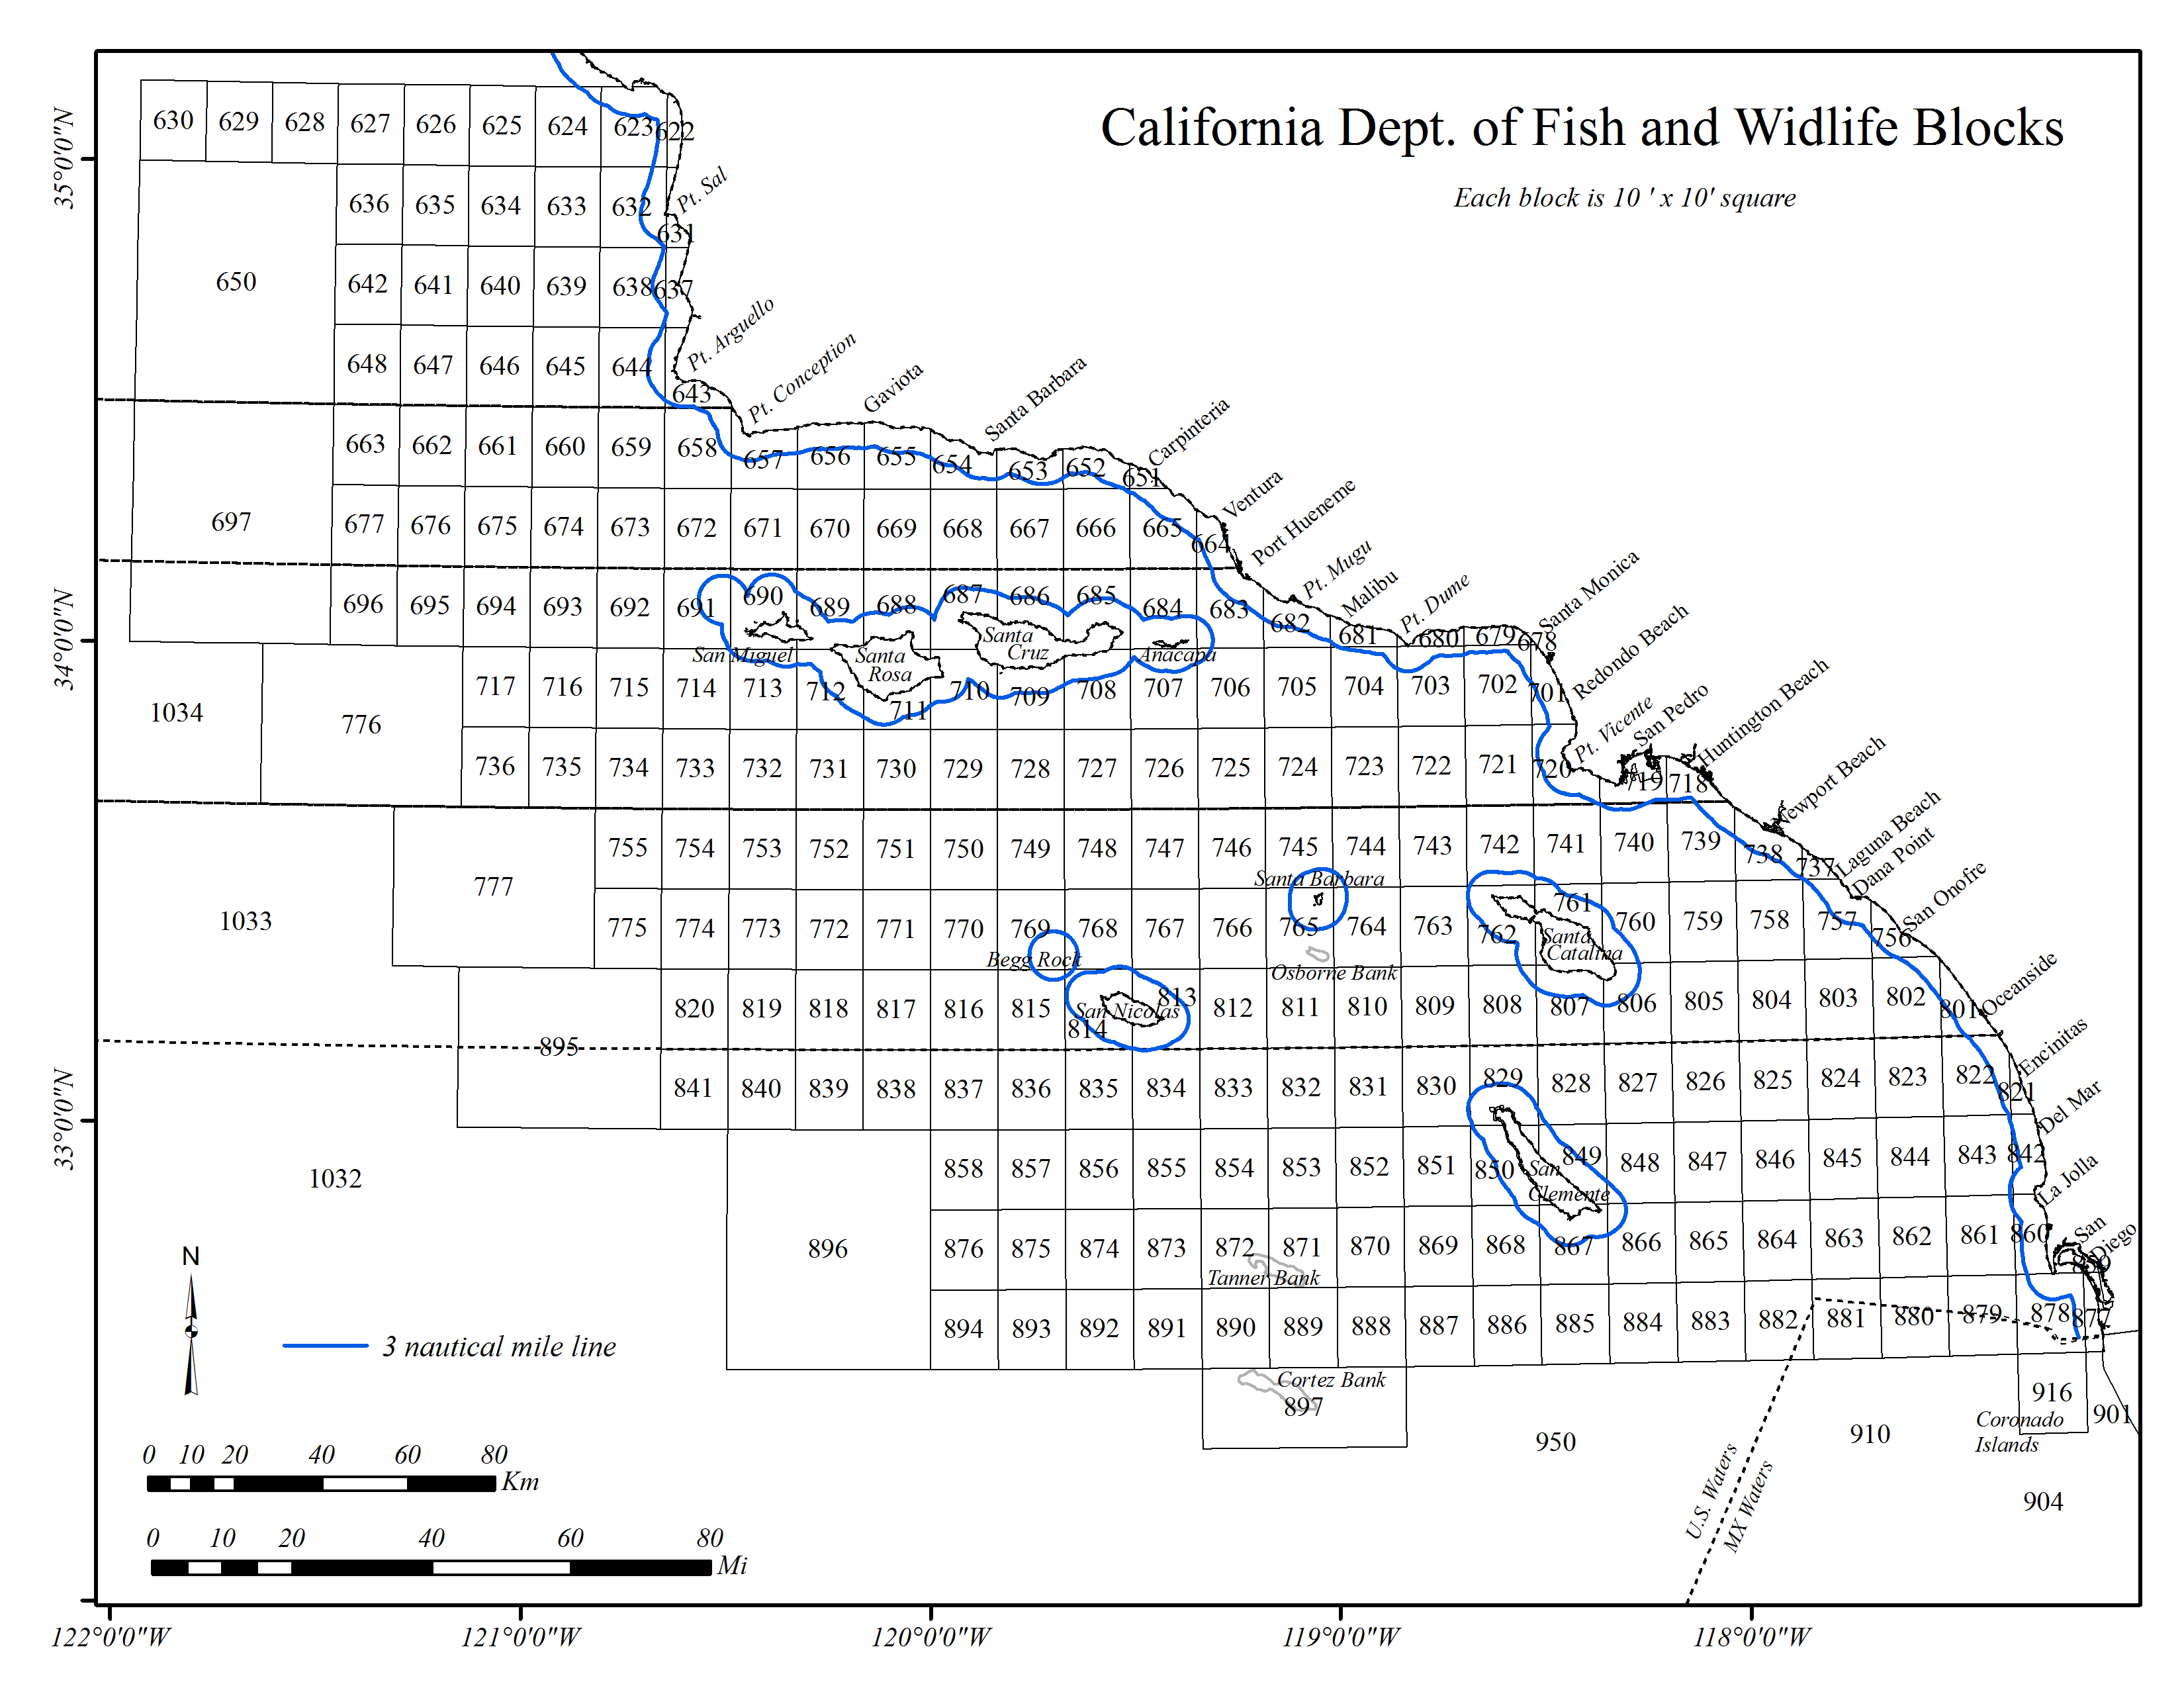
\includegraphics{Figures/boundary_map.png}
\caption{Map showing the state boundary lines for management of the
recreational fishing fleets. CRFS Districts 1-6 in California are
presented as well as the WDFW Recreational Management Areas in
Washington. Florence, OR is shown as a potential location of model
stratification. \label{fig:boundary_map}}
\end{figure}

\begin{figure}[htbp]
\centering
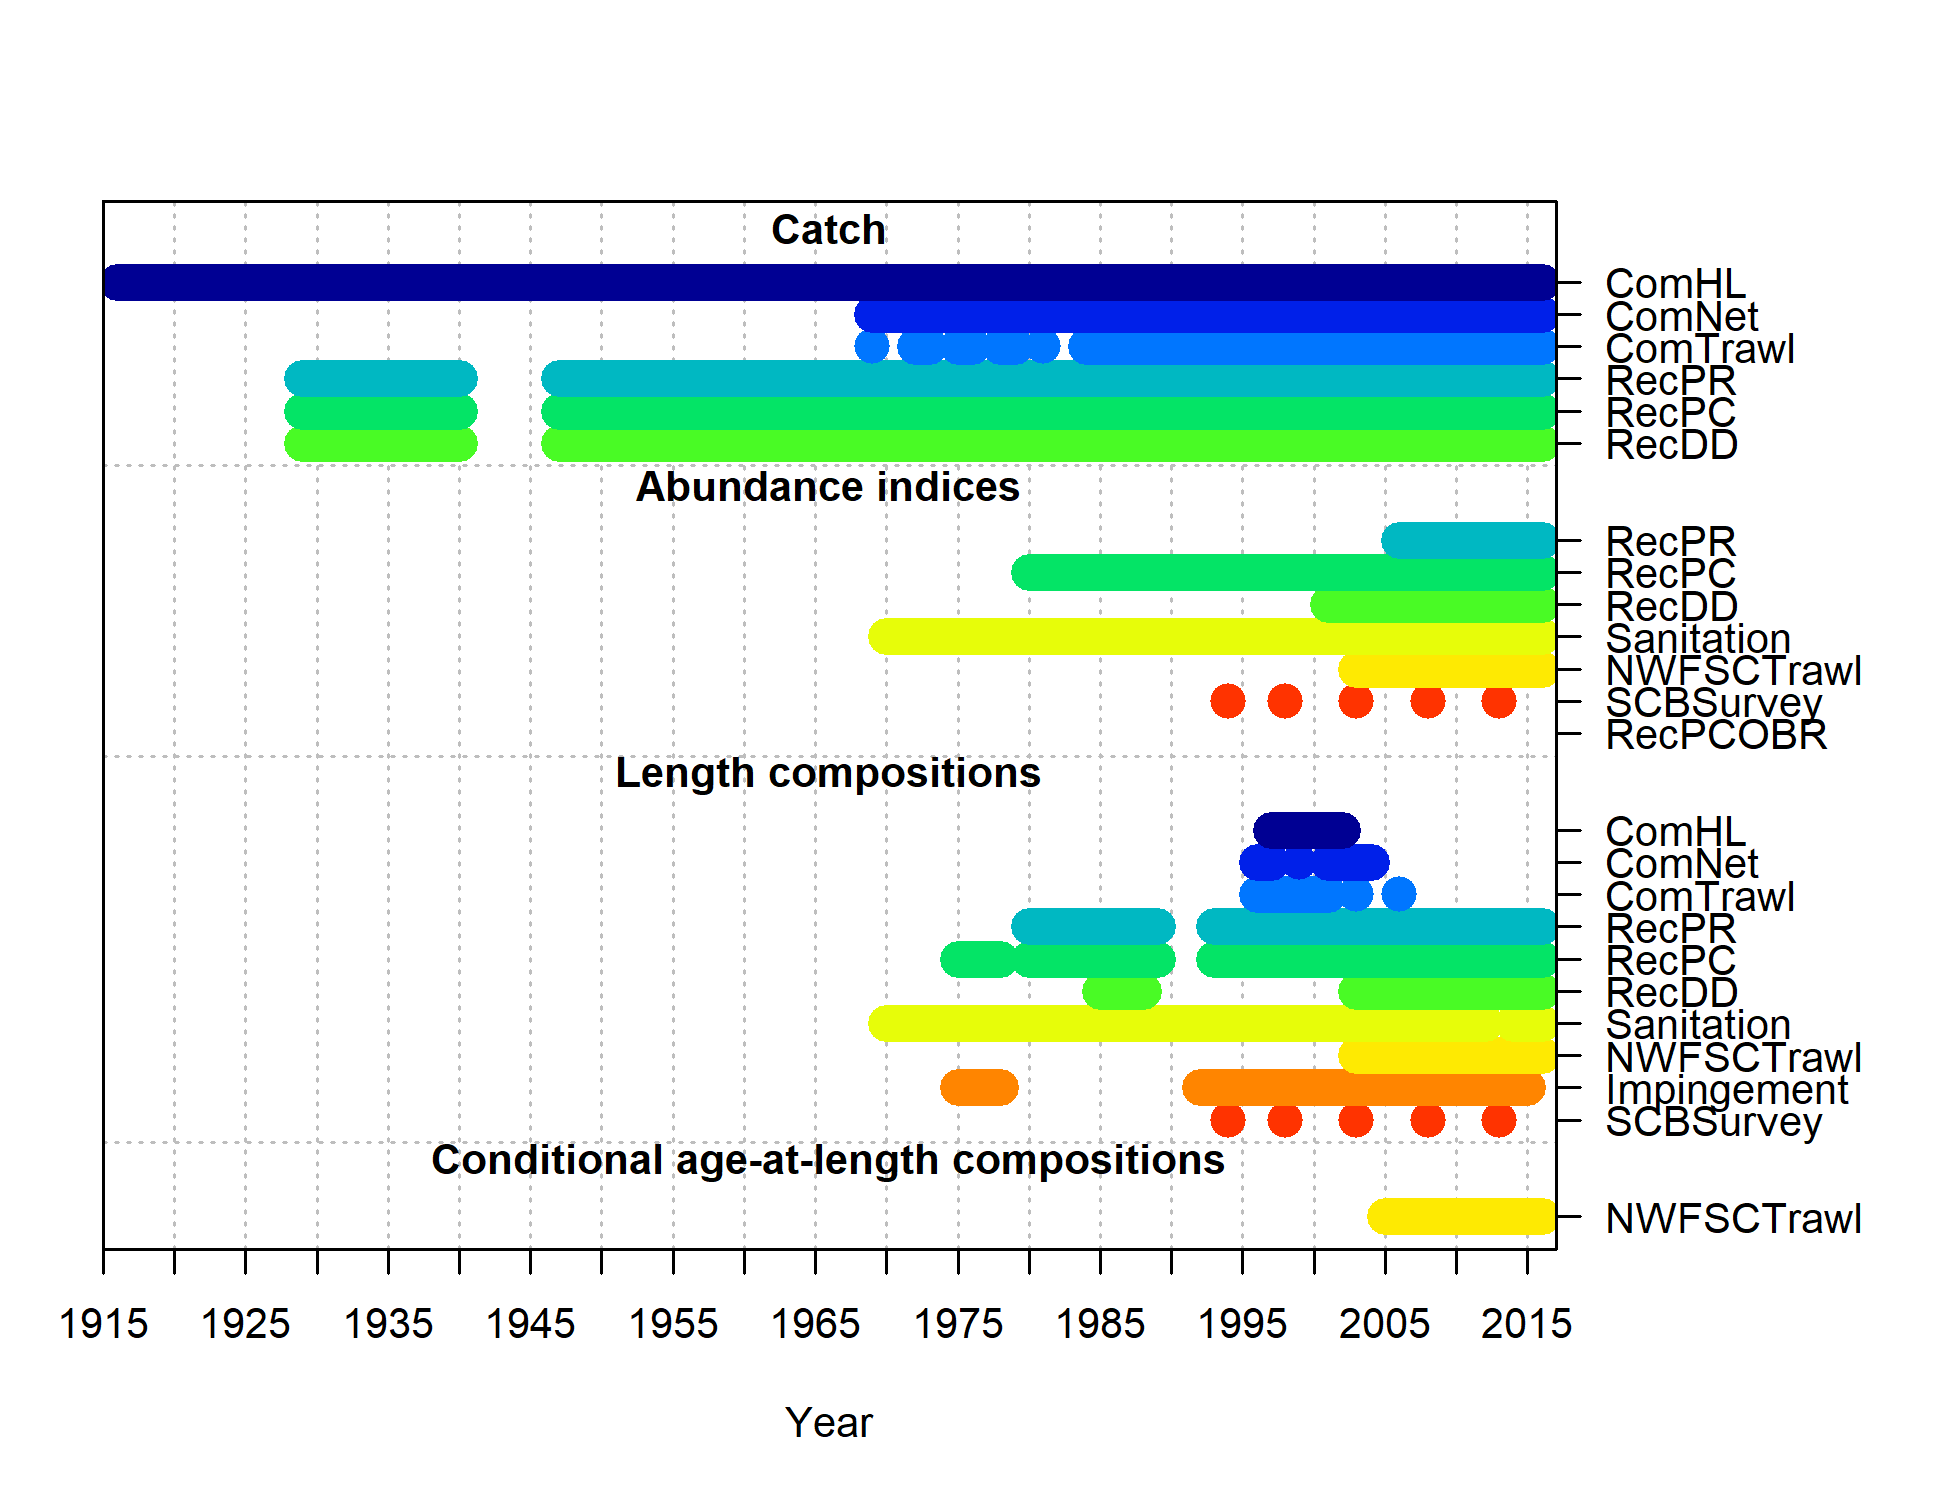
\includegraphics{r4ss/plots_mod1/data_plot.png}
\caption{Summary of data sources used in the base model.
\label{fig:data_plot}}
\end{figure}

\FloatBarrier

\FloatBarrier

\FloatBarrier

\begin{figure}[htbp]
\centering
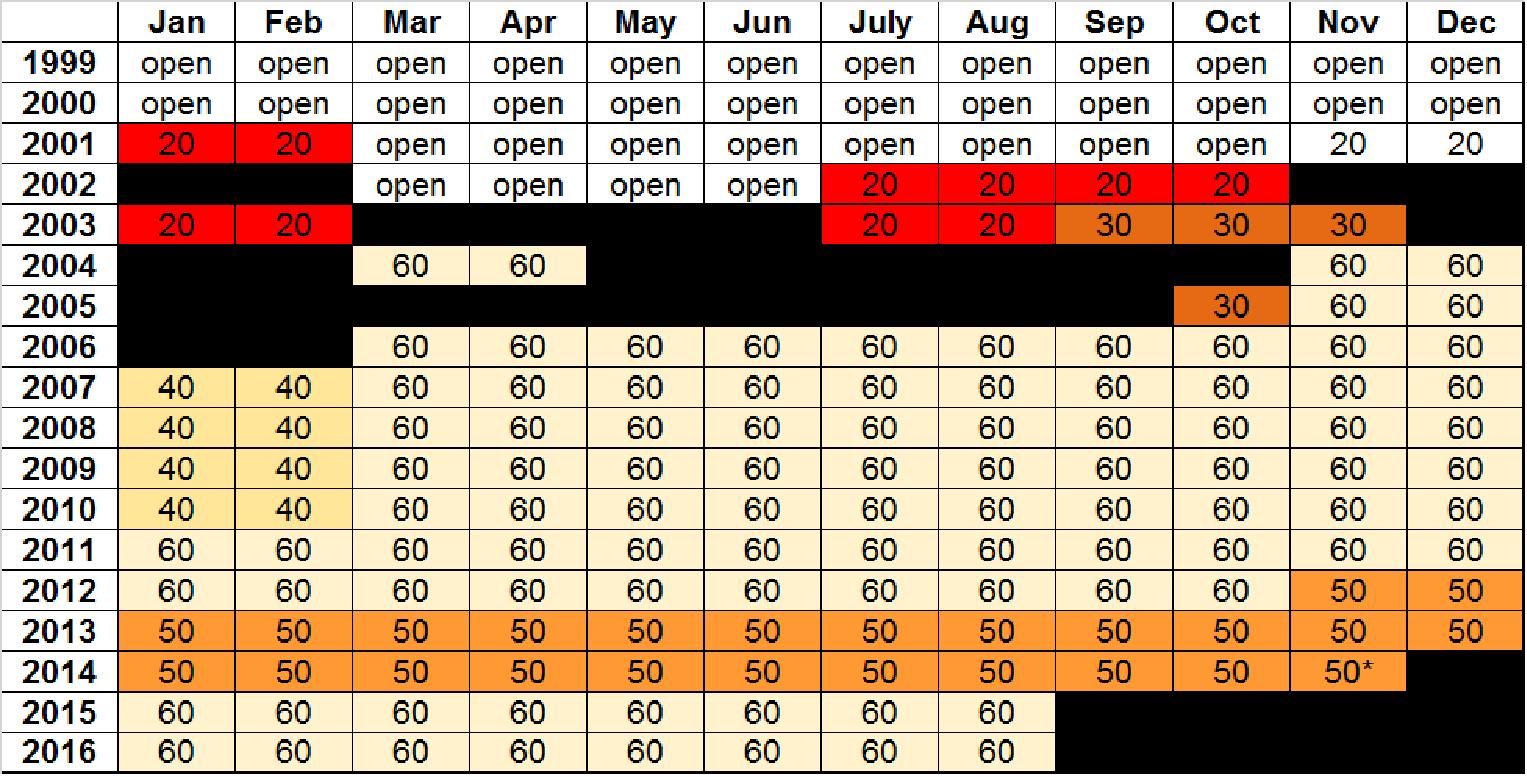
\includegraphics{Figures/Rec_regs.pdf}
\caption{A summary of the monthly recreational regulations for
California scorpionfish in southern Califoria. cells with ``open''
indicate no depth restriction, black cells indicate the fishery is
closed, and cells with a number indicate the depth restriction in
fathoms, e.g., 20 = retained catch allowed in less than 20 fathoms.
*Fishery closed on November 15, 2014. \label{fig:recregs}}
\end{figure}

\begin{figure}[htbp]
\centering
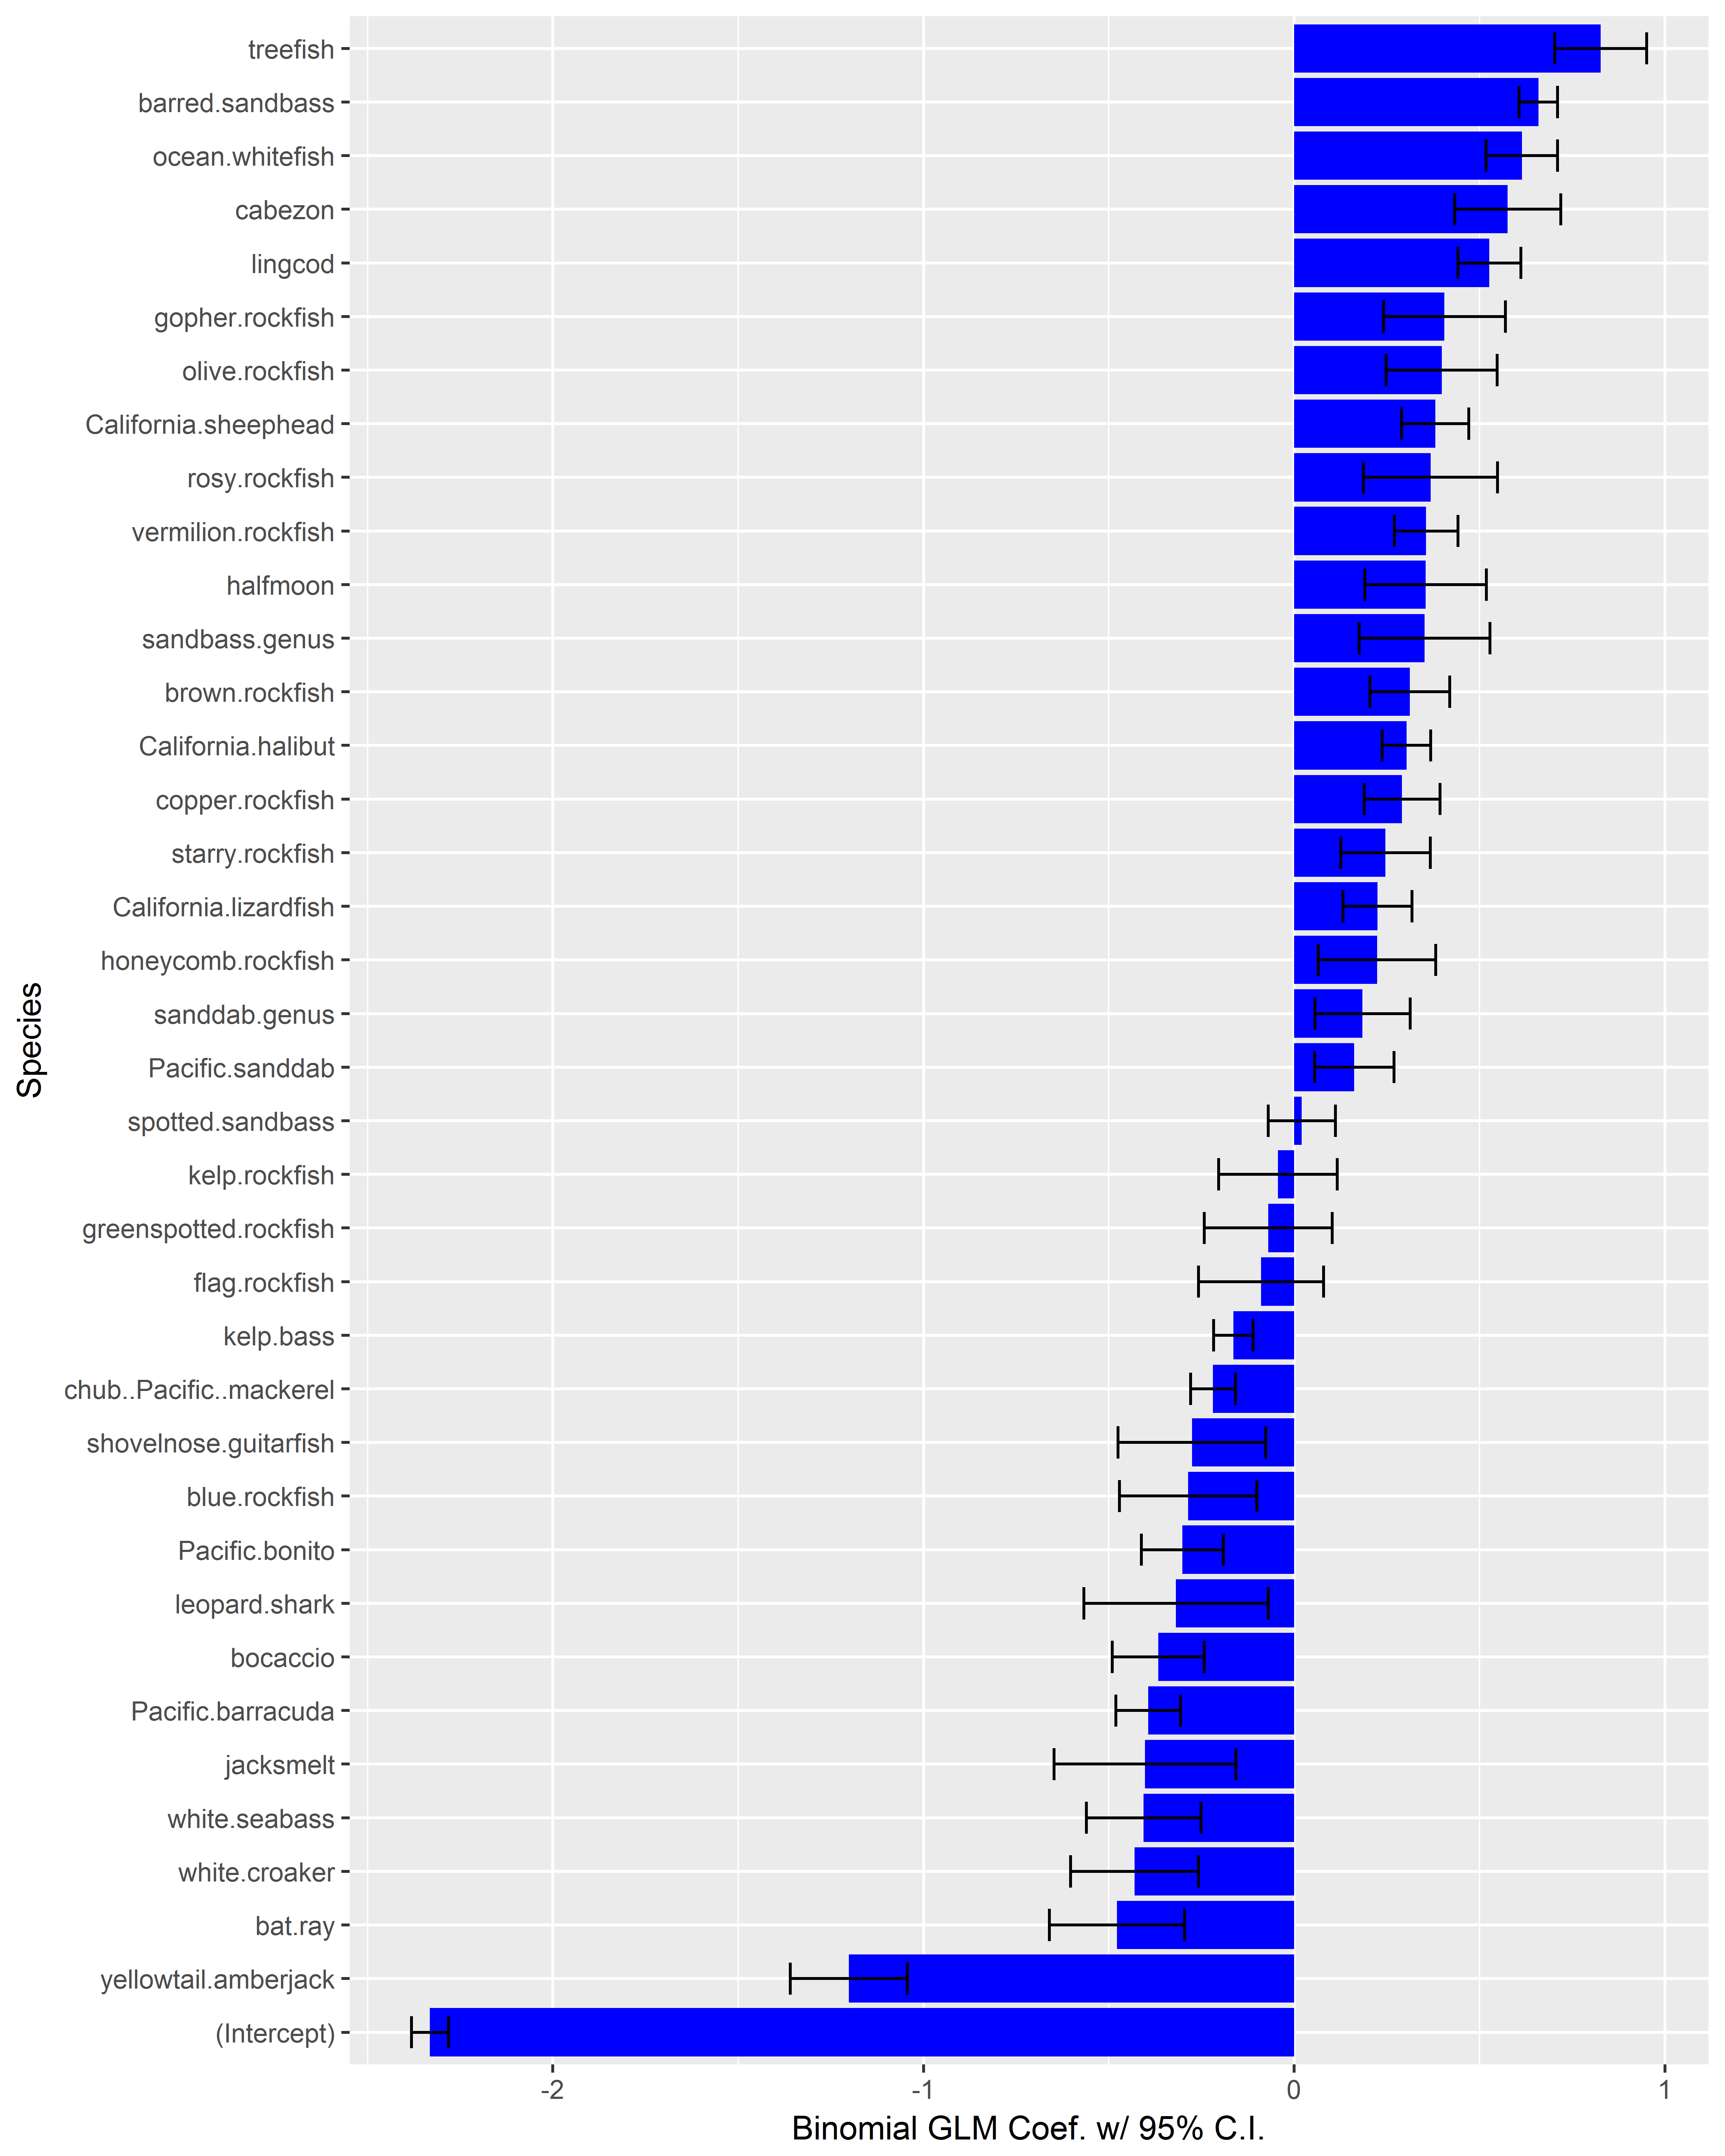
\includegraphics{Figures/Fleet4_RecPR_SMcoef.png}
\caption{Species coefficients from the binomial GLM for presence/absence
of California scorpionfish in the Marine Recreational Fisheries
Statistics Survey (MRFSS) private mode dockside survey data set.
Horizontal bars are 95\% confidence intervals.
\label{fig:Fleet4_RecPR_dockside_SM}}
\end{figure}

\begin{figure}[htbp]
\centering
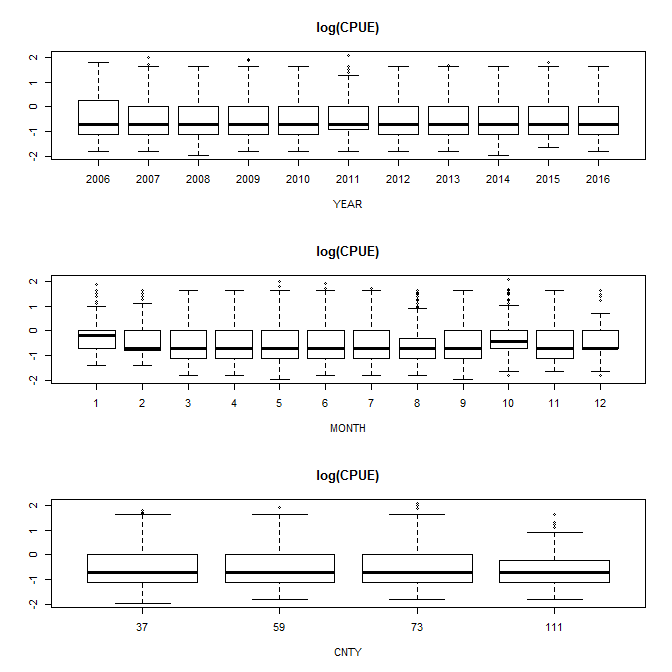
\includegraphics{Figures/Fleet4_RecPR_dockside_lograwCPUE.png}
\caption{Boxplots of the raw log CPUE by year for each of the three
factors considered in the deltaGLM model, county, month and year.
\label{fig:Fleet4_RecPR_dockside_lograwCPUE}}
\end{figure}

\begin{figure}[htbp]
\centering
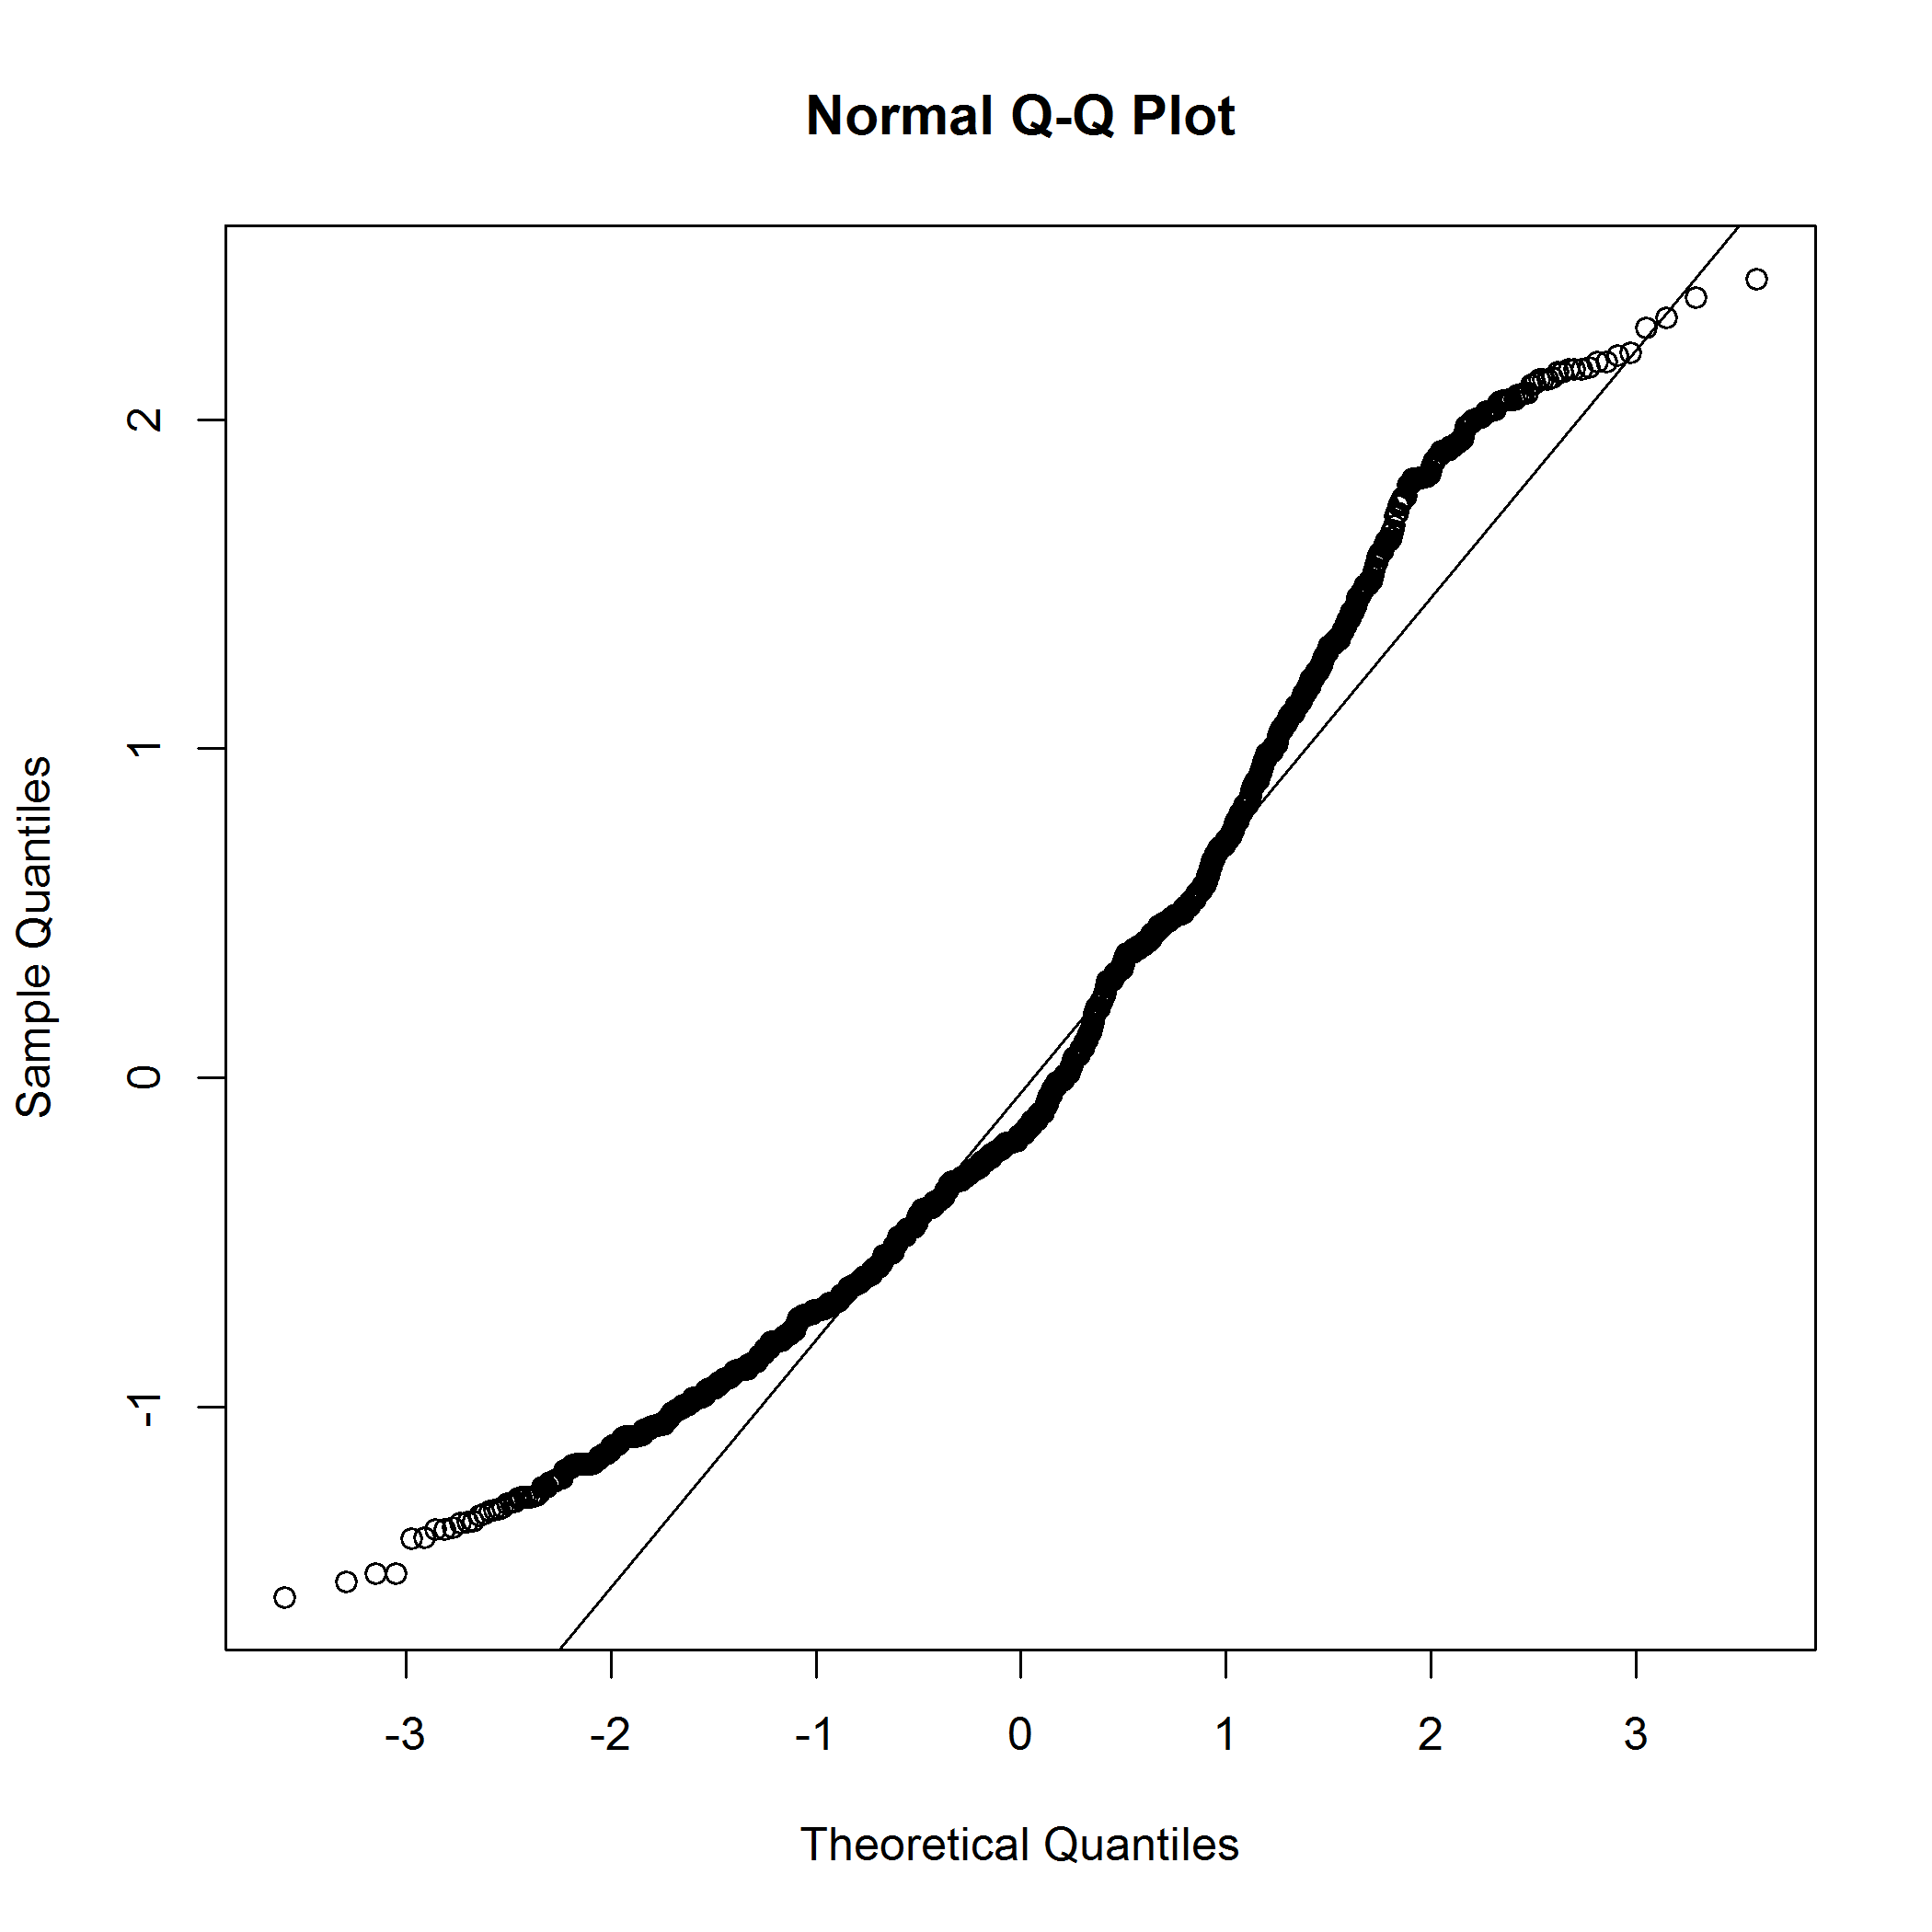
\includegraphics{Figures/Fleet4_RecPR_dockside_QQ.png}
\caption{Q-Q plot used to evaluate the fit of the lognmoral (positive
encounters) of California scorpionfish from the Marine Recreational
Fisheries Statistics Survey (MRFSS) private mode dockside survey data
set. \label{fig:Fleet4_RecPR_dockside_QQ}}
\end{figure}

\begin{figure}[htbp]
\centering
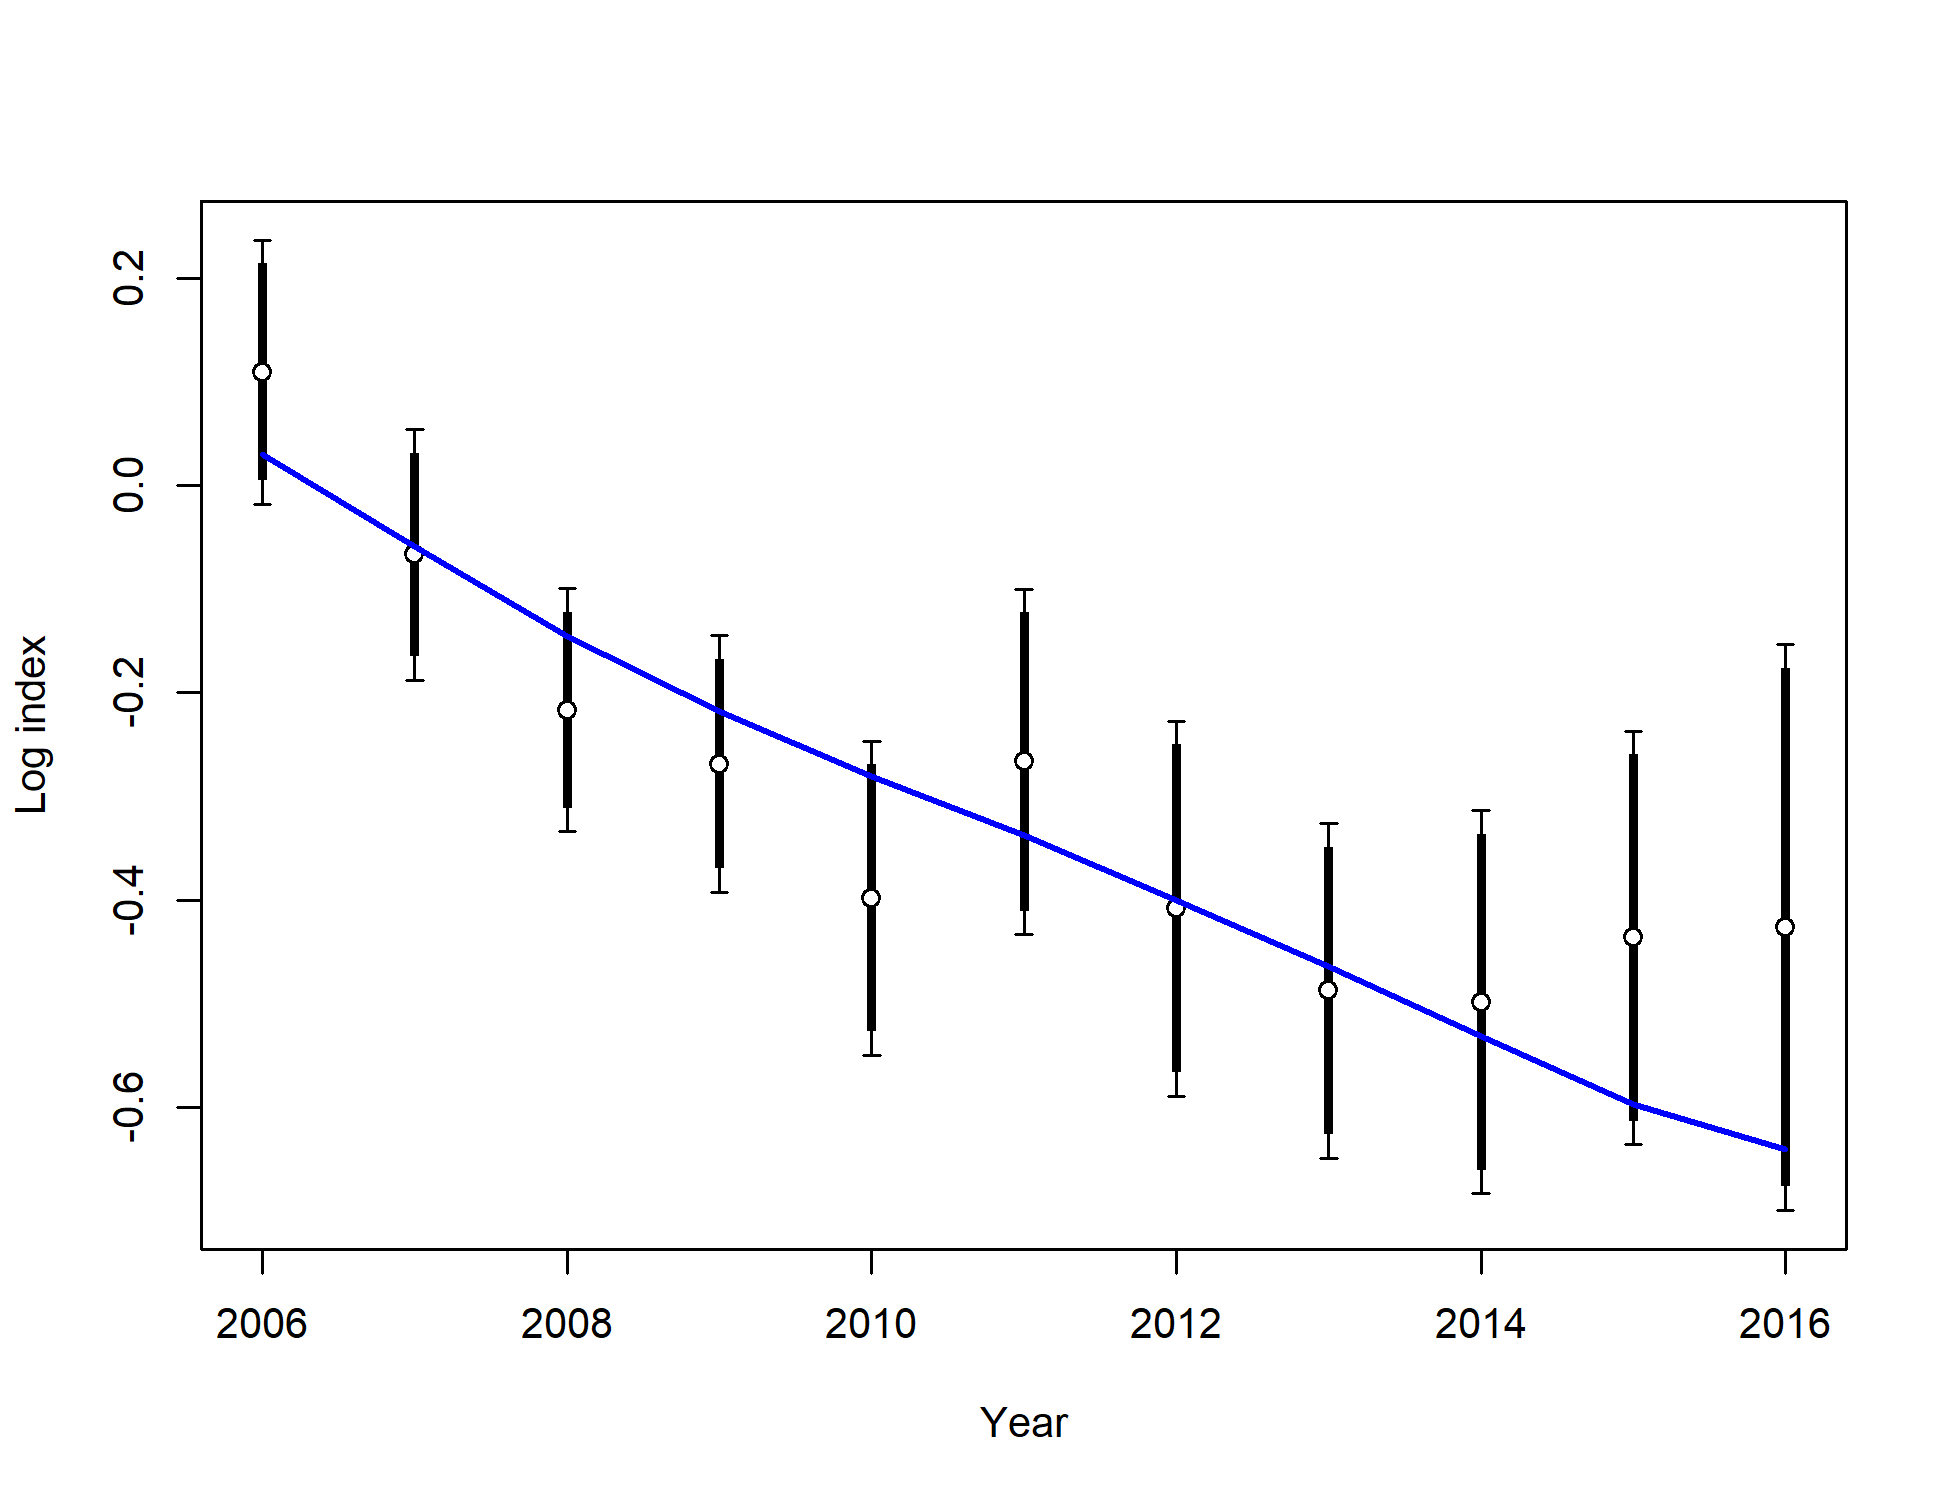
\includegraphics{r4ss/plots_mod1/index5_logcpuefit_RecPR.png}
\caption{Fit to log index data on log scale for the recreational CPFV
logbook retained catches. Lines indicate 95\% uncertainty interval
around index values. Thicker lines indicate input uncertainty before
addition of estimated additional uncertainty parameter.
\label{fig:index5_logcpuefit_RecPR}}
\end{figure}

\FloatBarrier

\begin{figure}[htbp]
\centering
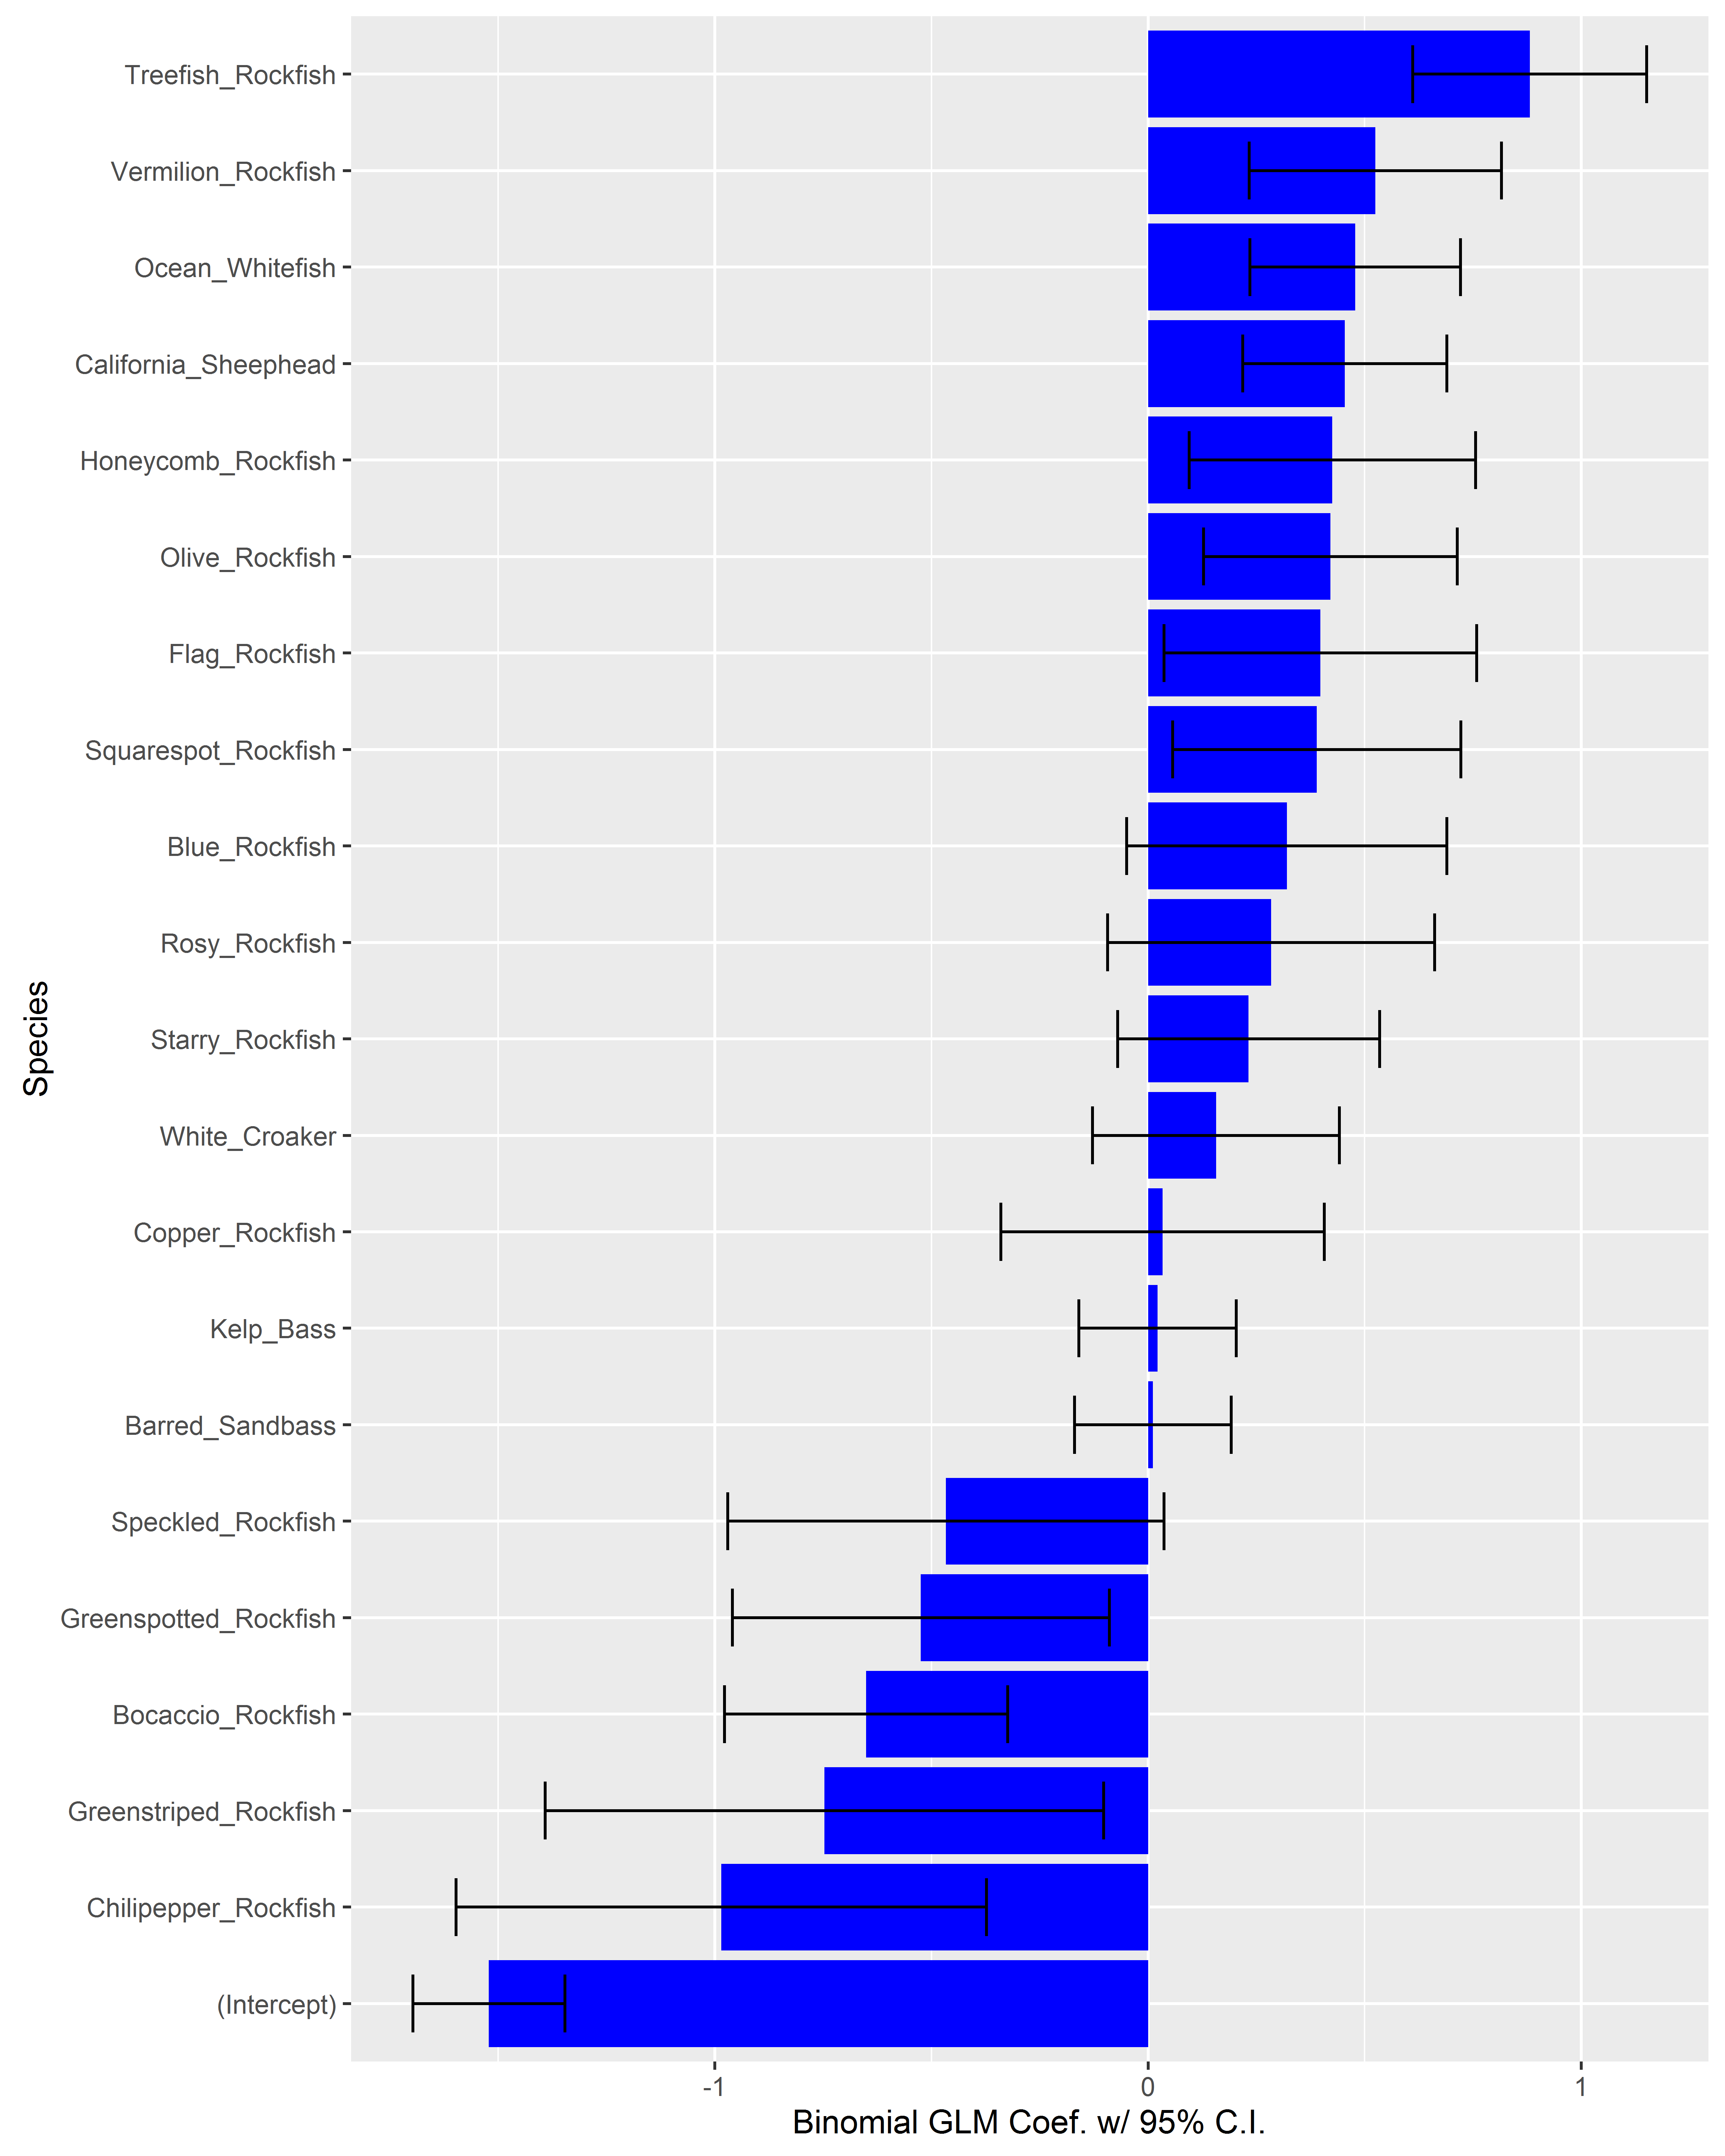
\includegraphics{Figures/Fleet5_RecPC_dockside_SM.png}
\caption{Species coefficients from the binomial GLM for presence/absence
of California scorpionfish in the Marine Recreational Fisheries
Statistics Survey (MRFSS) party/charter mode dockside survey data set.
Horizontal bars are 95\% confidence intervals.
\label{fig:Fleet5_RecPC_docksideSM}}
\end{figure}

\begin{figure}[htbp]
\centering
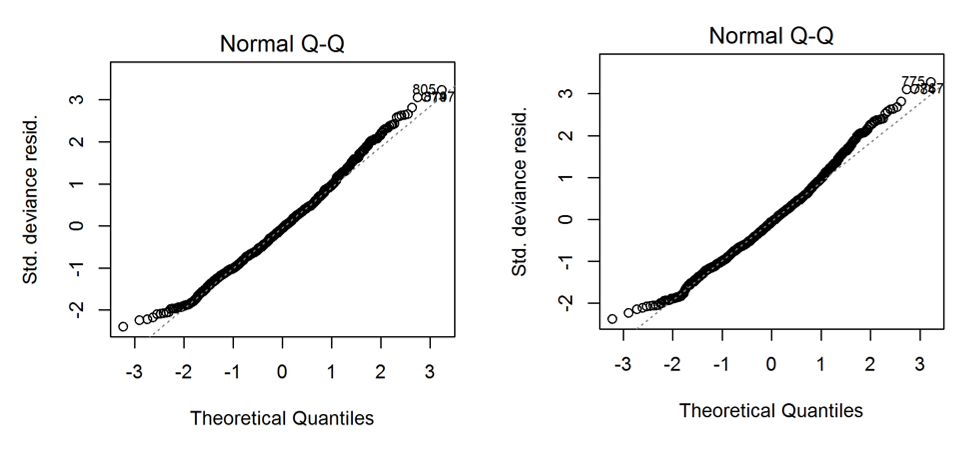
\includegraphics{Figures/Fleet5_RecPC_dockside_QQ.png}
\caption{Q-Q plot used to validate the goodness of fit of the lognormal
portion (posirive catch) of the Marine Recreational Fisheries Statistics
Survey (MRFSS) party/charter dockside survey, for thresholds of 0.27
(left) and 0.10 (right) from the Stephens-MacCall filter.
\label{fig:Fleet5_RecPC_docksideQQ}}
\end{figure}

\FloatBarrier

\begin{figure}[htbp]
\centering
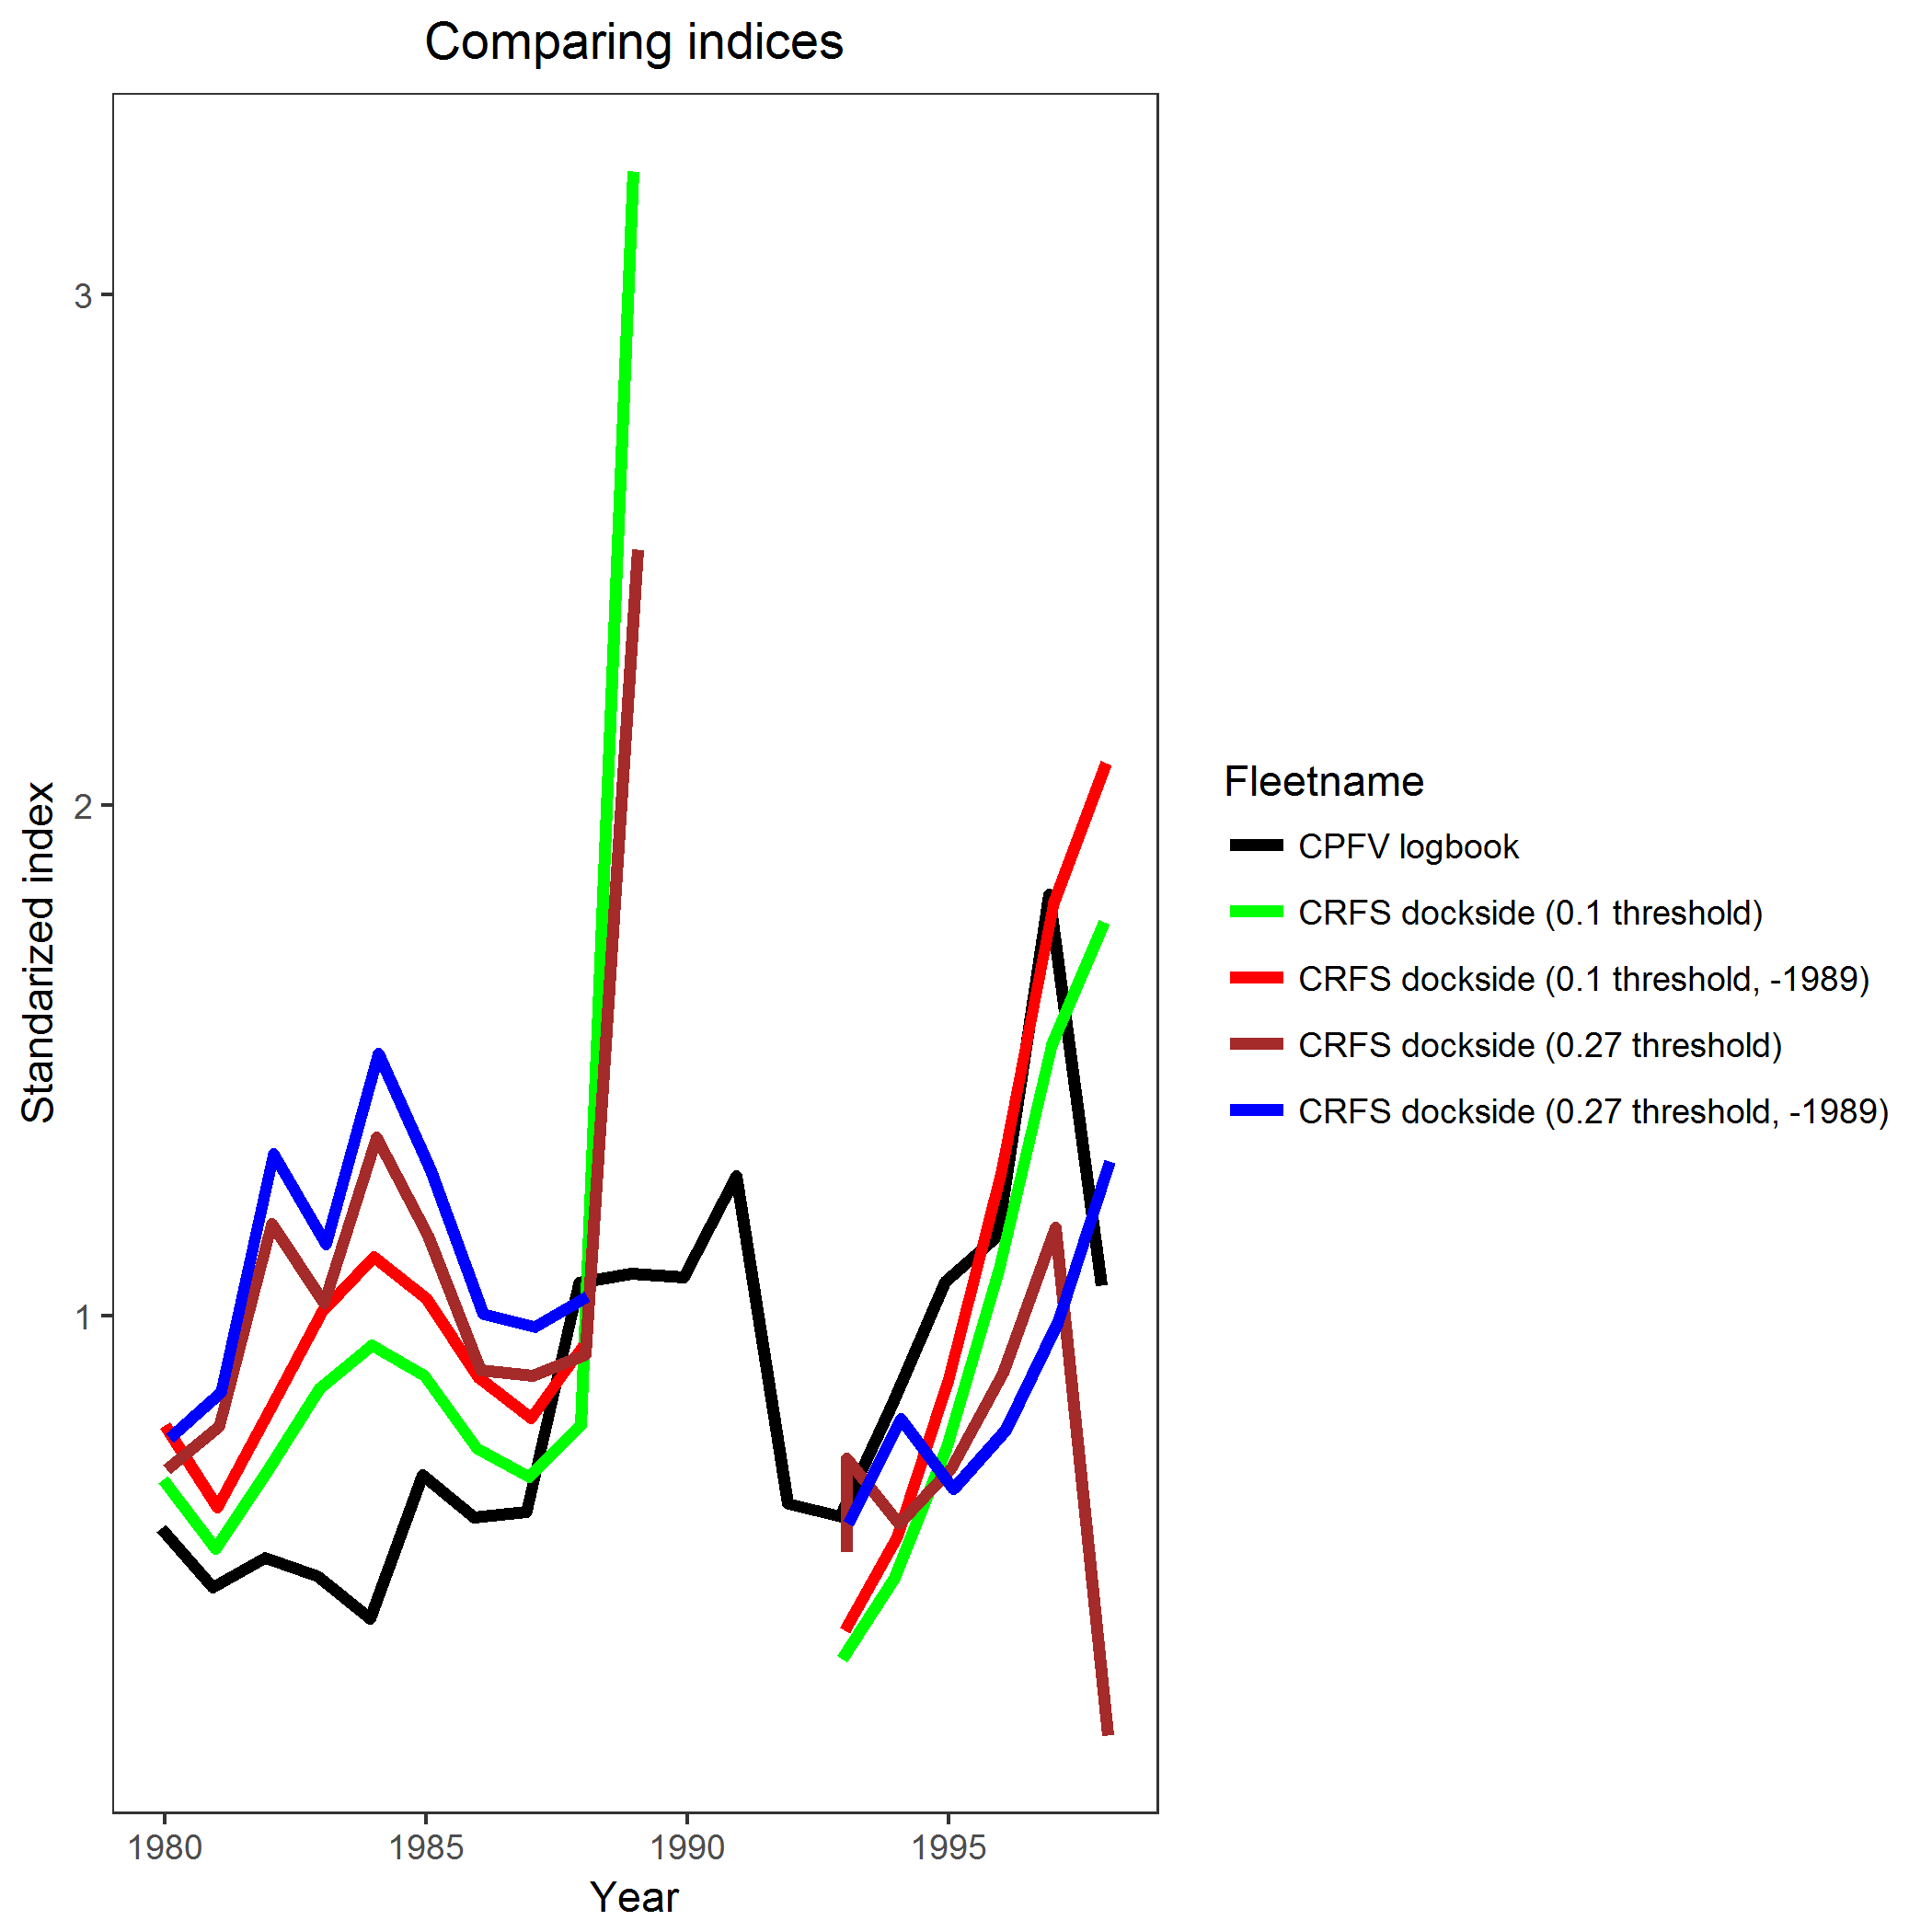
\includegraphics{Figures/Fleet5_RecPC_dockside_index_compare.png}
\caption{Comparison of standardized indices using two different
threshold levels (0.27 and 0.1) from the Stephens-MacCall filtering, and
including or excluding the year 1989.
\label{fig:Fleet5_RecPC_dockside_index_compare}}
\end{figure}

\FloatBarrier

\begin{figure}[htbp]
\centering
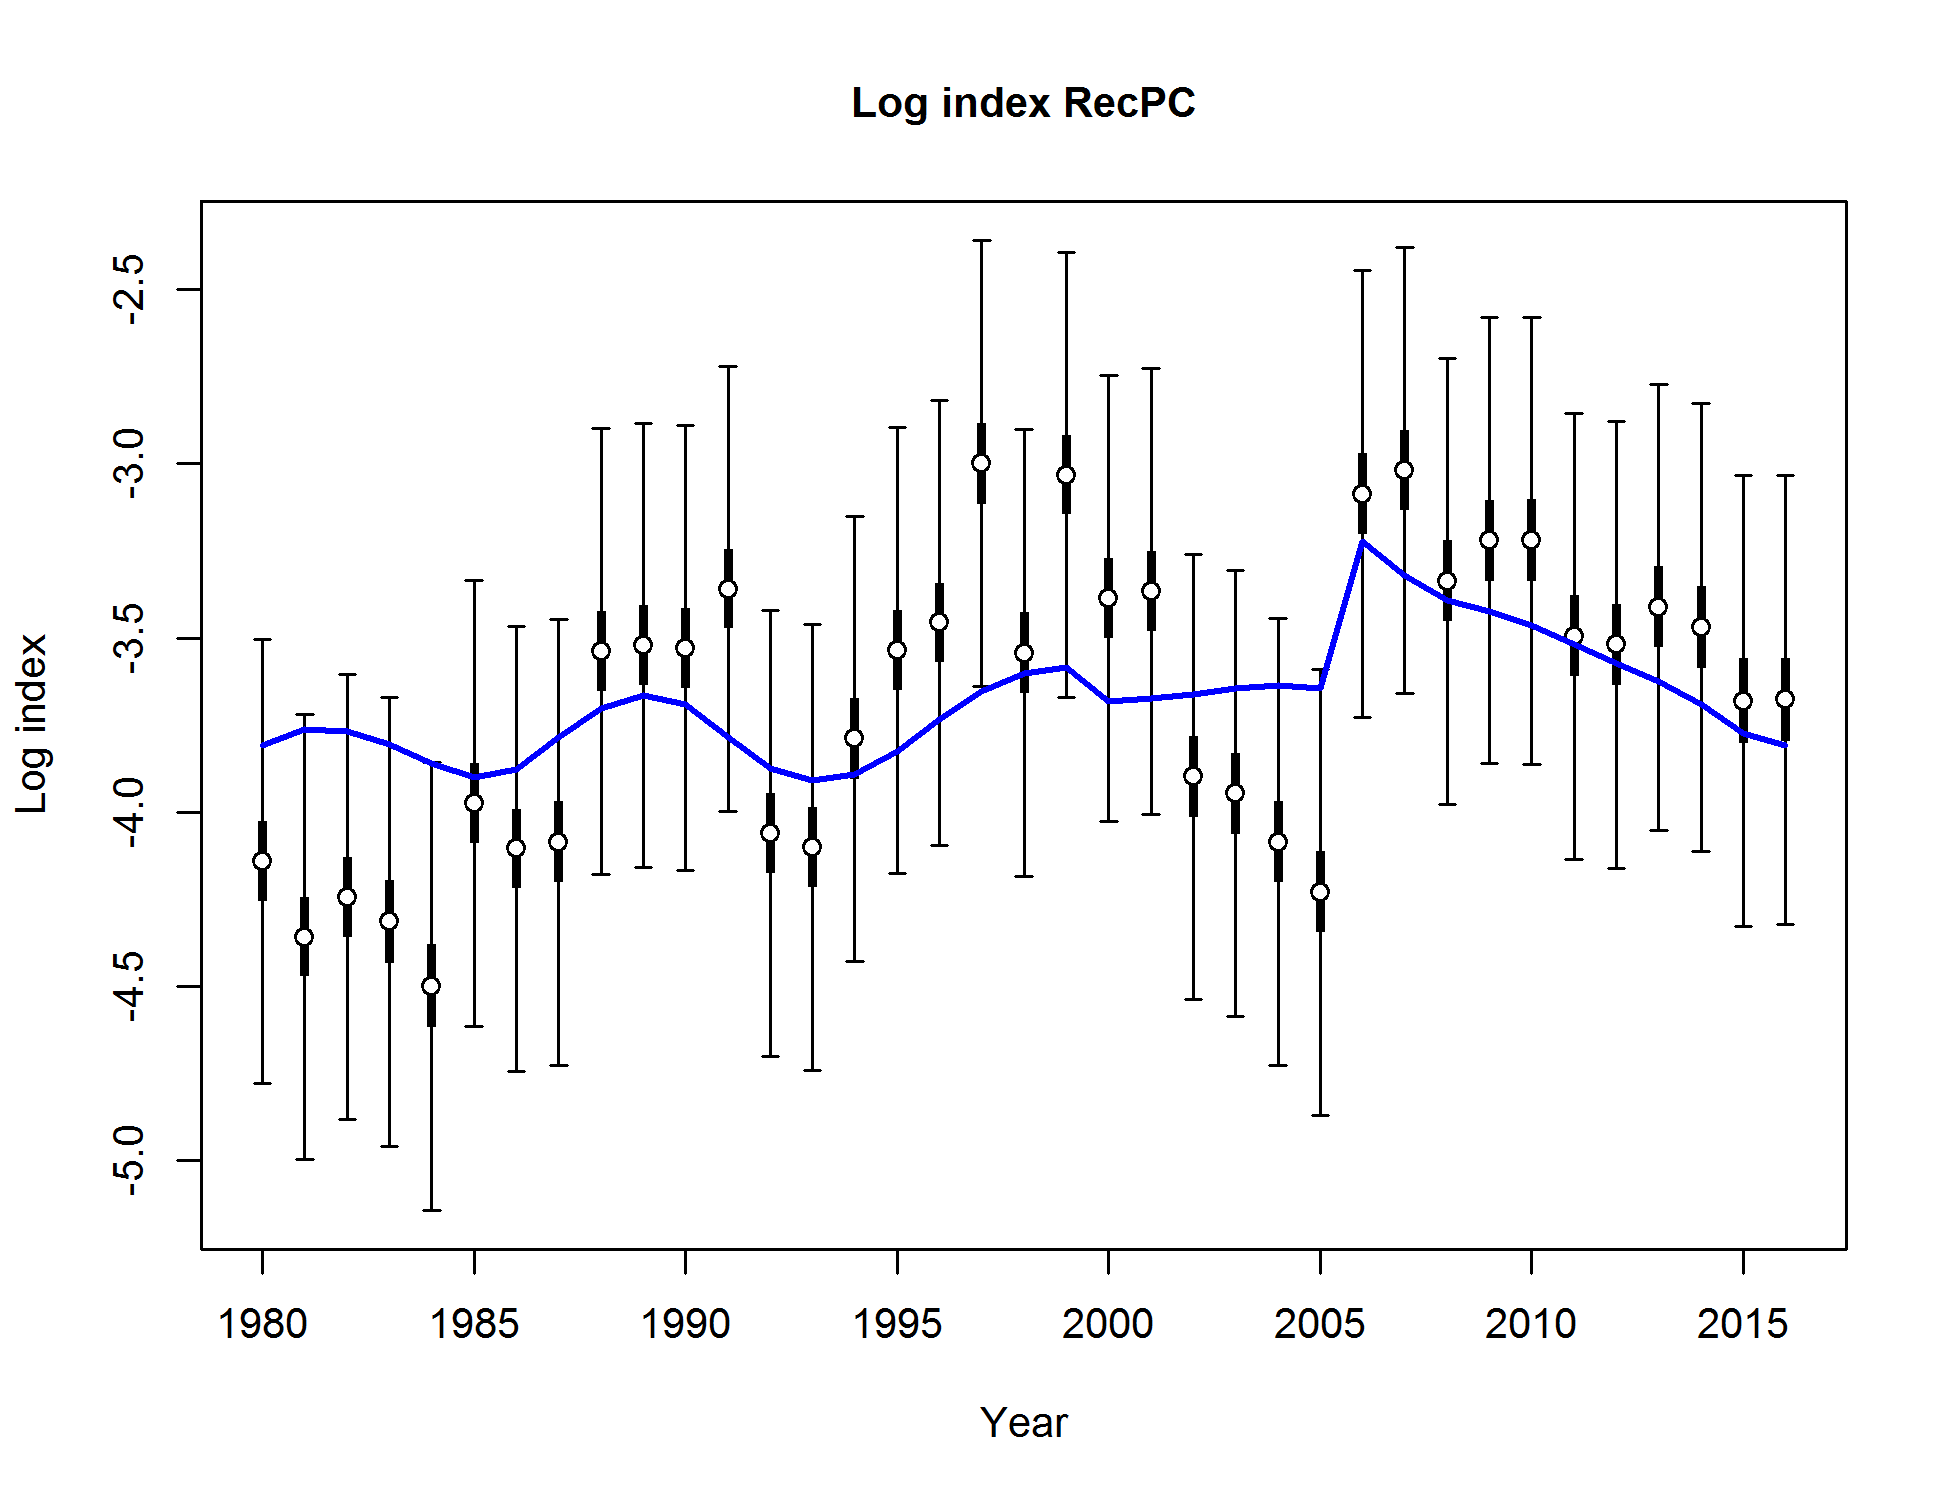
\includegraphics{r4ss/plots_mod1/index5_logcpuefit_RecPC.png}
\caption{Fit to log index data on log scale for the recreational CPFV
logbook retained catches. Lines indicate 95\% uncertainty interval
around index values. Thicker lines indicate input uncertainty before
addition of estimated additional uncertainty parameter.
\label{fig:index5_logcpuefit_RecPC}}
\end{figure}

\FloatBarrier

\begin{figure}[htbp]
\centering
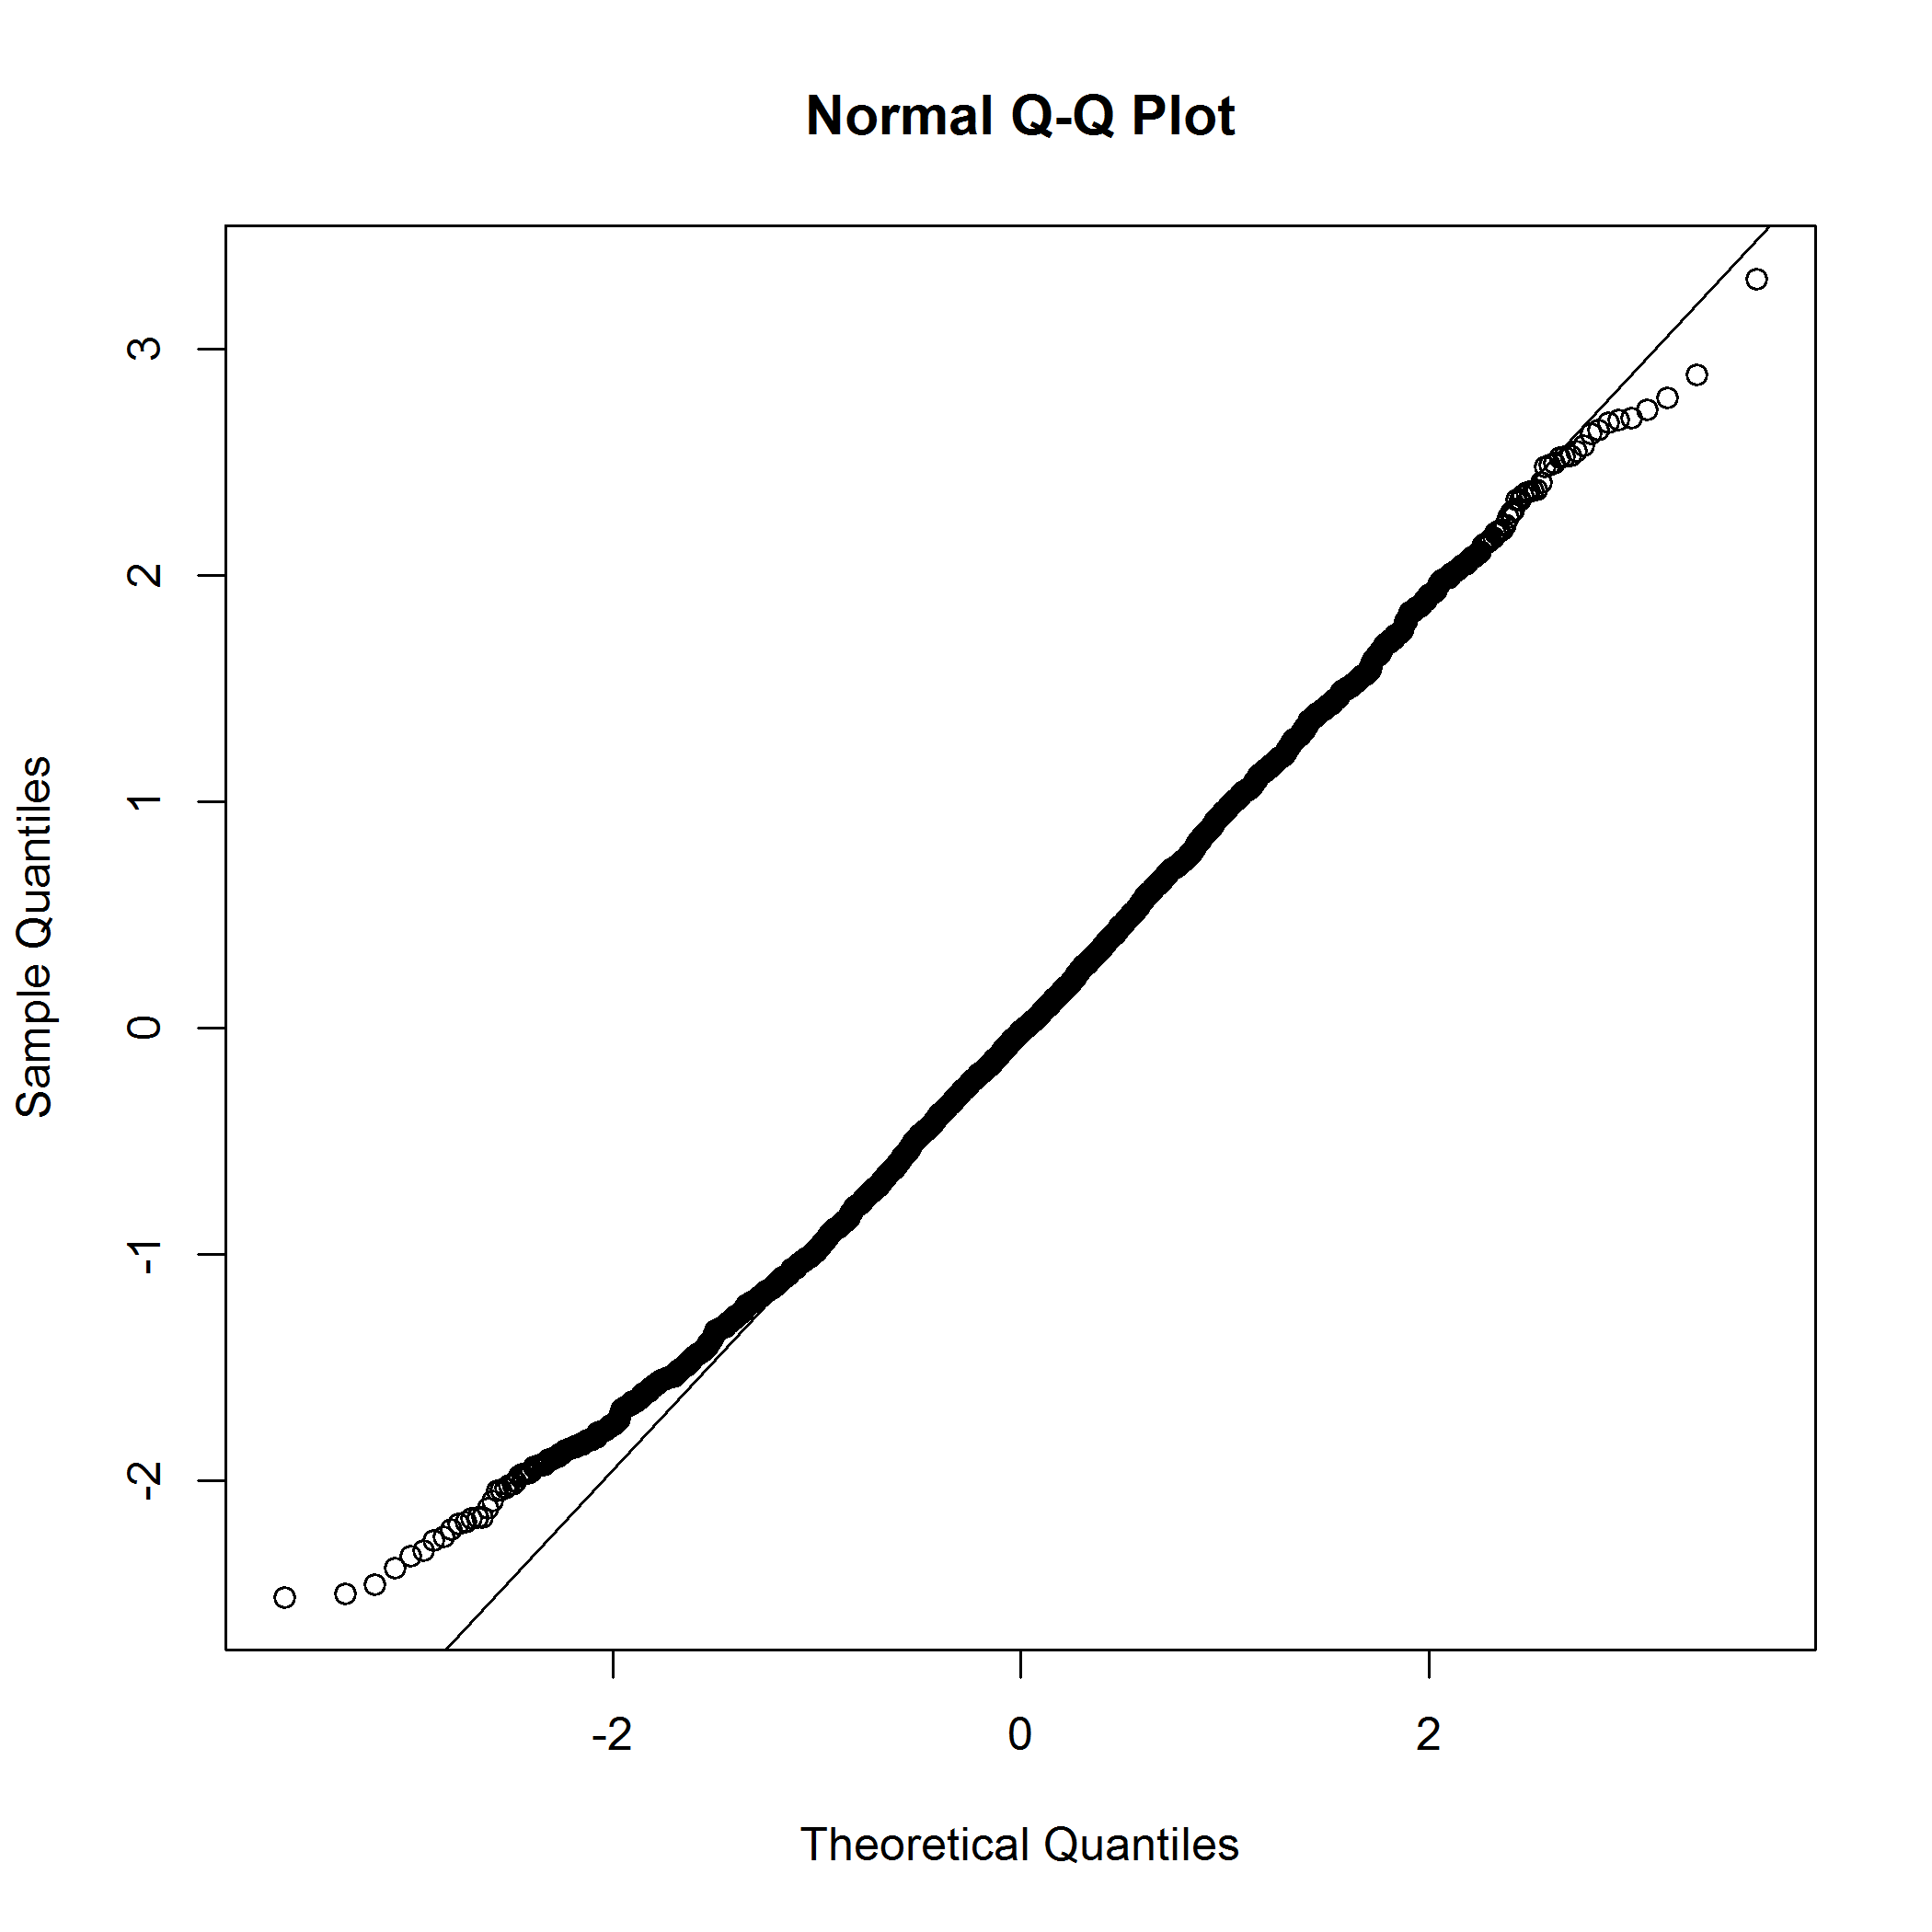
\includegraphics{Figures/Fleet6_RecDD_QQ.png}
\caption{Q-Q plot used to validate the goodness of fit of the lognormal
model for the CPFV onboard observer discarded only catch.
\label{fig:Fleet6_RecDD_QQ}}
\end{figure}

\begin{figure}[htbp]
\centering
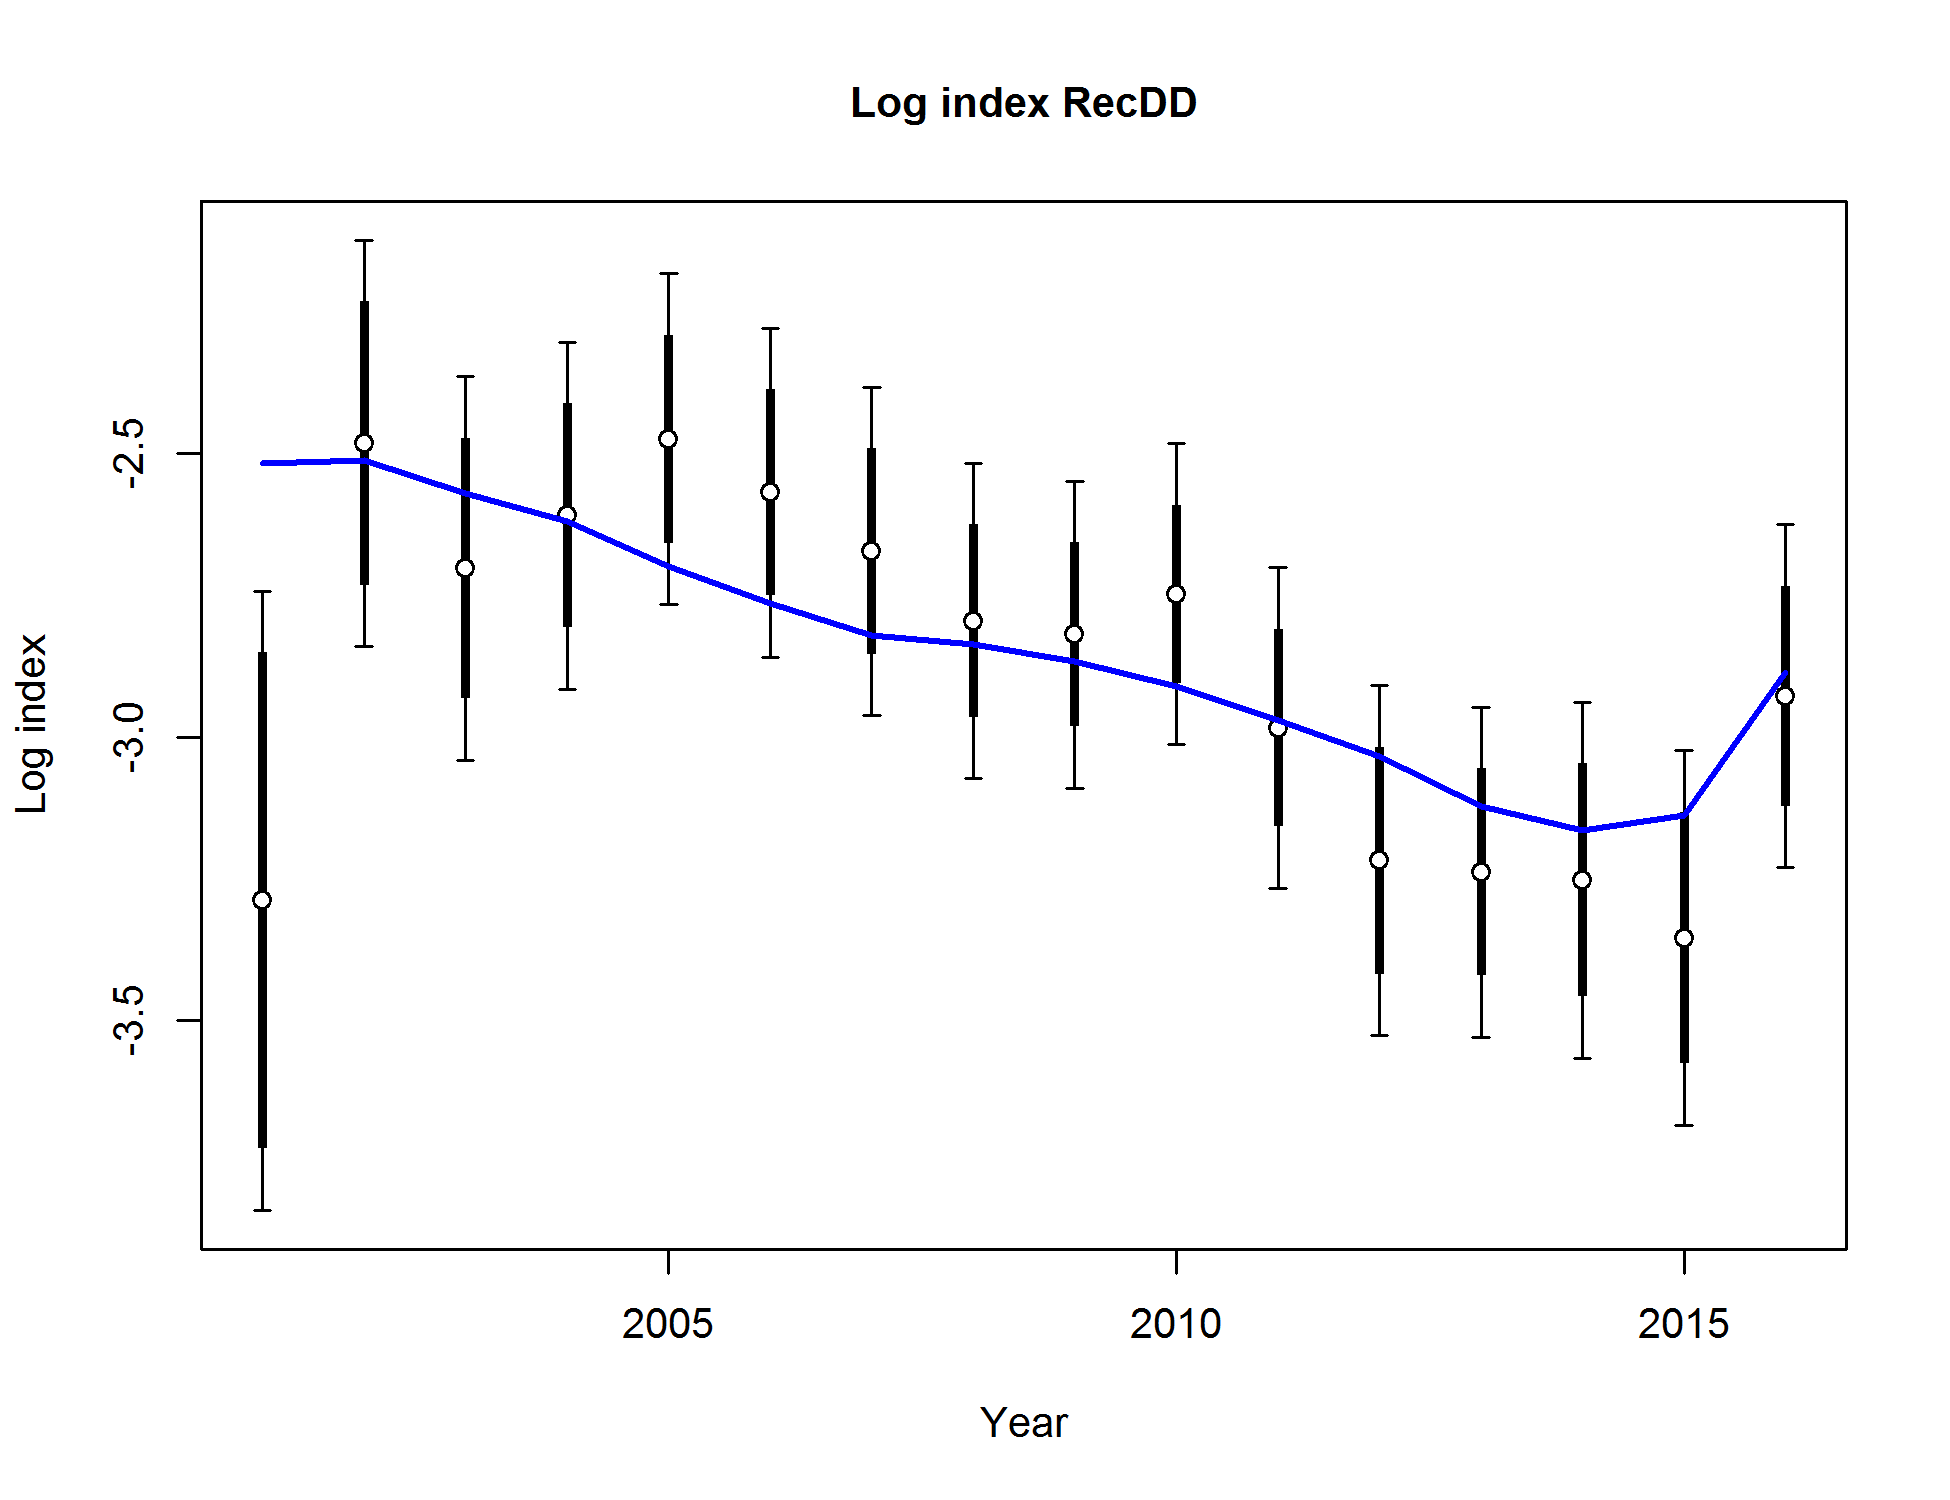
\includegraphics{r4ss/plots_mod1/index5_logcpuefit_RecDD.png}
\caption{Fit to log index data on log scale for the recreational CPFV
onboard oserver discarded catch index. Lines indicate 95\% uncertainty
interval around index values. Thicker lines indicate input uncertainty
before addition of estimated additional uncertainty parameter.
\label{fig:Fleet6_index5_logcpuefit_RecDD}}
\end{figure}

\begin{figure}[htbp]
\centering
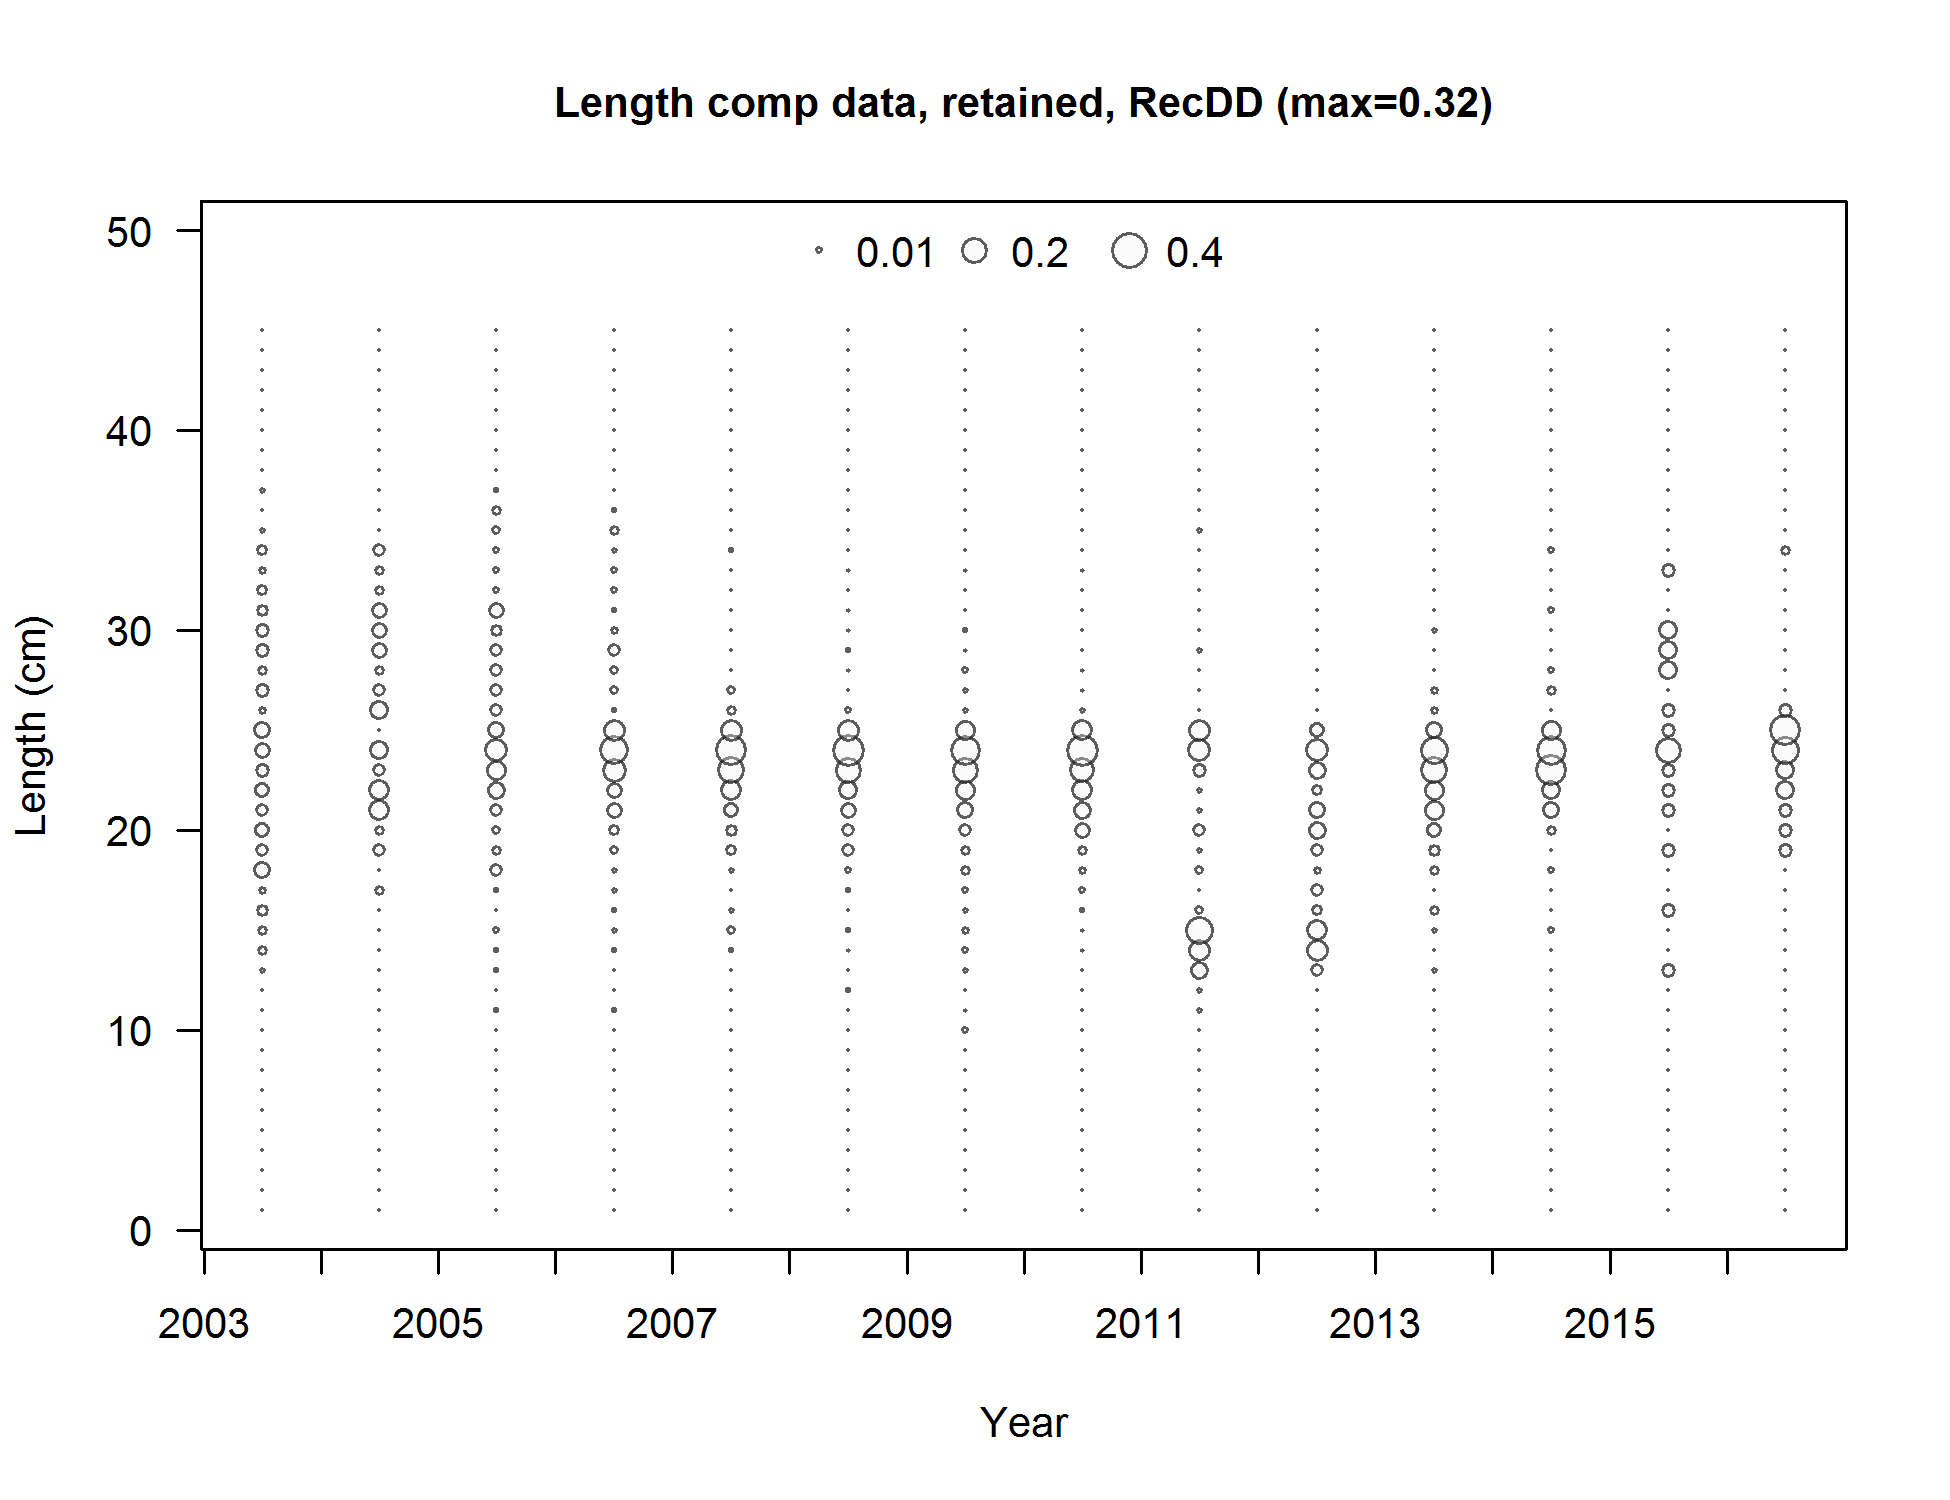
\includegraphics{r4ss/plots_mod1/comp_lendat_bubflt6mkt2.png}
\caption{Length frequency distributions from the sanitation disricts
trawl surveys. \label{fig:Fleet6_comp_lendat_bubflt6mkt2}}
\end{figure}

\begin{figure}[htbp]
\centering
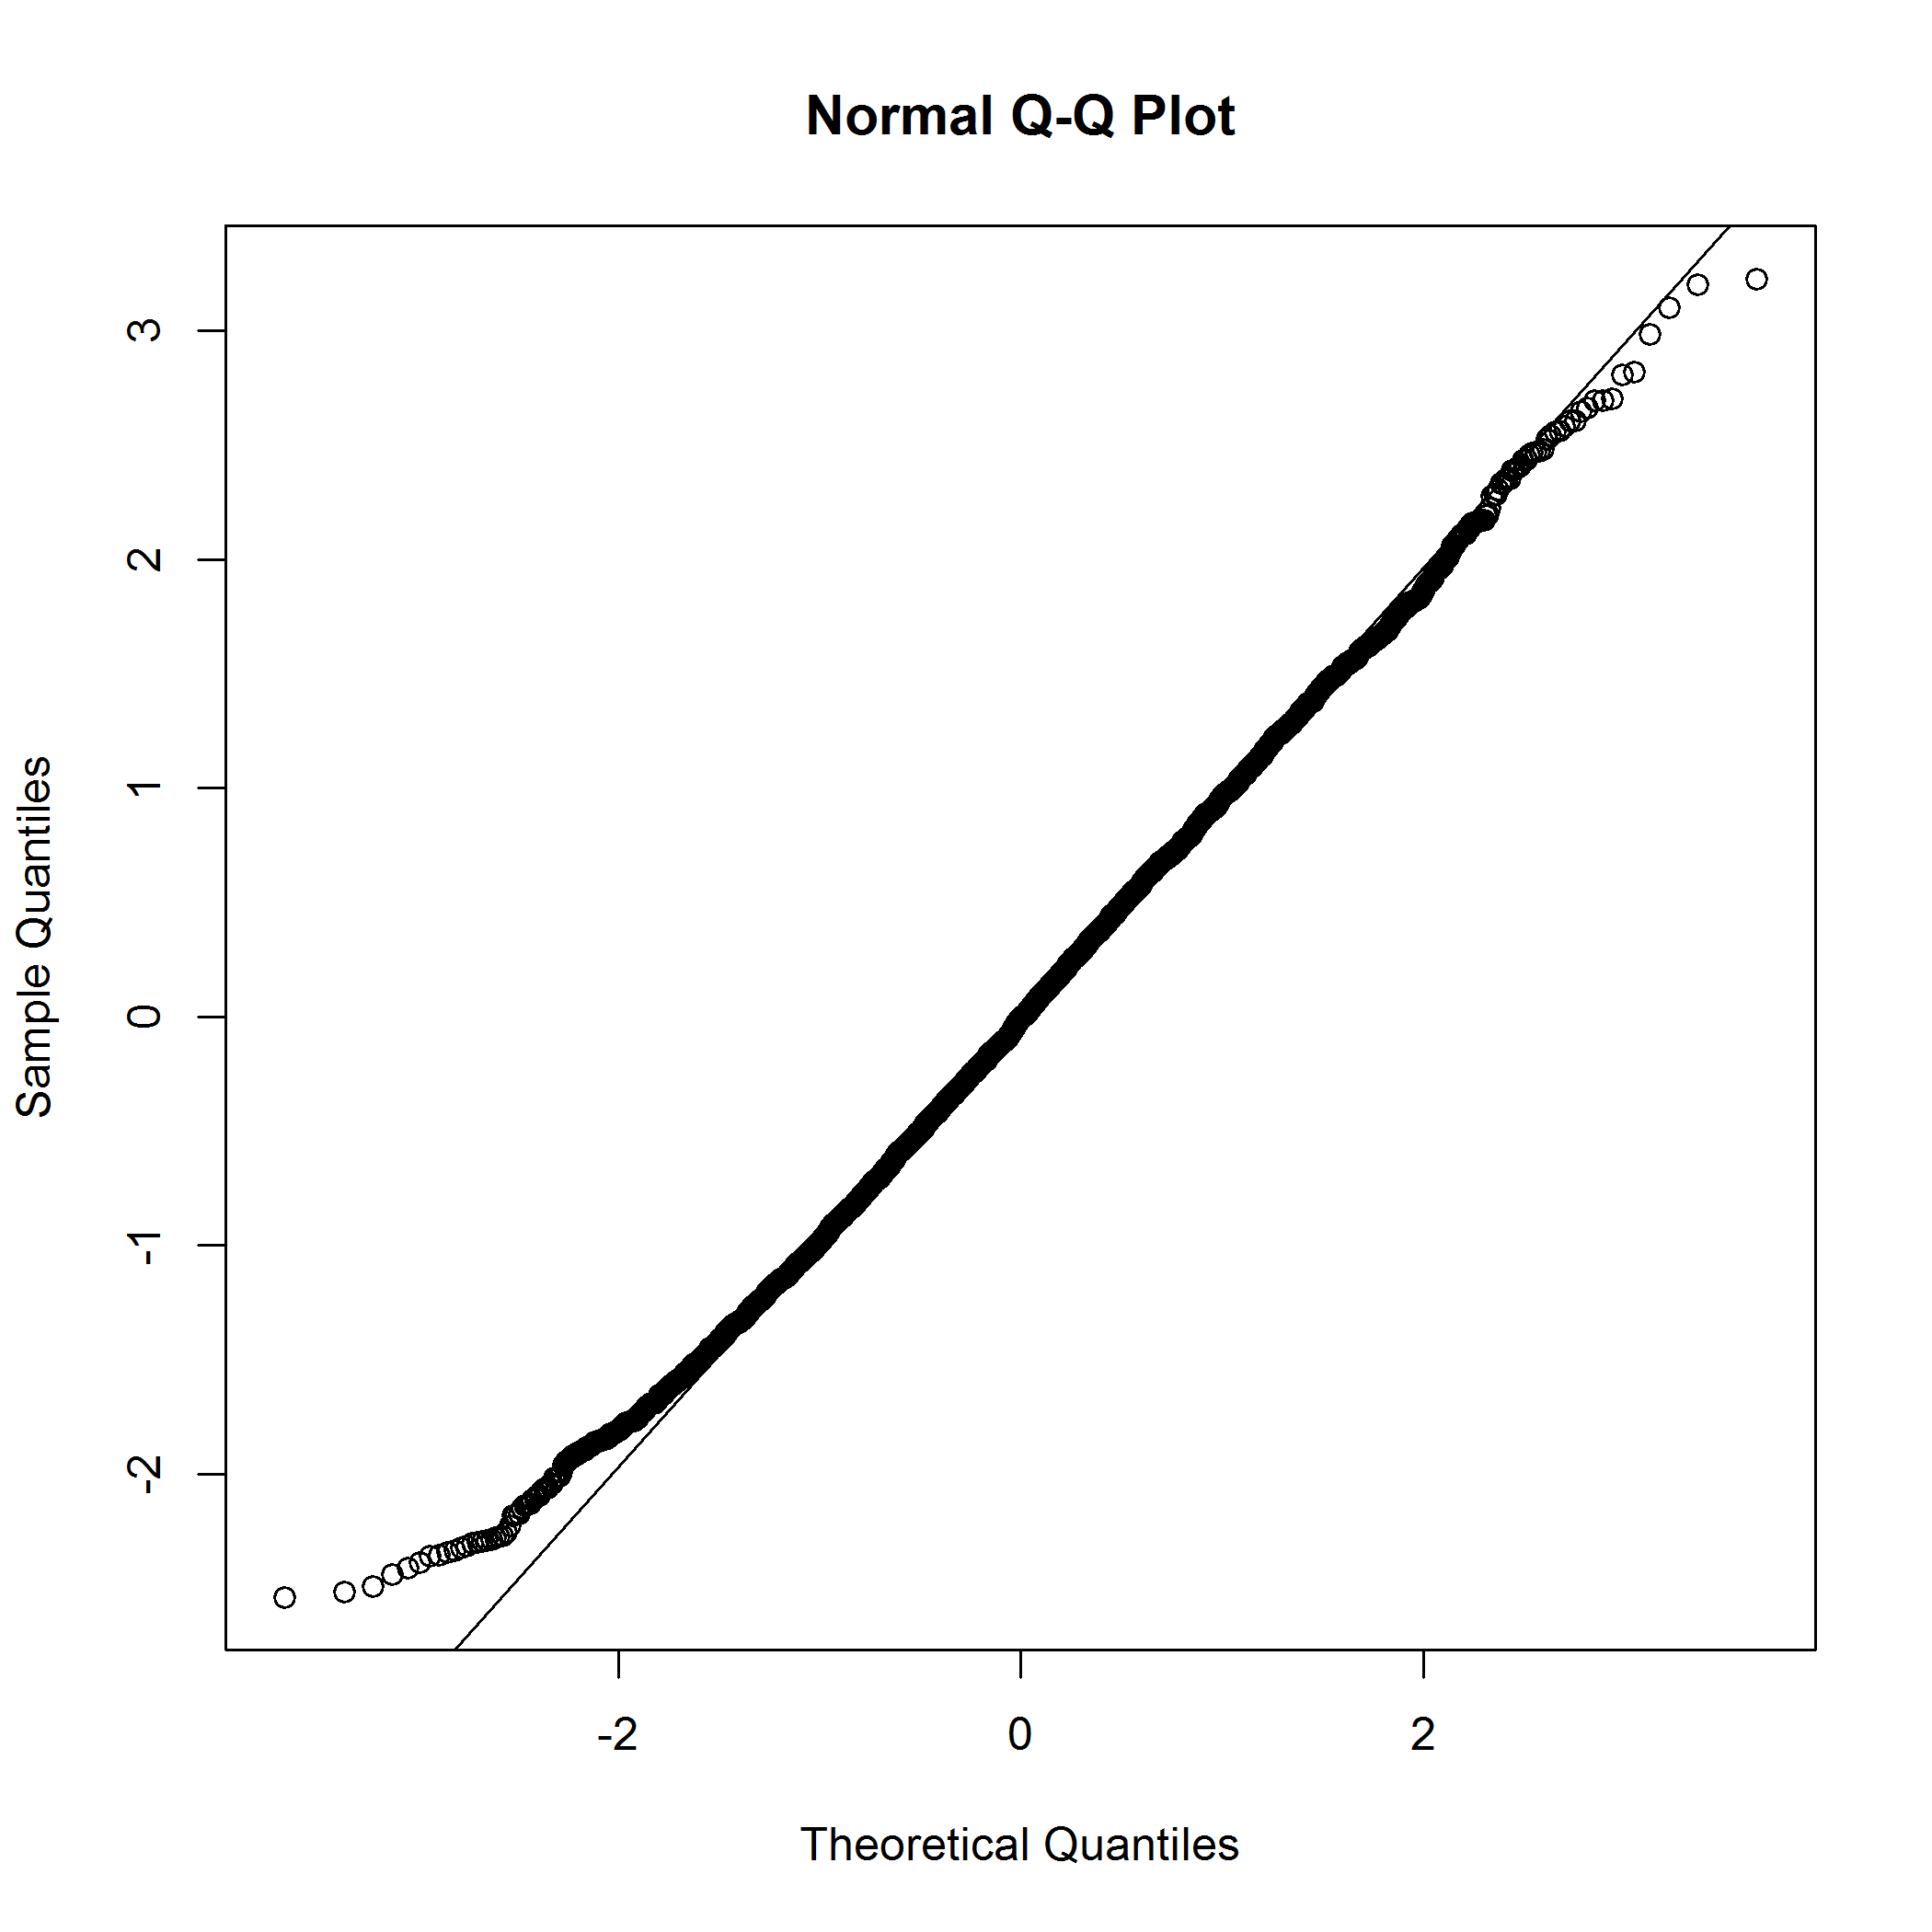
\includegraphics{Figures/Fleet12_RecPCOB_QQ.png}
\caption{Q-Q plot used to validate the goodness of fit of the lognormal
model for the CPFV onboard observer retained only catch.
\label{fig:Fleet12_RecPCOBR_QQ}}
\end{figure}

\begin{figure}[htbp]
\centering
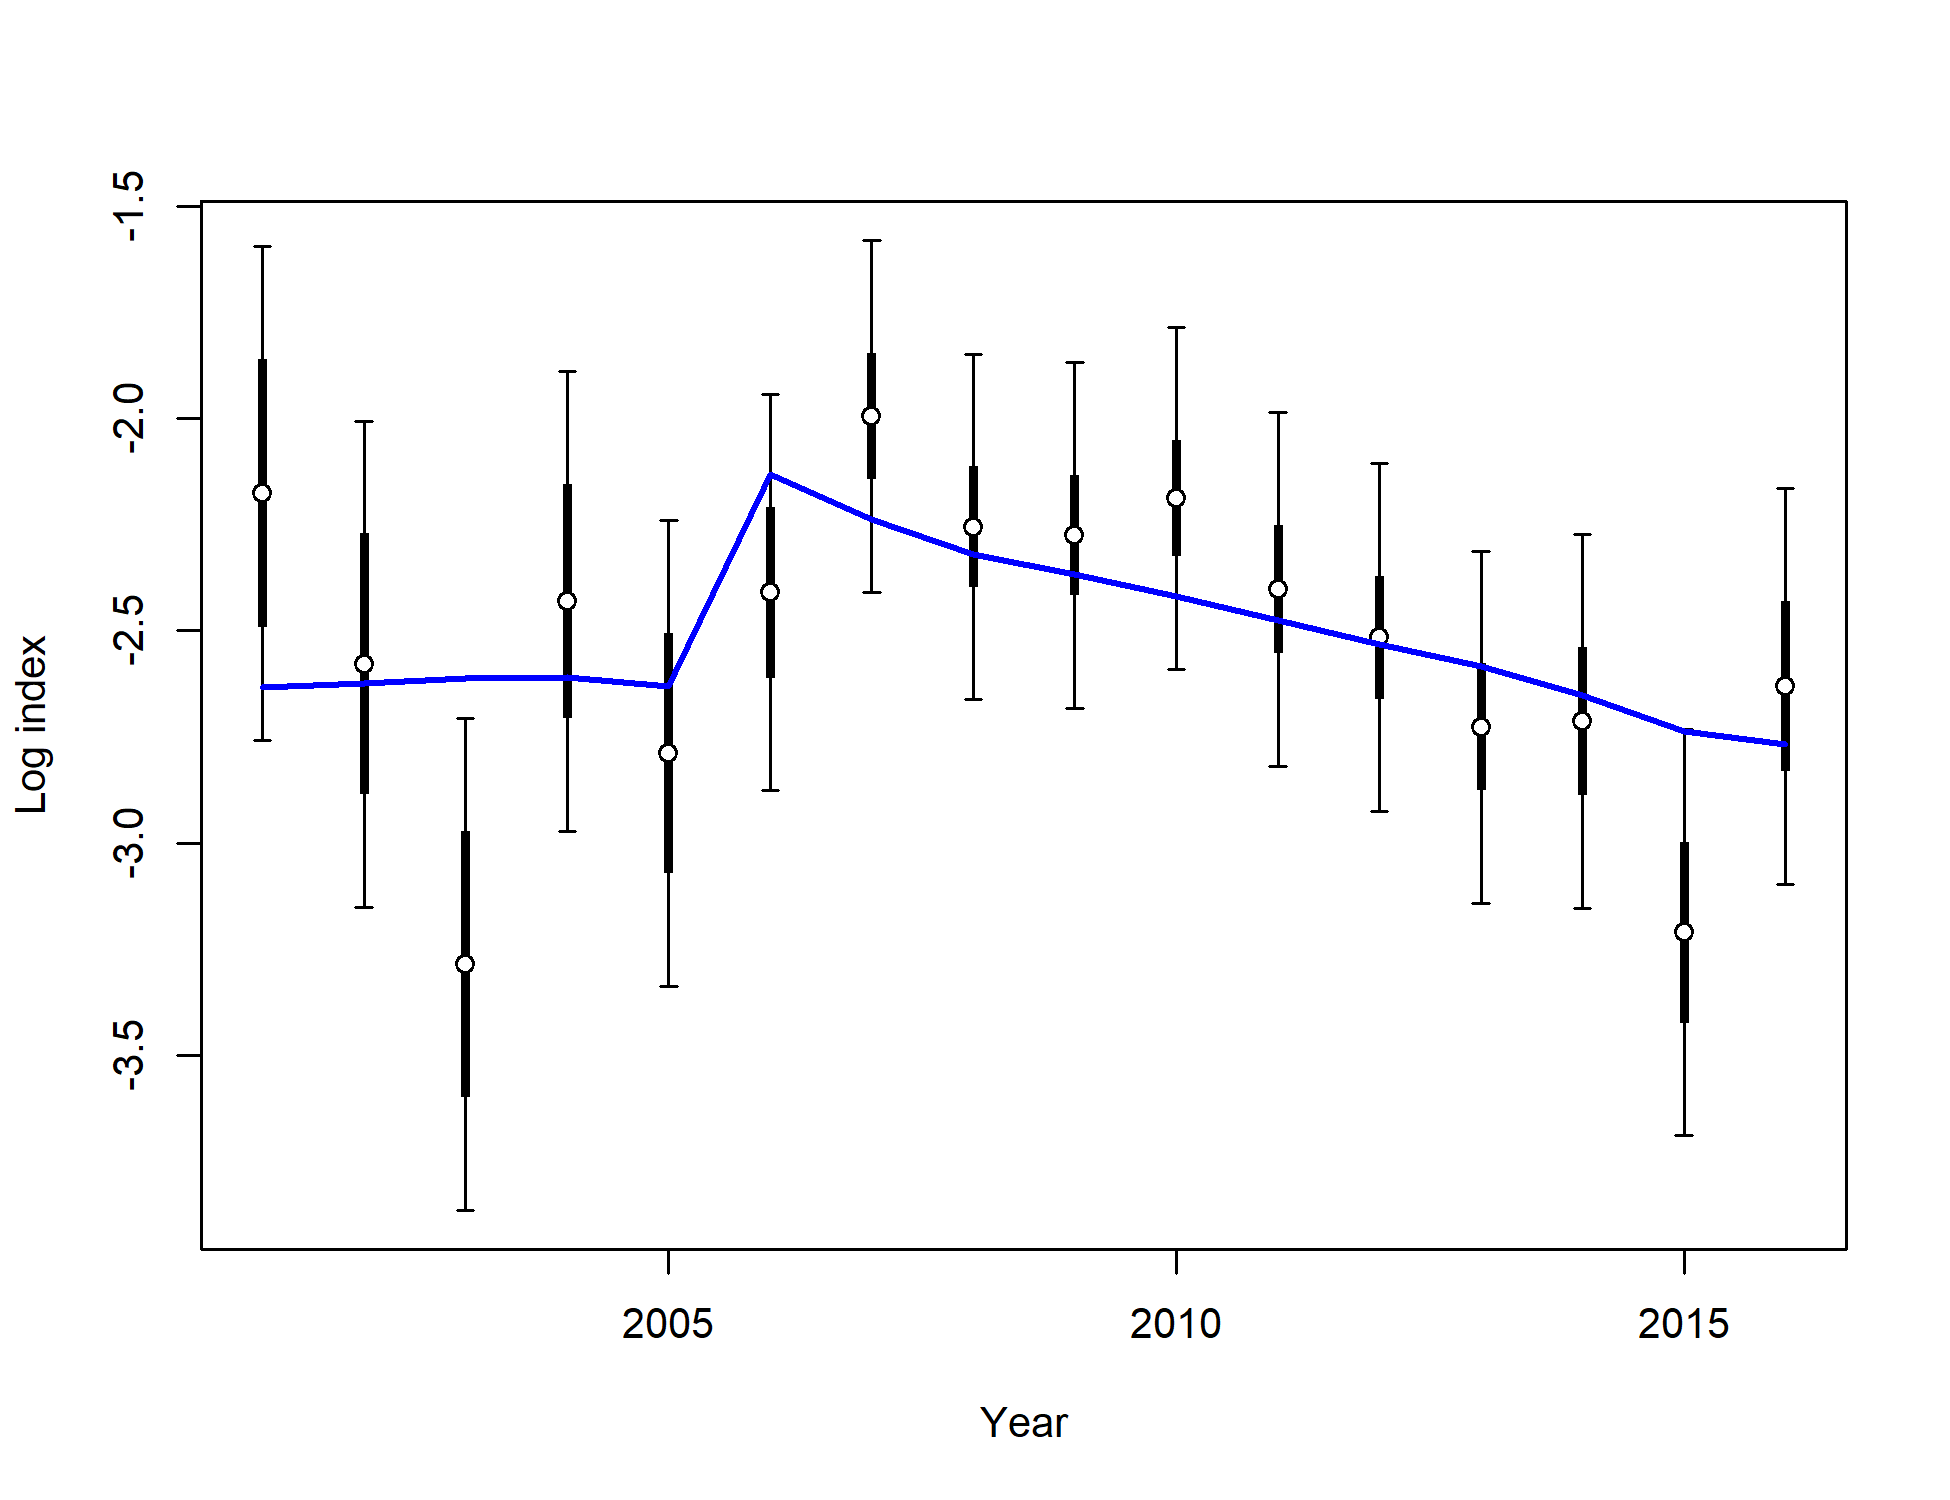
\includegraphics{r4ss/plots_mod1/index5_logcpuefit_RecPCOBR.png}
\caption{Fit to log index data on log scale for the recreational CPFV
onboard oserver retained catch index. Lines indicate 95\% uncertainty
interval around index values. Thicker lines indicate input uncertainty
before addition of estimated additional uncertainty parameter.
\label{fig:Fleet12_index5_logcpuefit_RecPCOBR}}
\end{figure}

\FloatBarrier

\begin{figure}[htbp]
\centering
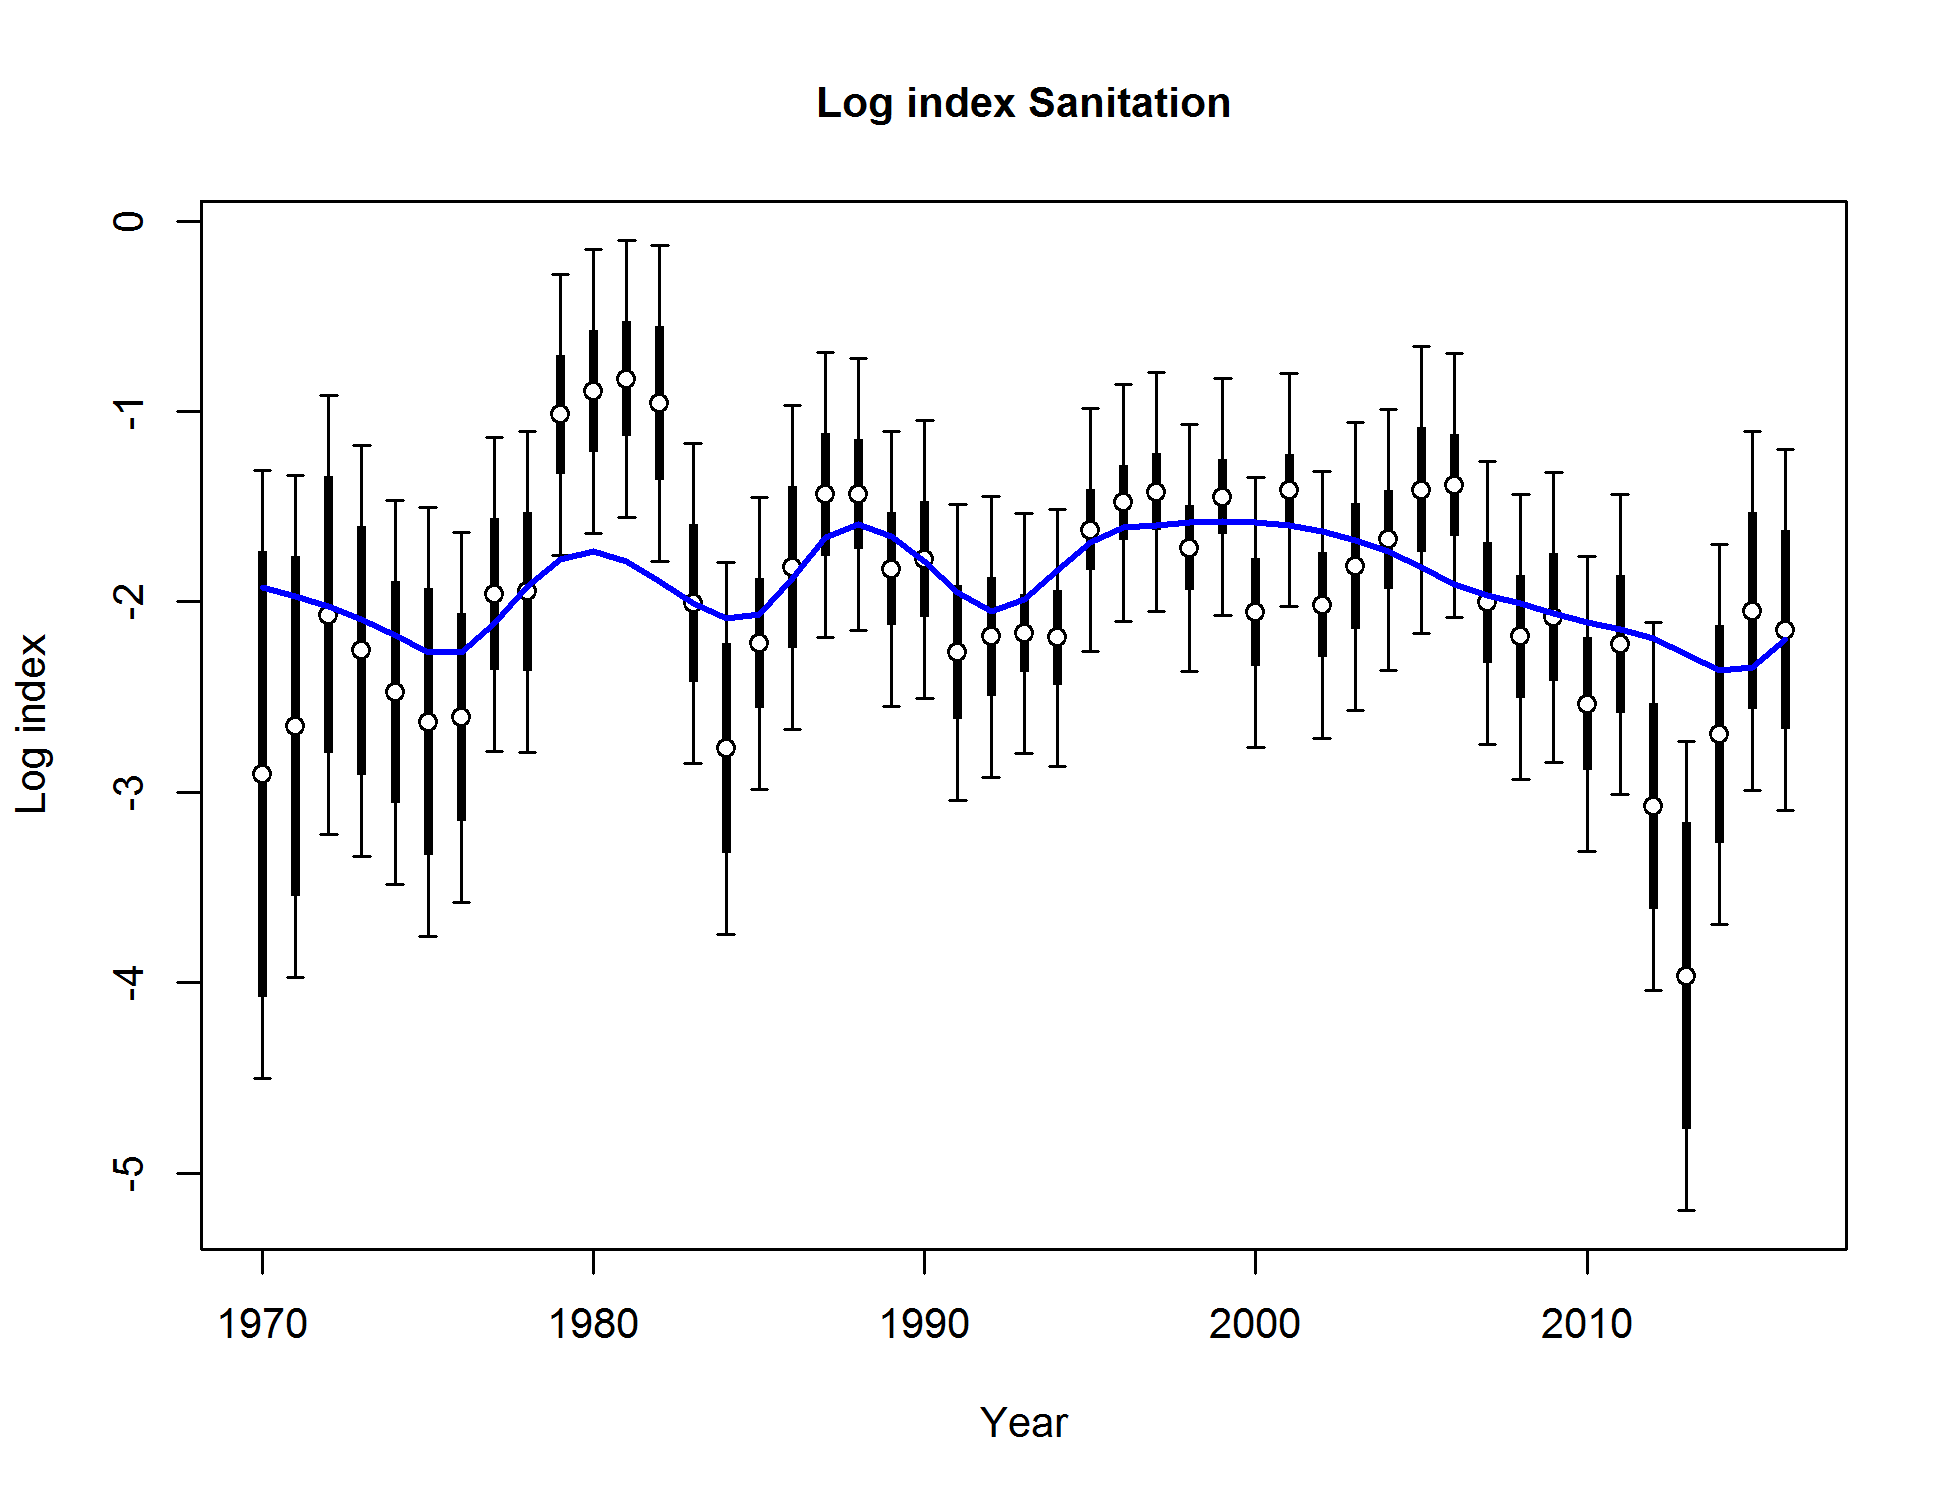
\includegraphics{r4ss/plots_mod1/index5_logcpuefit_Sanitation.png}
\caption{Fit to log index data on log scale for the recreational CPFV
onboard oserver discarded catch index. Lines indicate 95\% uncertainty
interval around index values. Thicker lines indicate input uncertainty
before addition of estimated additional uncertainty parameter.
\label{fig:index5_logcpuefit_Sanitation}}
\end{figure}

\begin{figure}[htbp]
\centering
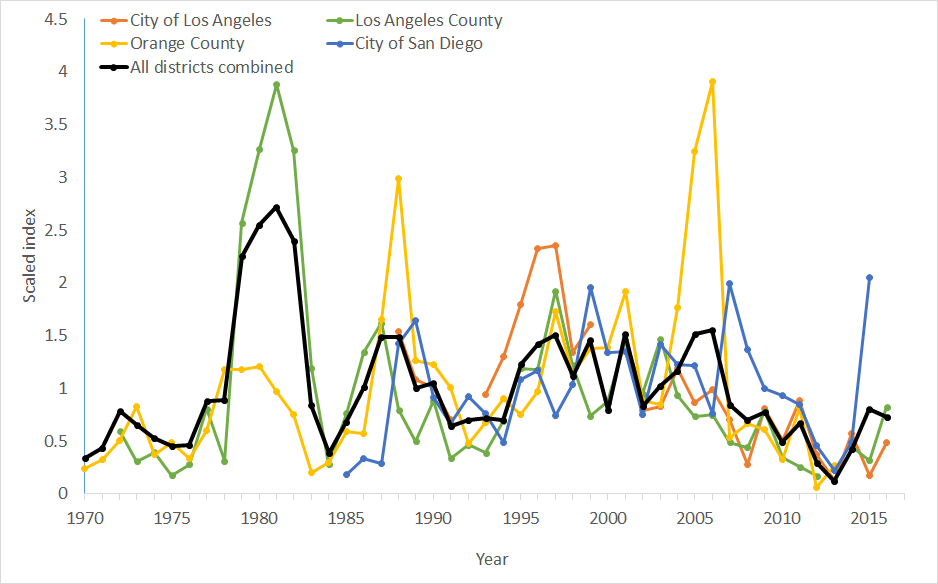
\includegraphics{Figures/Fleet7_Sanitation_indexcompare.png}
\caption{Comparison of standardized indices for each sanitation district
independently and with data from all sanitation districts combined.
\label{fig:Fleet7_Sanitation_indexcompare}}
\end{figure}

\begin{figure}[htbp]
\centering
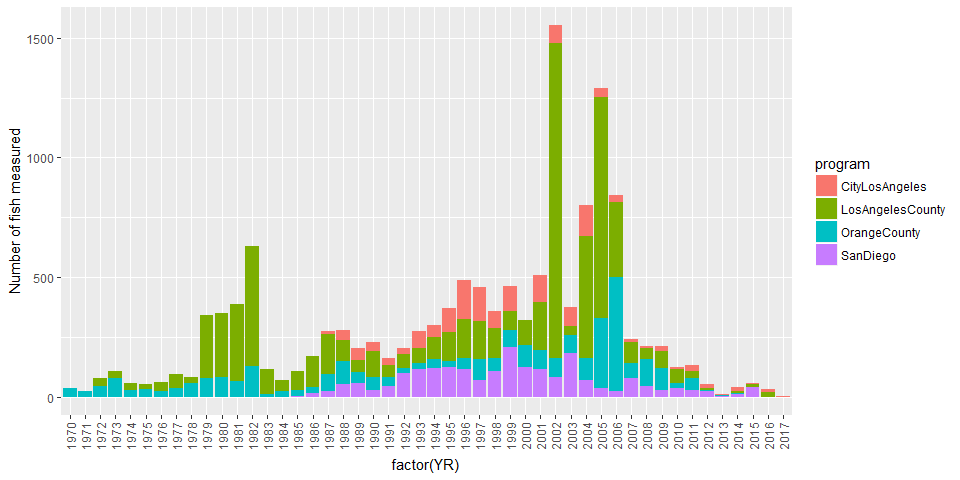
\includegraphics{Figures/Fleet7_Sanitation_length_source.png}
\caption{Sample sizes of measured California scorpionfish by sanitation
district and year. \label{fig:Fleet7_Sanitation_lengthbydistrict}}
\end{figure}

\begin{figure}[htbp]
\centering
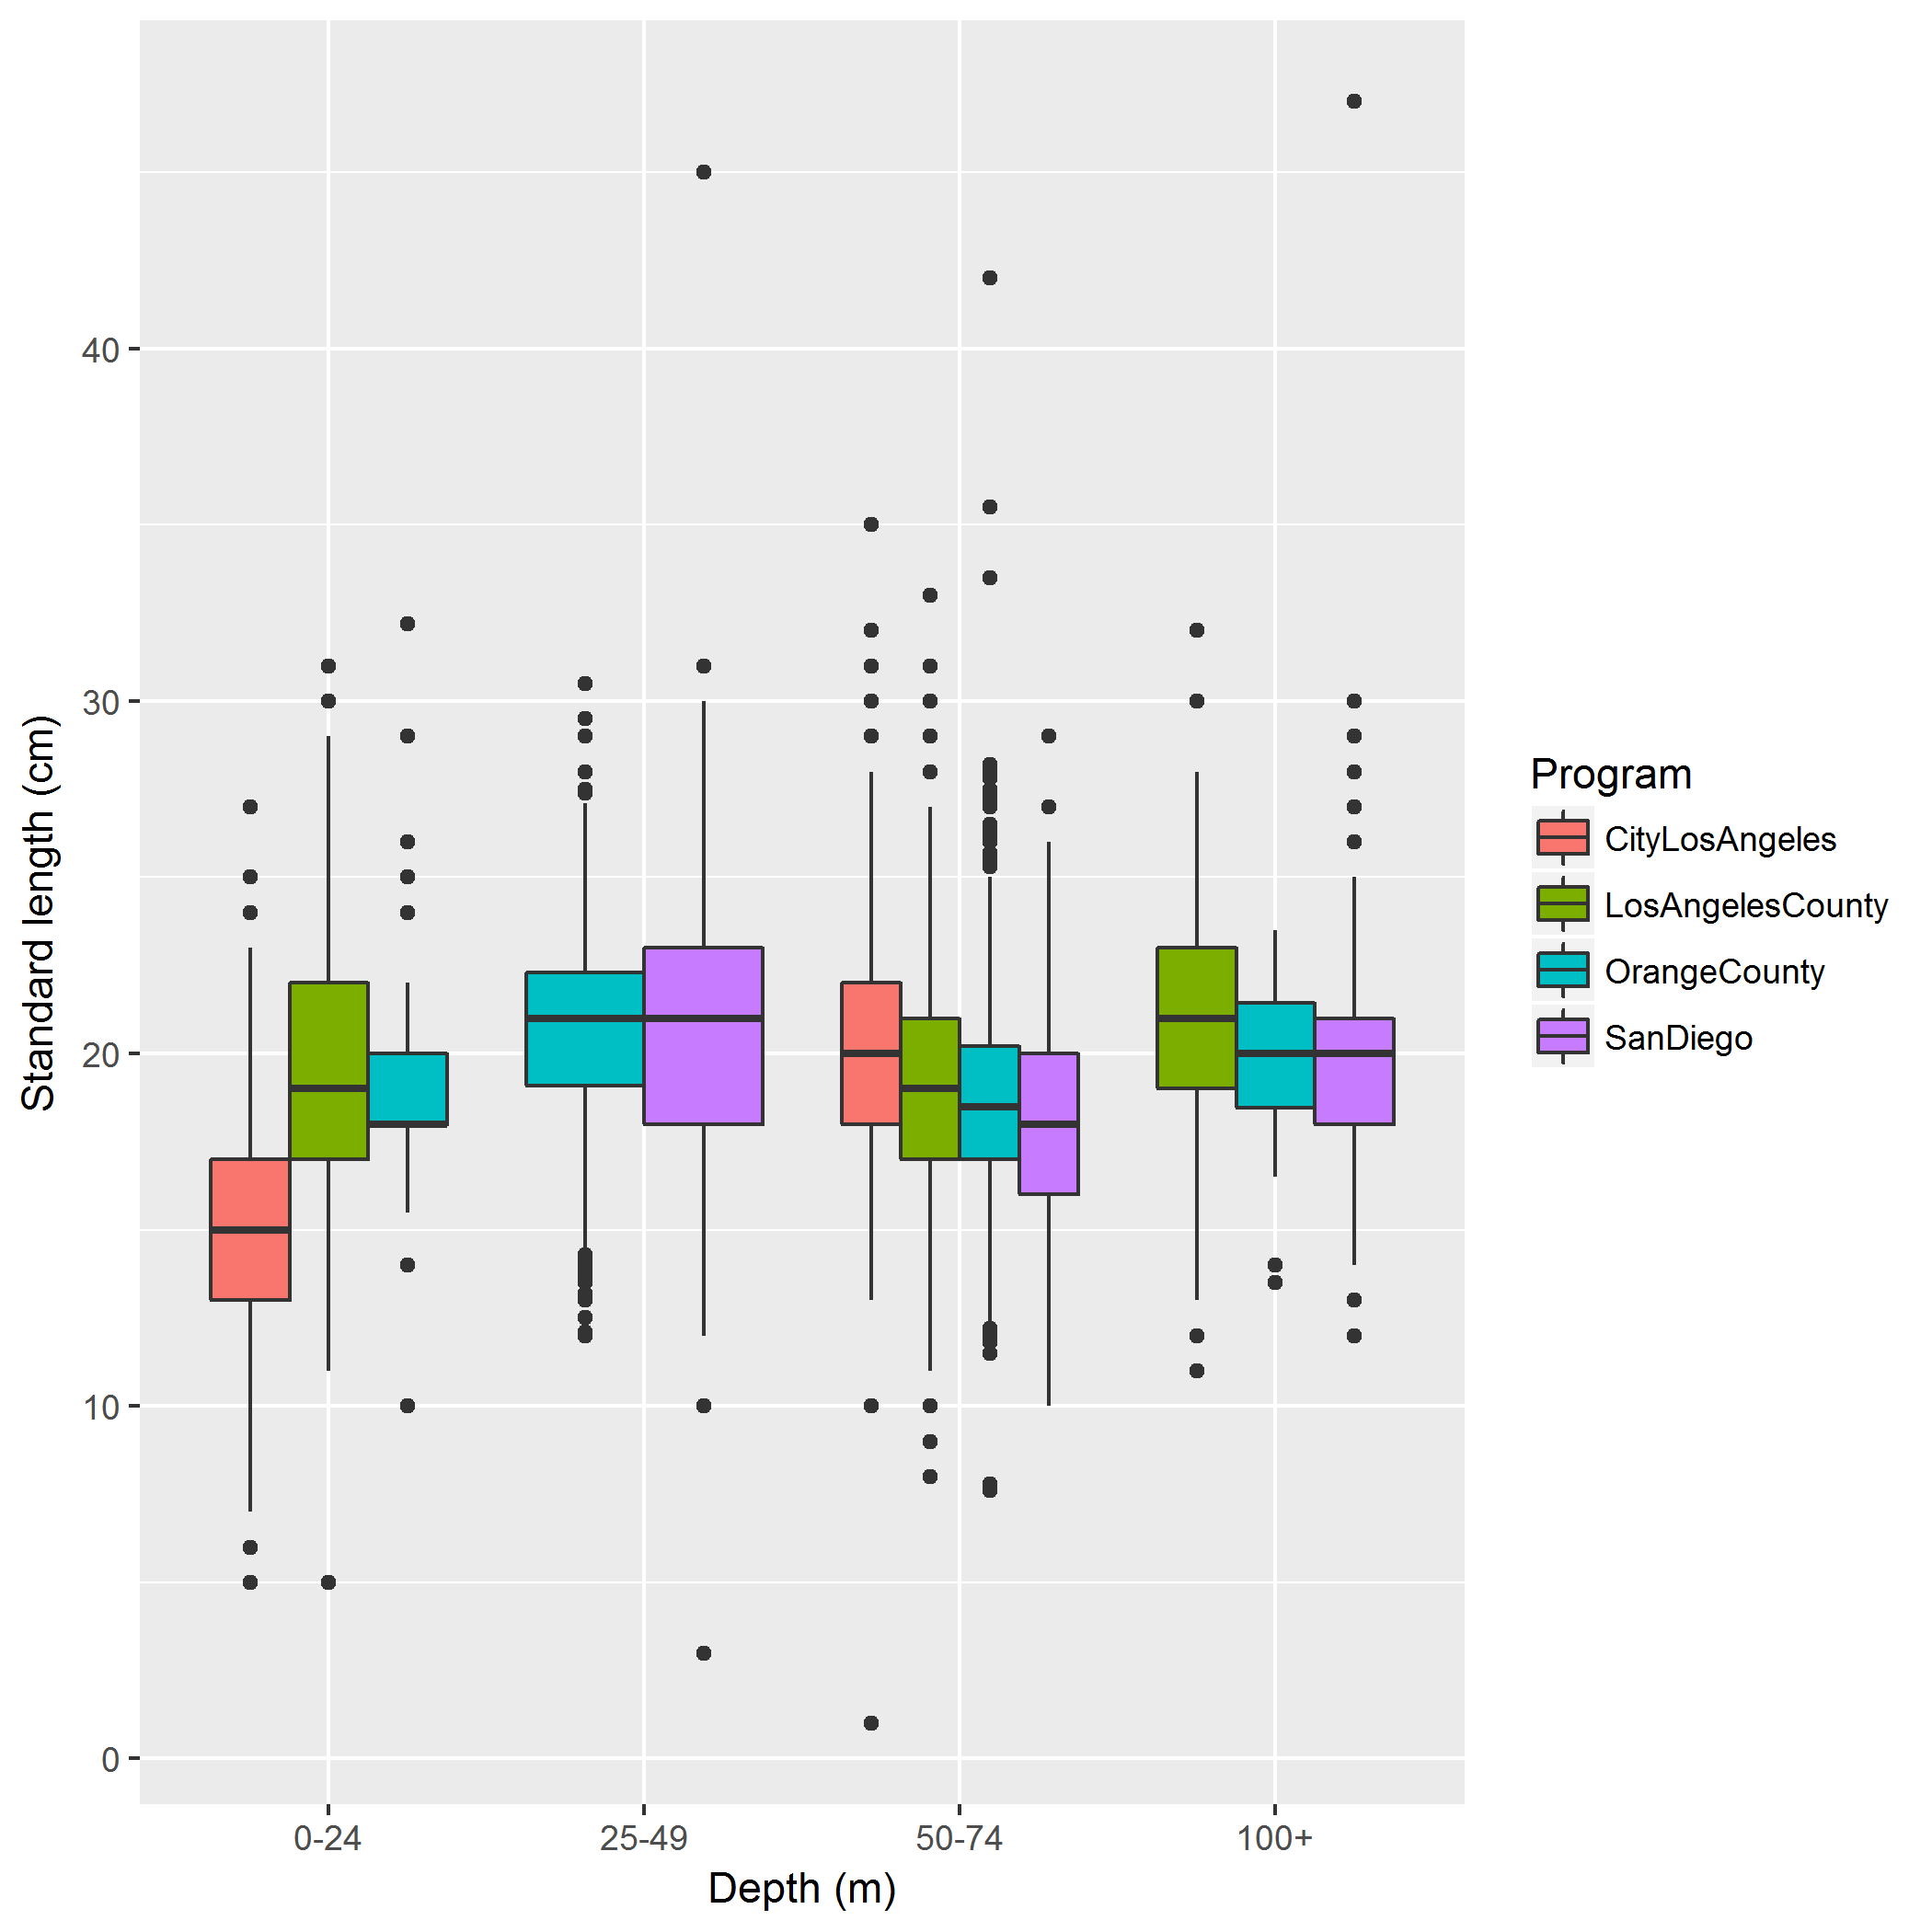
\includegraphics{Figures/Fleet7_Sanitation_lengthboxplots.png}
\caption{Boxplots of measured California scorpionfish from the
sanitation district surveys by program and 25 m depth bins.
\label{fig:Fleet7_Sanitation_lengthboxplots}}
\end{figure}

\begin{figure}[htbp]
\centering
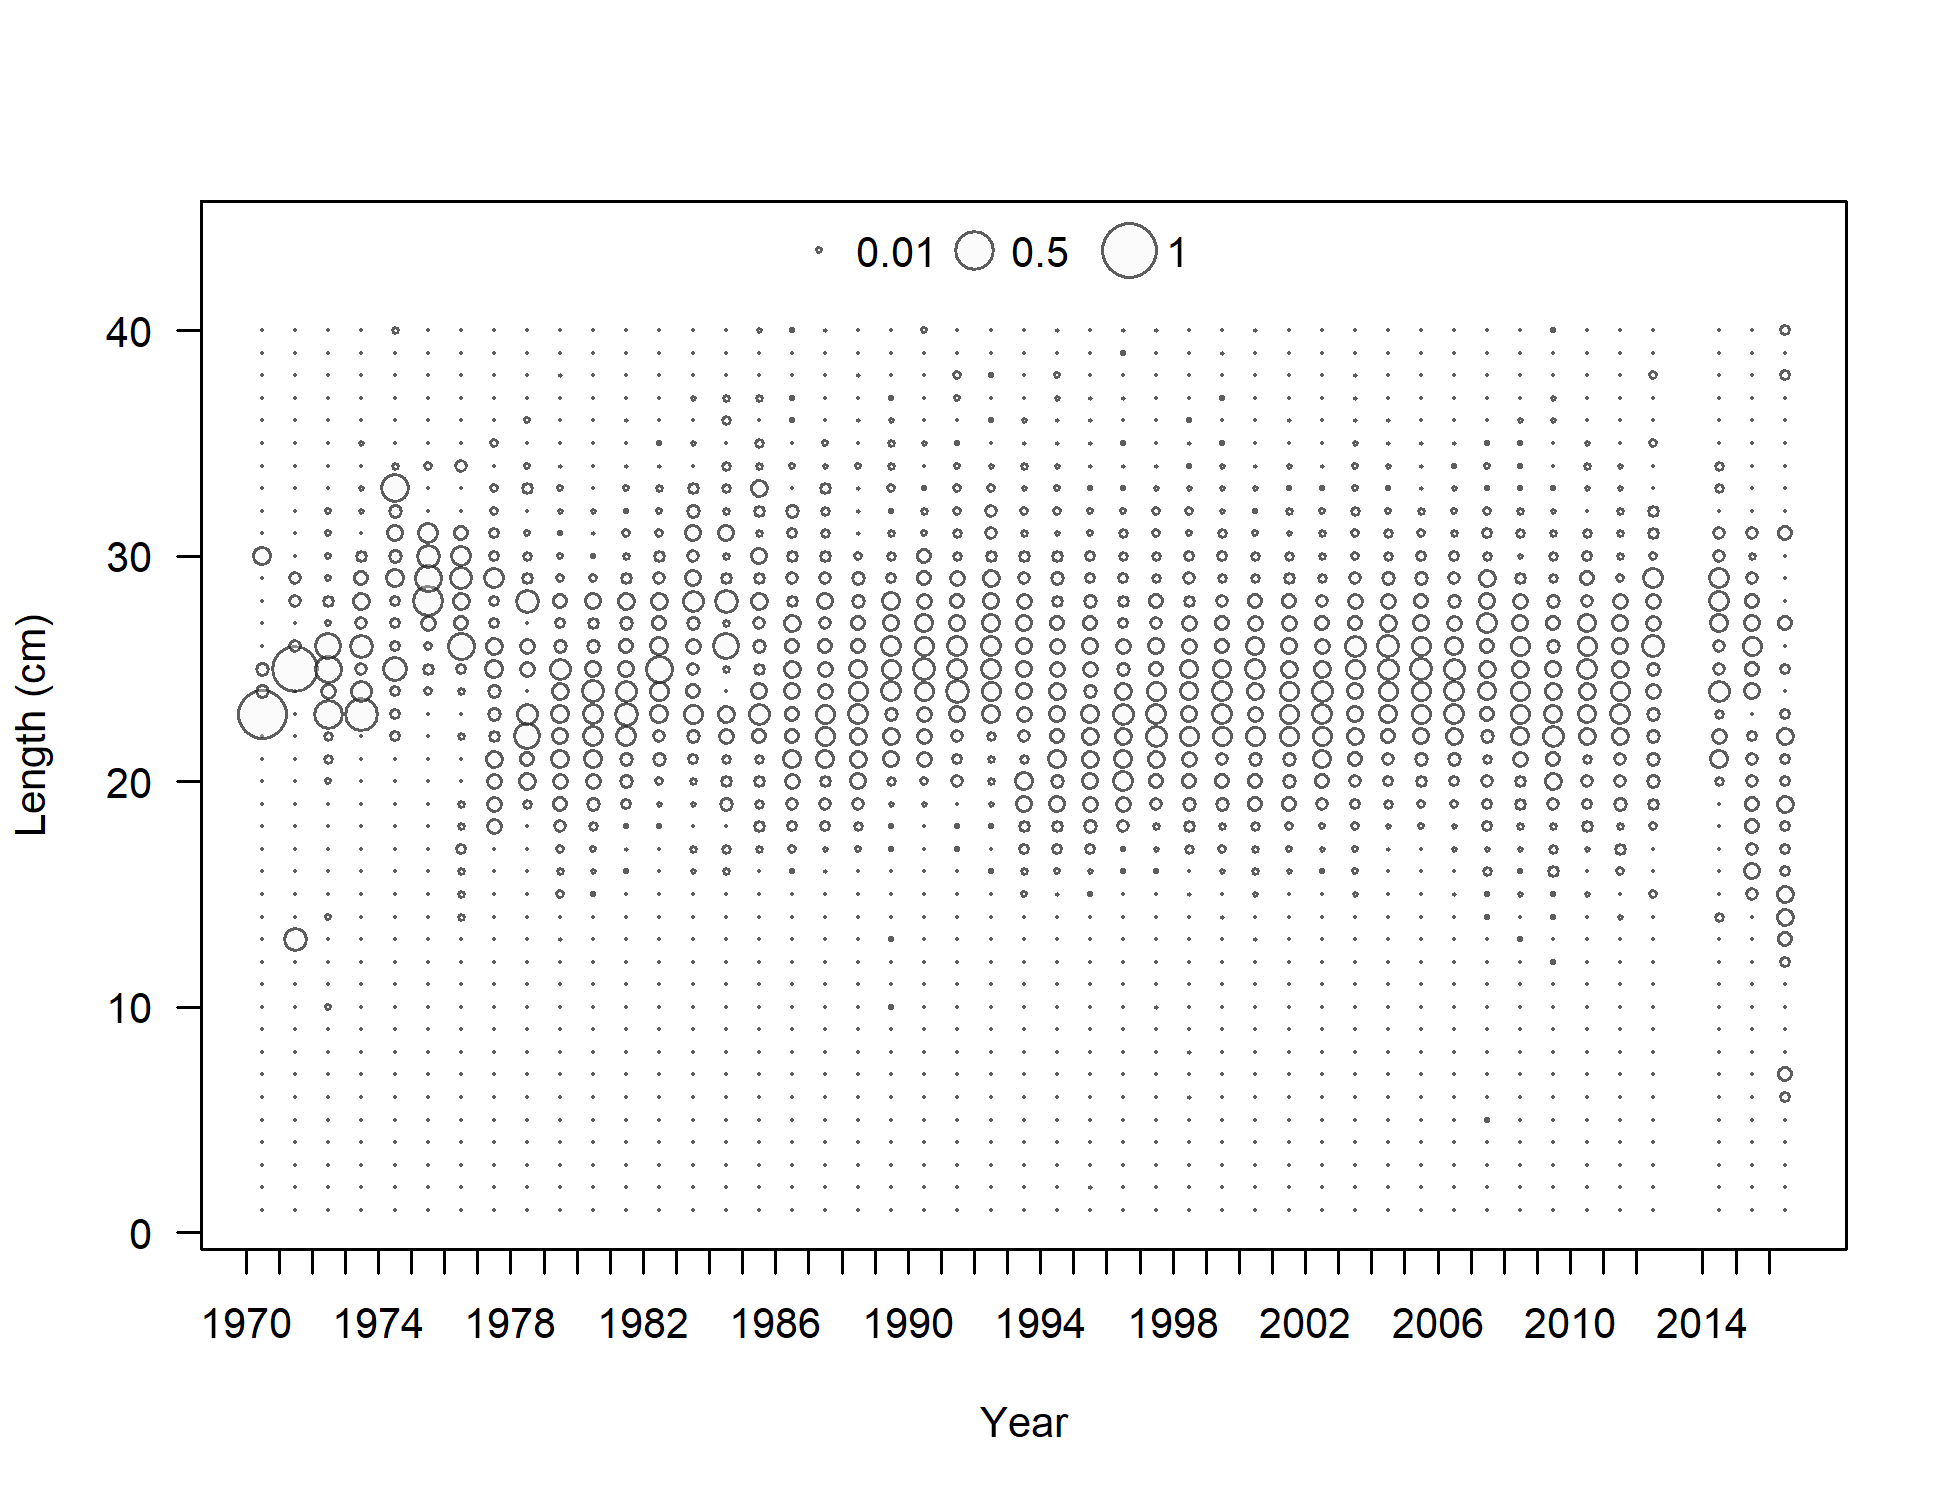
\includegraphics{r4ss/plots_mod1/comp_lendat_bubflt7mkt2_page2.png}
\caption{Length frequency distributions from the sanitation disricts
trawl surveys. \label{fig:Fleet7_comp_lendat_bubflt10mkt2}}
\end{figure}

\FloatBarrier

\begin{figure}[htbp]
\centering
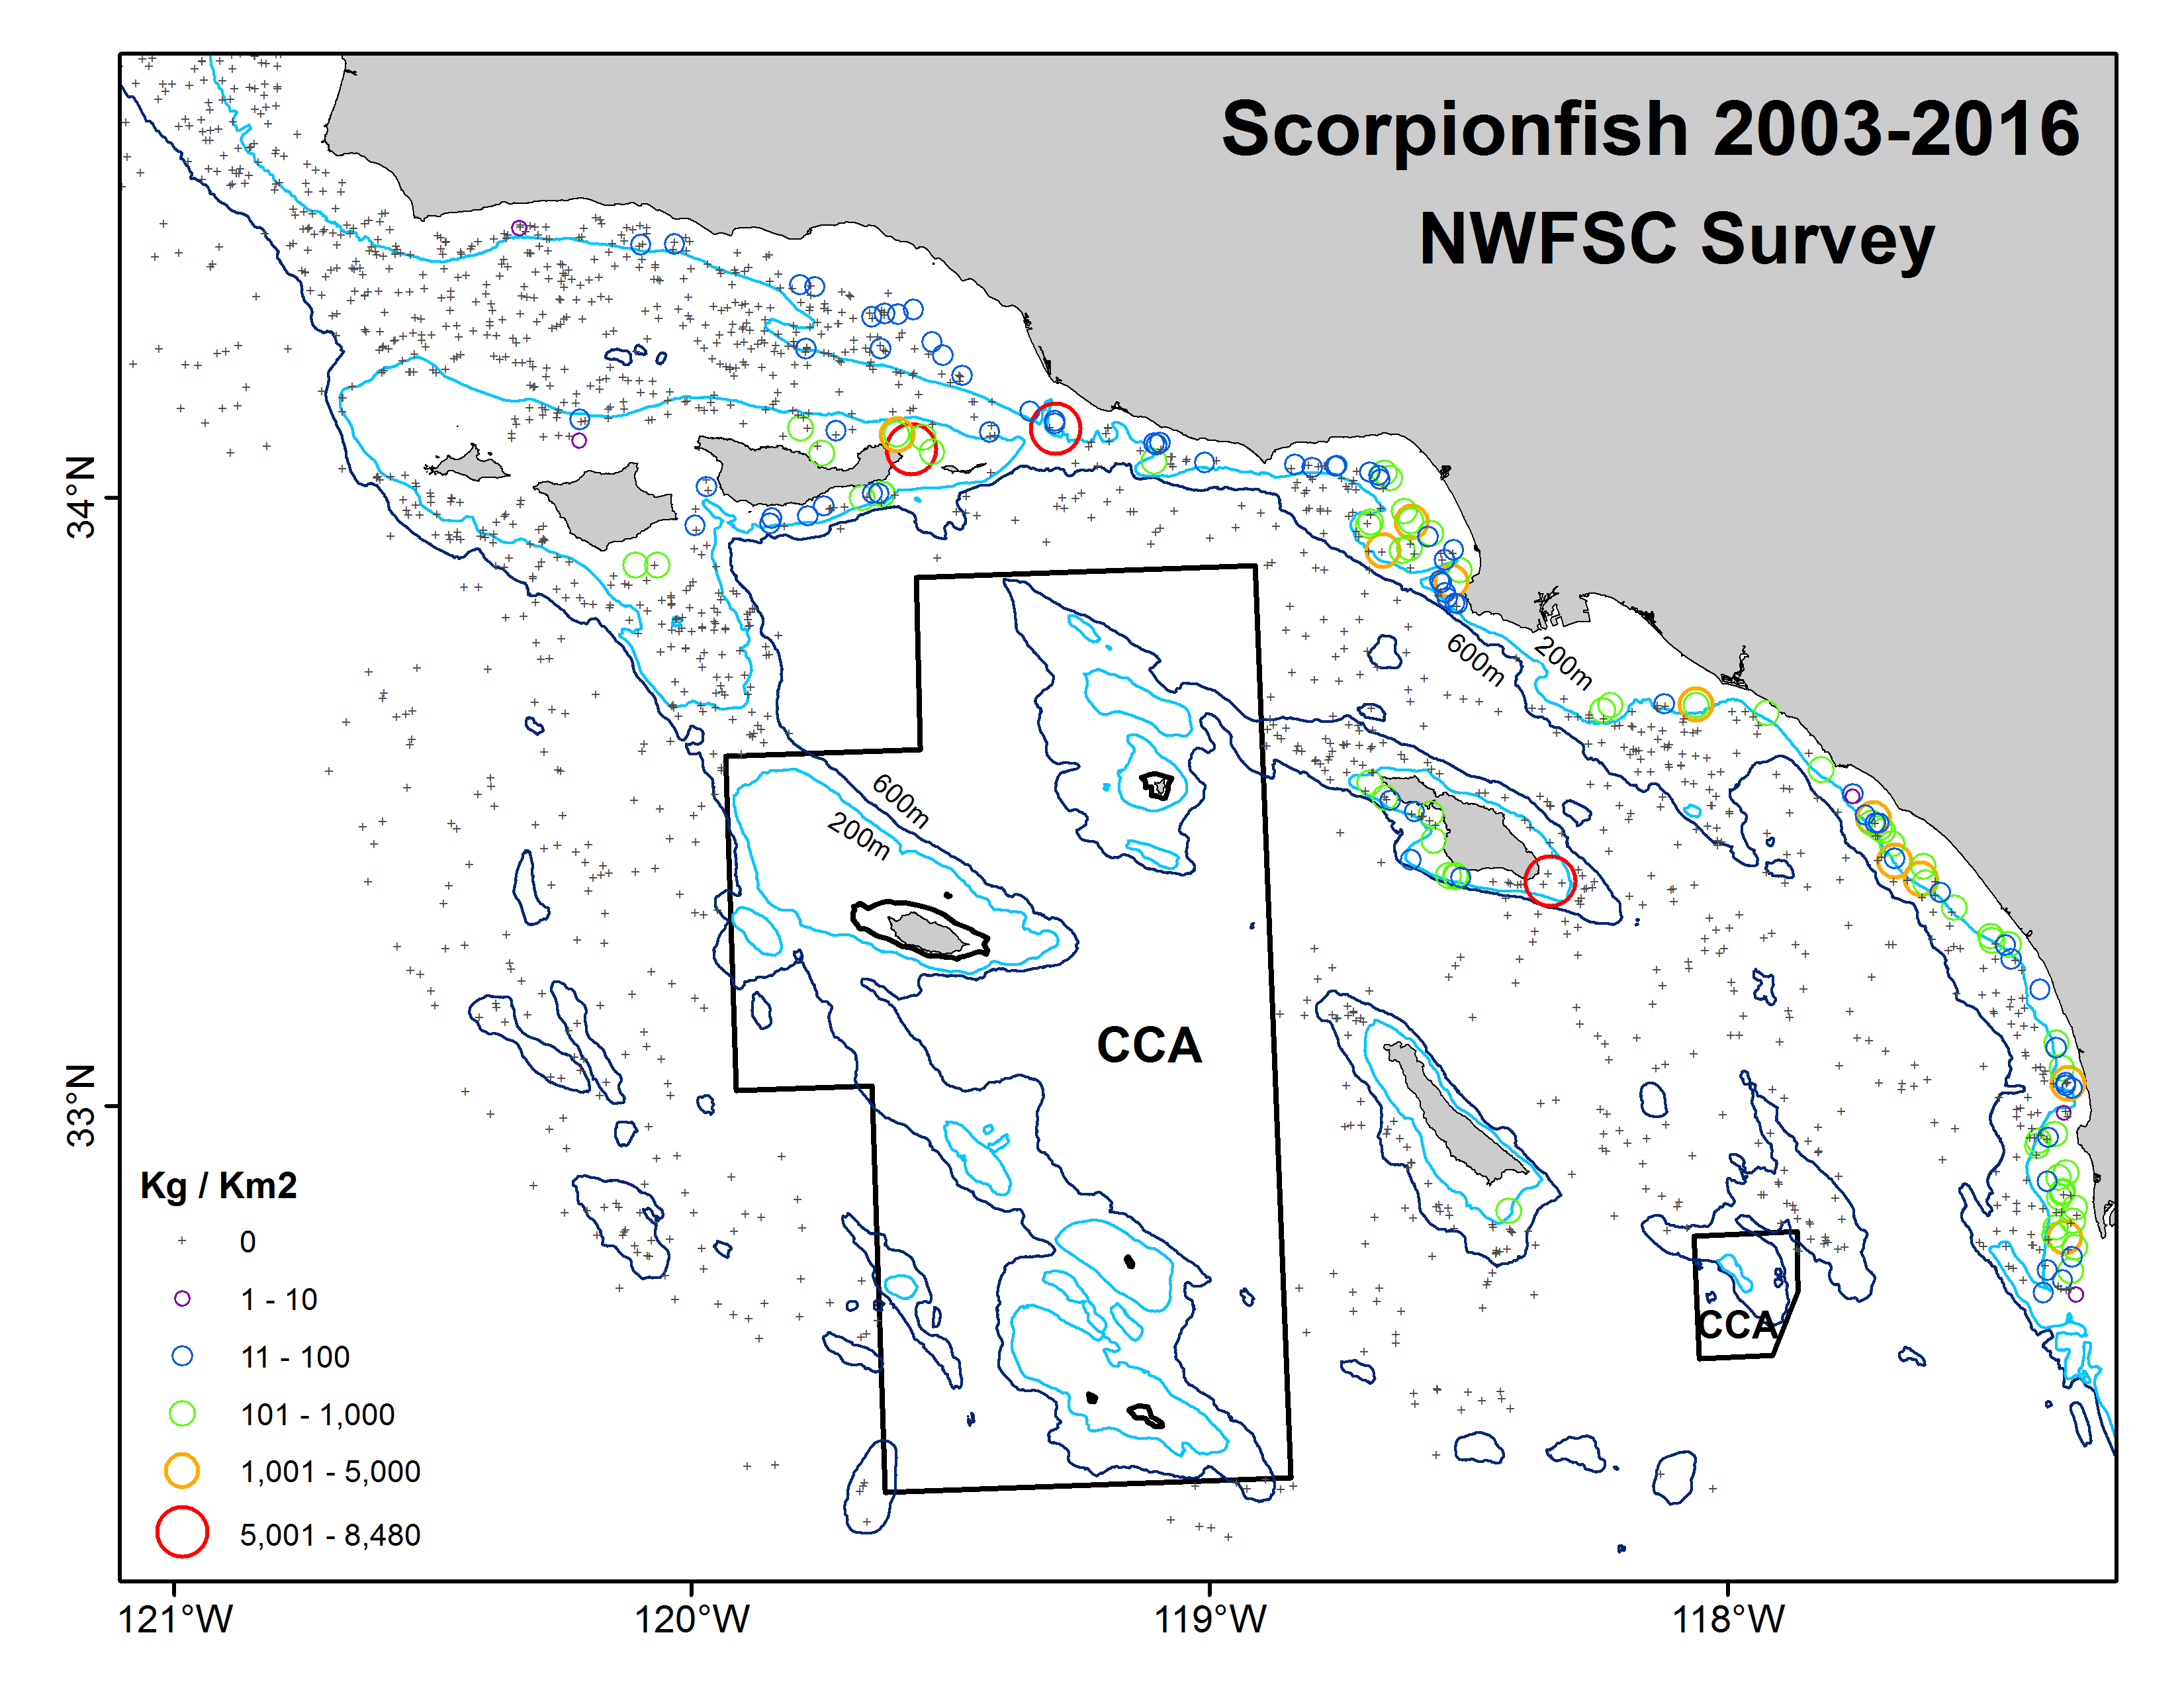
\includegraphics{Figures/NWFSCtrawl_map.png}
\caption{Spatial distribution of raw catch rates of Scorpionfish from
NWFSC trawl survey between 2003 and 2016. Depth contour lines of 200m
and 600m and the CAC areas are shown. Note that sizes and colors of
circles represent catch rate in log scales (Credit of Rebecca Miller,
SWFSC). \label{fig:Fleet8_NWFSCtrawl_map}}
\end{figure}

\begin{figure}[htbp]
\centering
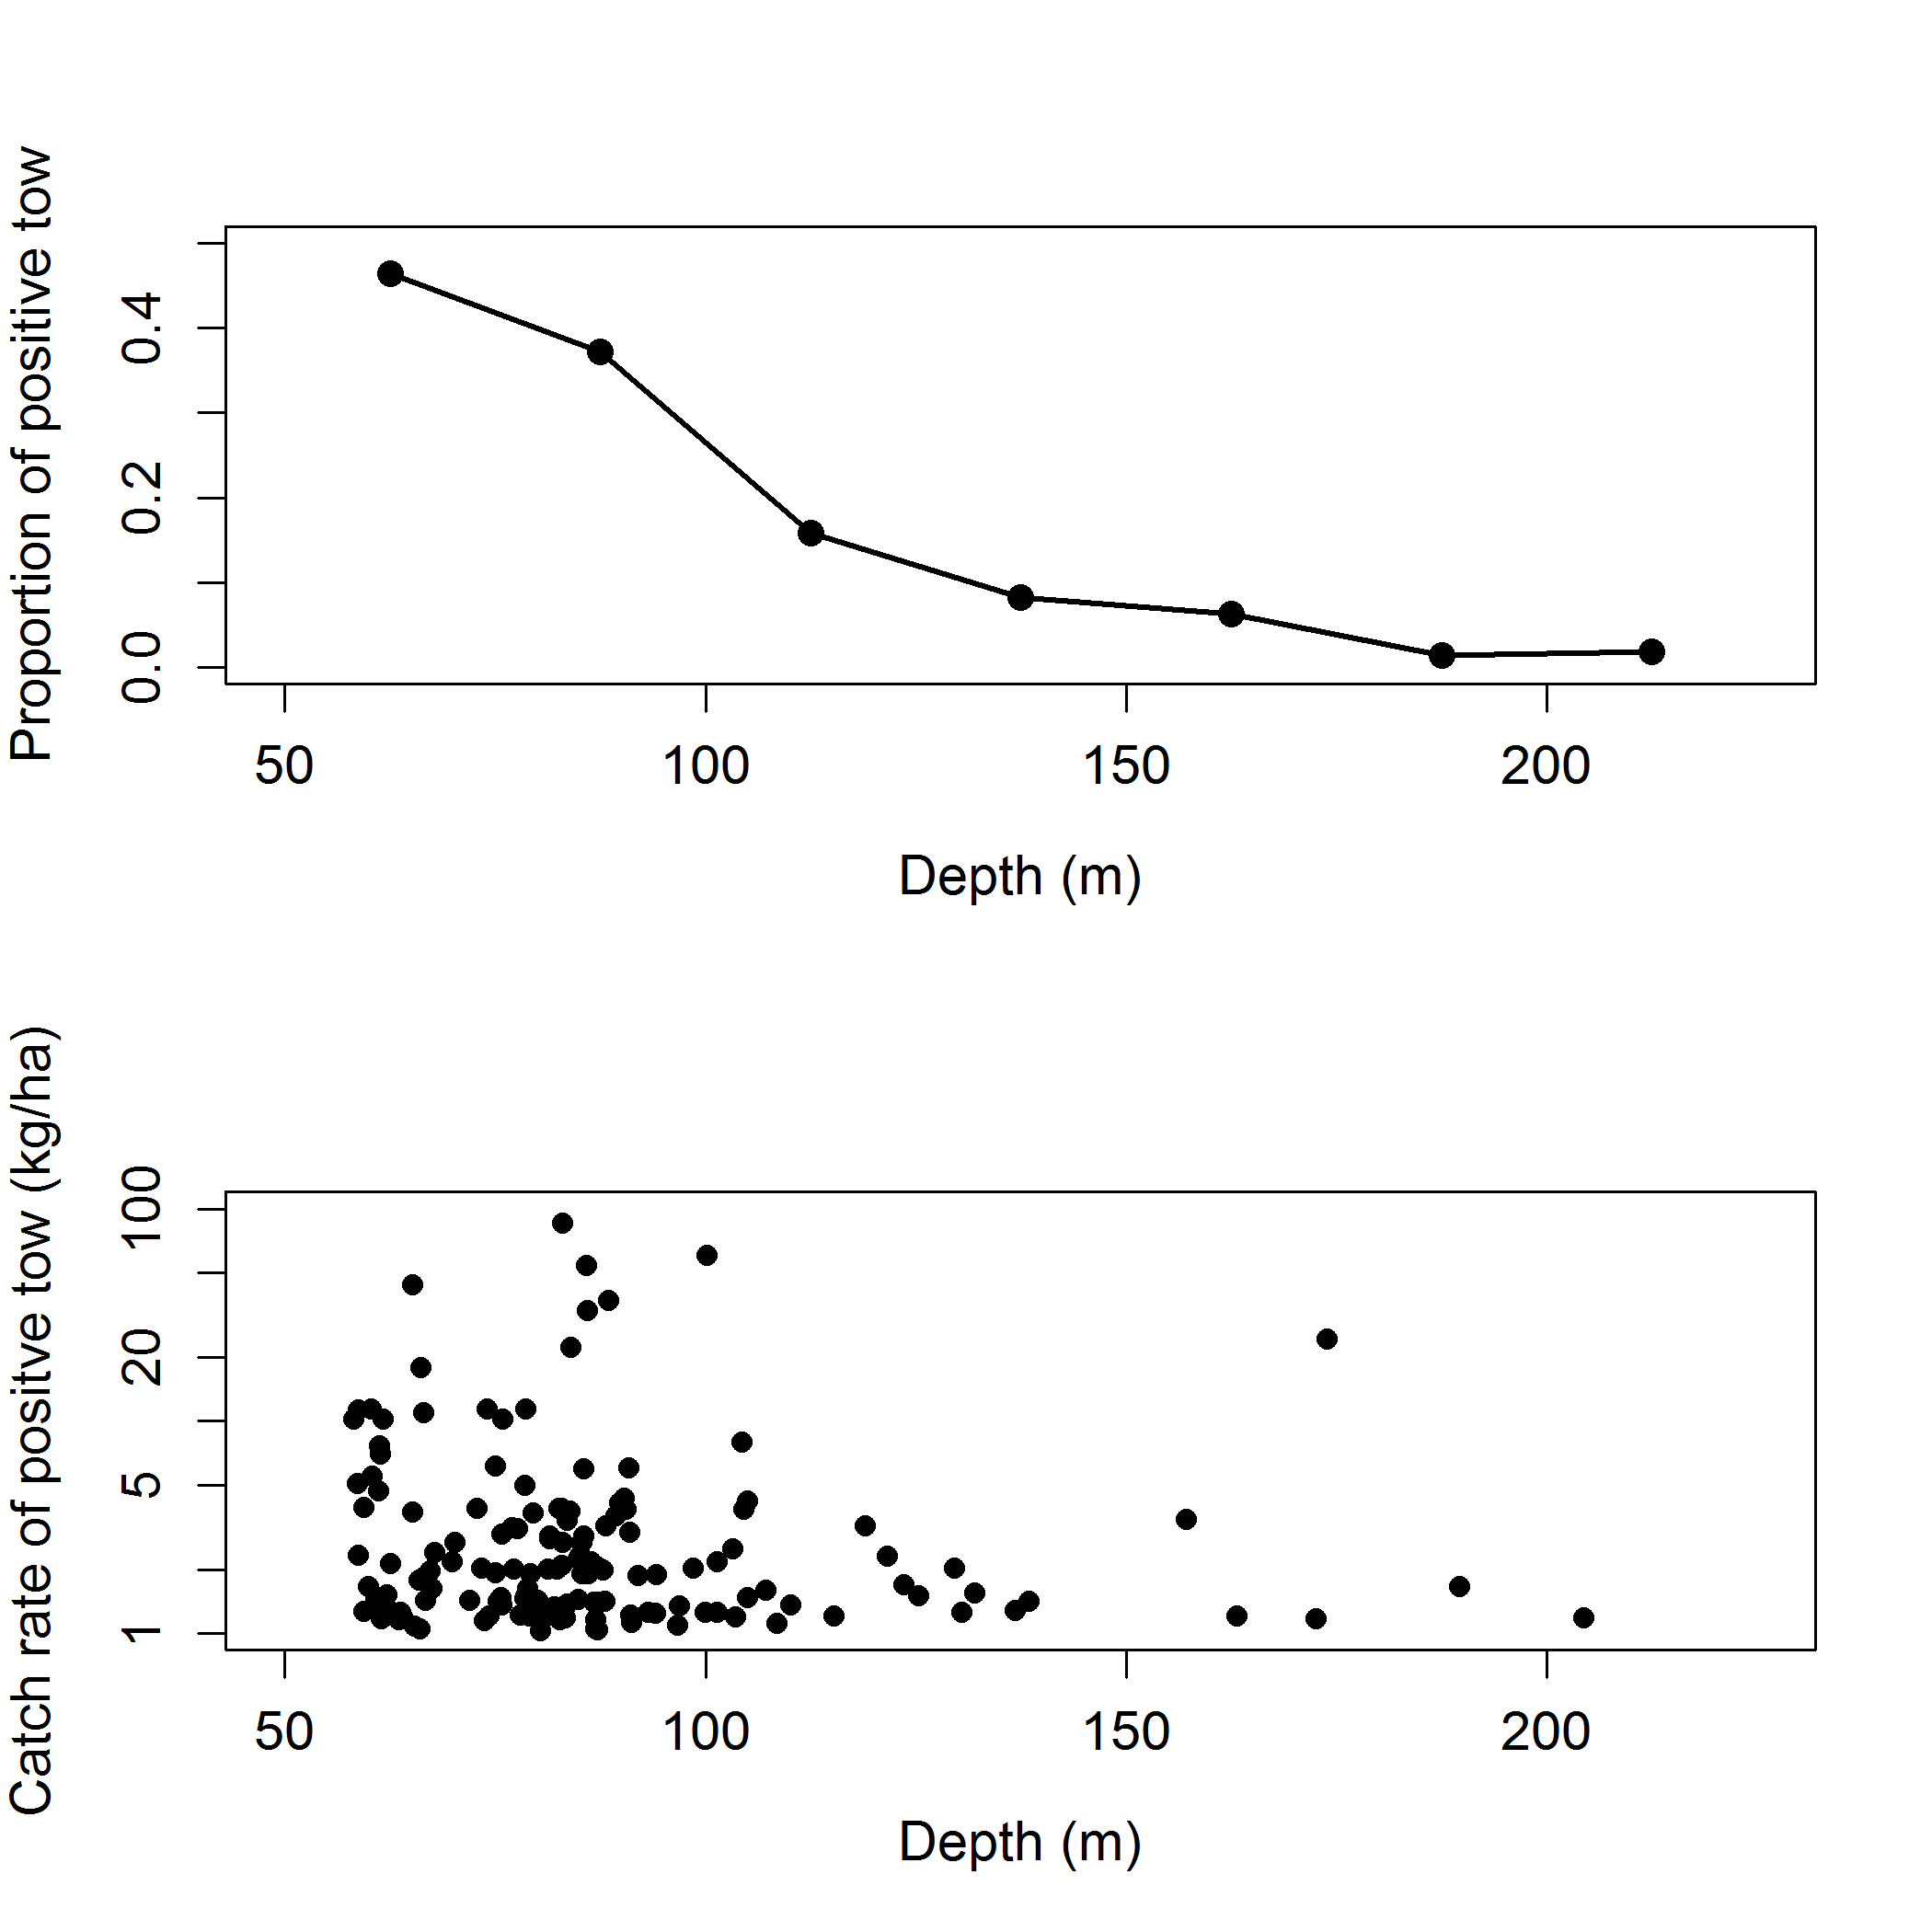
\includegraphics{Figures/NWFSCtrawl_posdepth.png}
\caption{Plots of the proportion of positive tows (top panel) and the
raw catch rates of positive tows (bottom panel) by depth zones (25 m
interval) for NWFSC trawl survey.
\label{fig:Fleet8_NWFSCtrawl_posdepth}}
\end{figure}

\begin{figure}[htbp]
\centering
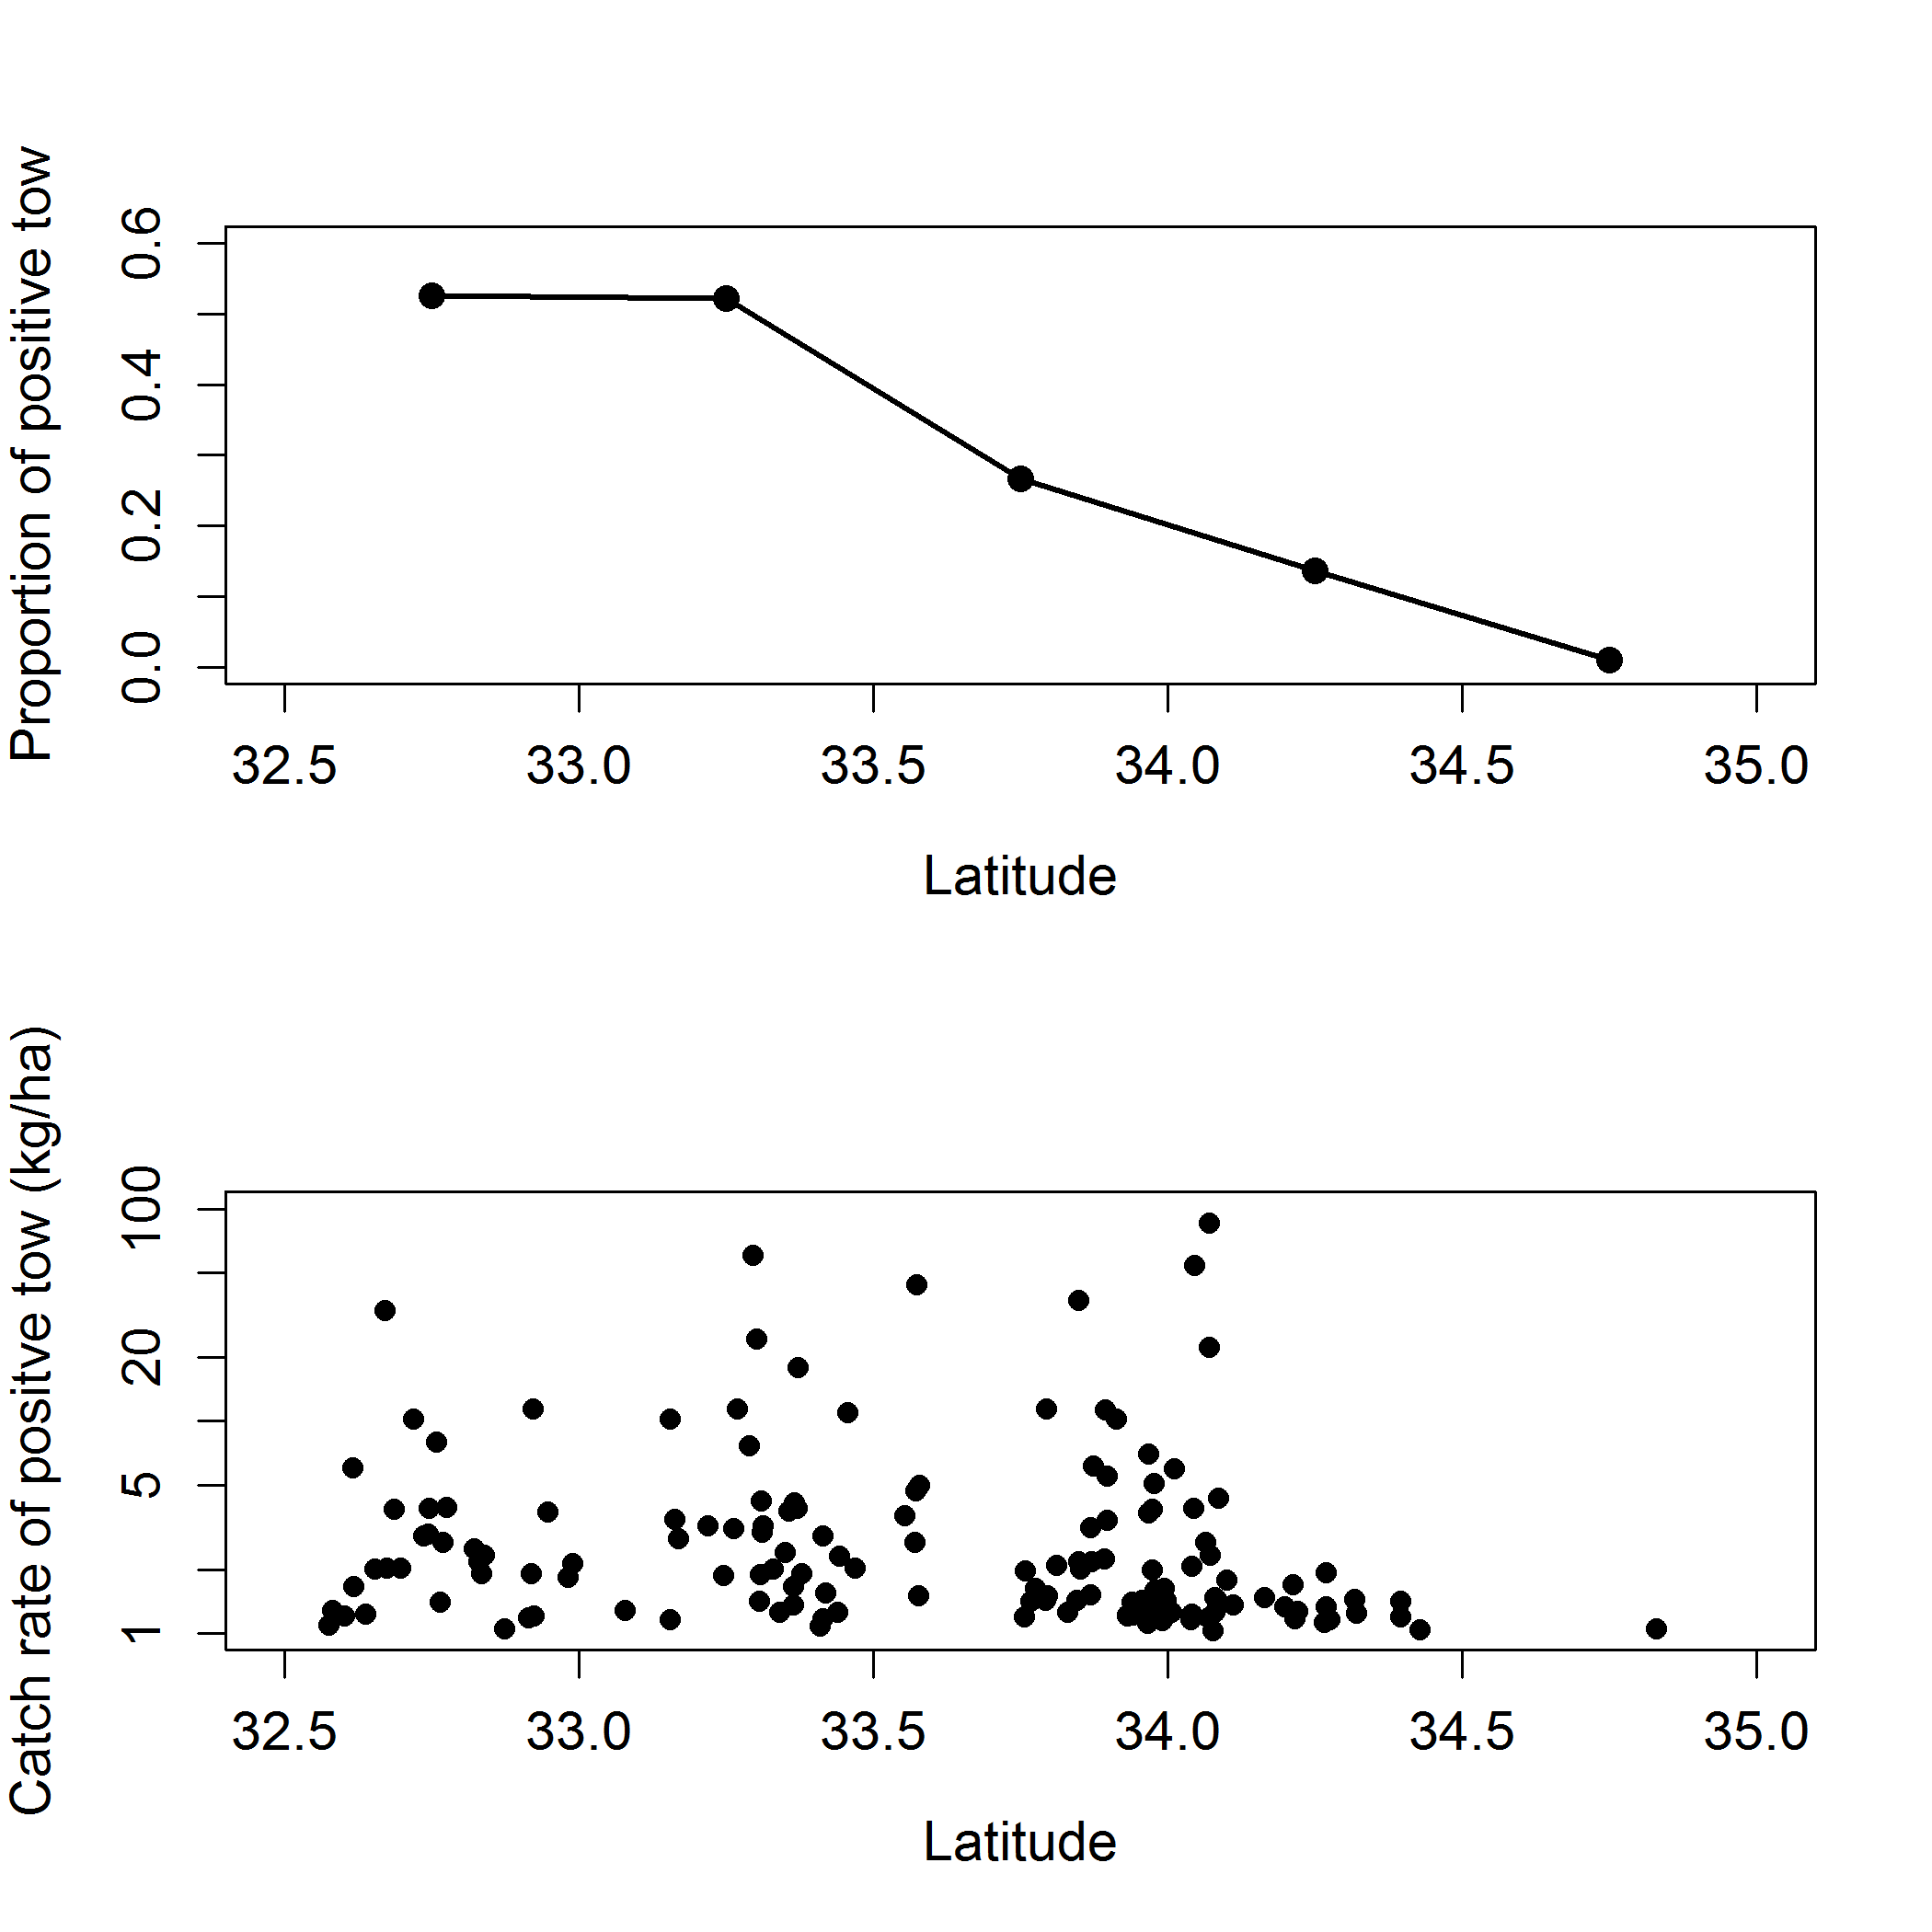
\includegraphics{Figures/NWFSCtrawl_poslat.png}
\caption{Plots of the proportion of positive tows (top panel) and the
raw catch rates of positive tows (bottom panel) by latitude zones (0.5
degree interval) for NWFSC trawl survey.
\label{fig:Fleet8_NWFSCtrawl_poslat}}
\end{figure}

\begin{figure}[htbp]
\centering
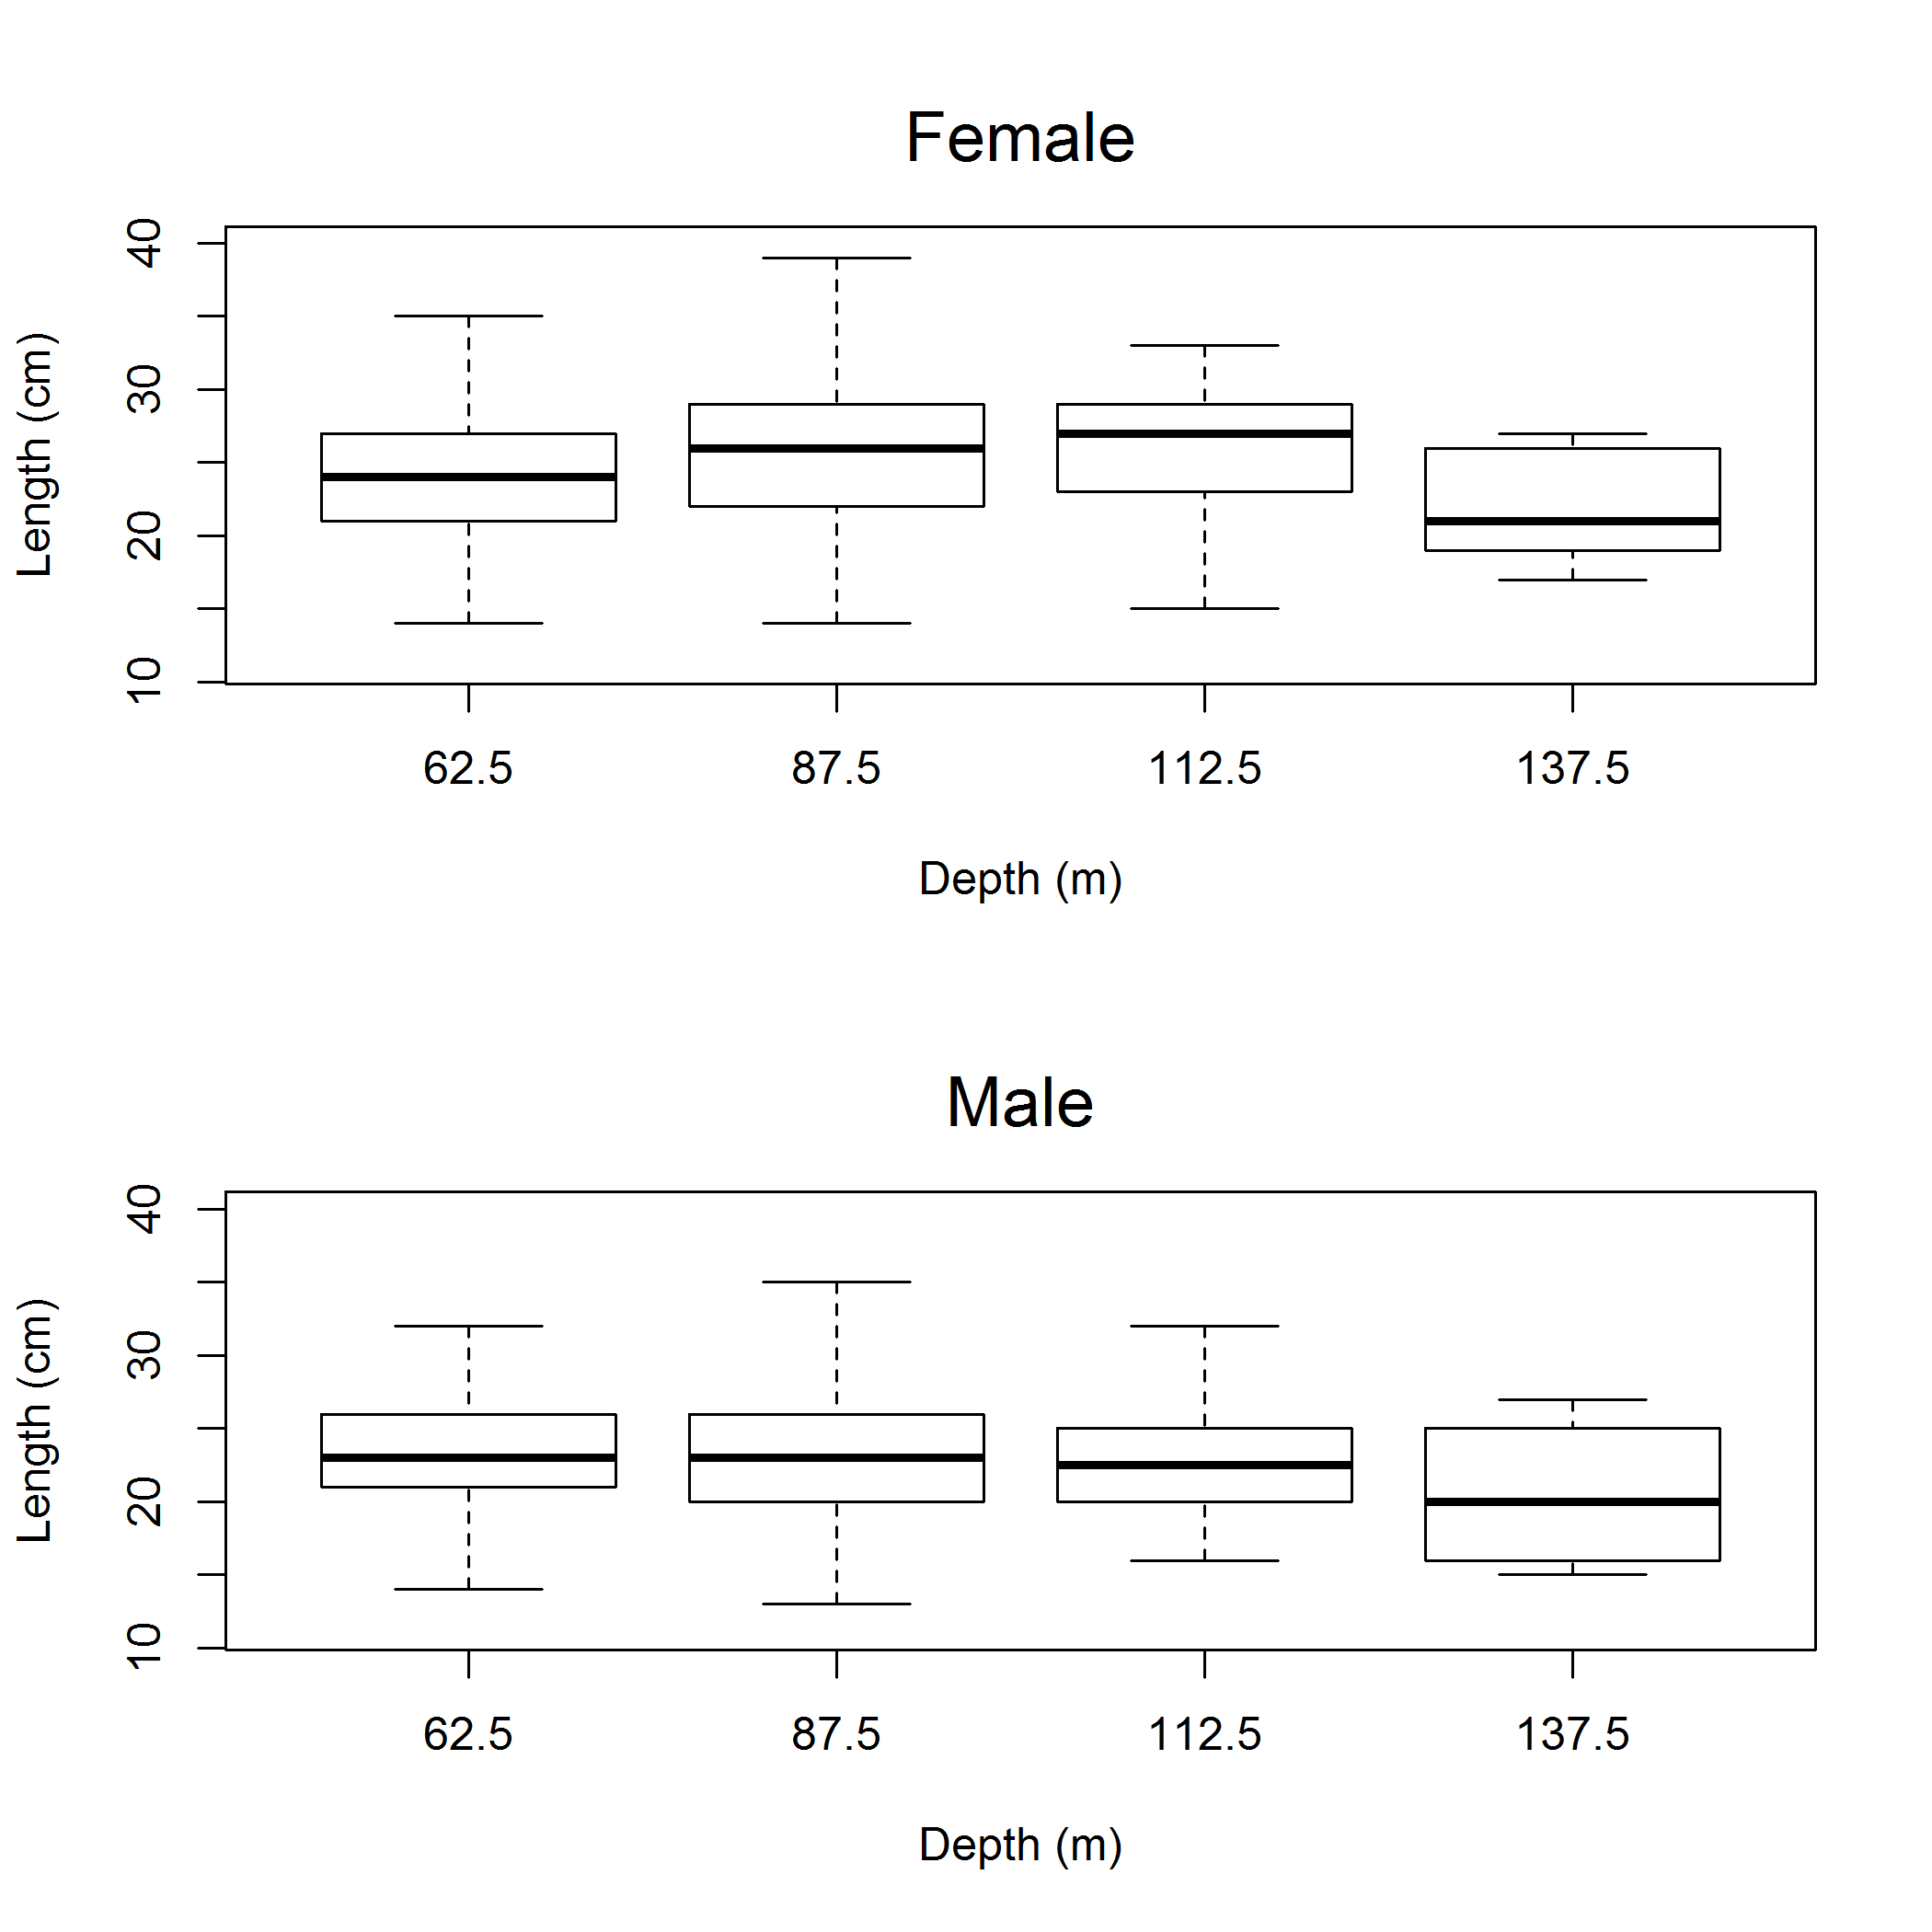
\includegraphics{Figures/NWFSCtrawl_lengthdepth.png}
\caption{Comparison box plots of raw length data from NWFSC trawl survey
by depth zone and sex. \label{fig:Fleet8_NWFSCtrawl_lengthdepth}}
\end{figure}

\begin{figure}[htbp]
\centering
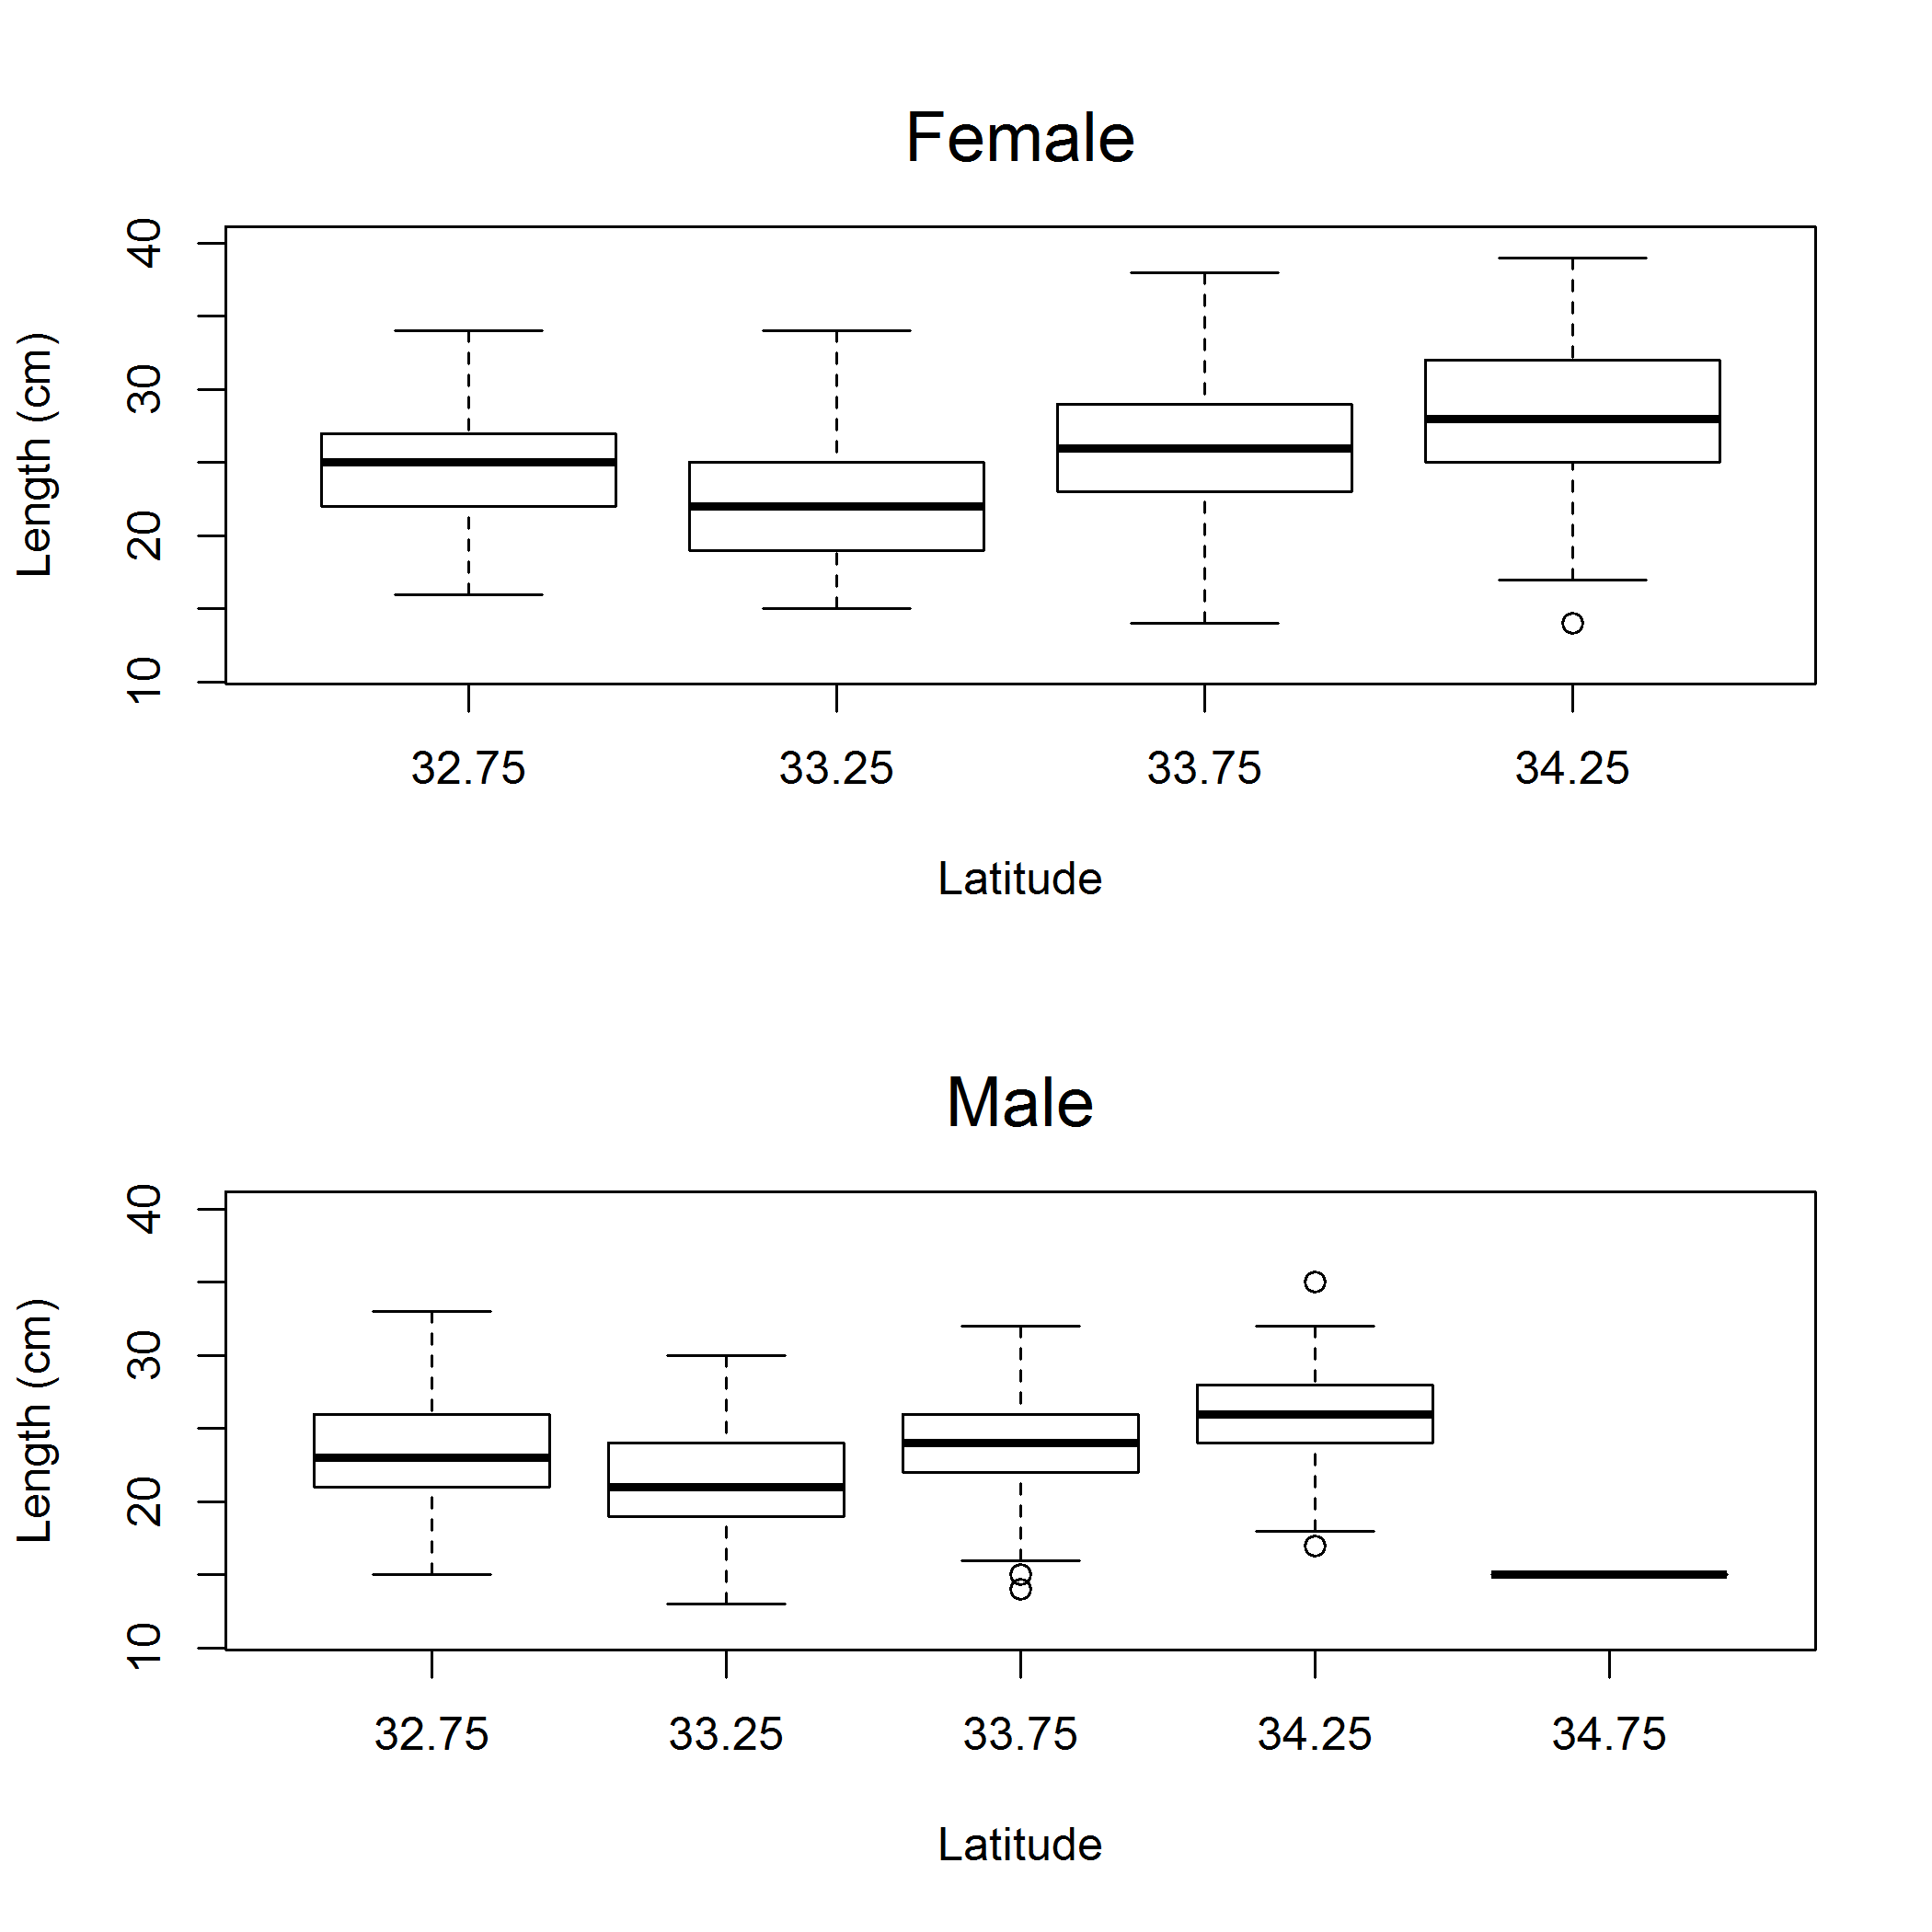
\includegraphics{Figures/NWFSCtrawl_lengthlat.png}
\caption{Comparison box plots of raw length data from NWFSC trawl survey
by latitude zone and sex. \label{fig:Fleet8_NWFSCtrawl_lengthlat}}
\end{figure}

\begin{figure}[htbp]
\centering
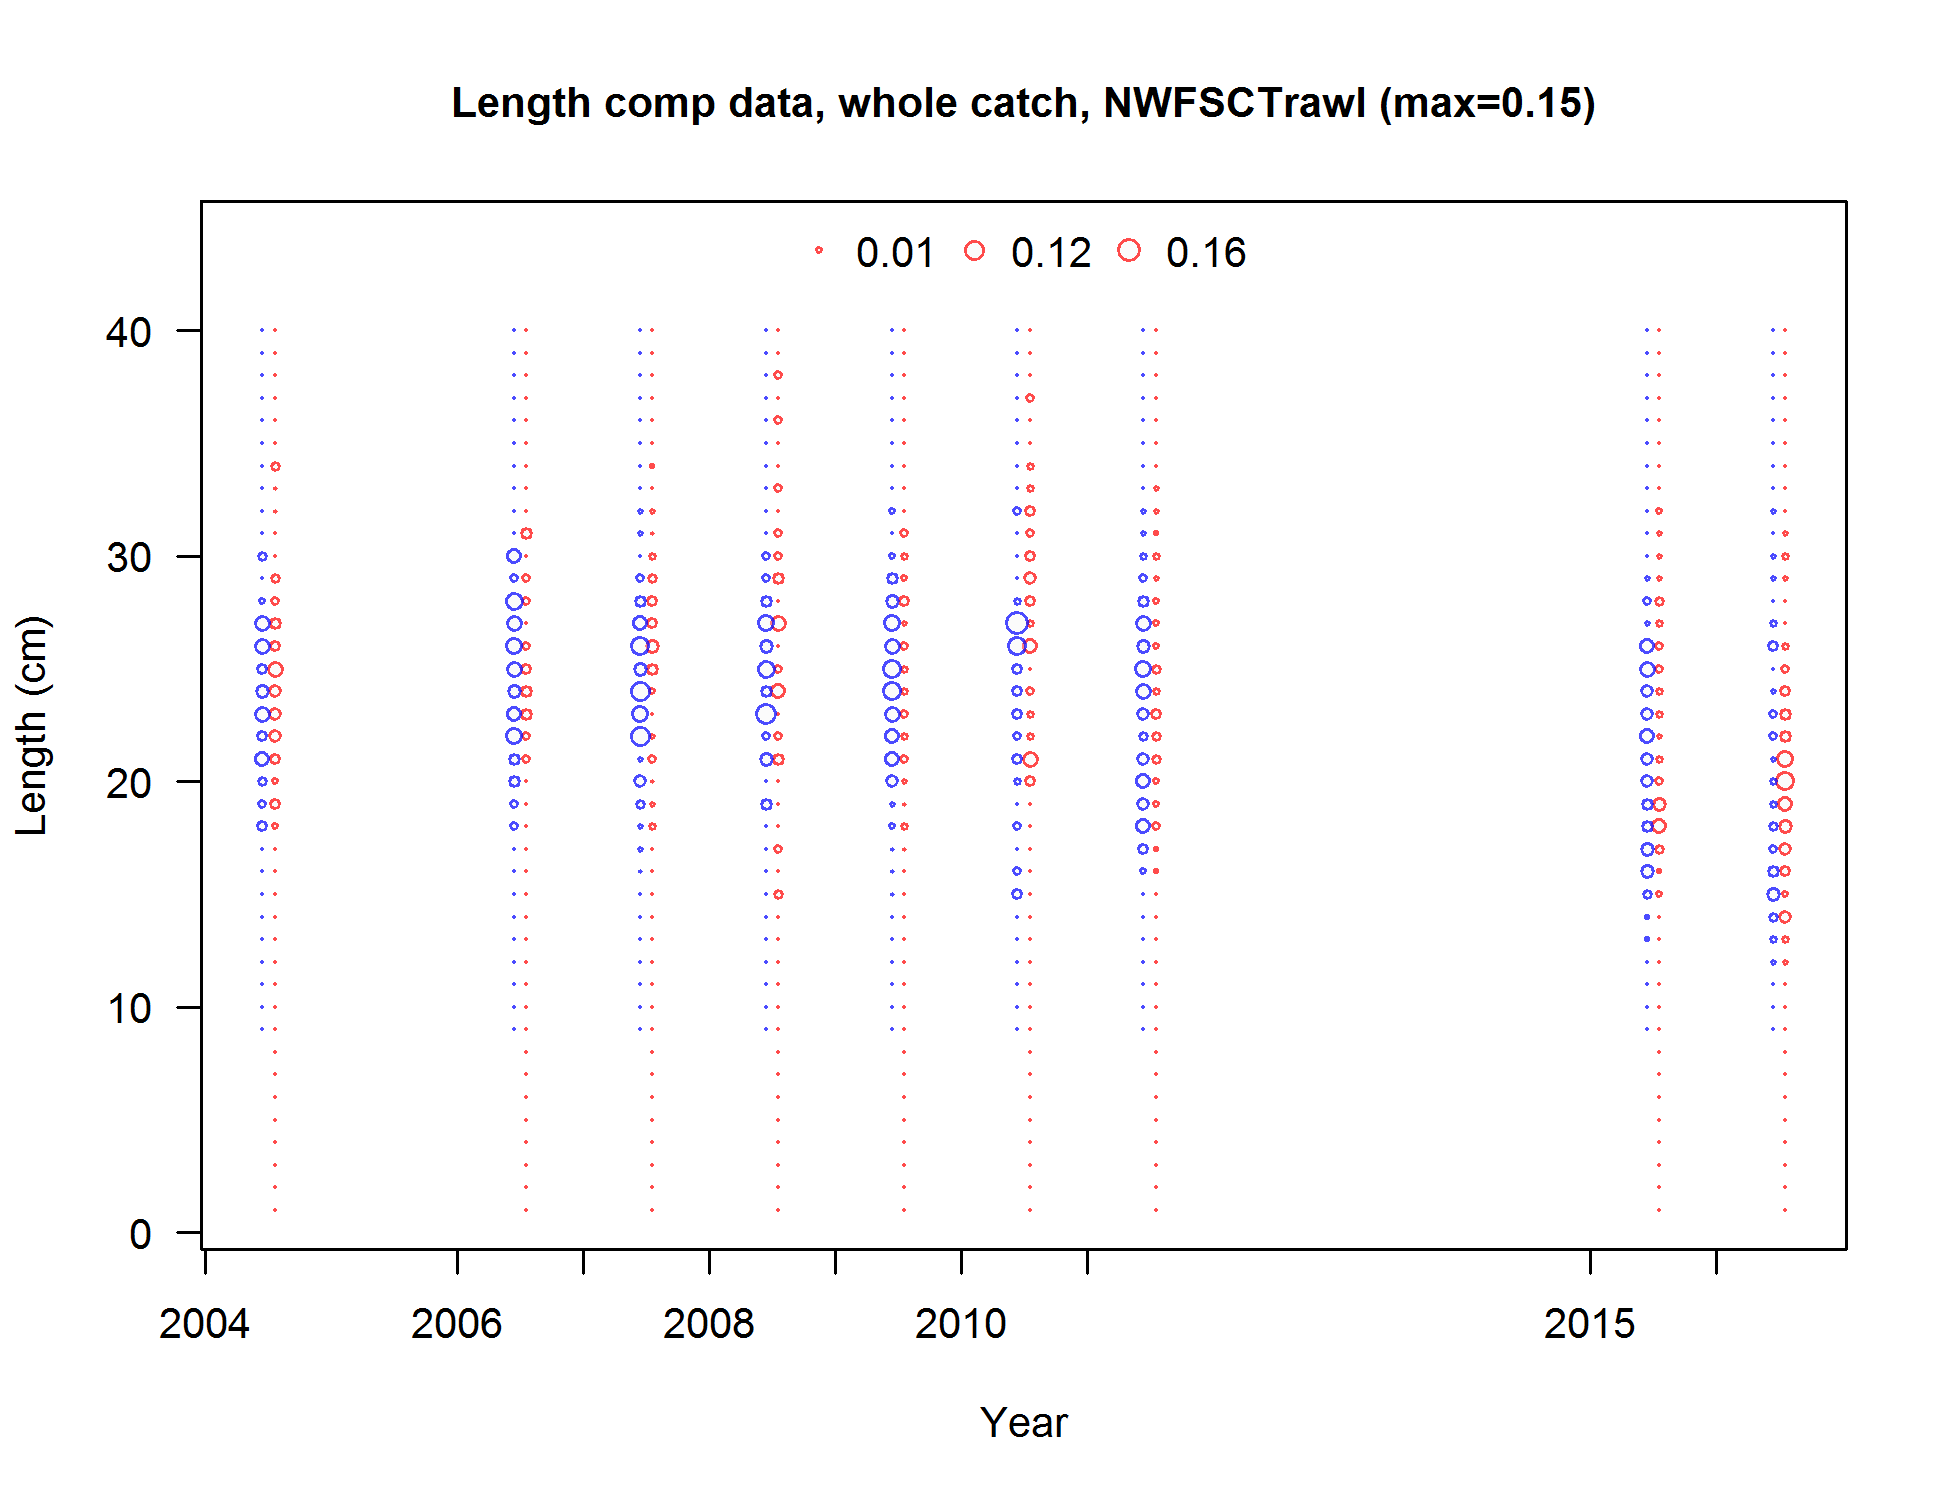
\includegraphics{r4ss/plots_mod1/comp_lendat_bubflt8mkt0.png}
\caption{Length frequency distributions of females (red) and male (blue)
from the NWFSC trawl survey between 2003 and 2016.
\label{fig:Fleet8_comp_lendat_bubflt8mkt0}}
\end{figure}

\begin{figure}[htbp]
\centering
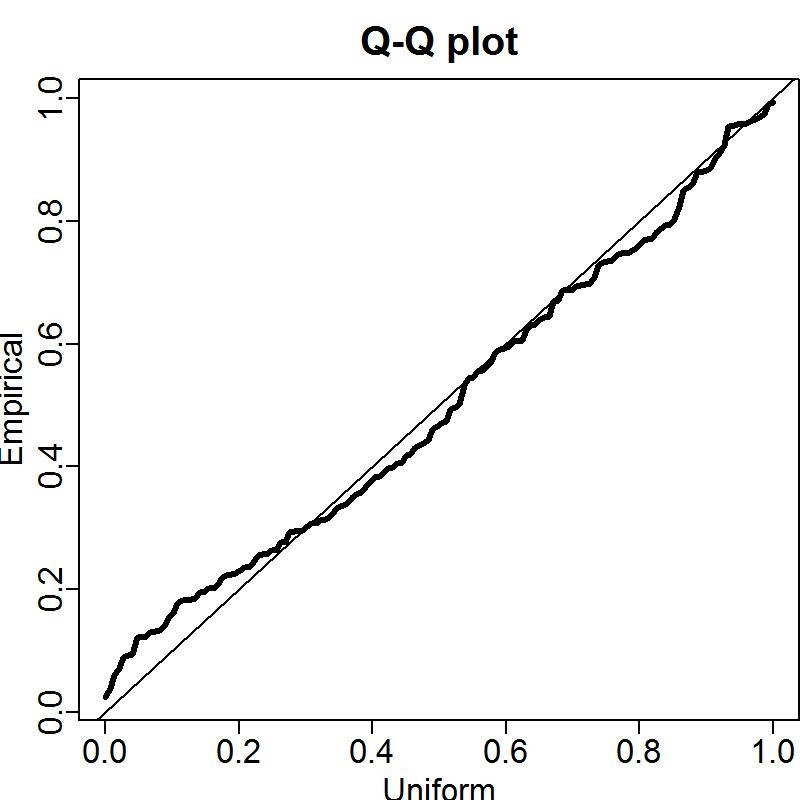
\includegraphics{Figures/NWFSCtrawl_QQ.jpg}
\caption{Q-Q plot used to validate the goodness of fit of the VAST
analysis for the NWFSC trawl survey between 2003 and 2016.
\label{fig:Fleet8_NWFSCtrawl_QQ}}
\end{figure}

\begin{figure}[htbp]
\centering
\includegraphics{r4ss/plots_mod1/index5_logcpuefit_NWFSCtrawl.png}
\caption{Fit to log index data on log scale for the NWFSC trawl survey
from the VAST analysis from 2003-2016. Lines indicate 95\% uncertainty
interval around index values. Thicker lines indicate input uncertainty
before addition of estimated additional uncertainty parameter.
\label{fig:index5_logcpuefit_NWFSCtrawl}}
\end{figure}

\FloatBarrier

\begin{figure}[htbp]
\centering
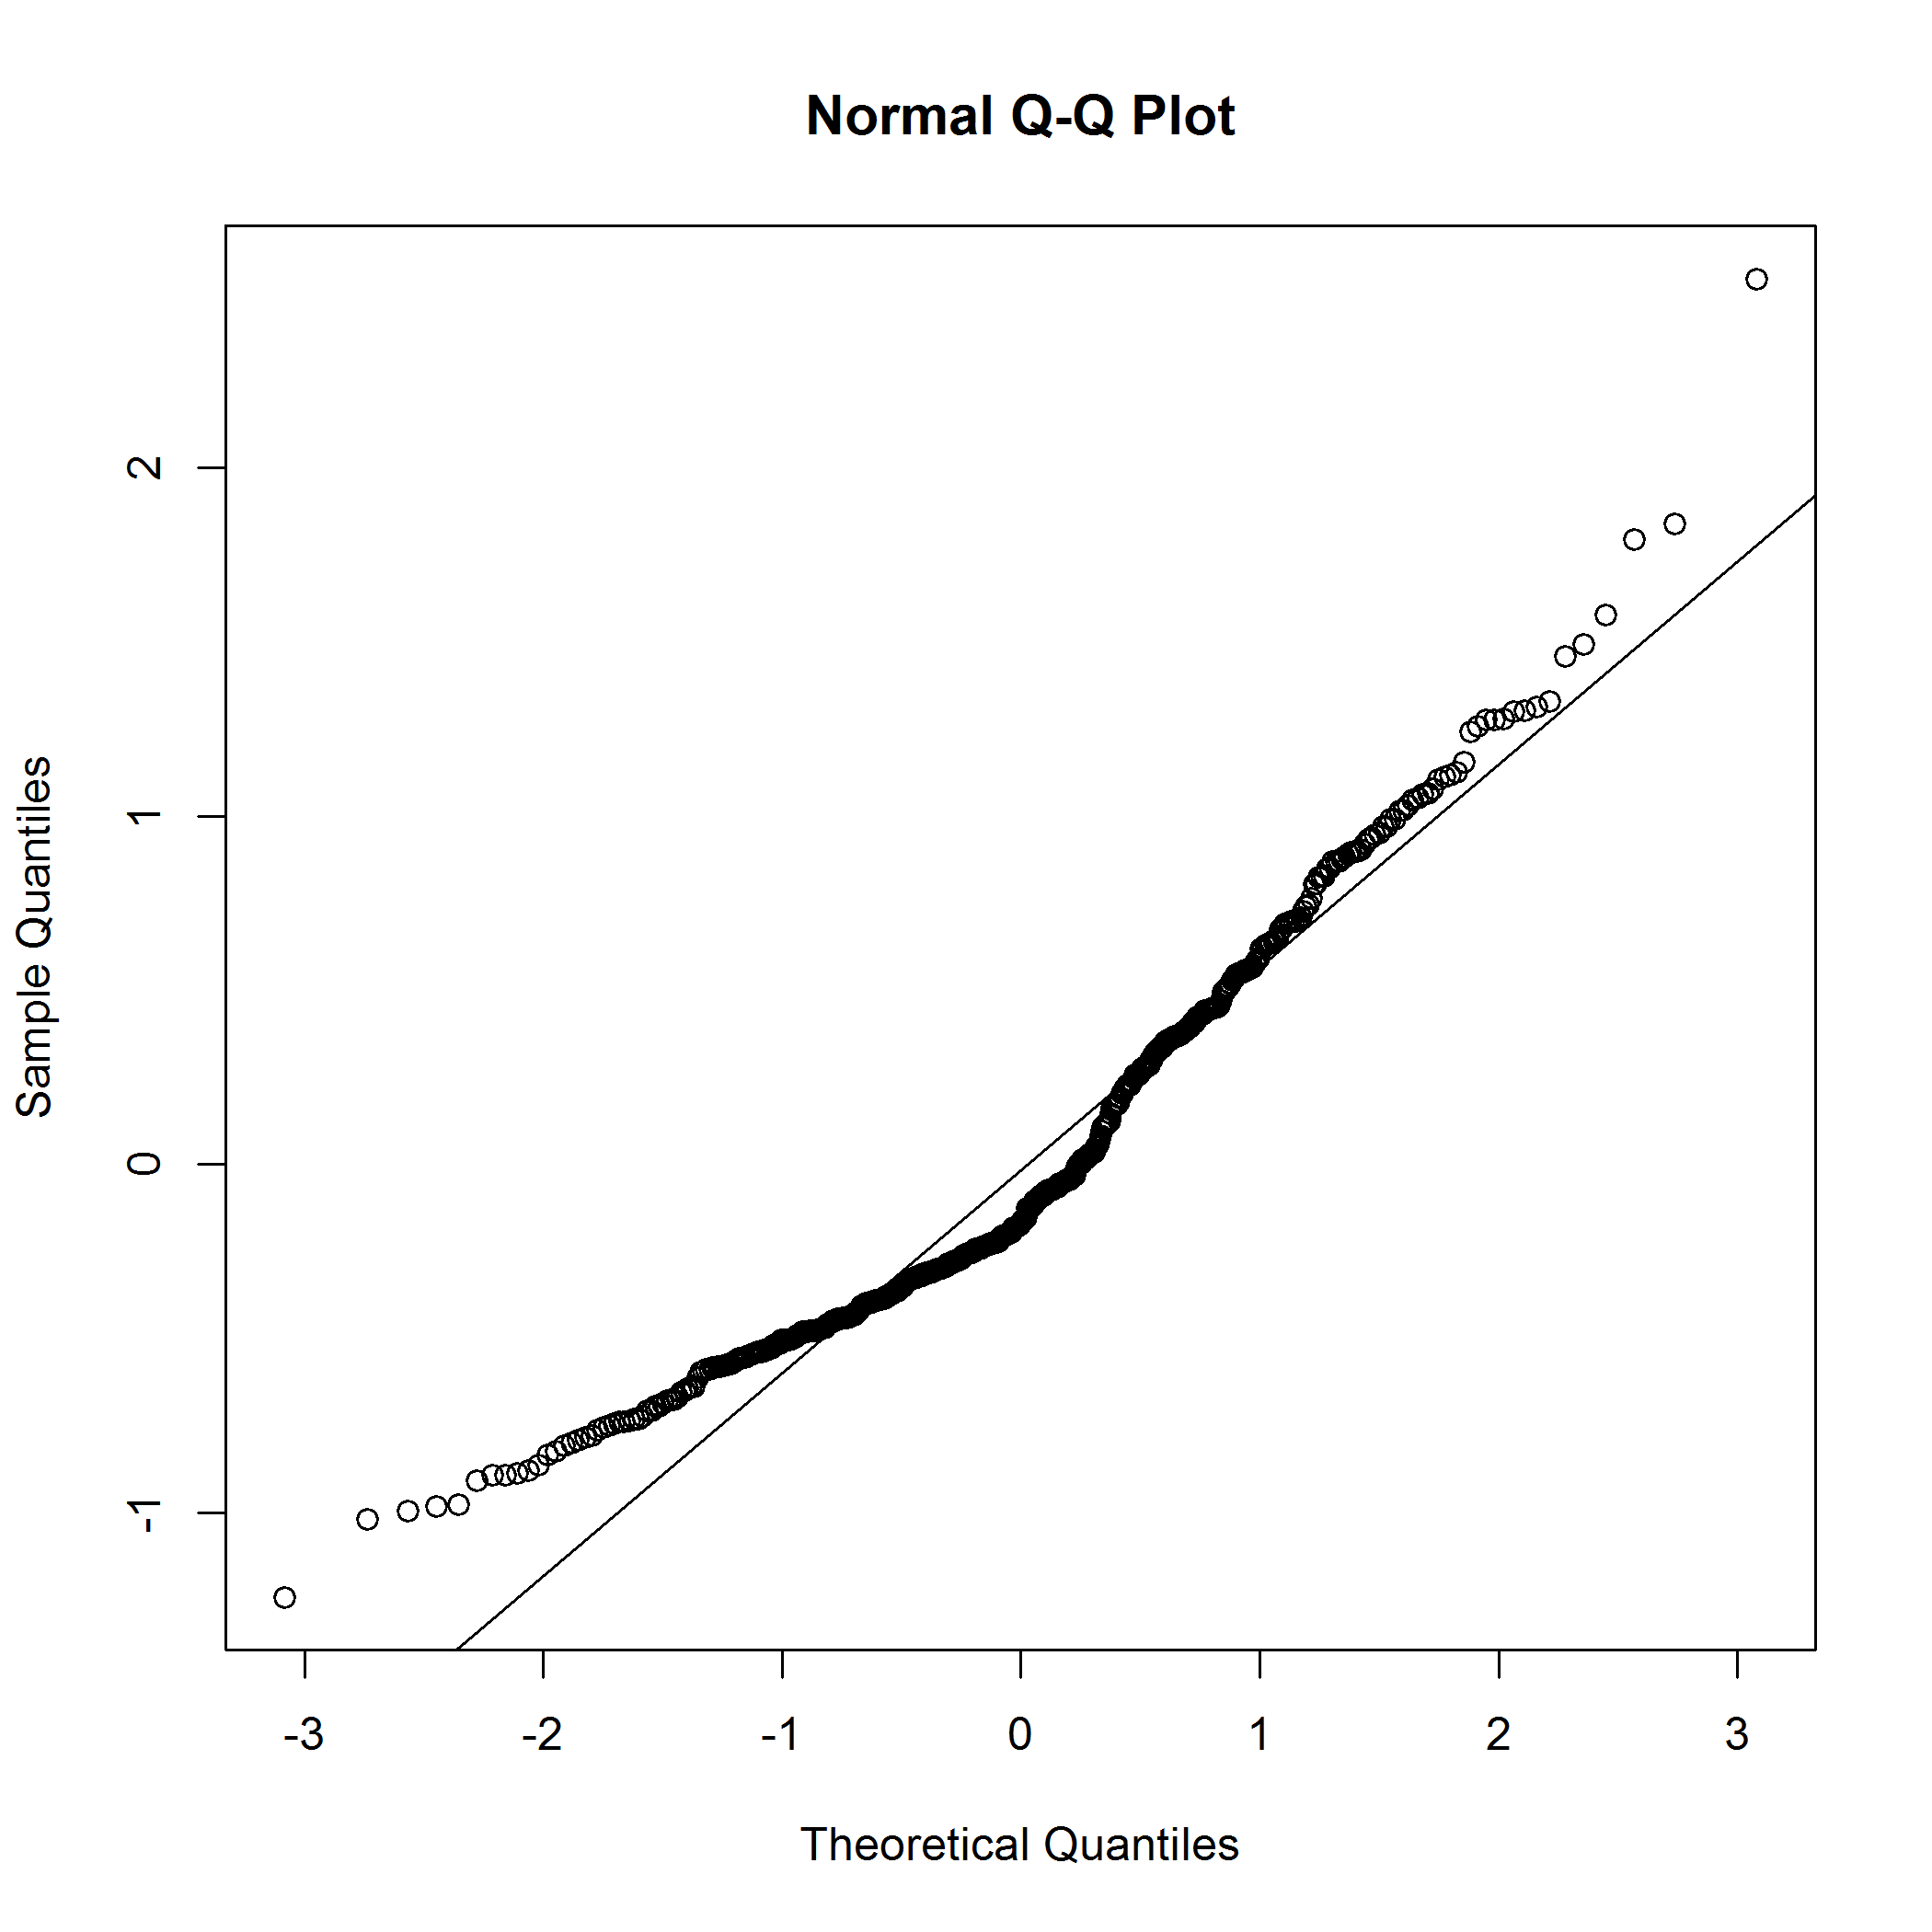
\includegraphics{Figures/Fleet9_GillnetSurvey_QQ.png}
\caption{Q-Q plot used to validate the goodness of fit of the lognormal
model for the CSUN/VRG gillnet survey from 1995-2008.
\label{fig:Fleet9_GillnetSurvey_QQ}}
\end{figure}

\begin{figure}[htbp]
\centering
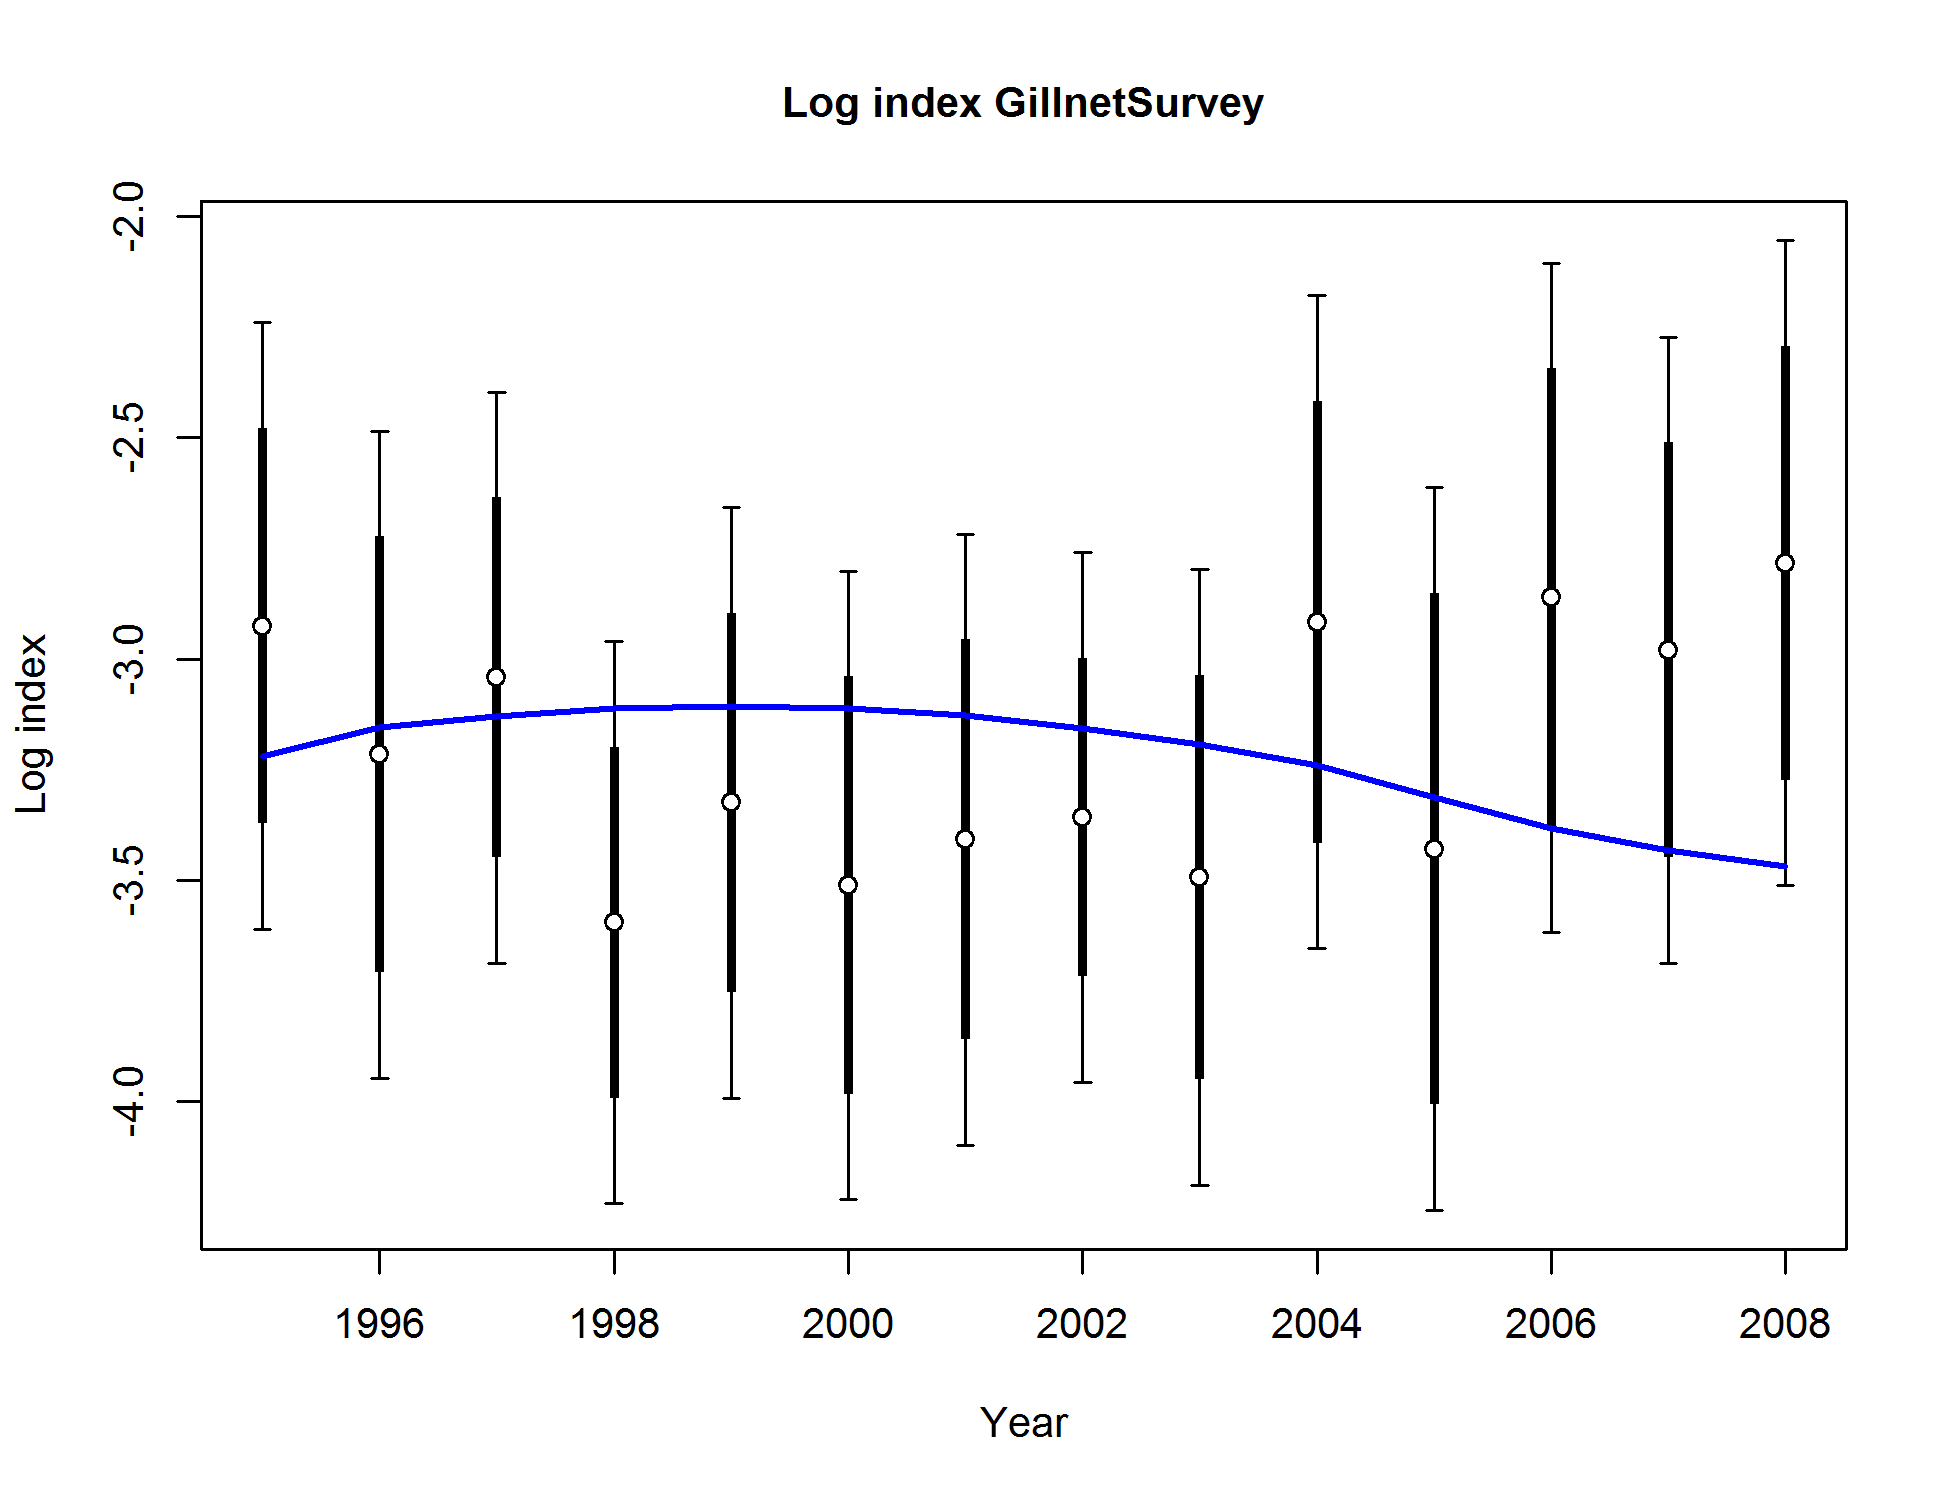
\includegraphics{r4ss/plots_mod1/index5_logcpuefit_GillnetSurvey.png}
\caption{Fit to log index data on log scale for the recreational
CSUN/VRG gillnet survey. Lines indicate 95\% uncertainty interval around
index values. Thicker lines indicate input uncertainty before addition
of estimated additional uncertainty parameter.
\label{fig:index5_logcpuefit_GillnetSurvey}}
\end{figure}

\FloatBarrier

\begin{figure}[htbp]
\centering
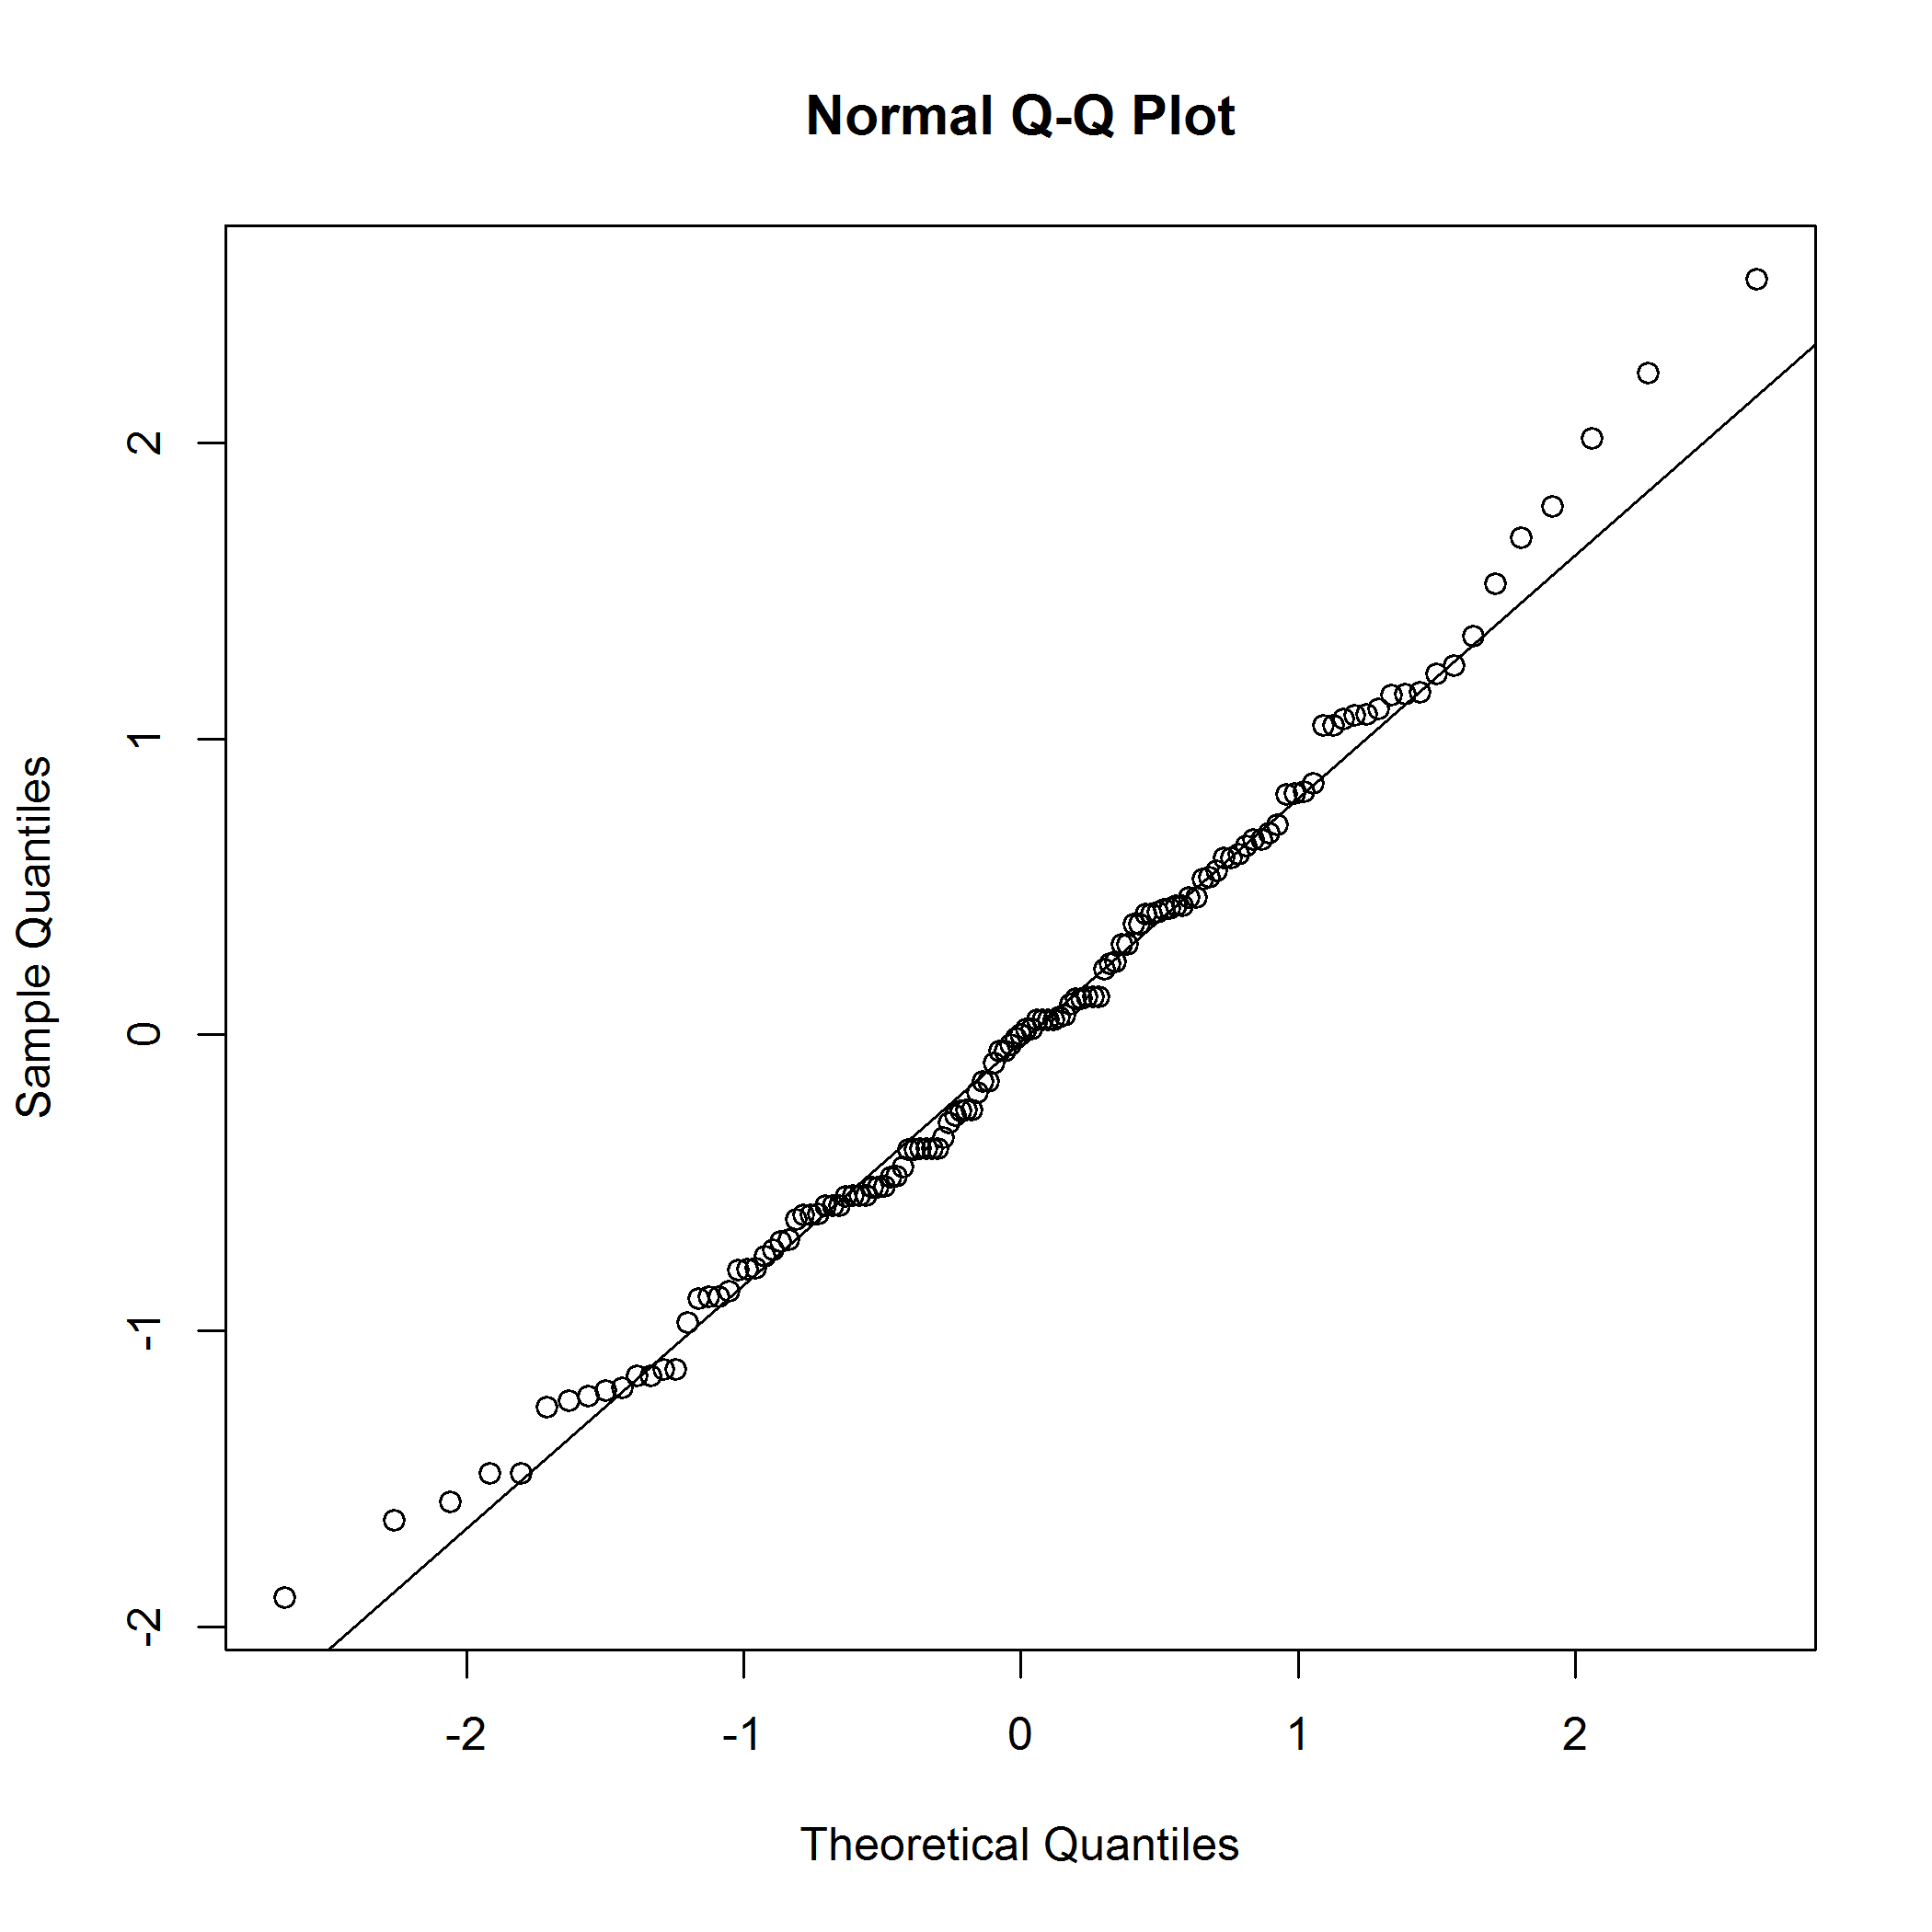
\includegraphics{Figures/Fleet11_SCBsurvey_QQ.png}
\caption{Q-Q plot used to validate the goodness of fit of the lognormal
model for the Southern California Bight monitoring program trawl survey.
\label{fig:Fleet11_SCBsurvey_QQ}}
\end{figure}

\begin{figure}[htbp]
\centering
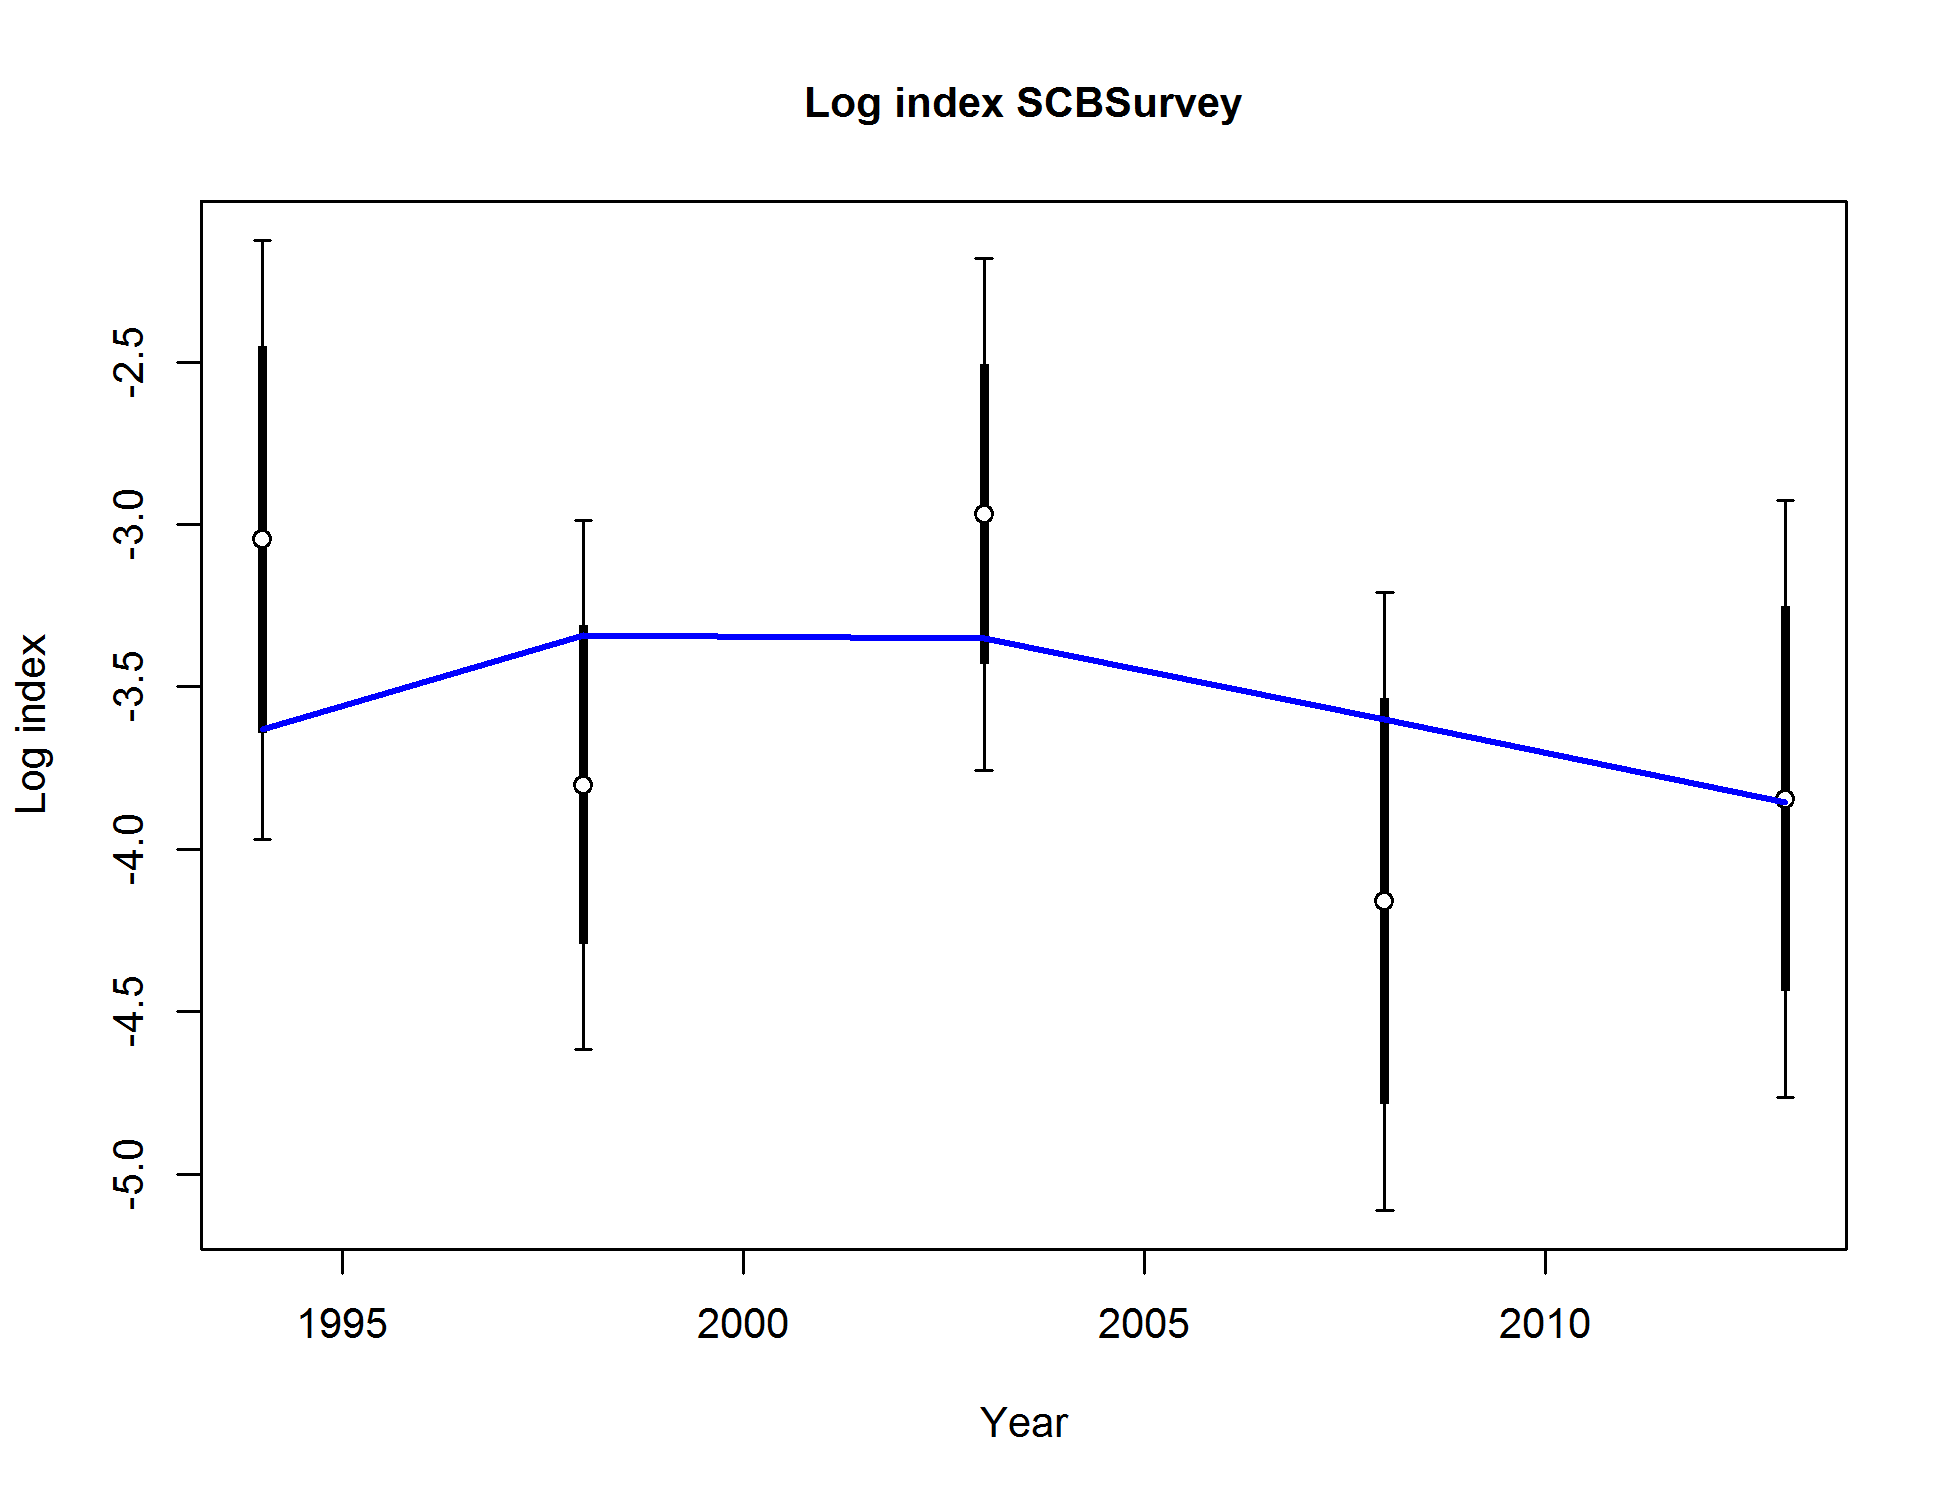
\includegraphics{r4ss/plots_mod1/index5_logcpuefit_SCBSurvey.png}
\caption{Fit to log index data on log scale for the recreational
Southern California Bight trawl survey. Lines indicate 95\% uncertainty
interval around index values. Thicker lines indicate input uncertainty
before addition of estimated additional uncertainty parameter.
\label{fig:index5_logcpuefit_SCBSurvey}}
\end{figure}

\begin{figure}[htbp]
\centering
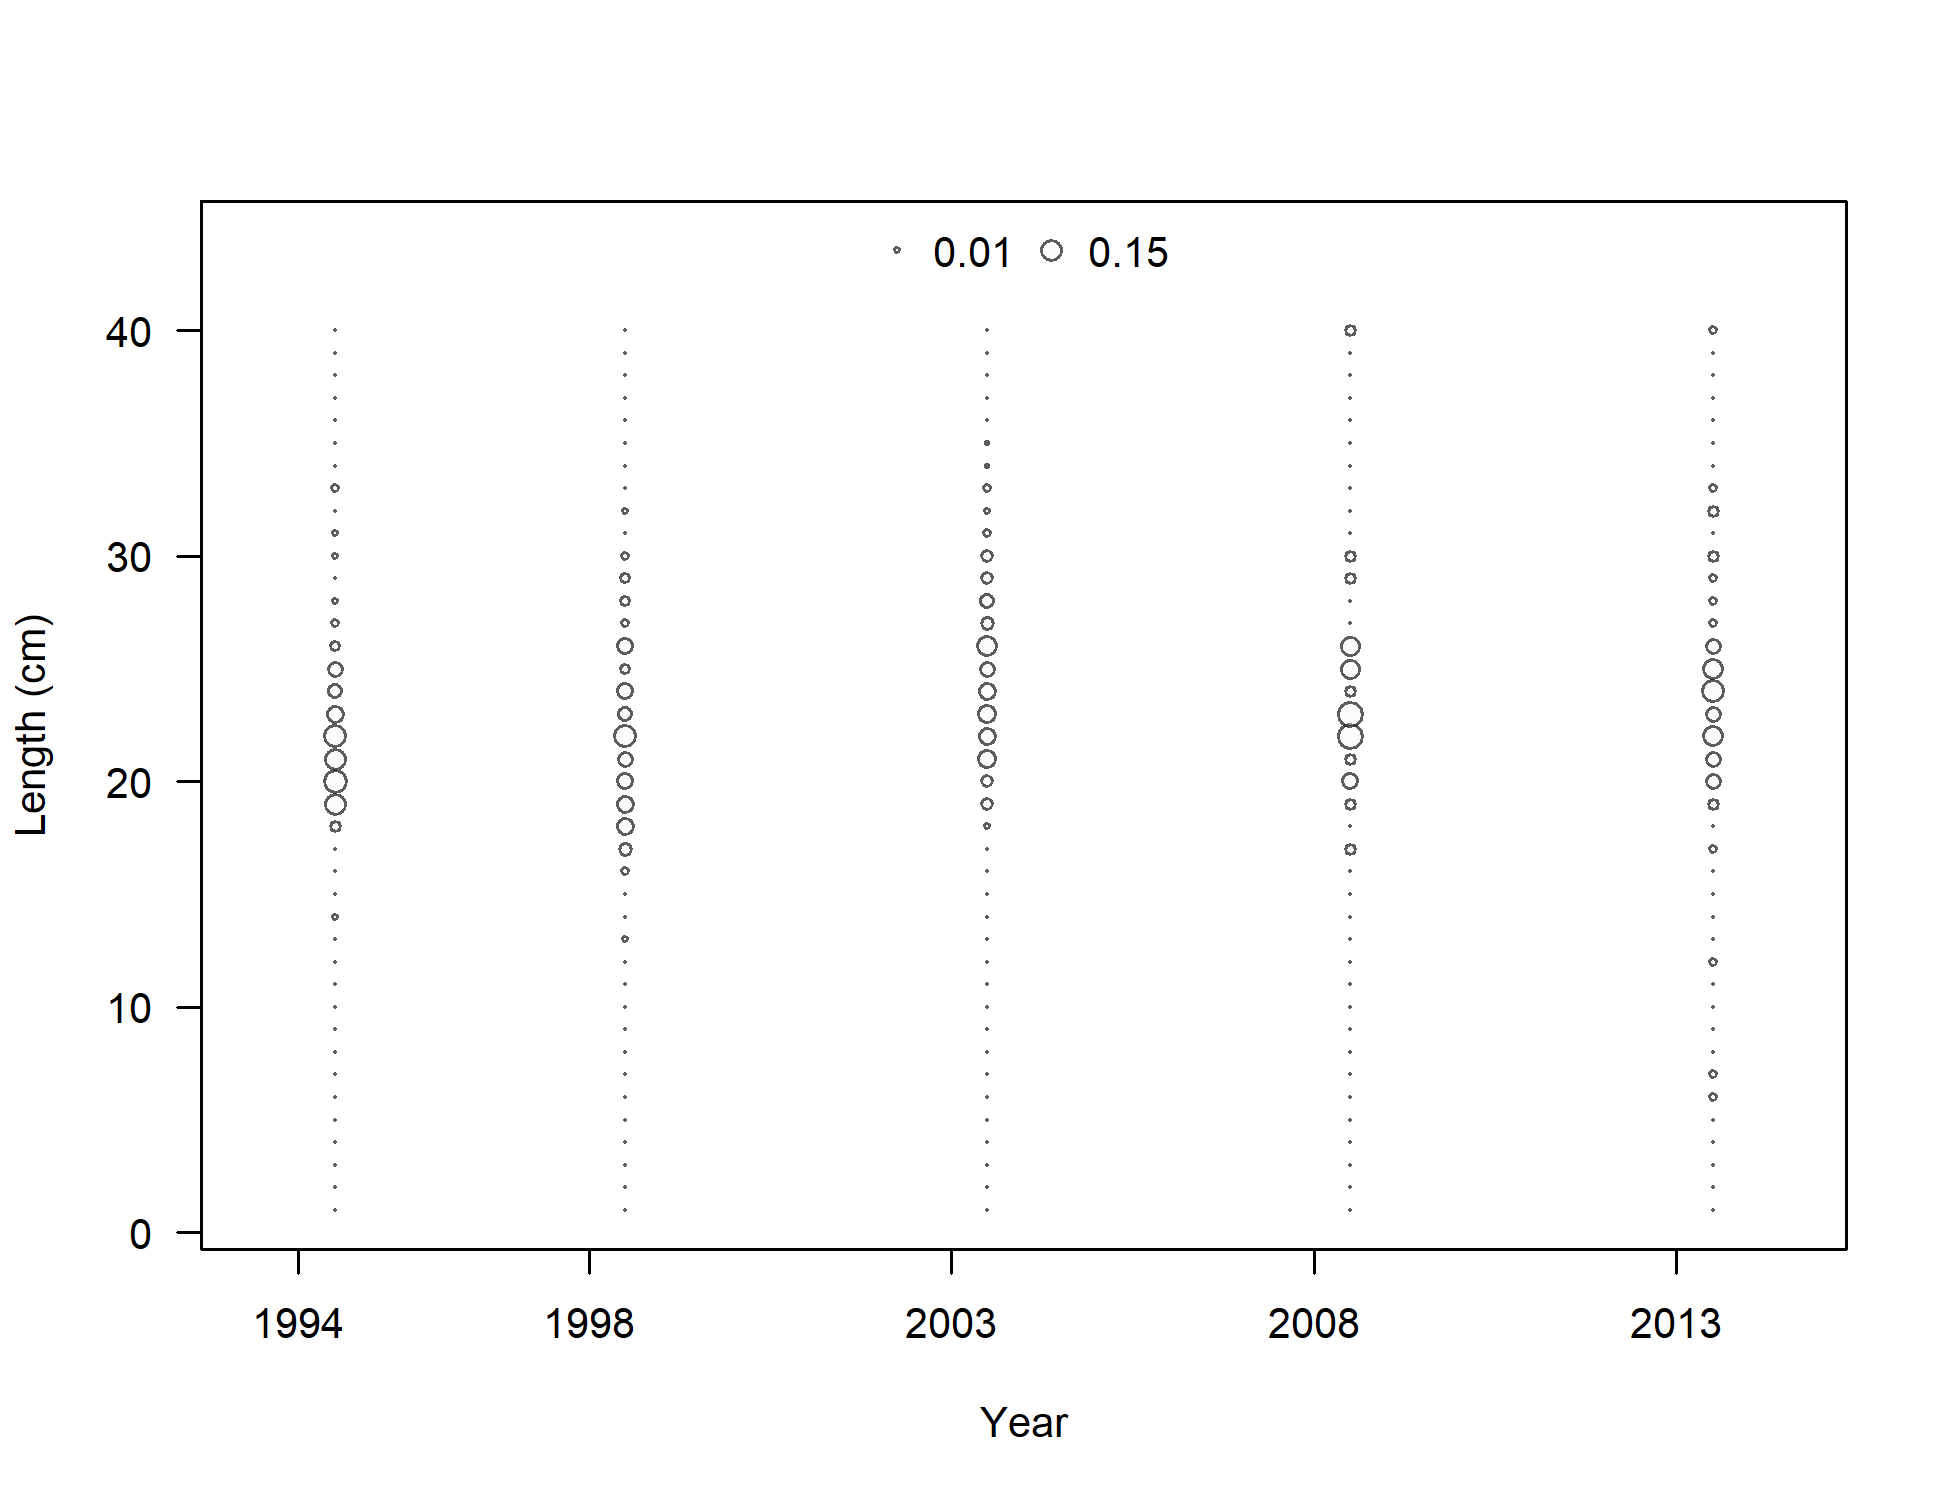
\includegraphics{r4ss/plots_mod1/comp_lendat_bubflt11mkt2.png}
\caption{Length frequency distributions from the Southern California
Bight regional monitoring program trawl surveys.
\label{fig:Fleet11_SCBsurvey_lendat_bubflt11mkt2}}
\end{figure}

\begin{figure}[htbp]
\centering
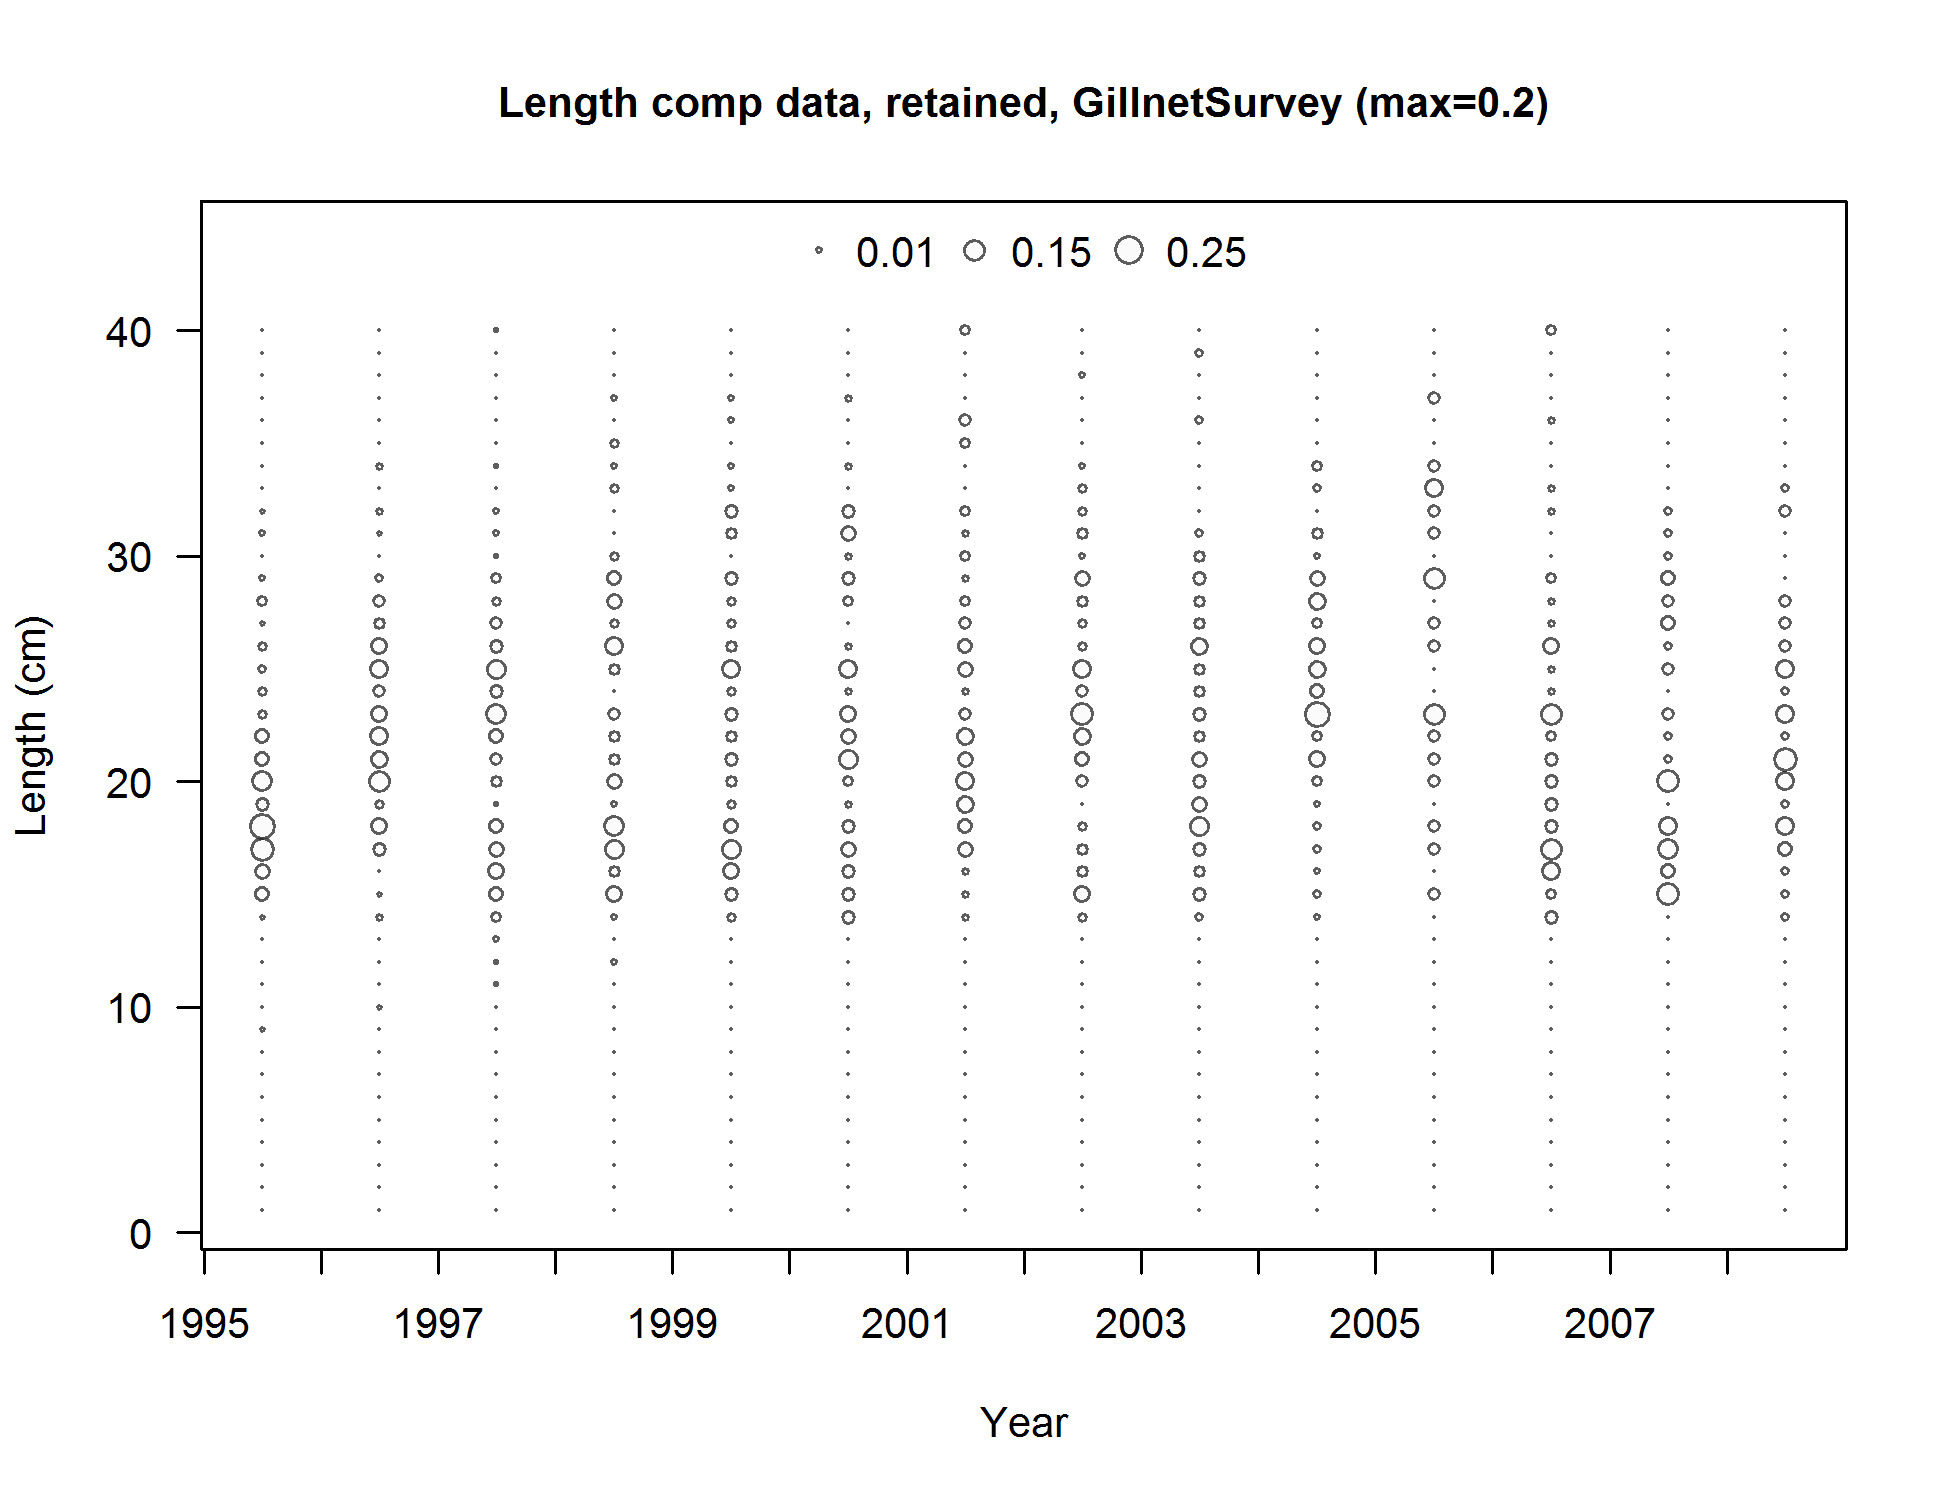
\includegraphics{r4ss/plots_mod1/comp_lendat_bubflt9mkt2.png}
\caption{Length frequency distributions from the Impingement surveys.
\label{fig:Fleet9_GillnetSurvey_lendat_bubflt10mkt2}}
\end{figure}

\begin{figure}[htbp]
\centering
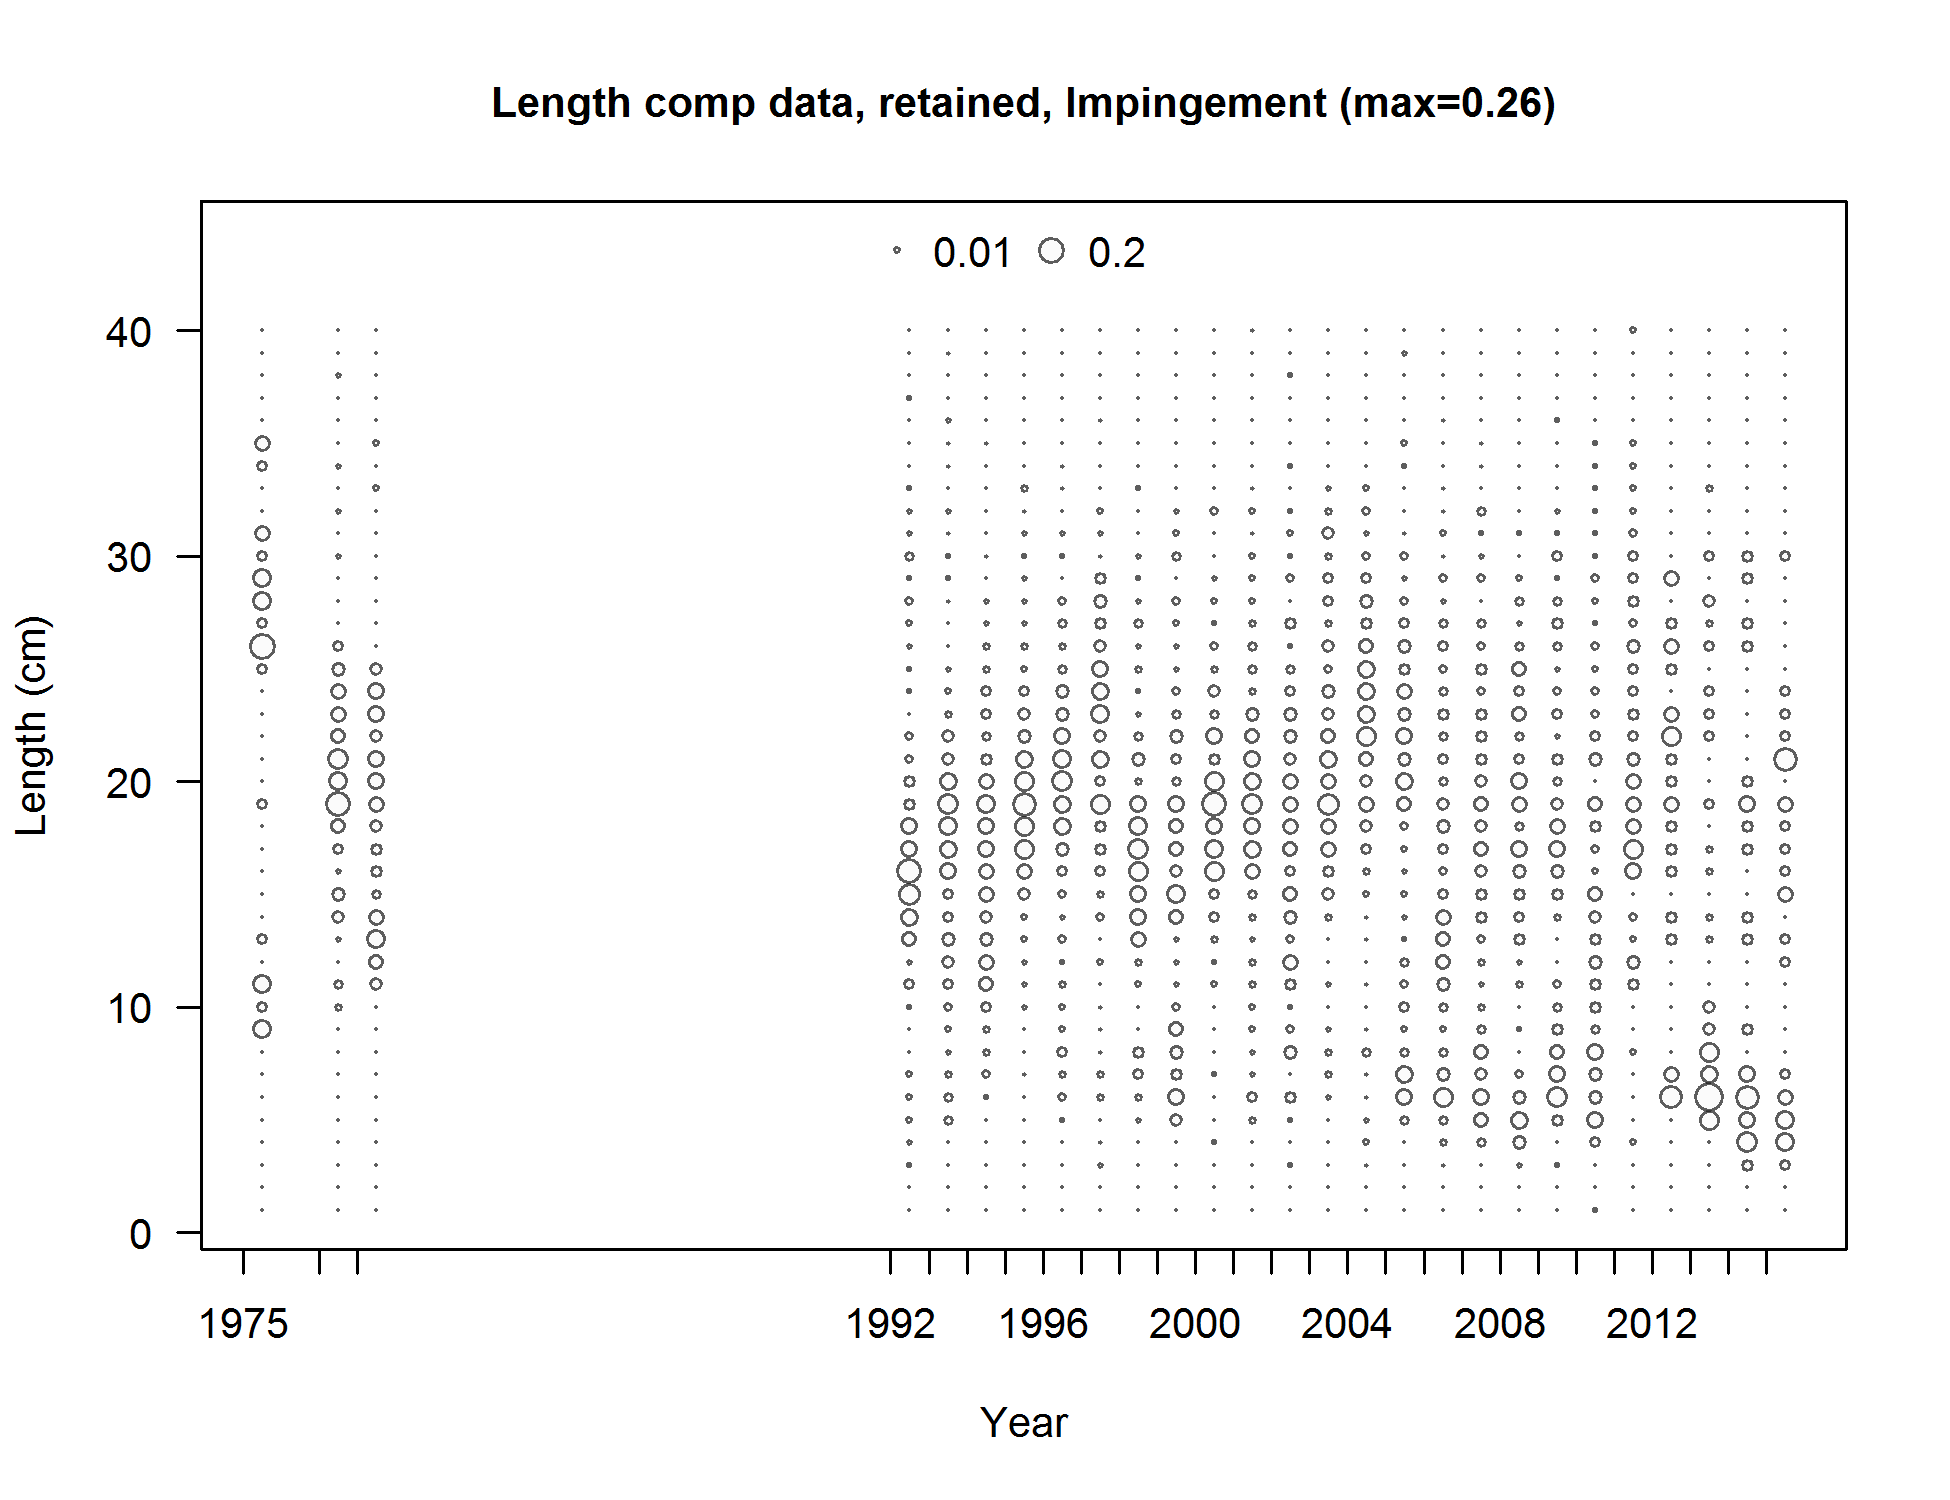
\includegraphics{r4ss/plots_mod1/comp_lendat_bubflt10mkt2.png}
\caption{Length frequency distributions from the Impingement surveys.
\label{fig:Fleet10_comp_lendat_bubflt10mkt2}}
\end{figure}

\FloatBarrier

\begin{figure}[htbp]
\centering
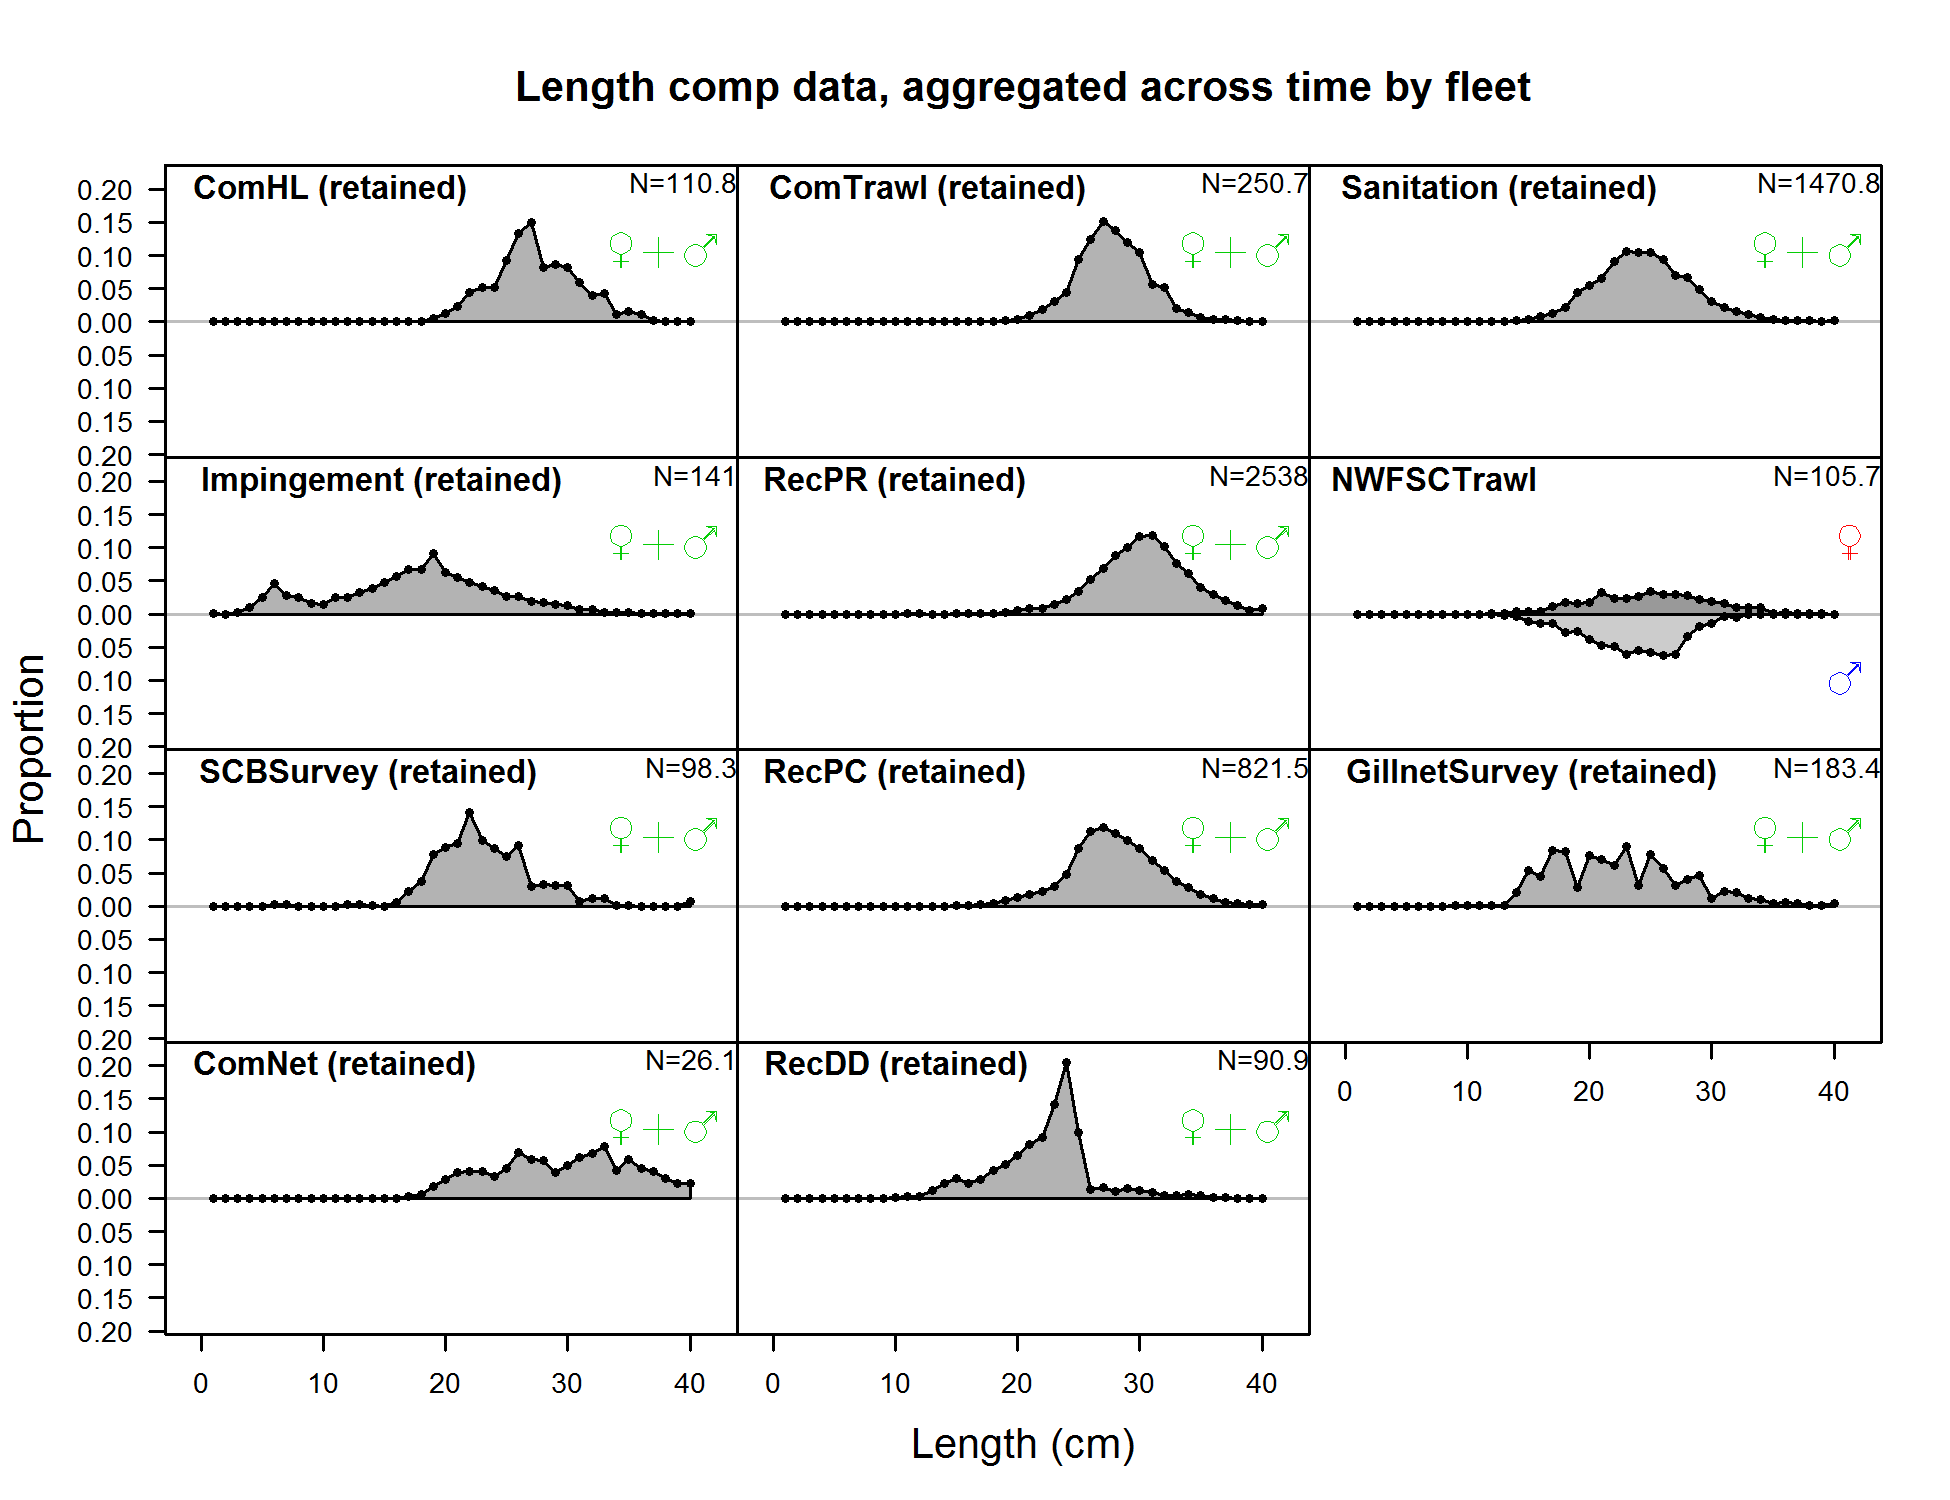
\includegraphics{r4ss/plots_mod1/comp_lendat__aggregated_across_time.png}
\caption{Length comp data, aggregated across time by fleet. Labels
`retained' and `discard' indicate discarded or retained sampled for each
fleet. Panels without this designation represent the whole catch.
\label{fig:comp_lendat_aggregated_across_time}}
\end{figure}

\FloatBarrier

\begin{figure}[htbp]
\centering
\includegraphics{Figures/otolith1.pdf}
\caption{Cross-section of broken and burned California scorpionfish
otolith showing. The green dots indicate the number of increments (photo
courtesy Lance Sullivan, NWFSC). \label{fig:otolith1}}
\end{figure}

\begin{figure}[htbp]
\centering
\includegraphics{Figures/otolith2.pdf}
\caption{California scorpionfish otolith (photo courtesy Lance Sullivan,
NWFSC). \label{fig:otolith2}}
\end{figure}

\begin{figure}[htbp]
\centering
\includegraphics{Figures/Age_length_bySex.png}
\caption{Length at age by sex for California scorpionfish collected from
the NWFSC trawl survey. \label{fig:Agelength}}
\end{figure}

\begin{figure}[htbp]
\centering
\includegraphics{Figures/vonB_compare.png}
\caption{Fitted (external to SS) von Bertalanffy growth by sex for
California scorpionfish collected from the NWFSC trawl survey.
\label{fig:vonB_compare}}
\end{figure}

\begin{figure}[htbp]
\centering
\includegraphics{Figures/Fleet8_NWFSCTrawl_ageerror.png}
\caption{Aging precision between two current age readers at the NWFSC.
\label{fig:Fleet8_NWFSCTrawl_ageerror}}
\end{figure}

\begin{figure}[htbp]
\centering
\includegraphics{Figures/Fleet8_NWFSCTrawl_ageerror2.pdf}
\caption{True versus predicted age for two current age readers at the
NWFSC from the ageing error software with unbiased reads and curivlinear
standard deviation for both readers.
\label{fig:Fleet8_NWFSCTrawl_ageerror2}}
\end{figure}

\begin{figure}[htbp]
\centering
\includegraphics{Figures/Length_weight.png}
\caption{Comparison of the California scorpionfish weight-length curves
from Love et al. (1987) and those estimated from the NWFSC trawl survey.
\label{fig:Length_weight}}
\end{figure}

\newpage

\color{black}

\section*{References}\label{references}
\addcontentsline{toc}{section}{References}

\renewcommand{\thepage}{}

\hypertarget{refs}{}
\hypertarget{ref-Ally1991}{}
Ally, J., Ono, D., Read, R.B., and Wallace, M. 1991. Status of major
southern California marine sport fish species with management
recommendations, based on analyses of catch and size composition data
colleced on board commercial passenger fishing vessels from 1985 through
1987. Marine Resouces Division Administrative Report No. 90-2.

\hypertarget{ref-Alverson1964}{}
Alverson, D.L., Pruter, a T., and Ronholt, L.L. 1964. A Study of
Demersal Fishes and Fisheries of the Northeastern Pacific Ocean.
Institute of Fisheries, University of British Columbia.

\hypertarget{ref-vonB1938}{}
Bertalanffy, L. von. 1938. A quantitative theory of organic growth.
Human Biology \textbf{10}: 181--213.

\hypertarget{ref-Bight1998}{}
Bight '98 Steering Committee. 1998. Field Operations Manual. Commission
of Southern California Coastal Water Research Project, Westminster, CA.

\hypertarget{ref-Collins1978}{}
Collins, R., and Crooke, S. (n.d.). An evaluation of the commercial
passenger fishing vesselrecord system and the results of sampling the
Southern California catch for species and size composition, 1975-1978.
Unpublished report.

\hypertarget{ref-Daugherty1949}{}
Daugherty, A. 1949. The commercial fish catch of California for the year
1947 With an historical review 1916--1947. \emph{In} California
department of fish and game fishery bulletin no. 74.

\hypertarget{ref-Dotson2003}{}
Dotson, R., and Charter, R. 2003. Trends in the Southern California
sport fishery. CalCOFI Report \textbf{44}: 94--106. Available from
\url{http://calcofi.org/publications/calcofireports/v44/Vol_44_Dotson_Charter.pdf}.

\hypertarget{ref-Eschmeyer1983}{}
Eschmeyer, W.N., Herald, E., and Hammann, H. 1983. A field guide to
Pacific coast fishes of North America. Houghton Mifflin Company, Boston,
MA.

\hypertarget{ref-Francis2011}{}
Francis, R. 2011. Data weighting in statistical fisheries stock
assessment models. Canadian Journal of Fisheries and Aquatic Sciencies
\textbf{68}: 1124--1138.

\hypertarget{ref-Frey1971}{}
Frey, H. 1971. California's living marine resources and their
utilization. California Department of Fish; Game, Sacramento, CA.

\hypertarget{ref-Hamel2015}{}
Hamel, O. 2015. A method for calculating a meta-analytical prior for the
natural mortality rate using multiple life history correlates. ICES
Journal of Marine Science \textbf{72}: 62--69.

\hypertarget{ref-Harry1961}{}
Harry, G., and Morgan, A. 1961. History of the trawl fishery, 1884-1961.
Oregon Fish Commission Research Briefs \textbf{19}: 5--26.

\hypertarget{ref-Hill1999}{}
Hill, K.T., and Schneider, N. 1999. Historical logbook databases from
California's commercial passenger fishing vessel (partyboat) fishery,
1936-1997. Scripps Institution of Oceanography References Series
\textbf{99-19}.

\hypertarget{ref-Jordan1887}{}
Jordan, D. 1887. The fisheries of the Pacific Coast. \emph{In} The
fisheries and fishery industris of the unistes states. \emph{Edited by}
G. Goode. U.S. Commision of Fish; Fisheries, Section 3. pp. 591--630.

\hypertarget{ref-Keller2008}{}
Keller, A.A., Horness, B.H., Fruh, E.L., Simon, V.H., Tuttle, V.J.,
Bosley, K.L., Buchanan, J.C., Kamikawa, D.J., and Wallace, J.R. 2008.
The 2005 U.S. West Coast bottom trawl survey of groundfish resources off
Washington, Oregon, and California: Estimates of distribution,
abundance, and length composition. NOAA Technical Memorandum
NMFS-NWFSC-93. U.S. Department of Commerce.

\hypertarget{ref-Laughlin1998}{}
Laughlin, L., and Ugoretz, J. 1998. Monitoring and management sampling
manual \& scientific aide handbook. California Department of Fish and
Game (unpublished).

\hypertarget{ref-Lo1992}{}
Lo, N., Jacobson, L.D., and Squire, J.L. 1992. Indices of relative
abundance from fish spotter data based on delta-lognornial models.
Canadian Journal of Fisheries and Aquatic Sciences \textbf{49}:
2515--2526.

\hypertarget{ref-Love2002}{}
Love, M., Yoklavich, M., and Thorsteinson, L. 2002. The rockfishes of
the northeast Pacific. University of California Press, Berkeley, CA,
USA.

\hypertarget{ref-Love1987}{}
Love, M.S., Axell, B., Morris, P., Collins, R., and Brooks\(\sim\)-, A.
1987. Life history and fishery of the California scorpionfish,
\emph{Scorpaena guttata}, within the Southern California Bight. Fishery
Bulletin \textbf{85}: 99--116.

\hypertarget{ref-Maunder2005}{}
Maunder, M.N., Barnes, T., Aseltine-Neilson, D., and MacCall, A.D. 2005.
The status of California scorpionfish (\emph{Sorpaena guttata}) off
southern California in 2004. Pacific Fishery Management Council,
Portland, OR.

\hypertarget{ref-McAllister1997}{}
McAllister, M.K., and Ianelli, J.N. 1997. Bayesian stock assessment
using catch-age data and the sampling - importance resampling algorithm.
Canadian Journal of Fisheries and Aquatic Sciences \textbf{54}(2):
284--300.

\hypertarget{ref-Methot2015}{}
Methot, R.D. 2015. User manual for Stock Synthesis model version 3.24s.
NOAA Fisheries, US Department of Commerce.

\hypertarget{ref-Miller2009}{}
Miller, E., Williams, J., and Pondella, D. 2009. Life history, ecology,
and long-term demographics of queenfish. Coastal Fisheries: Dynamics,
Management, and Ecosystem Science (127): 187--199.

\hypertarget{ref-Monk2014}{}
Monk, M., Dick, E., and Pearson, D. 2014. Documentation of a relational
database for the California recreational fisheries survey onboard
observer sampling program, 1999-2011. NOAA-TM-NMFS-SWFSC-529.

\hypertarget{ref-Moser1996}{}
Moser, H.G.(. 1996. The early stages of fishes in the California Current
region. CalCOFI Atlas \textbf{33}.

\hypertarget{ref-Moser1993}{}
Moser, H.G., Charter, R.L., Smith, P.E., Ambrose, D.A., Charter, S.R.,
Meyer, C., Sandknop, E.M., and Watson., W. (n.d.). Distributional atlas
of fish larvae and eggs in the California Current region: taxa with 1000
or more total larvae, 1951-1984. CalCOFI Atlas \textbf{31}.

\hypertarget{ref-Moser2002}{}
Moser, H.G., Charter, R.L., Smith, P.E., Ambrose, D.A., Watson, W.,
Charter, S.R., and Sandknop, E.M. 2002. Distributional atlas of fish
larvae and eggs from Manta (surface) samples collected on CalCOFI
surveys from 1977 to 2000. CalCOFI Atlas \textbf{35}.

\hypertarget{ref-Orton1955}{}
Orton, G. 1955. Early developmental stages of the California
scorpionfish, \emph{Scorpaena guttata}. Copeia: 210--214.

\hypertarget{ref-PFMC1993}{}
Pacific Fishery Management Council. 1993. The Pacific Coast Groundfish
Fishery Management Plan: Fishery Management Plan for the California,
Oregon, and Washington Groundfish Fishery as Amended Through Amendment
7. Pacific Fishery Management Council, Portland, OR.

\hypertarget{ref-PFMC2002}{}
Pacific Fishery Management Council. 2002. Status of the Pacific Coast
Groundfish Fishery Through 2001 and Acceptable Biological Catches for
2002: Stock Assessment and Fishery Evaluation. Pacific Fishery
Management Council, Portland, OR.

\hypertarget{ref-PFMC2004}{}
Pacific Fishery Management Council. 2004. Pacific coast groundfish
fishery management plan: fishery management plan for the California,
Oregon, and Washington groundfish fishery as amended through Amendment
17. Pacific Fishery Management Council, Portland, OR.

\hypertarget{ref-PFMC2008}{}
Pacific Fishery Management Council. 2008. Final environmental impact
statement for the proposed acceptable biological catch and optimum yield
specifications and management measures for the 2009-2010 Pacific Coast
groundfish fishery. Pacific Fishery Management Council, Portland, OR.

\hypertarget{ref-Quast1968}{}
Quast, J. 1968. Observations on the food of the kelp-bed fishes.
California Department of Fish and Game Fish Bulletin (139): 109--142.

\hypertarget{ref-Ralston2010}{}
Ralston, S., Pearson, D., Field, J., and Key, M. 2010. Documentation of
California catch reconstruction project. NOAA-TM-NMFS-SWFSC-461.

\hypertarget{ref-Stefansson1996}{}
Stefánsson, G. 1996. Analysis of groundfish survey abundance data:
combining the GLM and delta approaches. ICES Journal of Marine Science
\textbf{53}: 577--588.

\hypertarget{ref-Stephens2004}{}
Stephens, A., and MacCall, A. 2004. A multispecies approach to
subsetting logbook data for purposes of estimating CPUE. Fisheries
Research \textbf{70}: 299--310.

\hypertarget{ref-Taylor1963}{}
Taylor, P. 1963. The venom and ecology of the California scorpionfish,
Scorpaena guttata Girard. PhD Thesis, University of California San
Diego.

\hypertarget{ref-Then2015}{}
Then, A., Hoenig, J., Hall, N., and Hewitt, D. 2015. Evaluating the
predictive performance of empirical estimators of natural mortality rate
using information on over 200 fish species. ICES Journal of Marine
Science \textbf{72}: 82--92.

\hypertarget{ref-Thorson2017}{}
Thorson, J.T., and Barnett, L.A.K. 2017. Comparing estimates of
abundance trends and distribution shifts using single- and multispecies
models of fishes and biogenic habitat. ICES Journal of Marine Science
\textbf{143}(5): 1311--1321. doi:
\href{https://doi.org/10.1093/icesjms/fsw193}{10.1093/icesjms/fsw193}.

\hypertarget{ref-Thorson2012}{}
Thorson, J.T., Stewart, I.J., and Punt, A.E. 2012. nwfscAgeingError: a
user interface in R for the Punt et al. (2008) method for calculating
ageing error and imprecision. Available from:
http://github.com/nwfsc-assess/nwfscAgeingError/.

\hypertarget{ref-Turner1969}{}
Turner, C.H., Ebert, E.E., Given, and R. R. 1969. Man-made reef ecology.
California Department of Fish and Game Fish Bulletin \textbf{146}: 221.

\hypertarget{ref-Wallace2015}{}
Wallace, J., and Budrick, J. 2015. Catch-only projections ofr arrowtooth
flounder, yelloweye rockfish, blue rockfish, and California scorpionfish
models. Pacific Fishery Management Council, Agenda Item I.4, Attachment
3, Novemeber 2015.

\hypertarget{ref-Washington1984}{}
Washington, B., Moser, H.G., Laroche, W.A., and W. J. Richards, J. 1984.
Scorpaeniformes: development. \emph{In} Ontogeny and systematics of
fishes. american society of ichthyologists and herpetologists special
publication 1. \emph{Edited by} G.H. Moser, W.J. Richards, D.M. Cohen,
M.P. Fahay, W. Kendall, Jr., and S.L. Richardson. pp. 405--428.

\end{document}
